% checkpoint.tex
% Relatorio de checkpoint da iniciacao cientifica
% trajectory-prediction / drift_analise
%
% Estrutura reorganizada por notebooks (01-04) + Mes 9 (otimizacao de detectores).
% Inclui galerias completas das Fases 1-4 do Mes 9 para selecao posterior.
%
% Compilar com:
%   pdflatex checkpoint.tex
%   pdflatex checkpoint.tex   (2 passes p/ refs)

\documentclass[11pt,a4paper]{article}

\usepackage[utf8]{inputenc}
\usepackage[T1]{fontenc}
\usepackage[brazil]{babel}
\usepackage{lmodern}
\usepackage{microtype}
\usepackage{geometry}
\geometry{margin=2.5cm}
\usepackage{amsmath,amssymb}
\usepackage{booktabs}
\usepackage{multirow}
\usepackage{enumitem}
\usepackage[numbers]{natbib}
\usepackage{hyperref}
\hypersetup{colorlinks=true, linkcolor=black, urlcolor=blue, citecolor=black}
\usepackage{xcolor}
\usepackage{graphicx}
\usepackage{caption}
\usepackage{subcaption}
\usepackage{float}
\usepackage{listings}
\lstset{
    basicstyle=\ttfamily\small,
    breaklines=true,
    columns=fullflexible,
    frame=single,
    framesep=4pt,
    xleftmargin=4pt,
    aboveskip=6pt,
    belowskip=6pt,
}
\usepackage{titlesec}
\titlespacing*{\section}{0pt}{1.4em}{0.6em}
\titlespacing*{\subsection}{0pt}{1.0em}{0.4em}
\titlespacing*{\subsubsection}{0pt}{0.7em}{0.3em}

% Notacao cientifica curta (ex.: \sci{-4} -> 10^{-4})
\newcommand{\sci}[1]{\ensuremath{\!\times\!10^{#1}}}

% Caminhos de figura --- organizados por notebook do pipeline
\graphicspath{
  {../results/drift/01_degradacao_e_diagnostico/}
  {../results/drift/02_deteccao_no_stream/}
  {../results/drift/03_covariate_shift_e_explicacao/}
  {../results/drift/04_robustez_e_validacao/}
  {../results/drift/mes9_phase3/images/}
  {../results/drift/mes9_phase4/images/}
  {../results/drift/mes10_pendencias/latency/}
  {../results/drift/mes10_pendencias/independence/}
  {../results/drift/mes10_pendencias/same_scale_ensemble/}
}

\title{\vspace{-1.5cm}Checkpoint --- An\'alise de Data Drift em Seq2Seq para
       Predi\c{c}\~ao de Trajet\'orias no RoboCup SSL}
\author{Inicia\c{c}\~ao Cient\'ifica --- Relat\'orio t\'ecnico para valida\c{c}\~ao
        do orientador (Meses 1--10)}
\date{\today}

\begin{document}
\maketitle
\vspace{-0.6cm}

% ============================================================================
\section*{Resumo}
% ============================================================================

Este documento consolida dez meses de trabalho sobre \emph{data drift} (deriva dos dados~--- o fen\^omeno em que dados reais mudam ao longo do tempo, fazendo o modelo perder precis\~ao) em um modelo \textbf{Seq2Seq} (\emph{Sequence-to-Sequence}~--- rede neural que prev\^e trajet\'orias futuras a partir de trajet\'orias passadas) de predi\c{c}\~ao de trajet\'orias de rob\^os no \textbf{RoboCup Small Size League (SSL)} (competi\c{c}\~ao mundial de futebol rob\'otico com rob\^os min\-i\-a\-tu\-ra aut\^onomos). O modelo foi treinado em dados de 2019 e avaliado contra dados de 2021--2025; mostramos que ele degrada (\textbf{ADE} [Erro M\'edio de Deslocamento, em mil\'imetros] $\uparrow$ de 4{,}53\,mm em 2019 para 7{,}58\,mm em 2021 no horizonte 30$\to$15 [o modelo recebe 30 instantes passados e prev\^e 15 futuros]) e investigamos a natureza desse drift, em seguida convertendo a evid\^encia em um detetor online operacional (um algoritmo que monitora o fluxo de dados em tempo real e dispara alertas quando detecta mudan\c{c}as).

A contribui\c{c}\~ao do trabalho est\'a organizada em sete camadas sucessivas:
(i)~\textbf{degrada\c{c}\~ao e diagn\'ostico granular} (M\^es 1): reescrita do pipeline para operar por jogo, por janela e por trajet\'oria individual;
(ii)~\textbf{detec\c{c}\~ao formal no stream} (M\^es 2) com \textbf{ADWIN} (detector adaptativo de janela), \textbf{Page-Hinkley} (detector de aumento acumulado), \textbf{KSWIN} (detector baseado no teste KS) e \textbf{Pelt} (detector offline de pontos de ruptura);
(iii)~\textbf{covariate shift e explica\c{c}\~ao} (M\^es 3) via \textbf{importance weighting LSIF} (t\'ecnica que quantifica quanto do erro \'e explicado pela mudan\c{c}a na distribui\c{c}\~ao dos dados de entrada) e \textbf{fine-tuning} (retreinamento parcial do modelo);
(iv)~\textbf{robustez e valida\c{c}\~ao} (Meses 4--6) com baseline completo, \emph{sample-size sweep} (teste de sensibilidade ao tamanho da amostra de refer\^encia), calibra\c{c}\~ao por \textbf{ARL} (Comprimento M\'edio de Corrida~--- m\'etrica padr\~ao de calibra\c{c}\~ao de detectores), \textbf{BOCPD} (detec\c{c}\~ao bayesiana online de changepoints) e sensibilidade ao par\^ametro $\gamma$ do Pelt;
(v)~\textbf{anti-forgetting} (M\^es 7) com \textbf{EWC} \cite{kirkpatrick2017} (\emph{Elastic Weight Consolidation}~--- t\'ecnica que protege par\^ametros importantes durante retreinamento);
(vi)~\textbf{revis\~ao bibliogr\'afica consolidada} (M\^es 8);
(vii)~\textbf{otimiza\c{c}\~ao dos detectores online} (M\^es 9) em quatro fases: suaviza\c{c}\~ao do sinal ADE (22 experimentos), \emph{grid search} (busca exaustiva em grade de 174 combina\c{c}\~oes $\times$ 2 modelos), ensemble temporal AND/OR (combina\c{c}\~ao de m\'ultiplos detectores) e consolida\c{c}\~ao cient\'ifica com m\'etricas corrigidas;
(viii)~\textbf{fechamento das pend\^encias da revis\~ao} (M\^es 10): lat\^encia de detec\c{c}\~ao por ano, valida\c{c}\~ao da hip\'otese de independ\^encia do stream, ensemble AND de mesma escala temporal e EWC no regime $\lambda\!\geq\!10^5$.

\textbf{Achados principais com suporte num\'erico:}
\begin{itemize}[leftmargin=1.4em,itemsep=2pt]
    \item Covariate shift \'e direcional e estatisticamente significativo em todos os anos ($p\!<\!10^{-3}$ pelo classifier two-sample test \cite{lopezpaz2017}), com \texttt{accel\_p99} (percentil 99 da acelera\c{c}\~ao~--- os momentos de acelera\c{c}\~ao mais extrema) como dimens\~ao dominante. Triangula\c{c}\~ao com tr\^es estimadores delimita a fra\c{c}\~ao do excesso de ADE explic\'avel: LSIF cl\'assico (59--72\,\%, ESS 0{,}58--0{,}79~--- pesos com cauda pesada), RuLSIF \cite{yamada2013} com $\alpha\!=\!0{,}1$ (9--23\,\%, ESS 0{,}94--0{,}996~--- estimador limitado em $1/\alpha\!=\!10$, mais conservador), e cobertura do classifier (22--51\,\%, \'arbitro independente). O sinal qualitativo (covariate shift dominado por acelera\c{c}\~ao, 2021 mais severo que 2024) \'e robusto aos tr\^es estimadores; a banda 9--72\,\% reflete a sensibilidade do recovery \`a cauda de \texttt{accel\_p99}.
    \item Fine-tuning leve (retreinamento parcial do modelo) \'e prejudicado por \emph{catastrophic interference} (esquecimento catastr\'ofico~--- o modelo melhora nos dados novos mas piora nos dados antigos): \texttt{cat\_ratio} (raz\~ao de esquecimento)\,=\,0{,}82 no M\^es~3 reduzido a 0{,}44 no M\^es~7 com \textbf{EWC} (regula\-ri\-za\-\c{c}\~ao que protege par\^ametros importantes) + \texttt{lr} conservador (taxa de aprendizado baixa = $10^{-5}$).
    \item O drift \'e \textbf{intra-divis\~ao} (ocorre mesmo dentro da Divis\~ao A, sem mudan\c{c}a de categoria) e \textbf{predominantemente gradual} (Pelt mBIC [crit\'erio de informa\c{c}\~ao bayesiano modificado] aponta $K^*\!=\!0$ pontos de ruptura abrupta ao n\'ivel de 36 jogos~--- n\~ao h\'a quebra s\'ubita, o drift \'e cont\'inuo).
    \item Sensibilidade ao tamanho do baseline \'e muito grande:
          $\mathrm{ADE}_{2019}$ vai de 4{,}53\,mm ($n{=}6$) a 6{,}20\,mm
          ($n{=}1$), invertendo o sinal do excesso em quatro dos cinco
          anos. Isso justifica retroativamente a decis\~ao de adotar o
          baseline completo.
    \item \textbf{Otimiza\c{c}\~ao do M\^es 9.} Sobre o stream de 288\,k
          trajet\'orias, identifica-se um detetor prim\'ario operacional:
          \textbf{ADWIN com robust-z $w$=200} ($\delta\!=\!10^{-7}$,
          \texttt{min\_window}=600, \texttt{cooldown}=200,
          \texttt{max\_window}=2000) atinge
          $\text{FAR}_{2019}\!=\!0{,}042$/1k com cobertura 5/5 anos
          p\'os-2019 (IC Wilson 95\,\% =
          $[0{,}011;\,0{,}152]$/1k para $k\!=\!2$ alarmes em
          $n\!=\!48\,000$). A valida\c{c}\~ao com o ADWIN exato
          \cite{adwin} (implementa\c{c}\~ao \texttt{river}, re-grid
          independente) confirma o mesmo quadro qualitativo com
          $\text{FAR}_{2019}\!=\!0{,}125$/1k e cobertura 5/5.
          O ensemble AND temporal com Page-Hinkley
          agregado \'e \textbf{estruturalmente invi\'avel} a este n\'ivel
          (desalinhamento $\Delta_{\min}\!=\!214$ trajet\'orias entre os
          alarmes mais pr\'oximos --- maior que a janela
          $W_\text{coincidence}\!=\!200$ operacionalmente defens\'avel;
          cobertura $\geq$2/5 exigiria $W\!\geq\!10\,000$).
    \item \textbf{Fechamento das pend\^encias (M\^es 10).}
          (a)~\emph{Lat\^encia}: o detetor prim\'ario dispara com atraso
          de 0{,}3--2{,}8 jogos ap\'os a fronteira do ano; o canal OR
          reduz o pior caso para $\leq$\,0{,}4 jogo em 4/5 anos.
          (b)~\emph{Independ\^encia}: a autocorrela\c{c}\~ao intra-jogo
          \'e real ($\rho_1\!\approx\!0{,}54$, $n_\text{eff}\!\approx\!16\,\%$
          de $n$), mas permuta\c{c}\~oes mostram que ela \emph{infla} a
          FAR (streams i.i.d.-izados de 2019 produzem zero alarmes)~---
          a admissibilidade n\~ao \'e artefato da depend\^encia serial.
          (c)~\emph{Ensemble de mesma escala}: alinhar as escalas derruba
          $\Delta_{\min}$ de 214 para 3 trajet\'orias; o AND(ADE,
          accel\_p95) atinge FAR\,=\,0{,}021/1k mas cobre 3/5 anos ---
          o standalone segue recomendado.
          (d)~\emph{EWC}: $\lambda\!\in\!\{10^5,10^6,10^7\}$ n\~ao altera
          \texttt{cat\_ratio} ($0{,}449$--$0{,}452$ vs.\ $0{,}444$ em
          $\lambda\!=\!0$)~--- resultado negativo definitivo em 8 ordens
          de grandeza.
\end{itemize}

O documento incorpora todas as figuras geradas pelo pipeline ---
\emph{incluindo galerias completas} das 22 configura\c{c}\~oes de
suaviza\c{c}\~ao e dos heatmaps das tr\^es frentes do grid search ---
para permitir compara\c{c}\~ao lado a lado e sele\c{c}\~ao posterior dos
candidatos finais ao paper. Limita\c{c}\~oes onde os experimentos
n\~ao foram conclusivos s\~ao explicitamente sinalizadas
(Divis\~ao\,B ausente; ensemble AND invi\'avel; KSWIN inadmiss\'ivel).

% ============================================================================
% ============================================================================
\section*{Conceitos Fundamentais para o Leitor}
% ============================================================================

\addcontentsline{toc}{section}{Conceitos Fundamentais para o Leitor}

Esta se\c{c}\~ao apresenta, em linguagem acess\'ivel, todos os conceitos e termos t\'ecnicos usados neste relat\'orio. O objetivo \'e que qualquer pessoa com boa capacidade de racioc\'inio --- mesmo sem forma\c{c}\~ao pr\'evia em aprendizado de m\'aquina ou estat\'istica --- consiga acompanhar os resultados e conclus\~oes sem precisar de fontes externas.

\subsection*{O que \'e o RoboCup SSL?}

O \textbf{RoboCup Small Size League (SSL)} \'e uma competi\c{c}\~ao internacional de futebol rob\'otico em que duas equipes de pequenos rob\^os aut\^onomos (com cerca de 15\,cm de di\^ametro) disputam partidas em um campo verde monitorado por c\^ameras suspensas no teto. Uma c\^amera filmando de cima envia a posi\c{c}\~ao de cada rob\^o ao computador central 60 vezes por segundo; o computador toma decis\~oes t\'aticas e envia comandos de movimento sem fio para cada rob\^o individualmente. O sistema opera a alta velocidade e gera sequ\^encias densas de posi\c{c}\~oes no tempo~--- as \emph{trajet\'orias} analisadas neste trabalho. Os dados usados aqui correspondem a partidas reais dos campeonatos mundiais de 2019 a 2025.

\subsection*{O que \'e um modelo Seq2Seq?}

Um modelo \textbf{Seq2Seq} (Sequ\^encia para Sequ\^encia, do ingl\^es \emph{Sequence-to-Sequence}) \'e um tipo de rede neural profunda capaz de receber uma sequ\^encia de valores como entrada e produzir outra sequ\^encia como sa\'ida. Imagine ensinar um computador a ler os \'ultimos segundos do movimento de um rob\^o e prever para onde ele vai nos pr\'oximos instantes~--- exatamente isso faz o Seq2Seq. Neste trabalho, o modelo recebe os \'ultimos 30 instantes de posi\c{c}\~ao de um rob\^o (o \emph{hist\'orico}) e prev\^e os pr\'oximos 15 instantes (o \emph{futuro}). A arquitetura interna possui dois m\'odulos principais:

\begin{itemize}[leftmargin=1.4em,itemsep=2pt]
    \item \textbf{Encoder BiLSTM}: o encoder ``l\^e'' o hist\'orico de movimentos e o comprime em uma representa\c{c}\~ao num\'erica compacta. A sigla \textbf{LSTM} significa \emph{Long Short-Term Memory} (Mem\'oria de Longo e Curto Prazo): \'e um tipo especial de rede neural recorrente que foi projetado para lembrar informa\c{c}\~ao relevante ao longo de uma sequ\^encia. Diferente de uma rede neural simples que processa cada ponto de forma independente, a LSTM mant\'em uma ``mem\'oria interna'' que pode guardar contexto de instantes passados~--- como uma pessoa que lembra o in\'icio de uma frase ao chegar no fim. O prefixo \textbf{Bi} significa \emph{Bidirecional}: a rede processa a sequ\^encia \emph{duas vezes}, uma da esquerda para a direita (passado para presente) e outra da direita para a esquerda (do presente de volta ao passado), e combina as duas perspectivas. Isso captura padr\~oes que dependem tanto do in\'icio quanto do fim do hist\'orico.
    \item \textbf{Decoder LSTM com aten\c{c}\~ao}: o decoder usa a representa\c{c}\~ao criada pelo encoder para gerar a previs\~ao passo a passo. O mecanismo de \textbf{aten\c{c}\~ao} (\emph{attention}) permite que o decoder, ao gerar cada passo futuro, ``consulte'' os instantes mais relevantes do hist\'orico de entrada~--- em vez de depender apenas de um vetor de contexto fixo. \'E an\'alogo a uma pessoa que, ao tentar prever o final de uma hist\'oria, pode voltar e reler os trechos mais importantes da narrativa.
\end{itemize}

O modelo foi \textbf{treinado} com dados de 2019, ajustando seus par\^ametros internos (milh\~oes de n\'umeros) para minimizar o erro nas trajet\'orias daquele ano. Ao avaliar com dados de 2021 em diante, observa-se que o erro aumentou: o modelo n\~ao se adaptou automaticamente \`as mudan\c{c}as no comportamento dos rob\^os ao longo dos anos.

\subsection*{O que \'e o Filtro de Kalman?}

O \textbf{Filtro de Kalman} \'e um algoritmo cl\'assico (desenvolvido em 1960) de estima\c{c}\~ao e predi\c{c}\~ao para sistemas f\'isicos, como o movimento de um rob\^o. Ao contr\'ario do Seq2Seq, ele \emph{n\~ao aprende com dados}: seus par\^ametros s\~ao definidos por equa\c{c}\~oes f\'isicas de movimento (posi\c{c}\~ao, velocidade, acelera\c{c}\~ao). Neste trabalho, o Kalman serve como \textbf{refer\^encia determin\'istica}: se o Kalman tamb\'em piora em determinado per\'iodo, significa que o comportamento dos rob\^os mudou genuinamente (e qualquer modelo sofreria); se apenas o Seq2Seq piora, a causa prov\'avel \'e uma falha espec\'ifica do modelo treinado em capturar os novos padr\~oes.

\subsection*{O que s\~ao ADE e FDE?}

\begin{itemize}[leftmargin=1.4em,itemsep=2pt]
    \item \textbf{ADE} (\emph{Average Displacement Error}, Erro M\'edio de Deslocamento): \'e a m\'edia das dist\^ancias euclidianas (dist\^ancia em linha reta) entre a posi\c{c}\~ao prevista pelo modelo e a posi\c{c}\~ao real do rob\^o, calculada em cada instante de tempo dentro da janela de previs\~ao. Um ADE de 4{,}53\,mm significa que, em m\'edia, o modelo errou por 4{,}53 mil\'imetros. Quanto \emph{menor} o ADE, melhor o modelo. O aumento do ADE de 4{,}53\,mm (2019) para 7{,}58\,mm (2021) indica que o modelo passou a errar 67\,\% mais em termos de dist\^ancia m\'edia.
    \item \textbf{FDE} (\emph{Final Displacement Error}, Erro no Instante Final): \'e a dist\^ancia entre a posi\c{c}\~ao prevista \emph{no \'ultimo instante} da janela e a posi\c{c}\~ao real. Enquanto o ADE mede o erro ao longo de toda a trajet\'oria prevista, o FDE mede especificamente o erro no ponto de chegada.
\end{itemize}

A nota\c{c}\~ao ``horizonte 30$\to$15'' significa: o modelo recebe 30 instantes passados como entrada e prev\^e 15 instantes futuros como sa\'ida.

\subsection*{O que \'e Data Drift (Deriva dos Dados)?}

\textbf{Data drift} (ou deriva dos dados) \'e o fen\^omeno em que os dados reais que chegam ao modelo ao longo do tempo diferem dos dados com que ele foi treinado originalmente. Imagine um m\'edico que aprendeu a diagnosticar doen\c{c}as estudando casos de 2019: se os padr\~oes cl\'inicos dos pacientes mudarem em 2023 (por exemplo, devido a novas variantes de um v\'irus), suas previs\~oes baseadas no conhecimento de 2019 come\c{c}ar\~ao a falhar. O mesmo acontece com redes neurais: o modelo ``congela'' seu conhecimento no momento do treino e n\~ao se atualiza automaticamente quando o mundo muda.

Existem dois tipos fundamentais de drift, com causas e solu\c{c}\~oes muito diferentes:

\begin{itemize}[leftmargin=1.4em,itemsep=2pt]
    \item \textbf{Covariate shift} (desvio de covari\'aveis): a distribui\c{c}\~ao dos dados de \emph{entrada} $p(x)$ muda, mas a rela\c{c}\~ao entre entrada e sa\'ida $p(y|x)$ permanece a mesma. No contexto deste trabalho: os rob\^os passaram a acelerar mais agressivamente em 2021--2025 do que em 2019 (mudan\c{c}a na distribui\c{c}\~ao de acelera\c{c}\~ao), mas \emph{dada} uma certa acelera\c{c}\~ao, a trajet\'oria resultante ainda segue as mesmas leis f\'isicas. Este tipo de drift \'e \textbf{recuper\'avel sem retreinar o modelo}: pode-se corrigir dando mais peso aos exemplos antigos que se parecem com os novos dados (importance weighting).
    \item \textbf{Concept drift} (deriva de conceito, tamb\'em chamado \emph{real drift}): a pr\'opria rela\c{c}\~ao $p(y|x)$ muda. Exemplo: se as estrat\'egias t\'aticas dos rob\^os evolu\'iram radicalmente (novas manobras que n\~ao existiam em 2019), a trajet\'oria dada uma certa velocidade seria diferente da trajet\'oria observada em 2019. Este tipo exige retreinamento do modelo.
\end{itemize}

Este trabalho demonstra que covariate shift \'e direcional e significativo ($p\!<\!10^{-3}$, classifier two-sample test \cite{lopezpaz2017}), principalmente na distribui\c{c}\~ao da acelera\c{c}\~ao de pico (\texttt{accel\_p99}: o percentil 99 da acelera\c{c}\~ao de cada jogo). A fra\c{c}\~ao do excesso de ADE atribu\'ivel a esse covariate shift, triangulada por tr\^es estimadores independentes (LSIF cl\'assico, RuLSIF \cite{yamada2013} e classifier coverage), situa-se em [9; 72]\,\%, com o LSIF acusando 59--72\,\% e o RuLSIF (estimador limitado, mais conservador) 9--23\,\%; a cobertura do classifier (22--51\,\%) serve de \'arbitro independente. A componente n\~ao explicada \'e concept drift residual mais ru\'ido amostral.

\subsection*{O que s\~ao Detectores Online de Mudan\c{c}a?}

Um \textbf{detector online} \'e um algoritmo que monitora um fluxo cont\'inuo de dados em tempo real e dispara um alarme quando detecta que algo mudou na distribui\c{c}\~ao. ``Online'' significa que o algoritmo processa os dados um a um, conforme chegam, sem precisar armazenar e reprocessar toda a sequ\^encia hist\'orica. Em sistemas de produ\c{c}\~ao com modelos de machine learning, detectores online s\~ao essenciais: se o modelo come\c{c}a a errar mais sistematicamente, o detector pode acionar automaticamente um processo de retreinamento.

Os dois crit\'erios de avalia\c{c}\~ao dos detectores neste trabalho s\~ao:
\begin{itemize}[leftmargin=1.4em,itemsep=2pt]
    \item \textbf{FAR} (\emph{False Alarm Rate}, Taxa de Falsos Alarmes): n\'umero de alarmes disparados por mil trajet\'orias \emph{no per\'iodo de treino} (2019), onde sabe-se que n\~ao h\'a drift real. Um detector ideal tem FAR\,$\approx 0$. FAR alto significa que o detector aciona alarmes desnecessariamente, levando a retreinamentos desnecess\'arios e custosos.
    \item \textbf{year\_coverage} (Cobertura Anual): em quantos dos 5 anos p\'os-2019 (2021--2025) o detector disparou pelo menos um alarme. Um bom detector deve cobrir todos os 5 anos (5/5), demonstrando que detecta drift real em todos os per\'iodos relevantes.
\end{itemize}

\subsection*{O que \'e ARL (Average Run Length)?}

\textbf{ARL} (Comprimento M\'edio de Corrida, do ingl\^es \emph{Average Run Length}) \'e o n\'umero m\'edio de observa\c{c}\~oes que o detector processa antes de disparar um alarme \emph{por acaso}, em dados sem nenhuma mudan\c{c}a real (dados i.i.d. --- independentes e identicamente distribu\'idos, como lances de uma moeda justa). Um ARL de 1000 significa que, em dados normais, o detector dispara um falso alarme a cada 1000 observa\c{c}\~oes em m\'edia. Para calibrar detectores de forma rigorosa, compara-se o ARL observado nos dados de treino com o ARL te\'orico esperado sob ausência de drift.

\subsection*{O que s\~ao SNR e SNR\_smooth?}

\textbf{SNR} (\emph{Signal-to-Noise Ratio}, Raz\~ao Sinal-Ru\'ido) \'e uma m\'etrica que compara o n\'umero de alarmes em anos com drift (``sinal'') com o n\'umero de alarmes no ano de treino 2019 (``ru\'ido''). SNR\,$> 1$ indica que o detector dispara mais quando h\'a drift do que quando n\~ao h\'a~--- ou seja, est\'a detectando algo real e n\~ao apenas ru\'ido aleat\'orio. Um problema surge quando h\'a \emph{zero} alarmes em 2019: nesse caso, SNR seria infinito, e foi atribu\'ido o valor sentinela 9999. A vers\~ao corrigida \textbf{SNR\_smooth} usa uma pseudo-contagem de Laplace ($a = 1$) para evitar esse problema, adicionando 1 alarme imagin\'ario tanto no numerador quanto no denominador, garantindo um valor finito e est\'avel.

\subsection*{O que \'e o Intervalo de Confian\c{c}a Bootstrap?}

O \textbf{bootstrap} \'e uma t\'ecnica estat\'istica n\~ao-param\'etrica (que n\~ao assume nenhuma forma espec\'ifica para a distribui\c{c}\~ao dos dados) para estimar a incerteza de uma medida. O procedimento \'e:
\begin{enumerate}[leftmargin=1.4em,itemsep=2pt]
    \item Dado um conjunto de $n$ observa\c{c}\~oes reais, geram-se $B = 2{.}000$ amostras artificiais do mesmo tamanho, cada uma sorteada \emph{com reposi\c{c}\~ao} (o mesmo valor pode ser sorteado v\'arias vezes).
    \item Calcula-se a estat\'istica de interesse (por exemplo, a m\'edia do ADE) em cada amostra artificial.
    \item Os percentis 2{,}5\,\% e 97{,}5\,\% dessas 2.000 estimativas formam o \textbf{intervalo de confian\c{c}a de 95\,\%} (IC\,95\,\%).
\end{enumerate}
Interpreta\c{c}\~ao: se o IC de 2019 n\~ao se sobrep\~oe ao IC de 2021, a diferen\c{c}a entre os anos \'e estatisticamente significativa~--- n\~ao pode ser explicada apenas pelo acaso amostral.

\subsection*{O que \'e a Estat\'istica de Kolmogorov--Smirnov (KS)?}

A estat\'istica \textbf{KS} compara duas distribui\c{c}\~oes de dados verificando qual \'e a maior diferen\c{c}a entre suas curvas de distribui\c{c}\~ao acumulada (\textbf{CDF}, \emph{Cumulative Distribution Function}). Uma CDF empírica \'e constru\'ida ordenando todos os valores do menor para o maior: 0\,\% das observa\c{c}\~oes s\~ao menores que o m\'inimo, 50\,\% s\~ao menores que a mediana, e 100\,\% s\~ao menores que o m\'aximo. A KS mede o ponto onde as duas CDFs mais se afastam. Varia de 0 (distribui\c{c}\~oes id\^enticas) a 1 (distribui\c{c}\~oes completamente separadas). Valores altos indicam que as distribui\c{c}\~oes s\~ao muito diferentes, o que \'e um sinal de drift nas features de entrada.

\subsection*{O que \'e a Dist\^ancia de Wasserstein?}

A dist\^ancia de \textbf{Wasserstein} (tamb\'em chamada de \emph{Earth Mover's Distance}, dist\^ancia do transportador de terra) mede o custo m\'inimo para transformar uma distribui\c{c}\~ao em outra. A met\'afora cl\'assica: imagine a distribui\c{c}\~ao de velocidades de 2019 como um monte de areia e a de 2021 como outro monte com forma diferente~--- a dist\^ancia de Wasserstein \'e o trabalho m\'inimo (massa $\times$ dist\^ancia) para remodelar o primeiro monte para que fique igual ao segundo. Enquanto o KS mede apenas a m\'axima separa\c{c}\~ao em um ponto, o Wasserstein captura a \emph{magnitude} do deslocamento em toda a distribui\c{c}\~ao. Por ser medido na mesma unidade dos dados (mm, mm/s, etc.), \'e mais intuitivo para interpreta\c{c}\~ao f\'isica.

\subsection*{O que \'e a Correla\c{c}\~ao de Spearman ($\rho$)?}

A correla\c{c}\~ao de \textbf{Spearman} mede se duas vari\'aveis tendem a crescer juntas (correla\c{c}\~ao positiva) ou em sentidos opostos (correla\c{c}\~ao negativa), sem exigir que a rela\c{c}\~ao seja linear. Em vez de usar os valores brutos, ela usa os \emph{ranks} (posi\c{c}\~oes no ranking ordenado): o menor valor recebe rank 1, o segundo menor recebe rank 2, e assim por diante. Isso a torna robusta a \emph{outliers} (valores extremos). Um $|\rho| > 0{,}5$ entre uma feature de entrada (por exemplo, acelera\c{c}\~ao) e o erro do modelo (ADE) \'e um ind\'icio forte de que aquela feature ``carrega'' o drift~--- ou seja, quando a acelera\c{c}\~ao aumenta, o ADE tamb\'em tende a aumentar.

\subsection*{O que \'e o IC de Wilson para Propor\c{c}\~oes?}

O \textbf{intervalo de confian\c{c}a de Wilson} \'e um m\'etodo estat\'isticamente robusto para calcular intervalos de confian\c{c}a para propor\c{c}\~oes (como a FAR), especialmente quando o n\'umero de eventos observados \'e muito pequeno~--- inclusive zero. O m\'etodo cl\'assico (baseado na distribui\c{c}\~ao normal) falha para $k = 0$ eventos, pois produziria um intervalo de largura zero, o que \'e enganoso (n\~ao significa que a FAR real \'e exatamente zero~--- significa apenas que n\~ao foi observado nenhum alarme naquela amostra). O Wilson usa uma f\'ormula que incorpora corretamente a incerteza: com $k=0$ alarmes em $n = 48{.}000$ trajet\'orias, o limite superior do IC 95\,\% \'e 0{,}080/1k~--- ou seja, mesmo n\~ao tendo visto nenhum alarme, ainda \'e poss\'ivel que a taxa real seja at\'e 0{,}080 por mil trajet\'orias.

\subsection*{O que \'e Catastrophic Forgetting (Esquecimento Catastr\'ofico)?}

Quando uma rede neural treinada em dados antigos (2019) \'e retreinada com dados novos (2021), ela tende a ``esquecer'' o que aprendeu antes, sacrificando a performance nos dados antigos para melhorar nos novos. Esse fen\^omeno \'e chamado de \textbf{catastrophic forgetting} (esquecimento catastr\'ofico) ou \emph{catastrophic interference} (interfer\^encia catastr\'ofica). \'E como for\c{c}ar um estudante a memorizar um texto novo: ele pode acabar esquecendo o texto anterior. Neste trabalho, a m\'etrica \texttt{cat\_ratio} quantifica o esquecimento:
\[
\texttt{cat\_ratio} = \frac{\mathrm{ADE}_{\text{baseline, depois do fine-tuning}}}{\mathrm{ADE}_{\text{baseline, antes do fine-tuning}}}
\]
Um \texttt{cat\_ratio}\,=\,1{,}0 indica que o modelo n\~ao esqueceu nada; \texttt{cat\_ratio}\,=\,0{,}82 (resultado do M\^es~3) indica que o modelo passou a errar 82\,\% mais nos dados antigos ap\'os o ajuste nos dados novos~--- alta interfer\^encia catastr\'ofica.

\subsection*{O que \'e Fine-Tuning (Ajuste Fino)?}

\textbf{Fine-tuning} \'e a pr\'atica de pegar um modelo j\'a treinado e continu\'a-lo treinando com dados novos, geralmente usando uma taxa de aprendizado (\emph{learning rate}) muito menor do que na fase de treino original. \'E como um especialista que, ap\'os anos de forma\c{c}\~ao geral, faz um curso de especializa\c{c}\~ao focado: n\~ao recome\c{c}a do zero, apenas ajusta seu conhecimento existente. A taxa de aprendizado controla o qu\~ao grandes s\~ao os ajustes em cada itera\c{c}\~ao~--- valores muito altos causam esquecimento; valores muito baixos causam pouca adapta\c{c}\~ao.

\subsection*{O que \'e Busca em Grade (\emph{Grid Search})?}

\textbf{Grid search} (busca em grade) \'e a estrat\'egia de otimiza\c{c}\~ao que testa \emph{todas} as combina\c{c}\~oes poss\'iveis de valores para os hiperpar\^ametros de um algoritmo. \'E como provar todas as combina\c{c}\~oes de temperatura e tempo para assar um bolo: define-se uma grade de valores (ex.: $\delta \in \{10^{-7}, 10^{-6}, 10^{-5}\}$; \texttt{cooldown}$\in \{200, 500, 1000\}$) e testa-se cada combina\c{c}\~ao. No M\^es 9, foram testadas 174 combina\c{c}\~oes de hiperpar\^ametros dos detectores, avaliando cada uma pelas m\'etricas FAR e year\_coverage. A busca em grade \'e exaustiva mas garante que a melhor combina\c{c}\~ao dentre as testadas ser\'a encontrada.

\subsection*{O que \'e um Ensemble de Detectores?}

Um \textbf{ensemble} combina m\'ultiplos detectores independentes para produzir uma decis\~ao mais robusta. Existem duas l\'ogicas principais:
\begin{itemize}[leftmargin=1.4em,itemsep=2pt]
    \item \textbf{AND} (``E''): alarme confirmado (\emph{CONFIRMED}) apenas quando \emph{todos} os detectores disparam dentro de uma janela temporal $W_\text{coincidence}$. Isso reduz falsos alarmes (dois detectores independentes raramente erram ao mesmo tempo), mas pode perder alarmes reais se os detectores operam em escalas temporais muito diferentes.
    \item \textbf{OR} (``OU''): alarme suspeito (\emph{SUSPECTED}) disparado quando \emph{qualquer} detector dispara. Isso aumenta a cobertura (detecta mais casos de drift), mas tamb\'em aumenta os falsos alarmes.
\end{itemize}
A janela de coincid\^encia $W_\text{coincidence}$ define o intervalo m\'aximo (em n\'umero de trajet\'orias) dentro do qual dois detectores precisam disparar para serem considerados ``coincidentes'' no AND. O M\^es 9 demonstra que o AND entre ADWIN e Page-Hinkley \'e estruturalmente invi\'avel porque os dois detectores operam em escalas temporais completamente diferentes.

\subsection*{O que \'e o pr\'e-processamento Robust-Z?}

O \textbf{robust-z} \'e uma forma de normaliza\c{c}\~ao local que, para cada ponto do stream, subtrai a mediana dos \'ultimos $w$ pontos e divide pelo MAD (\emph{Median Absolute Deviation}, Desvio Absoluto Mediano) dos mesmos $w$ pontos:
\[
z_t = \frac{x_t - \mathrm{mediana}(x_{t-w:t})}{\mathrm{MAD}(x_{t-w:t})}
\]
Isso ``centraliza'' e ``normaliza a escala'' do sinal localmente~--- o resultado \'e um sinal adimensional que indica o qu\~ao ``anormal'' cada ponto \'e em rela\c{c}\~ao ao contexto local recente. O MAD \'e mais robusto a \emph{outliers} do que o desvio-padr\~ao convencional: valores extremos isolados n\~ao distorcem a normaliza\c{c}\~ao. Com janela $w = 200$ trajet\'orias, o robust-z foi o \'unico pr\'e-processamento que reduziu a FAR do ADWIN ($-51$\,\%), porque normaliza a escala local sem comprimir o sinal de drift.

\subsection*{O que \'e a ESS (Effective Sample Size)?}

Quando se aplica pondera\c{c}\~ao por import\^ancia (\emph{importance weighting}), os pesos $\hat{w}(x_i)$ podem ser muito desiguais. A \textbf{ESS} (Tamanho Efetivo da Amostra, \emph{Effective Sample Size}) mede o grau de ``degen\-er\^en\-cia'' dos pesos:
\[
\mathrm{ESS} = \frac{(\sum_i \hat{w}_i)^2}{n \sum_i \hat{w}_i^2} \in \left[\frac{1}{n},\, 1\right]
\]
ESS pr\'oximo de 1 indica pesos bem distribu\'idos (o estimador ponderado \'e confi\'avel); ESS pr\'oximo de $1/n$ indica que apenas um ou poucos exemplos dominam toda a pondera\c{c}\~ao (o estimador \'e inst\'avel). A regra pr\'atica usada \'e ESS\,$> 0{,}5$ para aceitar o estimador como v\'alido.

\addcontentsline{toc}{subsection}{(Fim dos Conceitos Fundamentais)}

% ============================================================================
\section*{Trabalhos relacionados}
% ============================================================================

\paragraph{Predi\c{c}\~ao de trajet\'orias.}
A predi\c{c}\~ao de trajet\'orias de agentes m\'oveis (pedestres, ve\'iculos, rob\^os) \'e um problema central em rob\'otica e vis\~ao computacional: dado o hist\'orico de movimentos de um agente, qual ser\'a sua posi\c{c}\~ao nos pr\'oximos instantes? A dificuldade principal \'e que m\'ultiplos futuros s\~ao poss\'iveis e que os agentes interagem entre si.

O \textbf{Social-LSTM} \cite{alahi2016} foi um marco ao introduzir \emph{social pooling}: em vez de prever cada pedestre de forma isolada, as LSTMs de pedestres vizinhos ``compartilhavam informa\c{c}\~ao'' por um mecanismo de pooling (agrega\c{c}\~ao de estado), capturando intera\c{c}\~oes sociais como evitar colis\~oes e seguir grupos.

O \textbf{Trajectron++} \cite{salzmann2020} substituiu o pooling por grafos din\^amicos que representam explicitamente as rela\c{c}\~oes entre agentes, usando vari\'aveis latentes para modelar m\'ultiplos modos de comportamento poss\'iveis~--- produzindo distribui\c{c}\~oes sobre trajet\'orias em vez de uma \'unica previs\~ao determin\'istica.

O \textbf{AgentFormer} \cite{yuan2021} usa arquitetura \textbf{Transformer}~--- o mesmo mecanismo de aten\c{c}\~ao multi-cabe\c{c}a que revolucionou o processamento de linguagem natural~--- de forma ``agent-aware'', tratando cada agente e cada instante de tempo como um ``token'' que pode atender aos demais.

Os \textbf{modelos de difus\~ao} como o MID \cite{gu2022} geram previs\~oes atrav\'es de um processo iterativo de refinamento: come\c{c}am com ru\'ido aleat\'orio e progressivamente ``limpam'' esse ru\'ido at\'e obter uma trajet\'oria coes\~ao, produzindo trajet\'orias diversas e realistas.

No dom\'inio SSL, \citet{steuernagel2022} aplicaram exatamente a mesma arquitetura Seq2Seq (encoder BiLSTM + aten\c{c}\~ao + decoder LSTM) com as mesmas janelas 30/15 e 60/30 aqui estudadas, tornando esse trabalho o baseline mais pr\'oximo desta disserta\c{c}\~ao e a refer\^encia direta de compara\c{c}\~ao.

\paragraph{Data drift e concept drift.}
Gama et al.\ \cite{gama2014} fornecem o survey can\^onico sobre drift em \emph{data streams} (fluxos cont\'inuos de dados). A distin\c{c}\~ao fundamental \'e entre \emph{virtual drift} (mudan\c{c}a em $p(x)$~--- covariate shift: os dados de entrada mudam mas a rela\c{c}\~ao com a sa\'ida permanece) e \emph{real drift} (mudan\c{c}a em $p(y|x)$~--- a pr\'opria rela\c{c}\~ao entre entrada e sa\'ida se altera). Os detectores se dividem em duas fam\'ilias: os \emph{error-based}, que monitoram m\'etricas de desempenho do modelo (como o ADE) em tempo real~--- ADWIN \cite{adwin} e Page-Hinkley \cite{page_hinkley}~---; e os \emph{data distribution-based}, que comparam diretamente as distribui\c{c}\~oes dos dados de entrada sem usar informa\c{c}\~ao de erro do modelo, como KSWIN \cite{kswin}. \citet{lu2019} identificam a calibra\c{c}\~ao do ARL (comprimento m\'edio de corrida~--- n\'umero esperado de observa\c{c}\~oes at\'e um falso alarme) como requisito essencial para detec\c{c}\~ao confi\'avel~--- exatamente o que a an\'alise do M\^es~6 confirma como lacuna nos resultados anteriores e o que o M\^es~9 resolve por busca em grade direta sobre o stream completo de 288\,k trajet\'orias.

\paragraph{Detec\c{c}\~ao de changepoints.}
Um \textbf{changepoint} (ponto de mudan\c{c}a) \'e um instante no tempo em que a distribui\c{c}\~ao estat\'istica de um sinal muda abruptamente. Detectar changepoints \'e diferente de detectar drift gradual: aqui, busca-se o instante exato de ruptura, processando toda a s\'erie de uma vez (modo \emph{offline}, em oposi\c{c}\~ao aos detectores online que processam ponto a ponto).

O algoritmo \textbf{PELT} \cite{killick2012} (\emph{Pruned Exact Linear Time}~--- Tempo Linear Exato com Poda) resolve esse problema de forma eficiente via programa\c{c}\~ao din\^amica. Dada uma s\'erie de $T$ observa\c{c}\~oes, o PELT encontra o n\'umero \'otimo de breakpoints $K^*$ e suas posi\c{c}\~oes minimizando a soma do custo de ajuste de cada segmento mais uma penalidade $\beta \cdot K$ (quanto maior $\beta$, menos breakpoints o algoritmo aceita~--- forc{c}ando parsim\^onia). O custo \textbf{RBF} (\emph{Radial Basis Function}, Fun\c{c}\~ao de Base Radial) \'e uma fun\c{c}\~ao n\~ao-param\'etrica baseada em um kernel gaussiano que compara segmentos sem assumir forma distribucional espec\'ifica.

O crit\'erio \textbf{mBIC} (\emph{modified Bayesian Information Criterion}~--- Crit\'erio de Informa\c{c}\~ao Bayesiano modificado) \'e um m\'etodo de sele\c{c}\~ao de modelo que equilibra qualidade de ajuste e parcim\^onia. Para sinais curtos ($T{=}36$ jogos), o mBIC seleciona $K^*{=}0$ breakpoints~--- resultado negativo que \'e corretamente reportado: a s\'erie \'e pequena demais para que a penalidade seja superada pelo ganho de ajuste.

O \textbf{BOCPD} \cite{adams2007} (\emph{Bayesian Online Changepoint Detection}~--- Detec\c{c}\~ao Bayesiana Online de Changepoints) \'e uma abordagem alternativa baseada em infer\^encia bayesiana: em vez de um resultado bin\'ario, produz a probabilidade de haver um changepoint em cada instante. \citet{aminikhanghahi2017} catalogam vantagens e limita\c{c}\~oes relativas de PELT, BOCPD e Bottom-Up; o consenso de dois m\'etodos independentes fortalece a conclus\~ao de dois regimes de comportamento na s\'erie de ADE por jogo.

\paragraph{Importance weighting e covariate shift.}
A ideia central do \textbf{importance weighting} (pondera\c{c}\~ao por import\^ancia) \'e: se os dados de treinamento (2019) e os dados de avalia\c{c}\~ao (2021) t\^em distribui\c{c}\~oes diferentes, pode-se ``corrigir'' essa diferen\c{c}a \emph{sem retreinar o modelo}, simplesmente dando mais peso (\emph{peso} = import\^ancia relativa) \`as trajet\'orias de 2019 que se parecem com as de 2021. O peso ideal de cada exemplo \'e a raz\~ao de densidades $\hat{w}(x) = p_\text{alvo}(x)/p_\text{baseline}(x)$~--- quantas vezes mais prov\'avel \'e aquele exemplo na nova distribui\c{c}\~ao do que na antiga.

A estimativa direta desta raz\~ao via \textbf{LSIF} (\emph{Least-Squares Importance Fitting}~--- Ajuste por M\'inimos Quadrados de Import\^ancia) / \textbf{KLIEP} (\emph{Kullback-Leibler Importance Estimation Procedure}) \cite{kliep,sugiyama_book} evita estimar as duas densidades separadamente~--- o que seria muito impreciso em alta dimens\~ao. Em vez disso, modela diretamente $\hat{w}(x)$ como uma combina\c{c}\~ao de fun\c{c}\~oes-base (kernels gaussianos) e otimiza os coeficientes para que o ADE ponderado se aproxime do ADE de 2019.

A extens\~ao \textbf{uLSIF} \cite{kanamori2009} e o estimador robusto \textbf{RuLSIF} \cite{yamada2013} (\emph{Robust Least-Squares Importance Fitting}) reduzem a vari\^ancia quando a distribui\c{c}\~ao alvo tem \emph{cauda pesada}~--- ou seja, quando alguns valores extremos ocorrem com frequ\^encia surpreendentemente alta. Isso \'e relevante aqui pois \texttt{accel\_p99} (o percentil 99 da acelera\c{c}\~ao~--- os 1\% de momentos com maior acelera\c{c}\~ao) \'e literalmente uma estat\'istica de cauda e portanto sens\'ivel a outliers. Ambos foram implementados e comparados (ver Se\c{c}\~ao~\ref{sec:iw}). O teste de duas amostras via classificador \cite{lopezpaz2017} \'e a alternativa \emph{data-driven} independente do LSIF para espa\c{c}os de alta dimens\~ao~--- treina-se uma regress\~ao log\'istica para separar dados de 2019 dos dados de cada ano-alvo; a AUC mede a separabilidade e, portanto, o covariate shift~--- e tamb\'em foi implementado (ver Se\c{c}\~ao~\ref{sec:iw}).

\paragraph{Ensembles de detec\c{c}\~ao de drift.}
A literatura cl\'assica \cite{gama2014,lu2019} discute a combina\c{c}\~ao AND/OR de detectores. A l\'ogica \textbf{AND} (\emph{co-detec\c{c}\~ao}): um alarme \'e considerado \emph{confirmado} apenas quando ambos os detectores concordam dentro de uma janela temporal~--- isso reduz drasticamente os falsos alarmes, pois \'e raro que dois detectores independentes errem ao mesmo tempo. A l\'ogica \textbf{OR}: qualquer alarme de qualquer detector gera um alerta~--- isso amplia a cobertura mas tamb\'em amplifica os falsos alarmes. A janela temporal $W_\text{coincidence}$ \'e o par\^ametro cr\'itico do AND: ela define o intervalo m\'aximo (em n\'umero de trajet\'orias) dentro do qual os dois alarmes precisam ocorrer para serem considerados ``coincidentes''. Janelas pequenas maximizam especificidade mas exigem que os detectores operem em escalas temporais semelhantes~--- uma condi\c{c}\~ao que, como o M\^es~9 demonstra, n\~ao se sustenta entre ADWIN (que opera trajet\'oria a trajet\'oria, capturando mudan\c{c}as locais) e Page-Hinkley agregado (que opera em janelas de 50 trajet\'orias m\'edias, capturando mudan\c{c}as mais globais). A dist\^ancia m\'inima entre os pares de alarmes mais pr\'oximos \'e $\Delta_{\min} = 214$ trajet\'orias~--- maior do que a janela $W=200$ operacionalmente defens\'avel para um sistema de alerta confi\'avel (e a cobertura multi-ano do AND exigiria $W\!\geq\!10\,000$).

\addcontentsline{toc}{section}{Trabalhos relacionados}

% ============================================================================
\section{Linha do tempo}
% ============================================================================

A organiza\c{c}\~ao deste relat\'orio segue a estrutura dos quatro
notebooks do pipeline mais a etapa de otimiza\c{c}\~ao do M\^es 9:

\begin{enumerate}[leftmargin=2em,itemsep=2pt]
    \item \textbf{M\^es 1 --- Infraestrutura granular} (notebook
          \texttt{01\_degradacao\_e\_diagnostico}).
          Enriquecimento do \texttt{dataset.csv} com contexto cinem\'atico
          por jogo, expans\~ao para granularidade de janela e amostra de
          erros por trajet\'oria. Bilingue (PT/EN).
    \item \textbf{M\^es 2 --- Detectores formais} (notebook
          \texttt{02\_deteccao\_no\_stream}).
          ADWIN, Page-Hinkley, KSWIN e Pelt aplicados sobre os streams
          definidos no M\^es 1, com null e curva de lat\^encia.
    \item \textbf{Itera\c{c}\~ao cr\'itica.} An\'alise de 19 pontos
          fr\'ageis; ordem temporal de trajet\'orias (\texttt{time\_c[0]}),
          recalibra\c{c}\~ao de detectores e janela reduzida para
          $N{=}30$.
    \item \textbf{M\^es 3 --- Adapta\c{c}\~ao} (notebook
          \texttt{03\_covariate\_shift\_e\_explicacao}).
          Importance weighting via LSIF, decomposi\c{c}\~ao por feature
          e fine-tuning seletivo nos breakpoints do Pelt.
    \item \textbf{M\^es 4 --- Consolida\c{c}\~ao} (notebook
          \texttt{04\_robustez\_e\_validacao}, parte 1).
          Re-execu\c{c}\~ao do pipeline com baseline 2019 completo
          (\texttt{--n\_per\_year 6}), \texttt{recovery\_pct} clipado em
          $[0,100]$, IC\,95\,\% \emph{bootstrap} em todas as \%, e
          mapeamento de Divis\~ao\,A/B.
    \item \textbf{M\^es 5 --- Robustez adicional} (notebook 04, parte 2).
          \emph{Sample-size sweep} para o tamanho do baseline e
          Page-Hinkley aplicado \`a s\'erie de ADE m\'edio por jogo.
    \item \textbf{M\^es 6 --- Corre\c{c}\~ao metodol\'ogica}
          (notebook 04, parte 3). Calibra\c{c}\~ao de ADWIN/PH por ARL
          sint\'etico (resultado negativo documentado); curva de
          lat\^encia com baseline i.i.d.\ e shifts em $\sigma$;
          valida\c{c}\~ao do Pelt por BOCPD e sensibilidade ao gamma.
    \item \textbf{M\^es 7 --- EWC.} Elastic Weight Consolidation sobre
          fine-tuning do M\^es~3; sweep $\lambda \in \{0, 50, 500\}$.
    \item \textbf{M\^es 8 --- Consolida\c{c}\~ao bibliogr\'afica.}
          \emph{Related work}, discuss\~ao e limita\c{c}\~oes
          atualizados (41 refs, 38 verificadas, 27 bibitems).
    \item \textbf{M\^es 9 --- Otimiza\c{c}\~ao dos detectores online.}
          Quatro fases sequenciais que convertem o resultado negativo do
          M\^es~6 num detetor operacional:
          \begin{itemize}[leftmargin=1.4em,itemsep=2pt]
              \item \emph{Fase 1}: 22 experimentos de pr\'e-processamento
                    do sinal ADE (controlo + 21 suavizadores);
                    \texttt{robust-z} $w$=200 emerge como \'unico
                    pr\'e-processamento que reduz a FAR\textsubscript{2019}
                    do ADWIN ($-51\,\%$).
              \item \emph{Fase 2}: grid search $174 \times 2$ (3 frentes
                    de detectores $\times$ 2 modelos); o melhor ADWIN+robz
                    atinge $\text{FAR}_{2019}\!=\!0{,}021$/1k (mas com
                    cobertura 3/5); a config adotada troca FAR por
                    cobertura: 0{,}042/1k com 5/5.
              \item \emph{Fase 3}: ensemble AND+OR dois andares; descobre
                    a limita\c{c}\~ao estrutural da escala temporal.
              \item \emph{Fase 4}: consolida\c{c}\~ao com m\'etricas
                    corrigidas (SNR\textsubscript{smooth} substituindo a
                    sentinela 9999 do SNR\textsubscript{op}),
                    inviabilidade formal do AND e IC Wilson para
                    FAR\,=\,0.
          \end{itemize}
    \item \textbf{M\^es 10 --- Fechamento das pend\^encias da revis\~ao.}
          Lat\^encia de detec\c{c}\~ao por ano no stream real;
          valida\c{c}\~ao da hip\'otese de independ\^encia (ACF,
          $n_\text{eff}$, permuta\c{c}\~oes em bloco); ensemble AND de
          mesma escala temporal ($\Delta_{\min}$: 214\,$\to$\,3);
          EWC com $\lambda\!\in\!\{10^5, 10^6, 10^7\}$
          (Se\c{c}\~ao~\ref{sec:mes10}).
\end{enumerate}

% ============================================================================
\section{Notebook 01 --- Degrada\c{c}\~ao e diagn\'ostico (M\^es 1)}
% ============================================================================

\subsection{Motiva\c{c}\~ao}

A vers\~ao original do pipeline produzia uma m\'edia de ADE por
\emph{ano} ($\sim$5 pontos por horizonte) e diagnosticava drift
visualmente sobre essa s\'erie agregada. Essa granularidade mascara duas
fontes importantes de varia\c{c}\~ao: (i)~entre jogos do mesmo ano e
(ii)~dentro de um mesmo jogo. O notebook
\texttt{01\_degradacao\_e\_diagnostico} reescreveu o pipeline para
operar nas tr\^es granularidades \'uteis: por jogo, por janela
(N\,=\,30 trajet\'orias contiguas) e por trajet\'oria.

\subsection{Entregas}

\begin{itemize}[leftmargin=1.4em,itemsep=2pt]
    \item \texttt{plot\_covariate\_shift.py} estendido para gerar
          \texttt{per\_game\_context.csv} (1 linha/jogo com
          \texttt{match\_id}, contexto cinem\'atico e percentis) e
          \texttt{per\_window\_drift.csv} (1 linha/janela com KS e
          Wasserstein vs.\ baseline de treino).
    \item \texttt{compute\_trajectory\_errors.py} (script novo) ---
          carrega o Seq2Seq treinado e o Kalman e produz
          \texttt{trajectory\_errors\_sample.parquet} com ADE/FDE por
          trajet\'oria, com \texttt{--n\_per\_year 6} e
          baseline 2019 completo.
    \item Notebook \texttt{drift\_analise.ipynb} (Se\c{c}\~oes 1--5)
          com descritivas na nova granularidade, em PT e EN.
\end{itemize}

\begin{table}[H]
\centering\small
\begin{tabular}{rrrr}
\toprule
\textbf{Ano} & \textbf{N\'umero de jogos} & \textbf{Trajet\'orias totais} & \textbf{Janelas totais} \\
\midrule
2019 & 6 & 1\,171 & 42 \\
2021 & 6 & 2\,206 & 77 \\
2022 & 6 &   807 & 30 \\
2023 & 6 &   903 & 34 \\
2024 & 6 &   886 & 31 \\
2025 & 6 & 1\,055 & 39 \\
\midrule
\textbf{Total} & \textbf{36} & \textbf{7\,028} & \textbf{253} \\
\bottomrule
\end{tabular}
\caption{Granularidade dispon\'ivel em cada ano com
         \texttt{N\_TRAJS\_PER\_WINDOW = 30}. As trajet\'orias t\^em
         comprimentos vari\'aveis; a coluna ``Janelas totais'' refere-se
         a janelas para KS/WD. Fonte:
         \texttt{Relas/results/drift/01\_degradacao\_e\_diagnostico/summary\_granularity.csv}.}
\label{tab:granularity}
\end{table}

\subsection{Decis\~oes de design e limita\c{c}\~oes resolvidas}

\begin{itemize}[leftmargin=1.4em,itemsep=2pt]
    \item \emph{Granularidade de janela}: a especifica\c{c}\~ao inicial
          fixava $N=500$ trajet\'orias, o que produzia 1 janela por jogo
          e era equivalente \`a granularidade anual. $N{=}30$ resulta em
          mediana de 6 janelas por jogo, habilitando KSWIN e mostrando
          varia\c{c}\~ao intra-jogo.
    \item \emph{Ordem temporal}: a vers\~ao original de
          \texttt{iter\_robot\_trajs} concatenava todo o time \texttt{blue}
          antes do \texttt{yellow}, sem garantia cronol\'ogica. Reescrita
          para ordenar por \texttt{time\_c[0]}, garantindo que cada janela
          \'e um peda\c{c}o temporalmente cont\'iguo.
    \item \emph{Bilinguismo}: cada figura \'e produzida em PT e EN via
          \texttt{T(pt, en, lang)} para uso futuro em paper internacional.
\end{itemize}

\subsection{M\'etodos descritivos empregados}
\label{sec:m1_metodos}

\paragraph{Intervalo de confian\c{c}a \emph{bootstrap}.}
T\'ecnica n\~ao-param\'etrica de \citet{efron1979} para estimar a incerteza de qualquer estat\'istica sem precisar assumir uma distribui\c{c}\~ao te\'orica. Dada uma amostra de tamanho $n$, gera $B$ reamostragens com reposi\c{c}\~ao (reamostragem com reposi\c{c}\~ao = sortear $n$ elementos da amostra original, podendo repetir o mesmo elemento; \'e como baralhar as cartas e jogar de novo), recalcula a estat\'istica de interesse (por exemplo, a m\'edia do ADE) em cada uma, e usa os percentis $2{,}5\%$ e $97{,}5\%$ da distribui\c{c}\~ao resultante como limites de IC\,95\,\%. Intuitivamente: se 95\,\% das vers\~oes simuladas da m\'edia caem nesse intervalo, \'e razo\'avel assumir que a m\'edia real tamb\'em est\'a nele. Todos os ICs neste relat\'orio usam $B=2000$ reamostragens sobre m\'edias anuais.

\paragraph{Estat\'istica de Kolmogorov--Smirnov (KS).}
A KS \cite{kswin,gama2014} compara duas distribui\c{c}\~oes emp\'iricas $F_A$, $F_B$ pelo m\'aximo da diferen\c{c}a absoluta entre suas CDFs (\emph{Cumulative Distribution Functions}~--- fun\c{c}\~oes de distribui\c{c}\~ao acumulada, que para cada valor $x$ indicam a fra\c{c}\~ao de dados abaixo de $x$):
\[
D_{KS}=\sup_x |F_A(x) - F_B(x)|
\]
Varia em $[0,1]$, com $0$ indicando distribui\c{c}\~oes id\^enticas. \'E como comparar a curva de percentis de velocidade de 2019 com a de 2021: um KS alto indica que as curvas se afastam significativamente em algum ponto. No contexto deste trabalho, KS alto de velocidade ou acelera\c{c}\~ao entre 2019 e 2021 \'e um indicador de covariate shift.

\paragraph{Dist\^ancia de Wasserstein (Earth Mover's Distance).}
Mede o custo m\'inimo para transformar uma distribui\c{c}\~ao em outra:
\[
W_1(A,B)\!=\!\int|F_A^{-1}(u)\!-\!F_B^{-1}(u)|\,du
\]
A intui\c{c}\~ao \'e a de um ``transportador de terra'': imagine que a distribui\c{c}\~ao de velocidades \'e uma pilha de areia; a dist\^ancia de Wasserstein \'e o trabalho m\'inimo (massa $\times$ dist\^ancia) para remodelar a pilha de 2019 para que se pare\c{c}a com a de 2021. \'E medida em mm/s (a mesma unidade da feature), o que a torna mais interpret\'avel do que o KS. \'E complementar ao KS: o KS detecta \emph{onde} as distribui\c{c}\~oes diferem, o Wasserstein quantifica \emph{quanto} custaria para elas se tornarem iguais.

\paragraph{Raz\~ao $p_{99}/p_{50}$ (\emph{tail-to-median ratio}).}
\'E um diagn\'ostico simples de pesura de cauda: $p_{99}$ \'e o percentil 99 do erro (o valor abaixo do qual est\~ao 99\,\% das trajet\'orias), $p_{50}$ \'e a mediana (o valor do meio). Sob drift de cauda (o modelo come\c{c}a a falhar catastr\'oficamente apenas em certas trajet\'orias de alta acelera\c{c}\~ao), a raz\~ao $p_{99}/p_{50}$ \emph{aumenta} mesmo que $p_{50}$ permane\c{c}a est\'avel~--- ou seja, os piores erros crescem desproporcionalmente em rela\c{c}\~ao ao erro t\'ipico. Isso \'e mais informativo do que apenas olhar a m\'edia: revela que o drift afeta especificamente os casos extremos.

\paragraph{Correla\c{c}\~ao de Spearman ($\rho$).}
\'E a correla\c{c}\~ao de Pearson (que mede rela\c{c}\~oes lineares) aplicada aos \emph{ranks} (posi\c{c}\~oes no ranking) em vez dos valores brutos. Isso a torna resistente a \emph{outliers} (valores extremos n\~ao distorcem o resultado) e captura associa\c{c}\~oes monot\^onicas n\~ao necessariamente lineares (``quando $x$ aumenta, $y$ tende a aumentar tamb\'em'', mesmo que n\~ao linearmente). $|\rho|\!>\!0{,}5$ entre uma feature de input (por exemplo, \texttt{accel\_p99}) e o erro do modelo (ADE) \'e ind\'icio forte de que essa feature carrega informa\c{c}\~ao sobre o drift~--- ou seja, jogos com maior acelera\c{c}\~ao de pico tendem a ter maior ADE.

\paragraph{Regress\~ao linear com IC \emph{bootstrap}.}
Ajusta a reta $y = \alpha + \beta x$ (onde $y$ \'e o ADE e $x$ \'e uma feature, por exemplo aceler\-a\-\c{c}\~ao m\'edia) minimizando a soma dos res\'iduos ao quadrado (RSS~--- \emph{Residual Sum of Squares}): $\sum_i (y_i - \hat{y}_i)^2$. O IC do coeficiente angular $\beta$ \'e estimado via bootstrap: resamplam-se os pares $(x_i, y_i)$ e re-ajusta-se a reta $B=2000$ vezes. Um $\beta\!>\!0$ com IC que \emph{n\~ao} cont\'em zero indica que a inclina\c{c}\~ao \'e positiva ao n\'ivel de 5\,\%~--- ou seja, h\'a evid\^encia estat\'istica de que o ADE cresce conforme a feature aumenta, o que sugere rela\c{c}\~ao causal com o drift.

\subsection{Resultados descritivos}

\subsubsection{ADE por jogo ao longo dos anos}

A Figura~\ref{fig:m1_ade_year} mostra a degrada\c{c}\~ao do ADE Seq2Seq
ano a ano. O IC do baseline 2019 ($\sim\!\pm\!0{,}3$\,mm) n\~ao toca o
IC de 2021 ($+3{,}05$\,mm de excesso), confirmando drift
n\~ao-amostral; a queda em 2024 \'e o \'unico per\'iodo p\'os-2019 com
IC sobreposto ao baseline, indicando \emph{recovery parcial} ao inv\'es
de drift mon\'otono.

\begin{figure}[H]
\centering
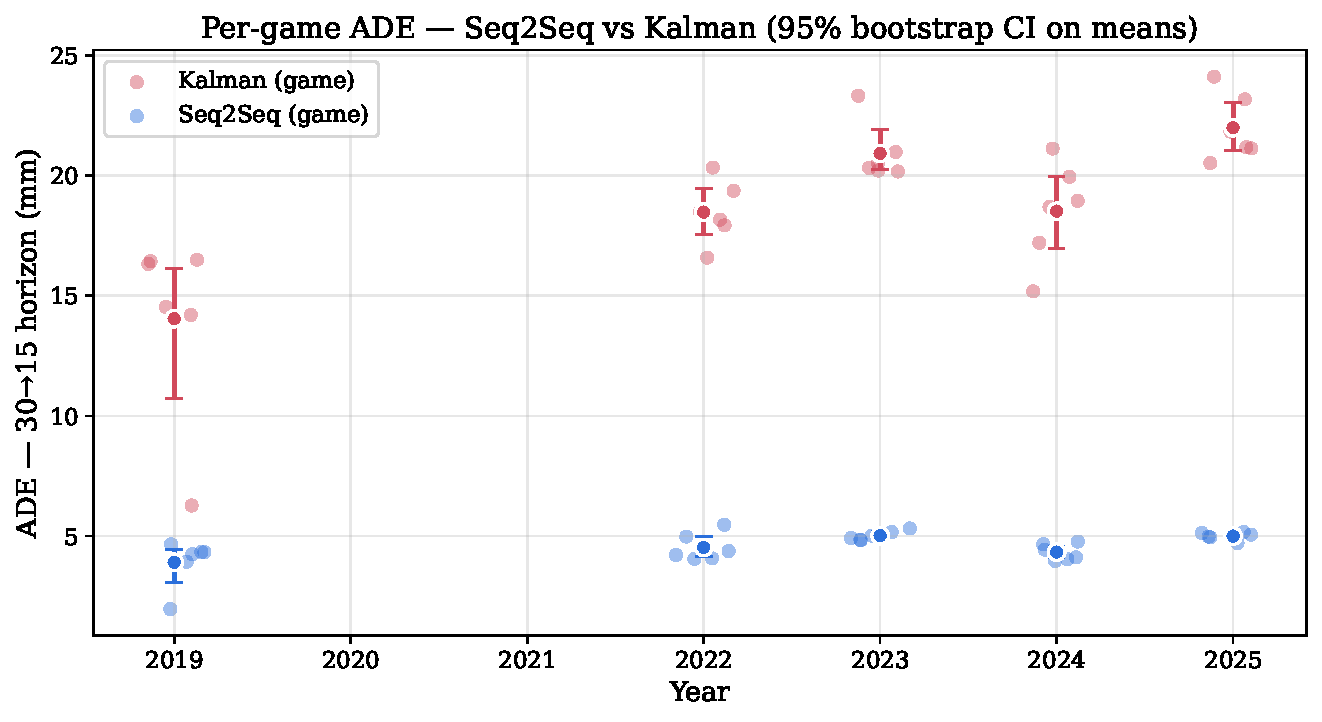
\includegraphics[width=0.86\linewidth]{4a_ade_year_per_game_pt}
\caption{ADE por jogo (Seq2Seq vs.\ Kalman, horizonte 30$\to$15) com IC
         95\,\% \emph{bootstrap} sobre as m\'edias anuais. Cada ponto
         \'e um jogo. A queda relativa sustentada em 2021--2025 \'e o
         sinal de drift que o restante do trabalho busca explicar.}
\label{fig:m1_ade_year}
\end{figure}

\subsubsection{Cauda do erro: raz\~ao p99/p50}

A Figura~\ref{fig:m1_p99} mostra que a raz\~ao $\mathrm{p99}/\mathrm{p50}$
do Seq2Seq cresce em 2021 (4{,}94 vs.\ 4{,}36 no baseline), confirmando
que o modelo n\~ao falha ``um pouco em tudo'' --- ele falha
desproporcionalmente em uma cauda crescente de trajet\'orias.

\begin{figure}[H]
\centering
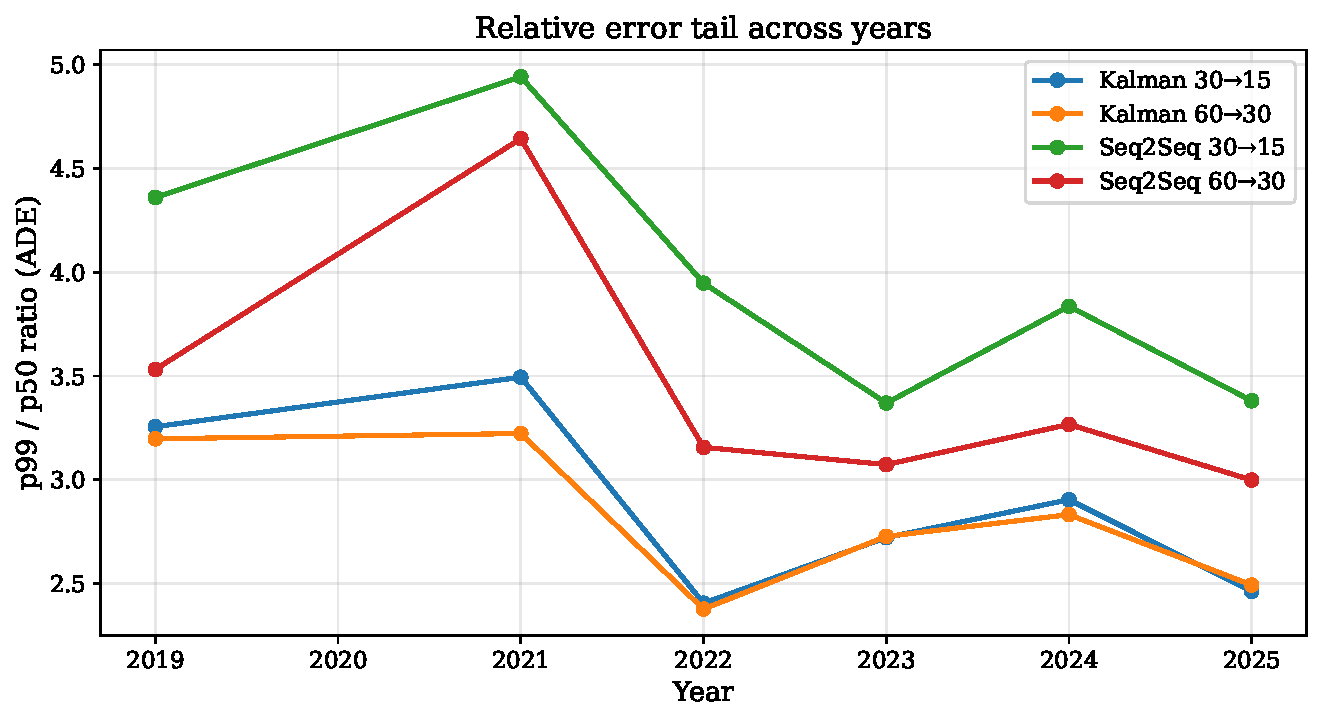
\includegraphics[width=0.78\linewidth]{3c_p99_p50_ratio_pt}
\caption{Raz\~ao $\mathrm{p99}/\mathrm{p50}$ do ADE por trajet\'oria,
         por (modelo, horizonte). Curvas crescentes para o Seq2Seq em
         ambos horizontes confirmam que o drift afeta primeiramente a
         cauda.}
\label{fig:m1_p99}
\end{figure}

\begin{table}[H]
\centering\small
\begin{tabular}{rlrrrr}
\toprule
\textbf{Ano} & \textbf{Modelo} & \textbf{p50 (mm)} & \textbf{p90 (mm)} & \textbf{p99 (mm)} & \textbf{p99/p50} \\
\midrule
2019 & Seq2Seq & 3{,}70  &  8{,}62 & 16{,}14 & 4{,}36 \\
2021 & Seq2Seq & 5{,}87  & 15{,}12 & 28{,}99 & 4{,}94 \\
2022 & Seq2Seq & 4{,}02  &  8{,}91 & 15{,}86 & 3{,}95 \\
2023 & Seq2Seq & 4{,}57  &  9{,}59 & 15{,}41 & 3{,}37 \\
2024 & Seq2Seq & 3{,}84  &  8{,}32 & 14{,}74 & 3{,}84 \\
\bottomrule
\end{tabular}
\caption{Percentis do ADE por trajet\'oria (Seq2Seq, horizonte
         30$\to$15). 2021 \'e o ano com cauda mais pesada
         absoluta; 2023 tem a menor raz\~ao $\mathrm{p99}/\mathrm{p50}$,
         indicando \emph{drift de m\'edia} mais que \emph{drift de cauda}.
         Fonte:
         \texttt{Relas/results/drift/01\_.../tail\_stats.csv}.}
\label{tab:tail}
\end{table}

\subsubsection{Histograma de ADE: 2019 vs.\ 2025}

\begin{figure}[H]
\centering
\begin{subfigure}[b]{0.49\textwidth}
\centering
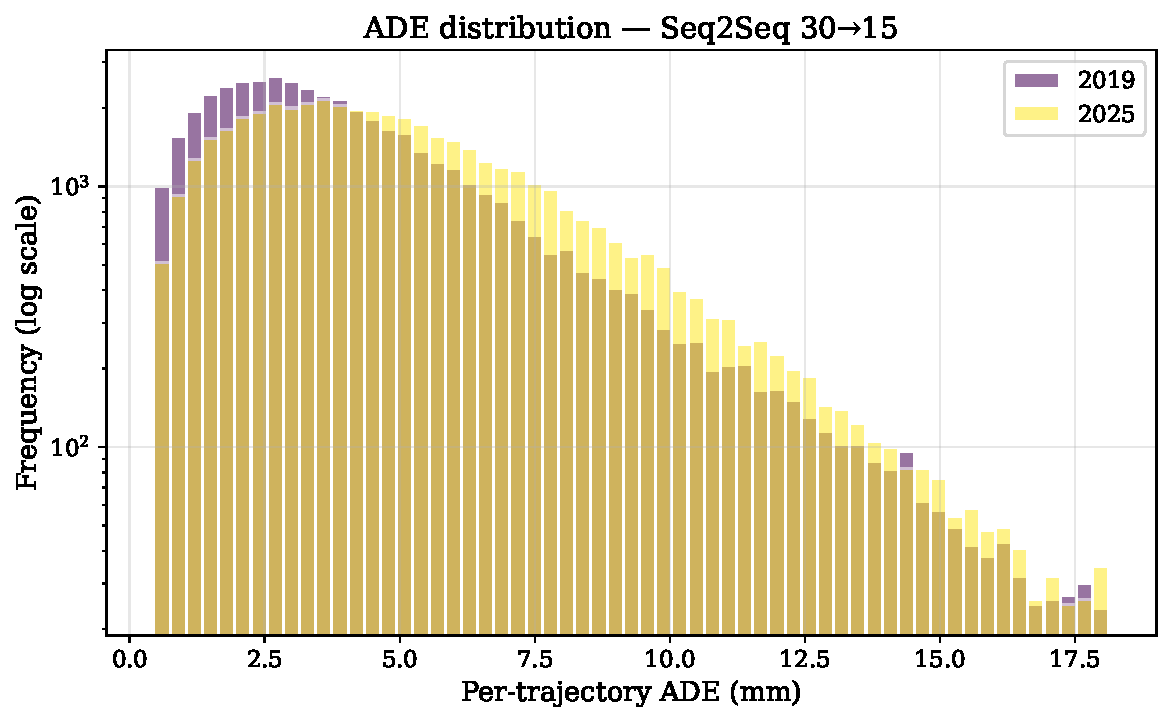
\includegraphics[width=\linewidth]{3a_ade_traj_hist_Seq2Seq_30_15_pt}
\caption{Seq2Seq, 30$\to$15.}
\end{subfigure}\hfill
\begin{subfigure}[b]{0.49\textwidth}
\centering
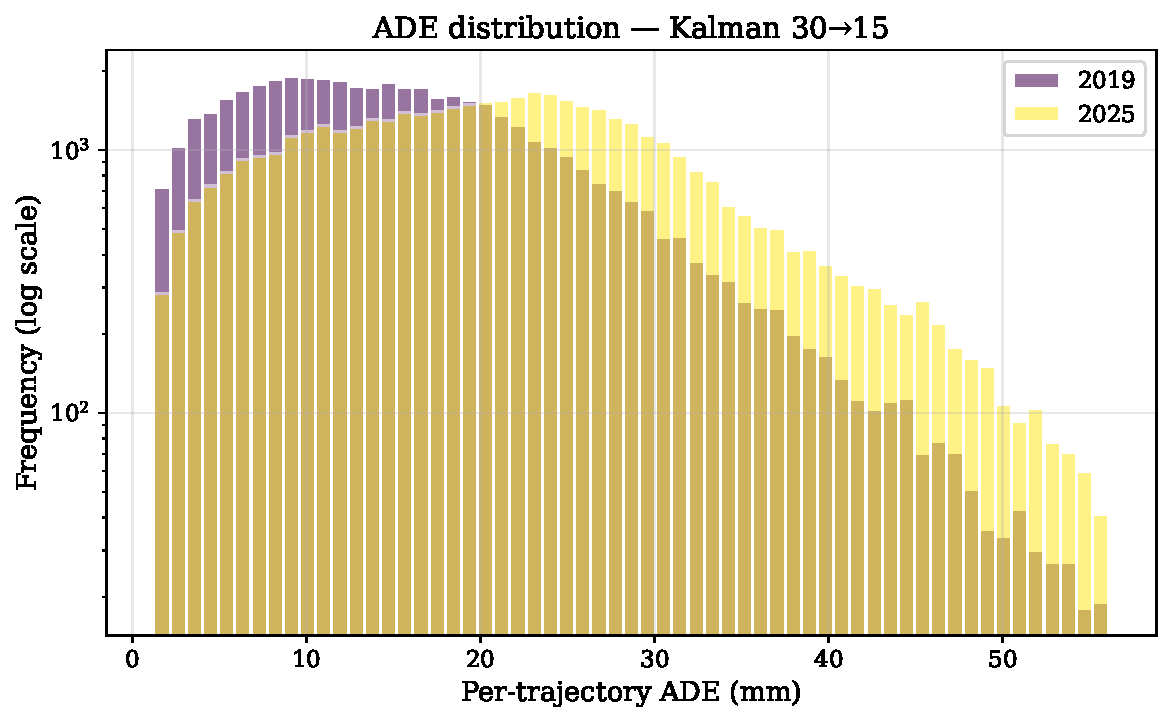
\includegraphics[width=\linewidth]{3a_ade_traj_hist_Kalman_30_15_pt}
\caption{Kalman, 30$\to$15.}
\end{subfigure}
\caption{Distribui\c{c}\~ao de ADE por trajet\'oria. Eixo $y$ em escala
         log. Em ambos os modelos a massa central \'e pr\'oxima entre
         2019 e 2025, mas a cauda direita engorda visivelmente em
         2025. Esse contraste motiva a decomposi\c{c}\~ao IW da
         Se\c{c}\~ao~\ref{sec:iw}.}
\label{fig:m1_hist}
\end{figure}

\subsubsection{Drift por janela (intra-jogo)}

\begin{figure}[H]
\centering
\begin{subfigure}[b]{0.49\textwidth}
\centering
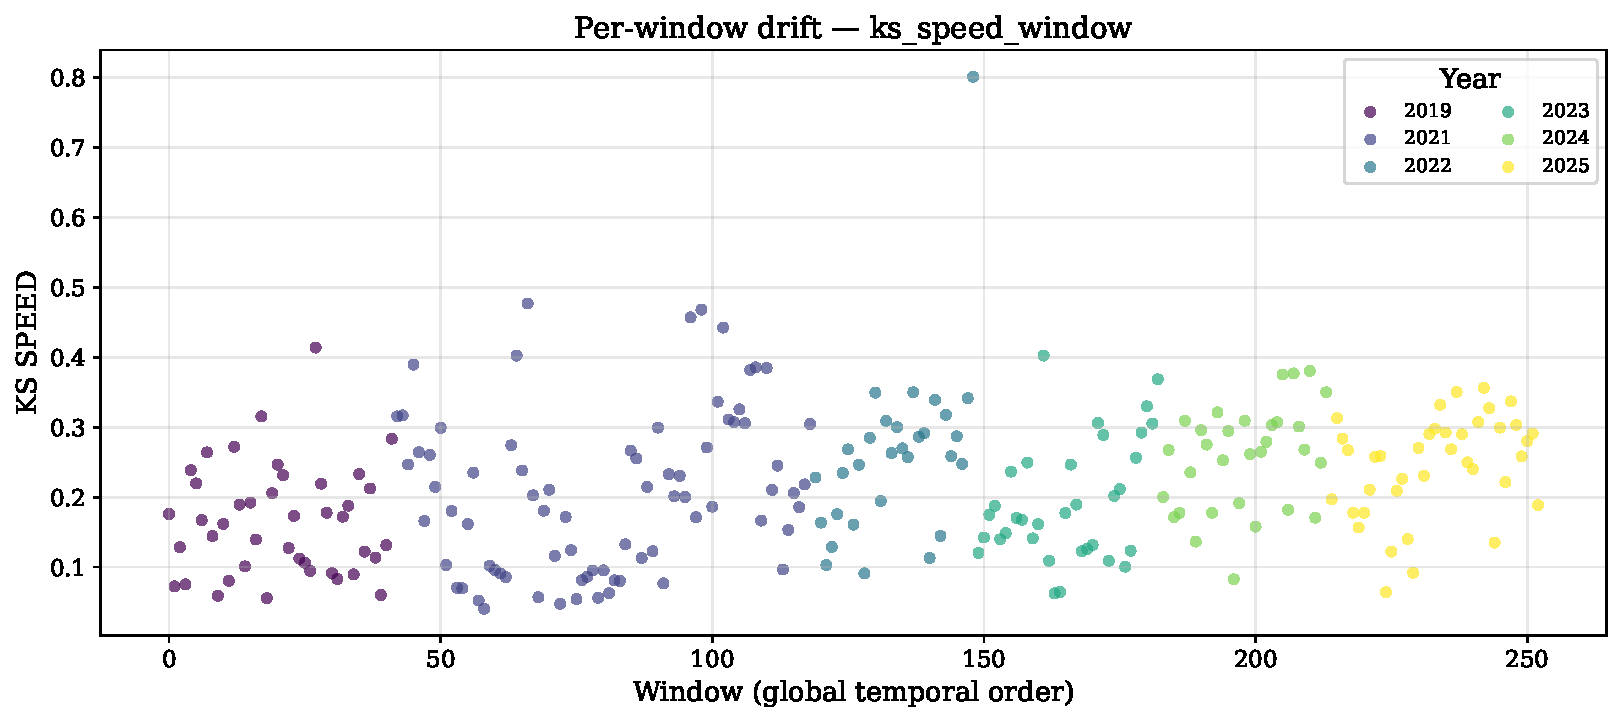
\includegraphics[width=\linewidth]{2a_window_timeline_ks_speed_window_pt}
\caption{KS de velocidade --- timeline.}
\end{subfigure}\hfill
\begin{subfigure}[b]{0.49\textwidth}
\centering
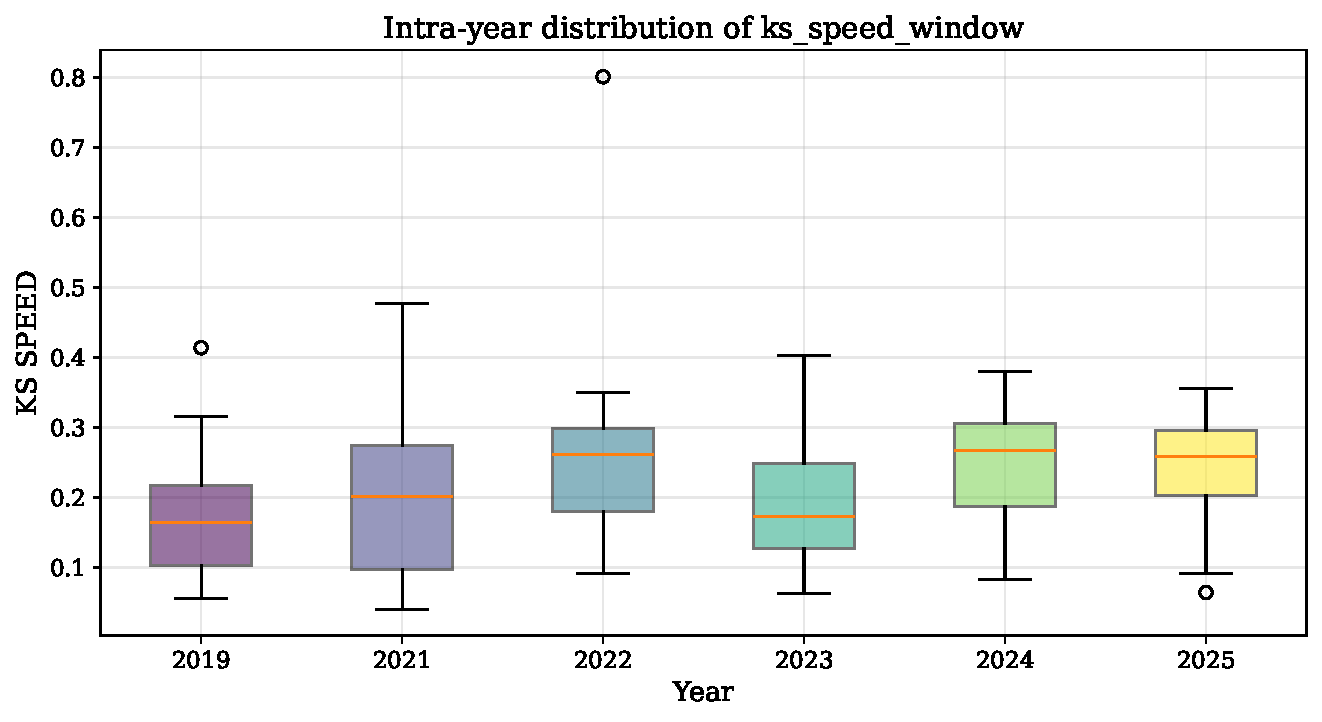
\includegraphics[width=\linewidth]{2b_window_box_ks_speed_window_pt}
\caption{KS de velocidade --- boxplot por ano.}
\label{fig:m1_window_box}
\end{subfigure}

\vspace{0.3em}

\begin{subfigure}[b]{0.49\textwidth}
\centering
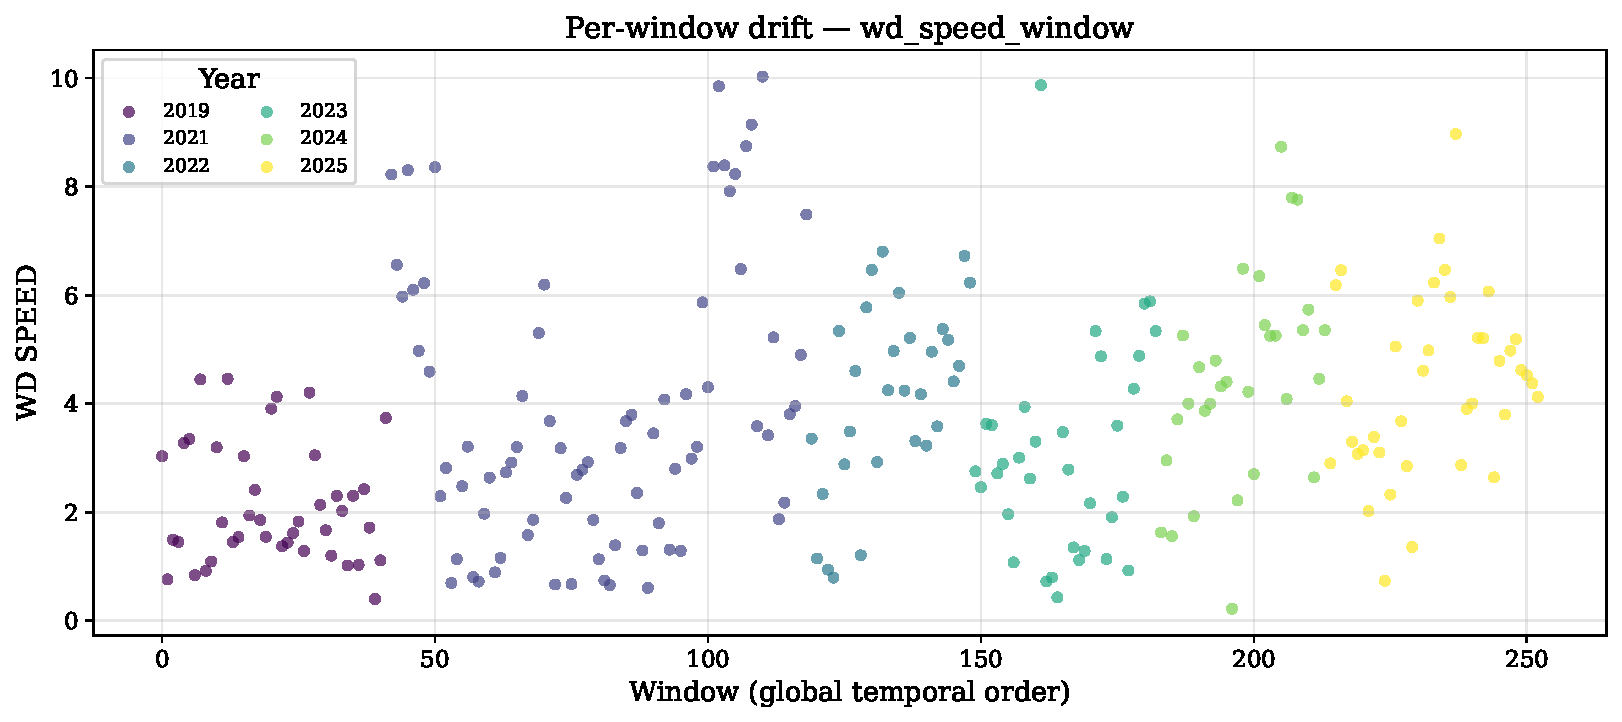
\includegraphics[width=\linewidth]{2a_window_timeline_wd_speed_window_pt}
\caption{Wasserstein de velocidade --- timeline.}
\end{subfigure}\hfill
\begin{subfigure}[b]{0.49\textwidth}
\centering
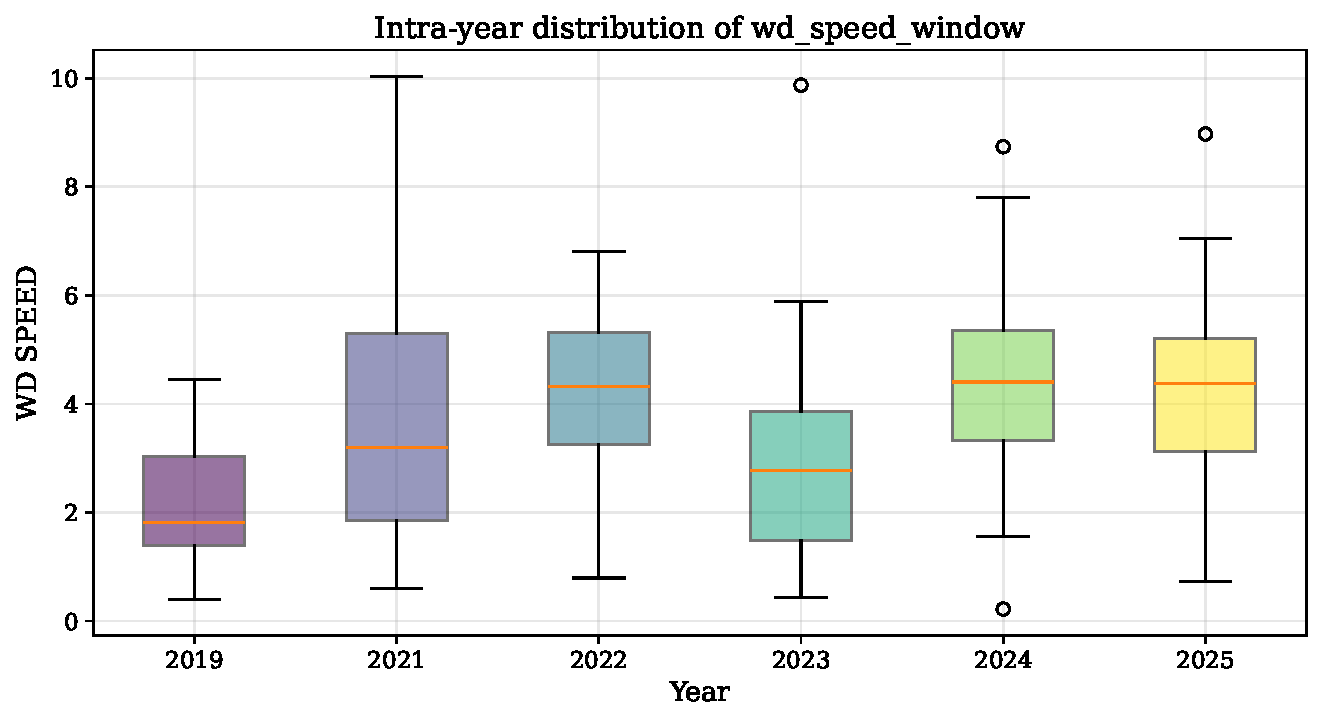
\includegraphics[width=\linewidth]{2b_window_box_wd_speed_window_pt}
\caption{Wasserstein de velocidade --- boxplot por ano.}
\end{subfigure}
\caption{Drift de \emph{velocidade} por janela contra o baseline 2019,
         medido por duas estat\'isticas independentes: KS (acima) e
         Wasserstein (abaixo). As duas concordam qualitativamente:
         medianas crescentes em 2021 e 2023+, com cauda longa em 2021.
         Fonte: \texttt{per\_window\_drift.csv}.}
\label{fig:m1_window}
\end{figure}

\begin{figure}[H]
\centering
\begin{subfigure}[b]{0.49\textwidth}
\centering
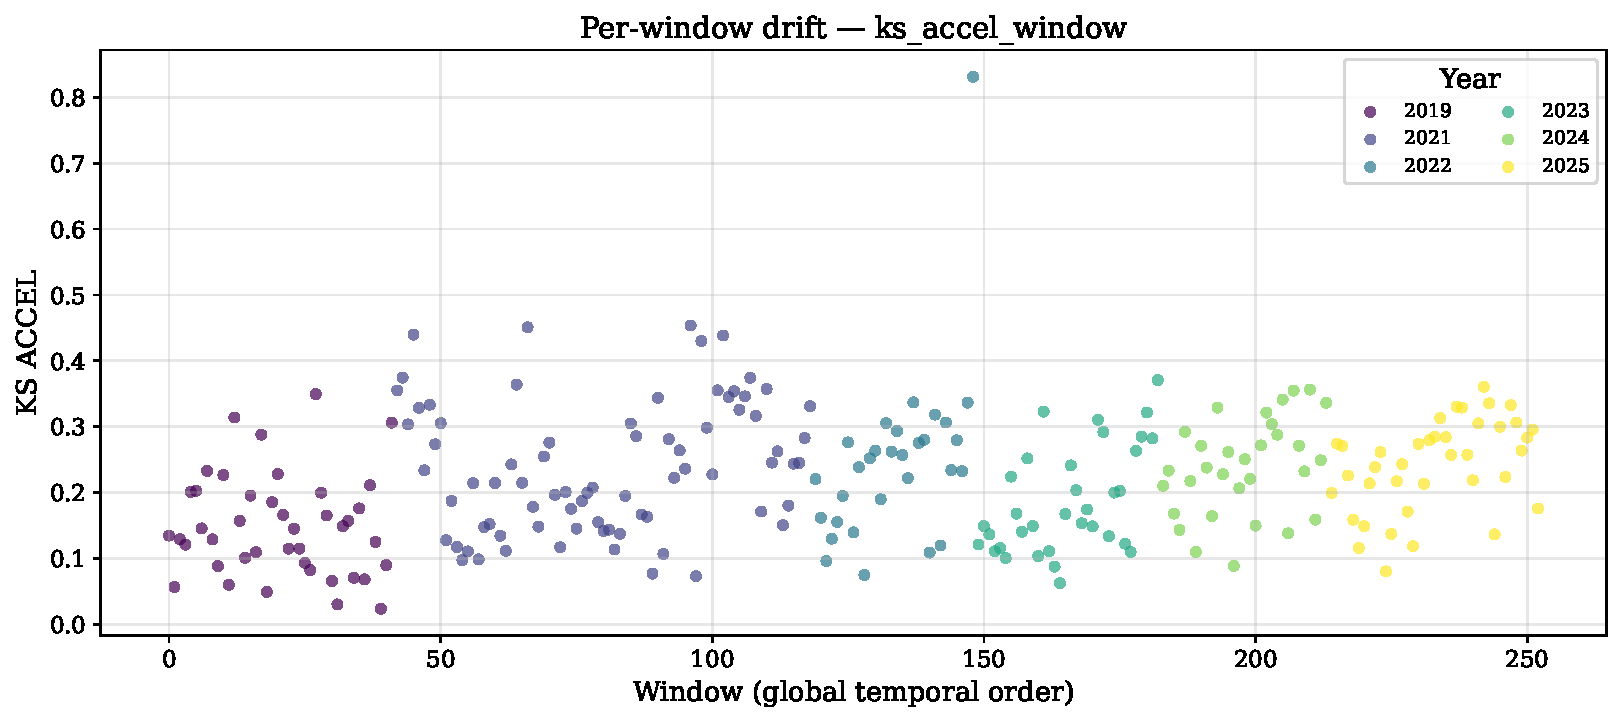
\includegraphics[width=\linewidth]{2a_window_timeline_ks_accel_window_pt}
\caption{KS de acelera\c{c}\~ao --- timeline.}
\end{subfigure}\hfill
\begin{subfigure}[b]{0.49\textwidth}
\centering
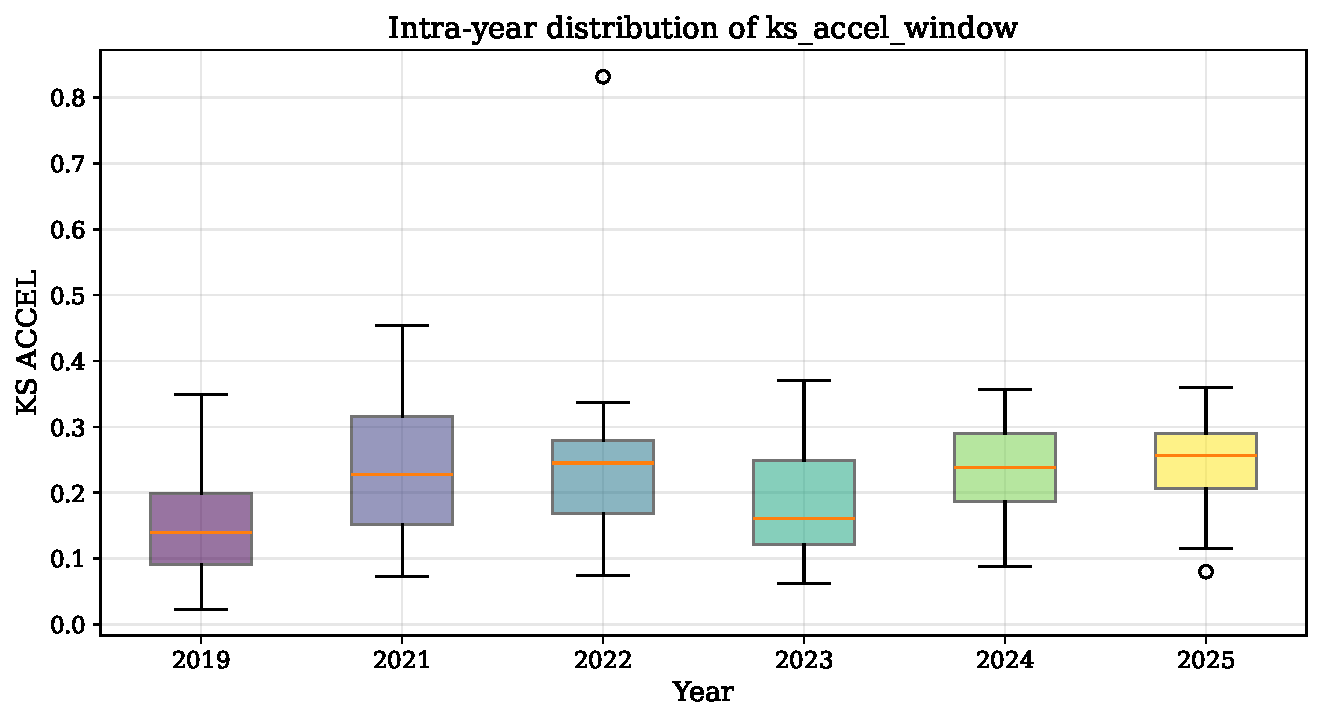
\includegraphics[width=\linewidth]{2b_window_box_ks_accel_window_pt}
\caption{KS de acelera\c{c}\~ao --- boxplot por ano.}
\end{subfigure}

\vspace{0.3em}

\begin{subfigure}[b]{0.49\textwidth}
\centering
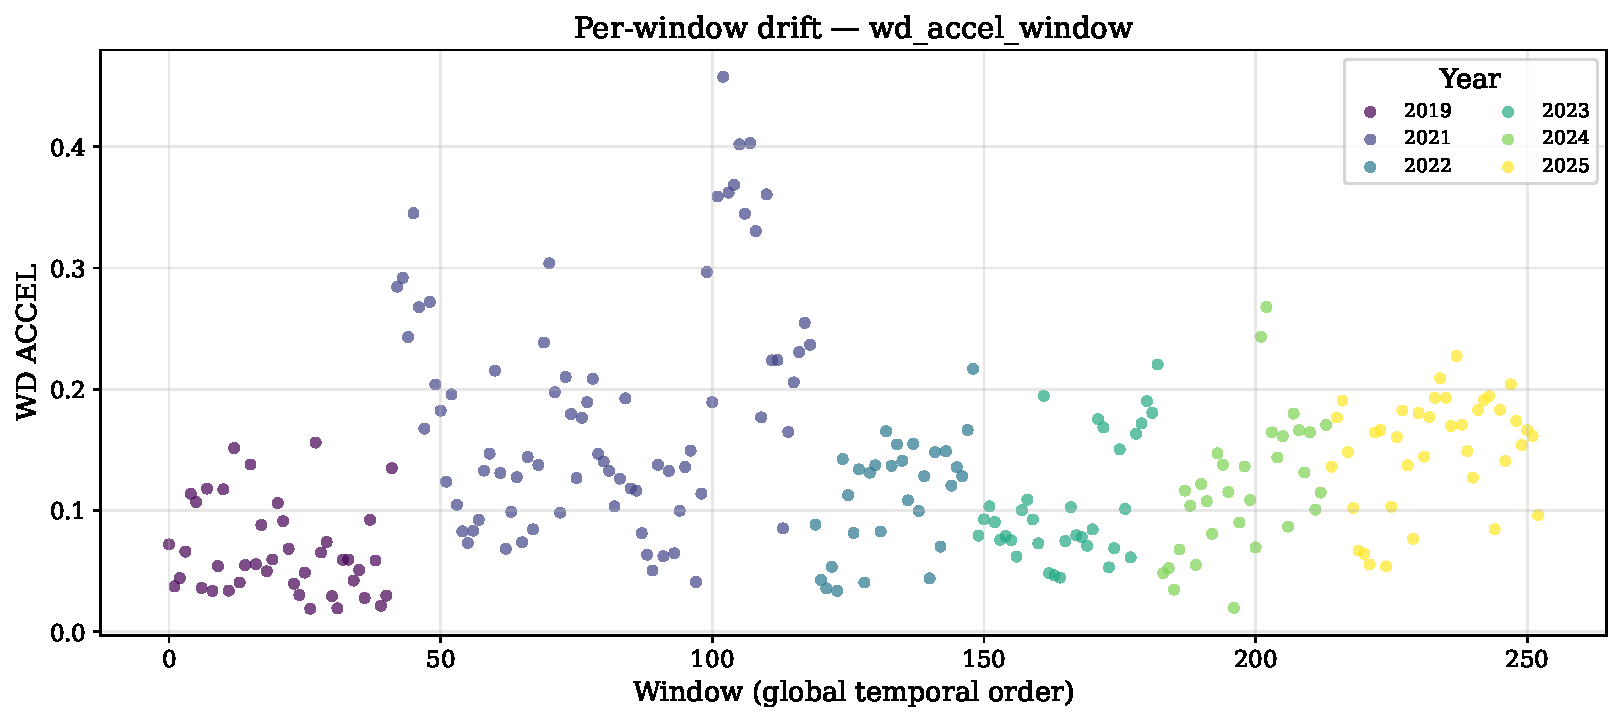
\includegraphics[width=\linewidth]{2a_window_timeline_wd_accel_window_pt}
\caption{Wasserstein de acelera\c{c}\~ao --- timeline.}
\end{subfigure}\hfill
\begin{subfigure}[b]{0.49\textwidth}
\centering
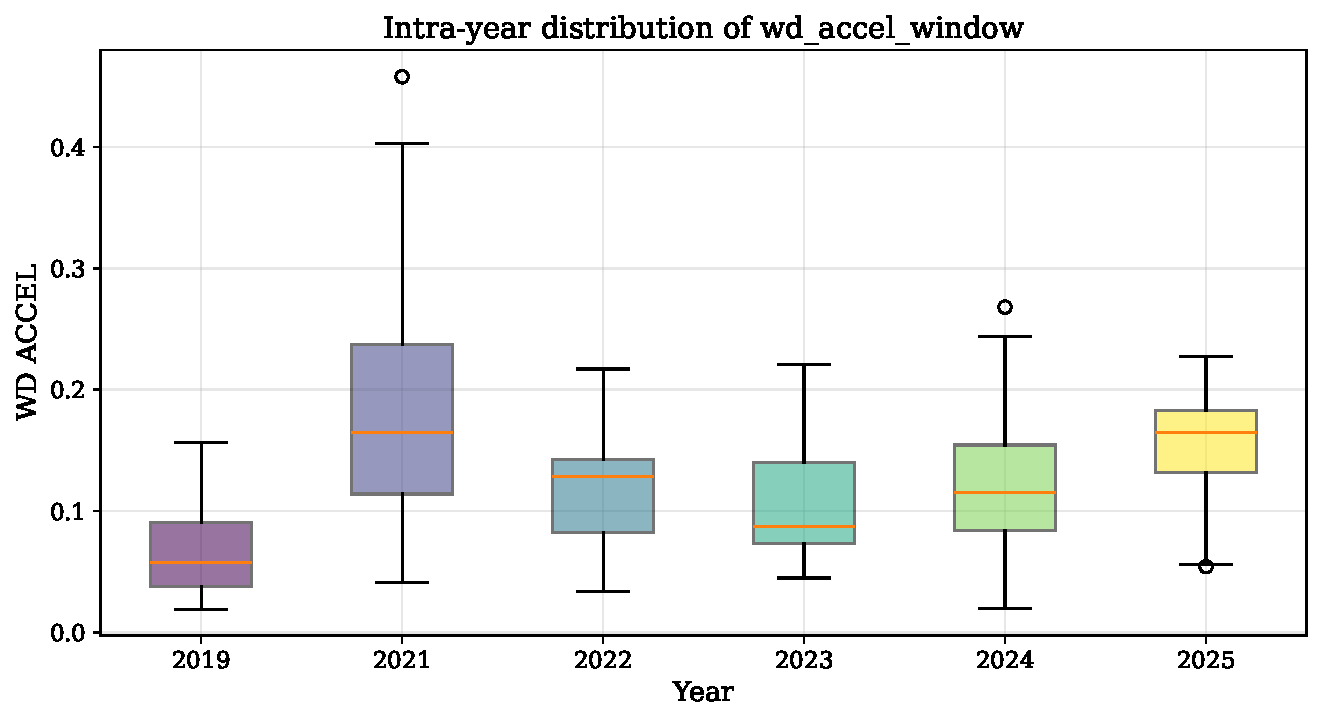
\includegraphics[width=\linewidth]{2b_window_box_wd_accel_window_pt}
\caption{Wasserstein de acelera\c{c}\~ao --- boxplot por ano.}
\end{subfigure}
\caption{Drift de \emph{acelera\c{c}\~ao} por janela contra o baseline
         2019, medido por KS (acima) e Wasserstein (abaixo). O padr\~ao
         quantitativo \'e parecido com o da velocidade, mas com
         magnitudes maiores em 2021.}
\label{fig:m1_window_accel}
\end{figure}

\subsubsection{ADE vs.\ features cinem\'aticas}

\begin{figure}[H]
\centering
\begin{subfigure}[b]{0.32\textwidth}
\centering
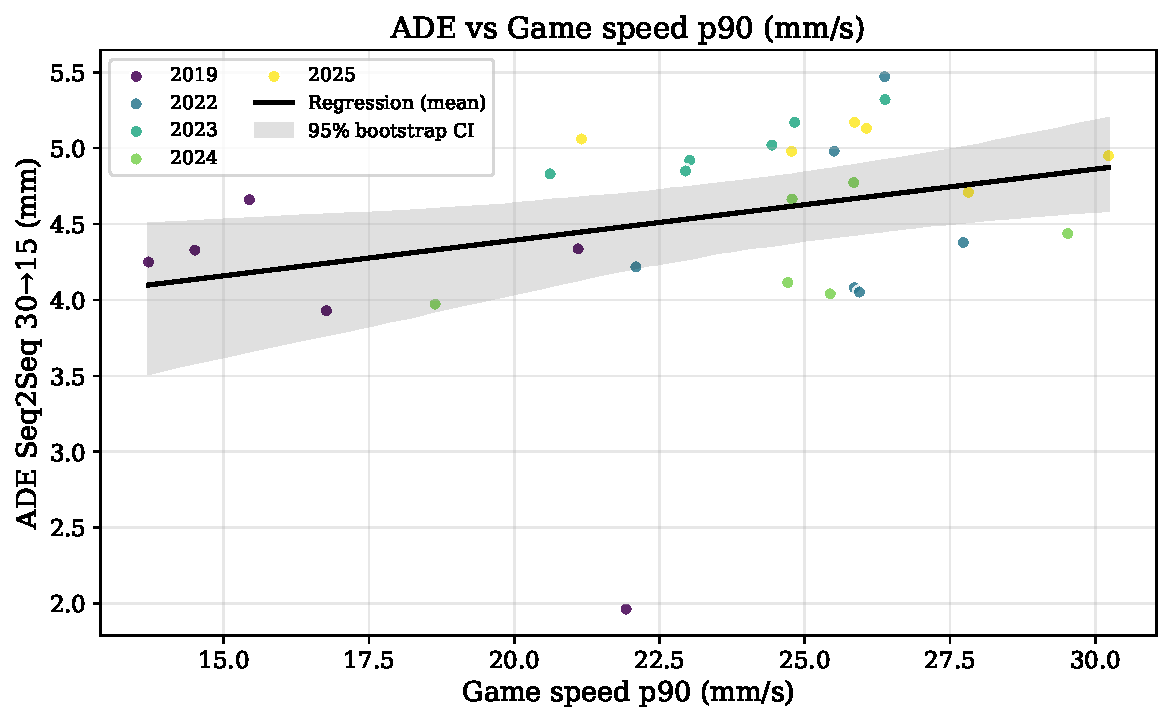
\includegraphics[width=\linewidth]{4b_ade_vs_speed_p90_pt}
\caption{vs.\ \texttt{speed\_p90}.}
\end{subfigure}\hfill
\begin{subfigure}[b]{0.32\textwidth}
\centering
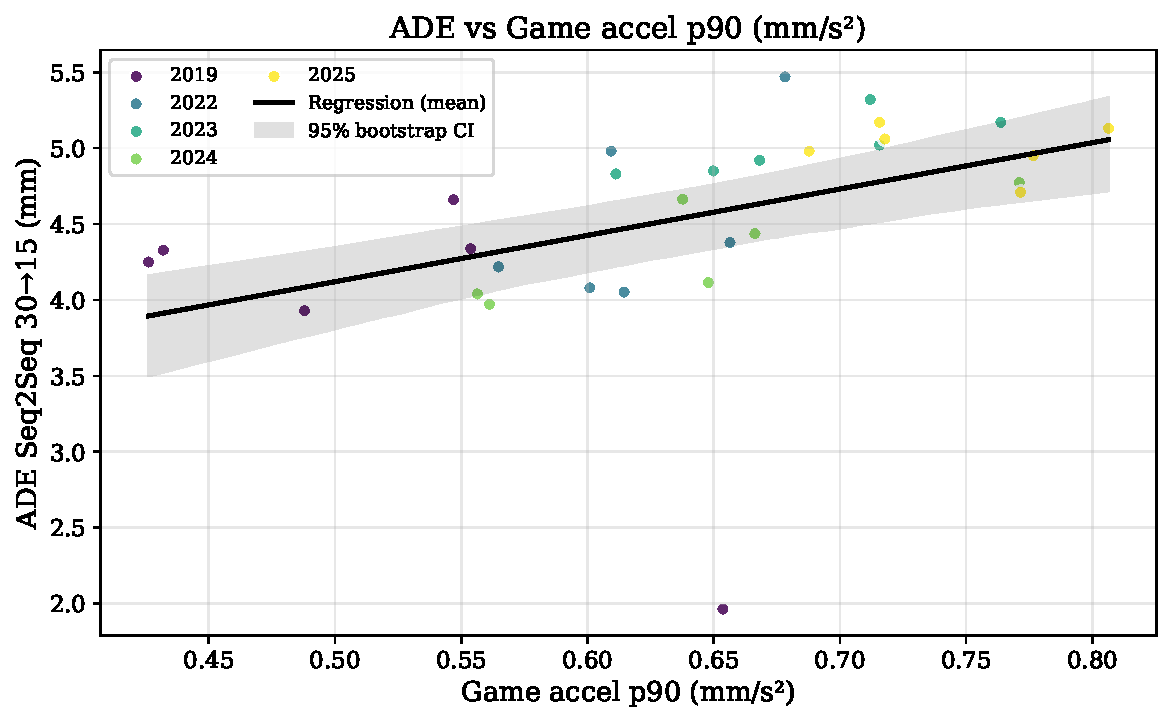
\includegraphics[width=\linewidth]{4b_ade_vs_accel_p90_pt}
\caption{vs.\ \texttt{accel\_p90}.}
\end{subfigure}\hfill
\begin{subfigure}[b]{0.32\textwidth}
\centering
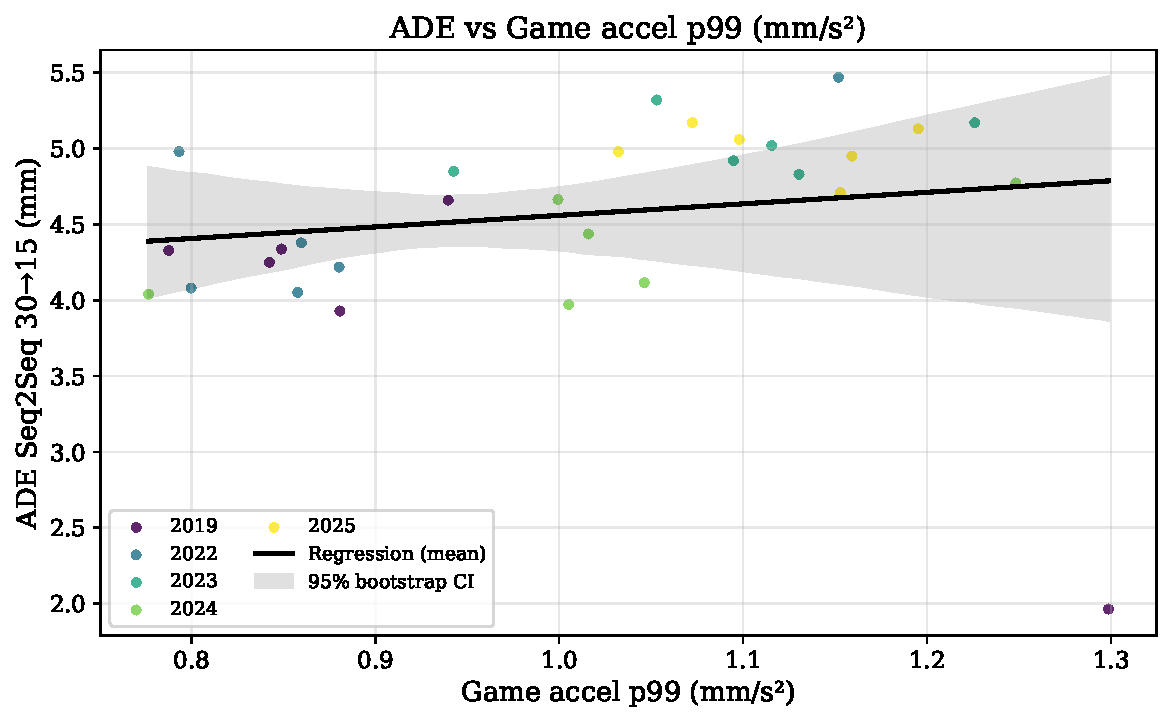
\includegraphics[width=\linewidth]{4b_ade_vs_accel_p99_pt}
\caption{vs.\ \texttt{accel\_p99}.}
\end{subfigure}
\caption{ADE do Seq2Seq (30$\to$15) por jogo contra percentis de
         velocidade e acelera\c{c}\~ao. Cada ponto \'e um jogo,
         colorido pelo ano. Reta de regress\~ao linear com IC\,95\,\%
         \emph{bootstrap}. O \texttt{accel\_p99} \'e a feature de maior
         correla\c{c}\~ao individual com o ADE.}
\label{fig:m1_ade_vs}
\end{figure}

\begin{figure}[H]
\centering
\begin{subfigure}[b]{0.49\textwidth}
\centering
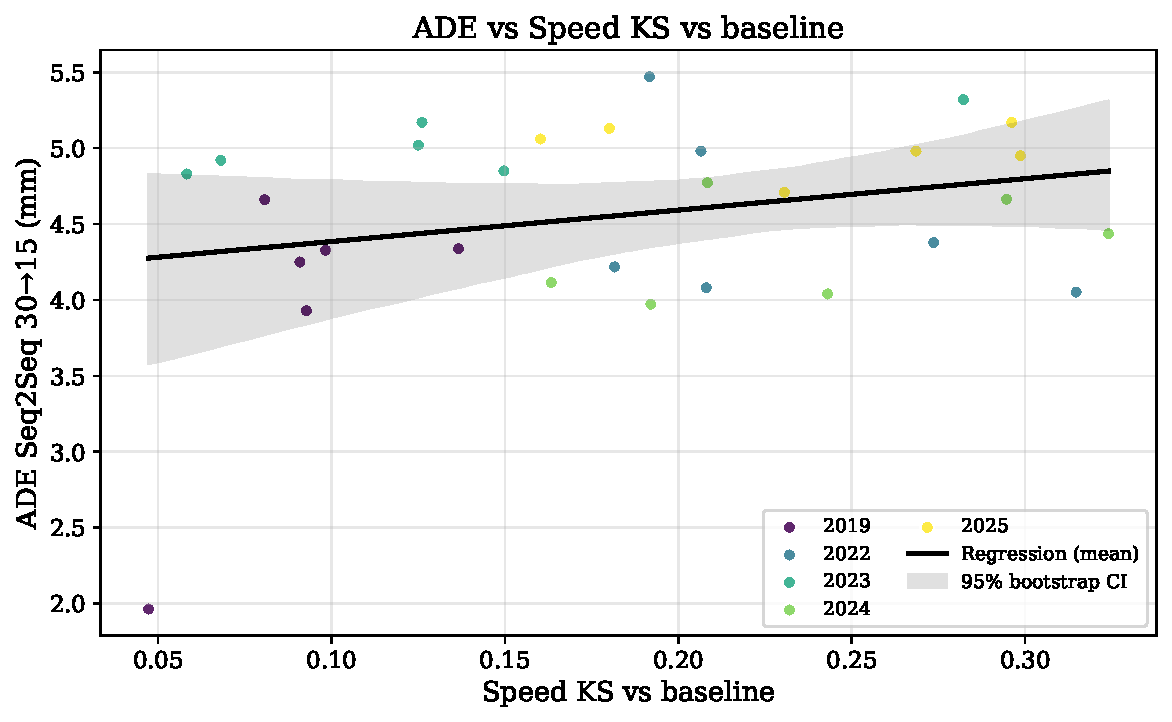
\includegraphics[width=\linewidth]{4b_ade_vs_ks_speed_pt}
\caption{vs.\ \texttt{ks\_speed}.}
\end{subfigure}\hfill
\begin{subfigure}[b]{0.49\textwidth}
\centering
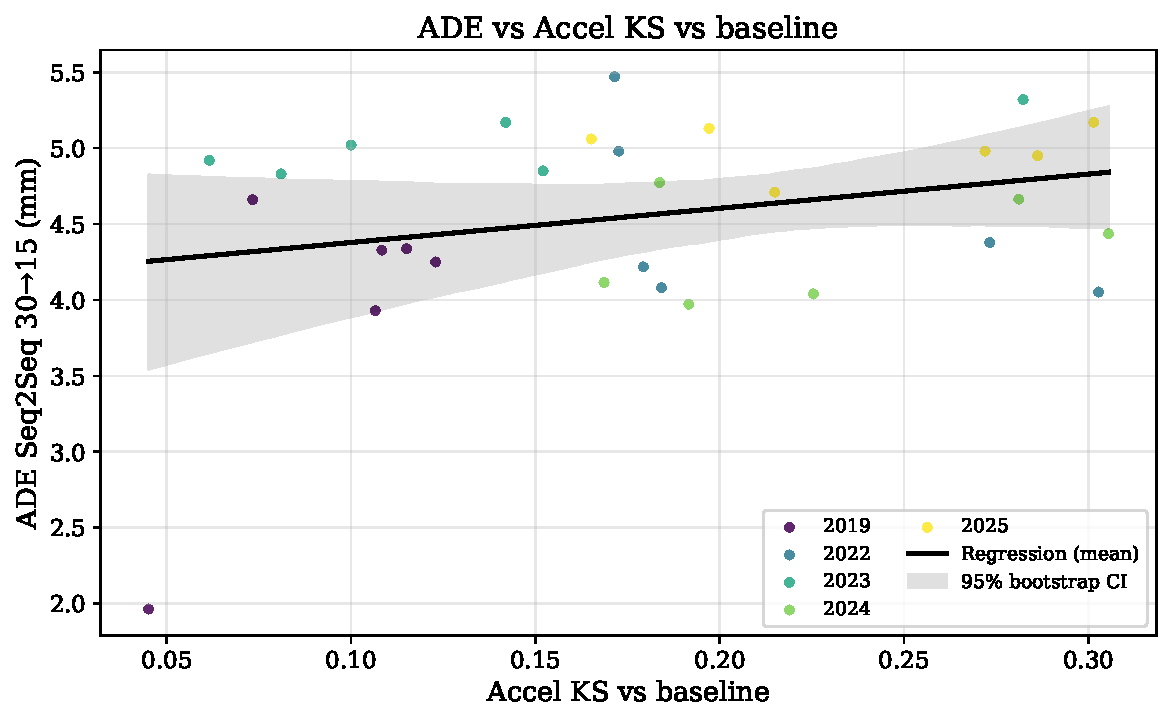
\includegraphics[width=\linewidth]{4b_ade_vs_ks_accel_pt}
\caption{vs.\ \texttt{ks\_accel}.}
\end{subfigure}

\vspace{0.3em}

\begin{subfigure}[b]{0.49\textwidth}
\centering
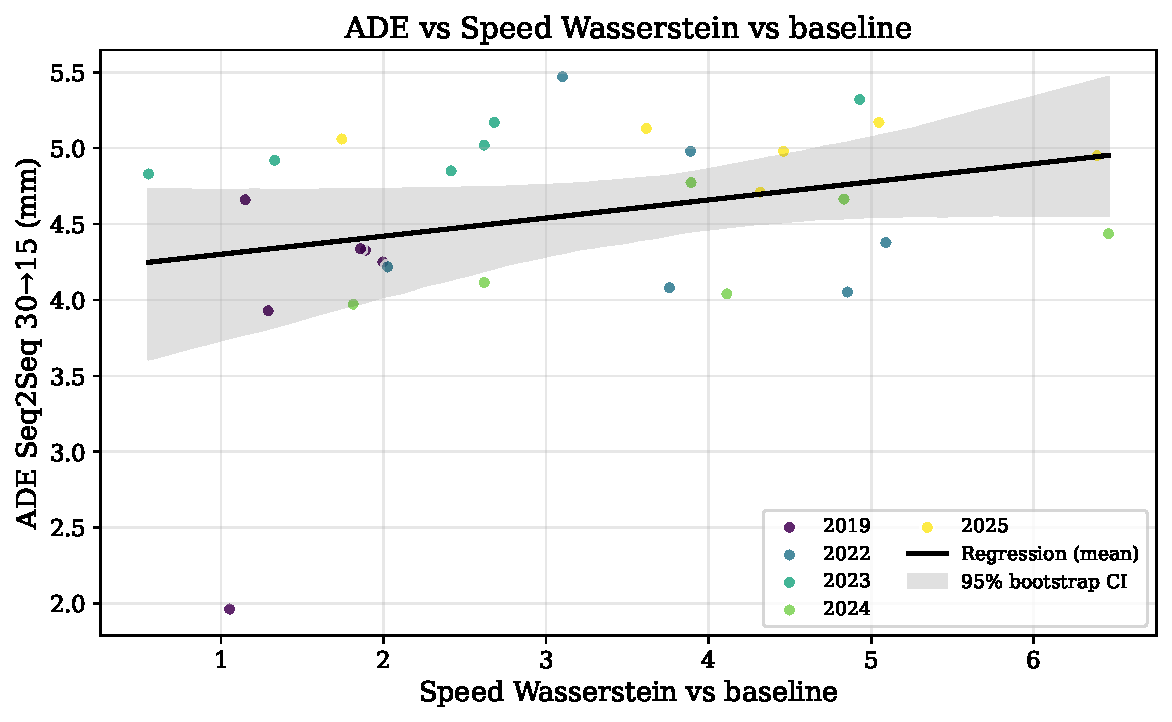
\includegraphics[width=\linewidth]{4b_ade_vs_wd_speed_pt}
\caption{vs.\ \texttt{wd\_speed}.}
\end{subfigure}\hfill
\begin{subfigure}[b]{0.49\textwidth}
\centering
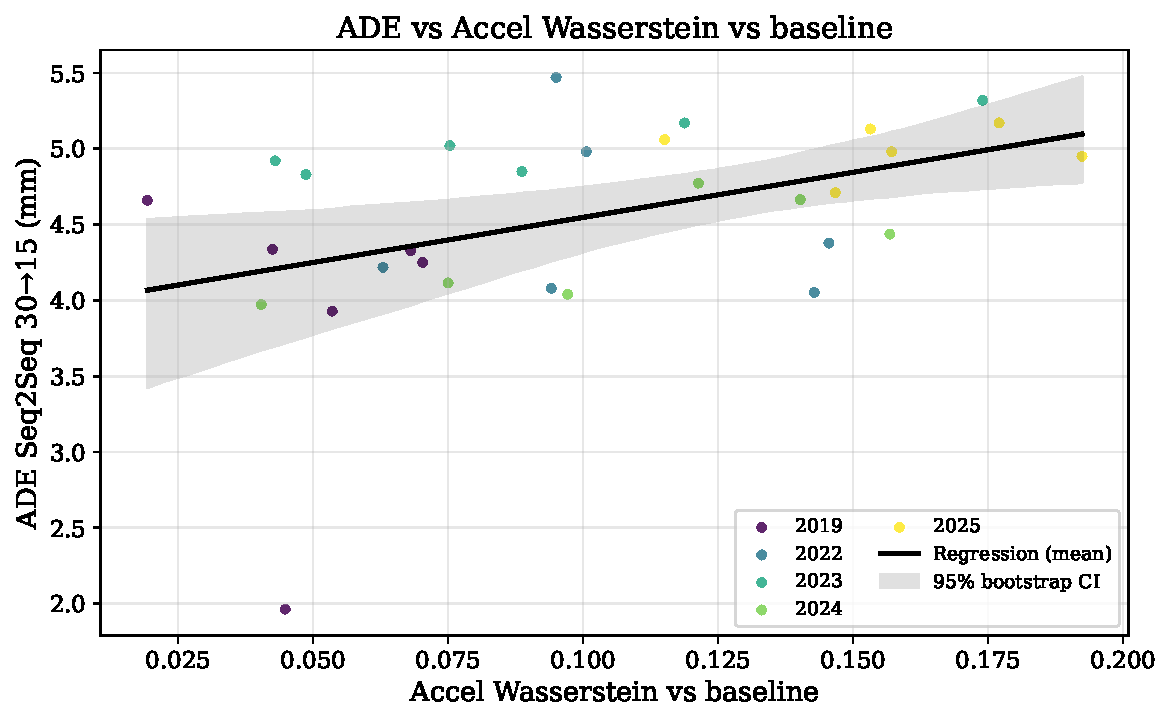
\includegraphics[width=\linewidth]{4b_ade_vs_wd_accel_pt}
\caption{vs.\ \texttt{wd\_accel}.}
\end{subfigure}
\caption{ADE do Seq2Seq (30$\to$15) por jogo contra as quatro
         estat\'isticas de drift de janela (KS e Wasserstein para
         velocidade e acelera\c{c}\~ao). KS e Wasserstein concordam
         qualitativamente; a acelera\c{c}\~ao apresenta sinal mais
         forte que a velocidade.}
\label{fig:m1_ade_vs_drift}
\end{figure}

\subsubsection{Mapa de correla\c{c}\~oes}

\begin{figure}[H]
\centering
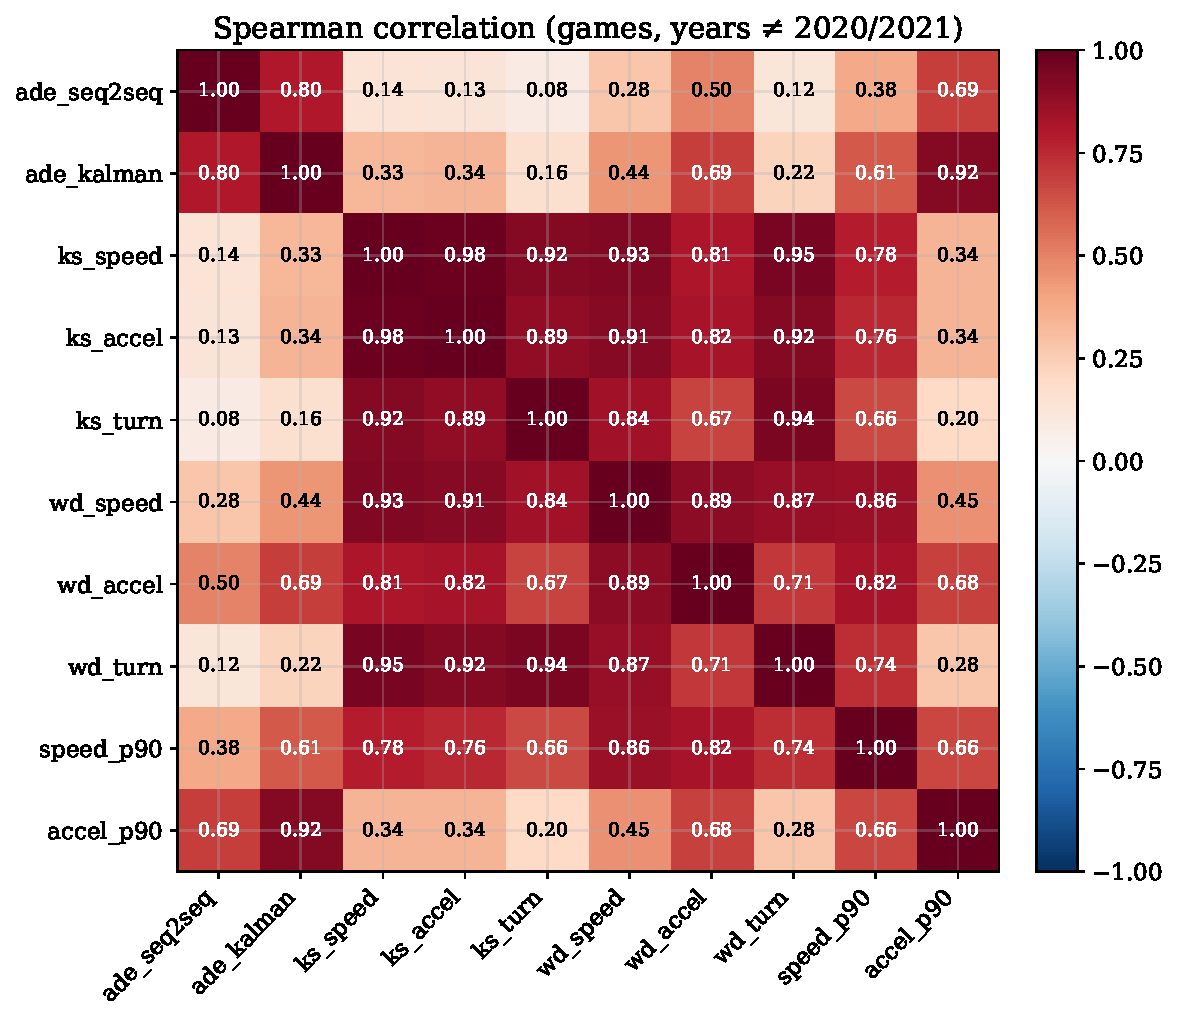
\includegraphics[width=0.72\linewidth]{4d_corr_spearman_pt}
\caption{Correla\c{c}\~ao de Spearman entre ADE por jogo e features de
         drift, restrito a anos $\neq$ 2020/2021. As correla\c{c}\~oes
         mais fortes ficam entre o ADE do Seq2Seq e features de
         acelera\c{c}\~ao de cauda (\texttt{accel\_p90, accel\_p99}),
         antecipando o resultado per-feature do M\^es~3.}
\label{fig:m1_corr}
\end{figure}

% ============================================================================
\section{Notebook 02 --- Detec\c{c}\~ao no stream (M\^es 2)}
% ============================================================================

O notebook \texttt{02\_deteccao\_no\_stream} substitui infer\^encia
visual por testes estat\'isticos de \emph{change-point detection}.
Tr\^es detectores online (ADWIN, Page-Hinkley, KSWIN) e um offline
(Pelt) s\~ao aplicados sobre os streams definidos no notebook 01,
e dois experimentos auxiliares quantificam null e lat\^encia.
A leitura do M\^es 9 (Se\c{c}\~ao~\ref{sec:mes9}) re-otimiza
essa parametriza\c{c}\~ao e produz o detetor operacional final.

\subsection{Concept drift online (ADWIN + Page-Hinkley)}
\label{sec:m2_adwin_ph}

\paragraph{ADWIN --- como funciona.}
\textbf{ADWIN} (\emph{Adaptive Windowing}~--- Janelamento Adaptativo) \cite{adwin} \'e um detector online que mant\'em uma janela $W$ de observa\c{c}\~oes recentes e verifica continuamente se ela pode ser particionada em duas sub-janelas com m\'edias significativamente diferentes.

\emph{Analogia intuitiva:} imagine um inspetor de qualidade que mant\'em um hist\'orico das \'ultimas medidas de erro de uma m\'aquina e, em cada nova medi\c{c}\~ao, testa todas as poss\'iveis divis\~oes desse hist\'orico em um ``per\'iodo antigo'' e um ``per\'iodo recente''. Se a m\'edia do per\'iodo recente for significativamente diferente da m\'edia do per\'iodo antigo, o inspetor conclui que algo mudou~--- dispara um alarme e descarta os dados antigos, resetando a janela.

\emph{Mecanismo formal:} ADWIN particiona iterativamente a janela $W$ em todas as poss\'iveis divis\~oes $(W_0, W_1)$, sendo $W_0$ o trecho mais antigo e $W_1$ o mais recente. Para cada par, calcula $|\hat\mu_{W_0} - \hat\mu_{W_1}|$ (diferen\c{c}a de m\'edias) e compara com um limiar $\epsilon_\mathrm{cut}(\delta)$ derivado da \textbf{desigualdade de Hoeffding}~--- um resultado matem\'atico que garante uma prob\-a\-bi\-li\-da\-de de falso alarme de no m\'aximo $\delta$ (o par\^ametro de confian\c{c}a). Quando $|\hat\mu_{W_0} - \hat\mu_{W_1}| > \epsilon_\mathrm{cut}$, o ADWIN descarta $W_0$ (considera que o regime mudou) e dispara um alarme.

\emph{Par\^ametros relevantes neste trabalho:}
\begin{itemize}[leftmargin=1.4em,itemsep=1pt]
    \item $\delta$ (\texttt{delta}): n\'ivel de confian\c{c}a~--- controla a sensibilidade. Quanto menor $\delta$, mais conservador o detector (menos falsos alarmes, mas tamb\'em menor sensibilidade a drift real). O valor \'otimo encontrado foi $\delta = 10^{-7}$.
    \item \texttt{min\_window}: tamanho m\'inimo da janela antes que o detector possa disparar~--- evita alarmes prec\'oces no in\'icio do stream.
    \item \texttt{cooldown}: n\'umero de trajet\'orias ap\'os um alarme durante as quais o detector n\~ao dispara novamente~--- evita alarmes em r\'apida sucess\~ao.
    \item \texttt{max\_window}: tamanho m\'aximo da janela~--- evita que o detector acumule mem\'oria excessiva.
\end{itemize}

\emph{Comportamento t\'ipico em streams i.i.d.\ Gaussianos} (dados independentes sem drift real): ADWIN \'e \emph{matematicamente conservador}~--- mesmo com $\delta\!=\!0{,}99$ (muito permissivo), a literatura \cite{lu2019,gama2014} reporta ARL\,$\gtrsim\!10^3$ amostras antes de um falso alarme.

\paragraph{Page-Hinkley --- como funciona.}
O teste de \citet{page_hinkley}, originalmente desenvolvido para controle estat\'istico de qualidade industrial (detectar quando uma linha de produ\c{c}\~ao sai das especifica\c{c}\~oes), detecta aumentos sustentados na m\'edia de uma s\'erie temporal acumulando desvios:
\[
g_t = \max\left(0,\, g_{t-1} + (x_t - \bar{x}_t - \delta)\right),\quad
\mathrm{alarme\ se\ } g_t - \min_{s\leq t} g_s > \lambda
\]
onde $\delta$ \'e o \emph{slack} (toler\^ancia a ru\'ido~--- pequenas flutua\c{c}\~oes abaixo de $\delta$ n\~ao contribuem para a acumula\c{c}\~ao) e $\lambda$ \'e o threshold de alarme.

\emph{Analogia intuitiva:} imagine marcar na parede a diferen\c{c}a acumulada entre o erro atual e a m\'edia hist\'orica. Se a marca na parede atingir uma altura cr\'itica $\lambda$ acima da posi\c{c}\~ao mais baixa j\'a registrada, o detector conclui que a m\'edia aumentou~--- dispara alarme. A vantagem sobre o ADWIN \'e a extrema simplicidade computacional; a desvantagem \'e a necessidade de especificar $\lambda$ e $\delta$ em rela\c{c}\~ao \`a escala dos dados.

Neste trabalho, o Page-Hinkley \'e tamb\'em aplicado de forma \textbf{agregada} (Frente B do M\^es 9): em vez de processar cada trajet\'oria individualmente, calcula-se a m\'edia \emph{trimmed-mean} (m\'edia ap\'os remover os 5\% maiores e menores valores~--- mais robusta a outliers) de janelas de $N$ trajet\'orias consecutivas, e o PH opera sobre essa s\'erie agregada.

ADWIN e Page-Hinkley s\~ao aplicados sobre o stream de \texttt{ade\_traj}
ordenado por (year, match\_id, traj\_id), tanto para o Seq2Seq como para
o Kalman determin\'istico em paralelo. O contraste \'e informativo:
drift no Kalman = drift no comportamento do alvo; drift apenas no
Seq2Seq = miscalibra\c{c}\~ao do modelo treinado.

\paragraph{Itera\c{c}\~oes de calibra\c{c}\~ao (v1, v2, v3).}
A parametriza\c{c}\~ao passou por tr\^es vers\~oes; a literatura
\cite{gama2014,lu2019,mouss2004} \'e clara: o crit\'erio relevante \'e
o ARL sob null, n\~ao um threshold absoluto.

\begin{enumerate}[leftmargin=1.4em,itemsep=2pt]
    \item \textbf{v1 (defaults da literatura).} \texttt{delta\,=\,0{,}002}
          (ADWIN), \texttt{threshold\,=\,5\,mm} (PH) ---
          $\sim$\,40\,217 alarmes em 290\,k trajet\'orias, satura\c{c}\~ao trivial.
    \item \textbf{v2 (defaults absolutos, M\^es~5).}
          \texttt{delta\,=\,1\sci{-4}} (ADWIN),
          \texttt{threshold\,=\,100\,mm} e \texttt{delta\,=\,2\,mm}
          (PH). Reduziu para $\sim$\,478 alarmes ADWIN e $\sim$\,721
          alarmes PH no Seq2Seq, mas \emph{n\~ao escala} entre modelos.
    \item \textbf{v3 (baseline-relative \emph{adaptativa}, M\^es~6).}
          Par\^ametros como m\'ultiplos do MAD do baseline 2019 do
          \emph{pr\'oprio} modelo, e ambos os detectores ganham
          \emph{cooldown} p\'os-alarme.
\end{enumerate}

A varredura de calibra\c{c}\~ao
(\texttt{sweep\_concept\_drift\_calibration.py}, sa\'ida em
\texttt{concept\_drift\_sweep.csv}) confirma que sob v3 a taxa de
alarmes por mil trajet\'orias converge entre Seq2Seq e Kalman.
\textbf{O M\^es 9 (Se\c{c}\~ao~\ref{sec:mes9}) substitui esta
calibra\c{c}\~ao por busca em grade direta sobre o stream completo de
288\,k trajet\'orias, com m\'etricas FAR\textsubscript{2019} e
year\_coverage, e identifica uma configura\c{c}\~ao operacional muito
melhor: ADWIN+robz $w$=200 com FAR\textsubscript{2019}=0{,}042/1k.}

\begin{figure}[H]
\centering
\begin{subfigure}[b]{\textwidth}
\centering

\includegraphics[width=\linewidth]{6_concept_drift_seq2seq_pt}
\caption{Stream do Seq2Seq.}
\end{subfigure}
\vspace{0.5em}
\begin{subfigure}[b]{\textwidth}
\centering

\includegraphics[width=\linewidth]{6_concept_drift_kalman_pt}
\caption{Stream do Kalman.}
\end{subfigure}
\caption{Linhas verticais = alarmes ADWIN (azul) e Page-Hinkley
         (vermelho); linhas tracejadas verticais finas = fronteiras de
         ano; m\'edia m\'ovel em preto. Calibra\c{c}\~ao v3 adaptativa
         (M\^es~6). Em ambos os modelos, os alarmes concentram-se nas
         transi\c{c}\~oes 2021$\to$2022 e intra-2023. A vers\~ao
         re-otimizada do M\^es 9 (com pr\'e-processamento robust-z e
         grid search) \'e apresentada nas
         Figuras~\ref{fig:m9_grid_streams_a}--\ref{fig:m9_ensemble_stream}.
         Fonte: \texttt{concept\_drift\_calibration.csv}.}
\label{fig:m2_seq2seq}
\end{figure}

\begin{table}[H]
\centering\small
\begin{tabular}{lrr}
\toprule
\textbf{Detector / vers\~ao} & \textbf{Seq2Seq} & \textbf{Kalman} \\
\midrule
ADWIN v1 (\texttt{delta=0{,}002})       & $\sim$\,842   & $\sim$\,1\,200 \\
ADWIN v2 (\texttt{delta=1\sci{-4}})     & 478           & 828            \\
ADWIN v3 (adaptativo, \emph{cooldown})  & 315 & 385 \\
\textbf{ADWIN+robz $w$=200 (M\^es 9)}   & \textbf{25}  & \textbf{50} \\
\midrule
Page-Hinkley v1 (\texttt{thr=5\,mm})    & $\sim$\,38\,000 & $\sim$\,40\,000 \\
Page-Hinkley v2 (\texttt{thr=100\,mm}, abs) & 721 & 6\,619 \\
Page-Hinkley v3 (adaptativo, MAD-rel) & 1\,335 & 1\,330 \\
\textbf{PH agregado N=50 (M\^es 9, Fase 2)} & \textbf{12} & \textbf{9} \\
\bottomrule
\end{tabular}
\caption{Total de alarmes por modelo segundo a vers\~ao de
         calibra\c{c}\~ao, sobre o parquet completo
         ($n_\text{stream}\!=\!288\,000$, baseline 2019 com 48\,000
         trajet\'orias). \textbf{v1}: defaults da literatura;
         \textbf{v2}: thresholds absolutos em mm (M\^es~5); \textbf{v3}:
         thresholds relativos ao MAD do baseline (M\^es~6); \textbf{M\^es 9}:
         pr\'e-processamento robust-z $w$=200 + grid search 174 configs.
         A vers\~ao final do M\^es 9 reduz a contagem em uma
         ordem de magnitude e produz FAR\textsubscript{2019}=0{,}042/1k.}
\label{tab:alarms}
\end{table}

\subsection{Covariate shift online (KSWIN)}

\paragraph{KSWIN --- como funciona.}
\textbf{KSWIN} (\emph{Kolmogorov-Smirnov Windowing}~--- Janelamento de Kolmogorov-Smirnov) \cite{kswin} \'e um detector do tipo \emph{data-distribution based} (baseado na distribui\c{c}\~ao dos dados), ao contr\'ario do ADWIN e do PH que monitoram m\'etricas de erro. O KSWIN mant\'em duas janelas deslizantes adjacentes sobre o stream:
\begin{itemize}[leftmargin=1.4em,itemsep=1pt]
    \item \textbf{Janela de refer\^encia} (\texttt{window\_size}): cont\'em as observa\c{c}\~oes mais antigas.
    \item \textbf{Janela de teste} (\texttt{stat\_size}): cont\'em as observa\c{c}\~oes mais recentes.
\end{itemize}
A cada nova observa\c{c}\~ao, aplica-se o teste KS de duas amostras entre as duas janelas. Se o $p$-valor resultante for menor que o limiar $\alpha$ (n\'ivel de signific\^ancia), o detector conclui que as distribui\c{c}\~oes das duas janelas s\~ao diferentes e dispara alarme.

\emph{Diferen\c{c}a fundamental em rela\c{c}\~ao ao ADWIN:} o ADWIN opera sobre o \emph{erro} do modelo (ADE)~--- ele monitora se o modelo est\'a errando mais. O KSWIN opera sobre as pr\'oprias \emph{features} dos dados de entrada (velocidade, acelera\c{c}\~ao)~--- ele monitora se a distribui\c{c}\~ao das caracter\'isticas do movimento mudou. Neste trabalho, o KSWIN \'e aplicado sobre as s\'eries \texttt{ks\_speed\_window} e \texttt{ks\_accel\_window}, que medem o KS de cada janela de trajet\'orias contra o baseline 2019~--- ou seja, o KSWIN detecta se essa medida de diferen\c{c}a distribucional est\'a aumentando.

\textbf{Resultado negativo (M\^es 9):} KSWIN foi exclu\'ido do ensemble final por inadmissibilidade~--- em 18/18 configura\c{c}\~oes testadas, FAR\textsubscript{2019}\,>\,0{,}20/1k, o limiar m\'aximo aceito. O detector dispara muitos alarmes at\'e dentro do pr\'oprio ano de treino 2019, onde n\~ao deveria haver drift. Isso indica que a distribui\c{c}\~ao de velocidade e acelera\c{c}\~ao varia naturalmente dentro do mesmo ano a ponto de acionar o detector~--- ver Tabela~\ref{tab:m9_master}.

\subsection{Detec\c{c}\~ao offline (Pelt)}
\label{sec:m2_pelt}

\paragraph{PELT --- como funciona.}
\textbf{PELT} (\emph{Pruned Exact Linear Time}~--- Tempo Linear Exato com Poda) \cite{killick2012} \'e um algoritmo de \textbf{programa\c{c}\~ao din\^amica} para o problema de detec\c{c}\~ao \emph{offline} de m\'ultiplos breakpoints. O modo \emph{offline} significa que o algoritmo analisa toda a s\'erie hist\'orica de uma vez (em oposi\c{c}\~ao aos detectores online, que processam ponto a ponto).

\emph{Analogia intuitiva:} imagine dividir uma linha do tempo em $K$ segmentos de forma que cada segmento seja o mais ``homog\^eneo'' poss\'ivel (com dados que se parecem entre si), mas us\-an\-do o menor n\'umero poss\'ivel de segmentos. O PELT faz exatamente isso de forma eficiente: em vez de testar todas as $2^T$ formas poss\'iveis de dividir uma s\'erie de $T$ pontos (o que seria computacionalmente invi\'avel), usa programa\c{c}\~ao din\^amica com uma estrat\'egia de ``poda'' para descartar divis\~oes que nunca podem ser \'otimas~--- reduzindo o custo para $O(T)$ (tempo proporcional ao n\'umero de pontos).

Formalmente, dado um sinal $\{y_t\}_{t=1}^T$ e uma fun\c{c}\~ao de custo $c(\cdot)$, PELT minimiza:
\[
\sum_{k=0}^{K} c\!\left(y_{\tau_k+1:\tau_{k+1}}\right) + \beta\,K
\]
onde $\tau_0 = 0 < \tau_1 < \cdots < \tau_K < \tau_{K+1} = T$ s\~ao as posi\c{c}\~oes dos breakpoints, e $\beta\,K$ \'e a penalidade de parsim\^onia ($\beta$ controla o equil\'ibrio: penalidade alta $\Rightarrow$ menos breakpoints aceitos~--- o algoritmo prefere menos divis\~oes mesmo que piore um pouco o ajuste).

\paragraph{Custo RBF.}
O custo \textbf{RBF} (\emph{Radial Basis Function}~--- Fun\c{c}\~ao de Base Radial) \cite{ruptures} \'e uma medida n\~ao-param\'etrica de homogeneidade de um segmento, baseada em um \textbf{kernel gaussiano} $k(y_i,y_j)\!=\!\exp(-\gamma\|y_i-y_j\|^2)$. O kernel gaussiano mede a similaridade entre dois pontos: vale 1 quando s\~ao id\^enticos e decai exponencialmente conforme ficam mais distantes. O par\^ametro $\gamma$ controla a escala de similaridade~--- quanto maior $\gamma$, mais r\'apido o kernel ``esquece'' pontos distantes. \emph{Vantagem:} n\~ao assume nenhuma forma distribucional espec\'ifica para os dados (n\~ao presup\~oe que os erros sejam Gaussianos, por exemplo). \emph{Desvantagem:} muito sens\'ivel a $\gamma$~--- o mesmo sinal pode parecer ter 0 ou muitos breakpoints dependendo do $\gamma$ escolhido (ver an\'alise de sensibilidade, Figura~\ref{fig:m2_bic}).

\paragraph{Resultado central do Pelt --- mBIC monot\^onico.}
A re-an\'alise do M\^es~6 com crit\'erio \textbf{mBIC} (\emph{modified Bayesian Information Criterion}~--- Crit\'erio de Informa\c{c}\~ao Bayesiano modificado) mostra que $K^*\!=\!0$ breakpoints \'e a solu\c{c}\~ao \'otima: a curva mBIC \'e monotonicamente crescente em $K$ (23{,}5 $\to$ 117{,}4), o que significa que adicionar qualquer breakpoint piora o crit\'erio de sele\c{c}\~ao de modelo. O BIC penaliza a complexidade do modelo: para 36 pontos (um por jogo), a penalidade por adicionar um breakpoint \'e muito alta~--- a s\'erie \'e pequena demais. A estabilidade visual de $n_\mathrm{bps}\!=\!2$ ao $\gamma$ do kernel (Figura~\ref{fig:m2_bic}) \'e propriedade da escala de penalidade, n\~ao do sinal~--- ou seja, em certos valores de penalidade o algoritmo encontra 2 breakpoints, mas isso n\~ao significa que o sinal realmente tem 2 breakpoints: \'e um artefato da escolha de par\^ametro.

\begin{figure}[H]
\centering
\begin{subfigure}[b]{\textwidth}
\centering

\includegraphics[width=\linewidth]{8_pelt_bic_curve_pt}
\caption{Crit\'erio mBIC formal vs $K$ (esq.) e ganho marginal por
         breakpoint vs penalidade BIC esperada (dir.).}
\end{subfigure}
\vspace{0.4em}
\begin{subfigure}[b]{0.85\textwidth}
\centering

\includegraphics[width=\linewidth]{8_pelt_gamma_sensitivity_pt}
\caption{$n_\mathrm{bps}$ por $(\gamma,\,\mathrm{pen})$ no Pelt-RBF.}
\end{subfigure}
\caption{Re-an\'alise offline (M\^es~6) usando crit\'erio formal
         \cite{killick2012}. \textbf{Topo:} a curva mBIC \'e
         monotonicamente crescente em $K$, indicando que $K^*\!=\!0$
         \emph{breakpoints} \'e a solu\c{c}\~ao BIC-\'otima.
         \textbf{Embaixo:} a estabilidade de $n_\mathrm{bps}\!=\!2$ ao
         $\gamma$ do kernel RBF (3 fatores testados:
         $0{,}1\times$, $1\times$, $10\times$) e a transi\c{c}\~ao para
         $0$ em \texttt{pen}\,$\geq\!30$ confirmam que o resultado de 2
         breakpoints \'e propriedade da escala de penalidade, n\~ao do
         sinal. \textbf{Conclus\~ao formal:} n\~ao h\'a evid\^encia
         estat\'istica de breakpoints ao n\'ivel de 36 jogos. Fontes:
         \texttt{ruptures\_bic\_curve.csv},
         \texttt{ruptures\_gamma\_sensitivity.csv}.}
\label{fig:m2_bic}
\end{figure}

\subsection{Robustez dos detectores: null e lat\^encia}

\paragraph{Teste null por permuta\c{c}\~ao.}
Este teste verifica se os alarmes do detector s\~ao causados pela \emph{estrutura temporal} real do stream (o fato de que 2021 vem depois de 2019 e tem distribui\c{c}\~ao diferente) ou apenas pelo acaso (mesmo dados aleat\'orios poderiam gerar aquela quantidade de alarmes). O procedimento:
\begin{enumerate}[leftmargin=1.4em,itemsep=1pt]
    \item Permuta-se aleatoriamente a ordem do stream observado $B\!=\!50$ vezes~--- isso ``destr\'oi'' a estrutura temporal, misturando trajet\'orias de 2019 com 2021 aleatoriamente.
    \item Aplica-se o detector em cada permuta\c{c}\~ao e conta-se o n\'umero de alarmes~--- essa \'e a distribui\c{c}\~ao ``null'' (sem estrutura temporal).
    \item Se o n\'umero de alarmes observado no stream real (com ordem temporal preservada) est\'a no percentil superior dessa distribui\c{c}\~ao null ($p\!<\!0{,}05$), os alarmes refletem estrutura temporal real e n\~ao mero acaso.
\end{enumerate}

\paragraph{Curva de lat\^encia.}
A \textbf{lat\^encia} de um detector \'e o n\'umero de amostras que ele processa ap\'os a ocorr\^encia real do drift at\'e disparar o alarme: quanto menor a lat\^encia, mais r\'apido o detector responde. Para medir a lat\^encia de forma controlada, injeta-se um shift sint\'etico (artificial) de magnitude $\Delta$ no instante $t^*$ de um stream i.i.d.\ Gaussiano (dados sem estrutura, com distribui\c{c}\~ao normal), e mede-se $\tau\!=\!t_\text{alarme}\!-\!t^*$ (a dist\^ancia em amostras entre o shift e o alarme). Repete-se para v\'arios valores de $\Delta$ (em unidades de $\sigma$, o desvio-padr\~ao do baseline~--- $\Delta = 1\sigma$ \'e uma mudan\c{c}a pequena; $\Delta = 10\sigma$ \'e uma mudan\c{c}a enorme) e reporta-se a mediana sobre $B$ replic\-a\-\c{c}\~oes. O resultado esperado \'e uma curva monotonicamente decrescente: quanto maior o shift, menor a lat\^encia (o detector responde mais rapidamente a mudan\c{c}as maiores).

\textbf{Resultado negativo dos detectores online (atualiza\c{c}\~ao M\^es~6).}
A calibra\c{c}\~ao formal de ADWIN/PH foi conduzida no M\^es~6 usando a
metodologia de \emph{Average Run Length} (ARL) recomendada por
\citet{mouss2004} e \citet{lu2019} sobre um stream sint\'etico
i.i.d.\ com m\'edia e desvio-padr\~ao da ADE de 2019
($\mu=3{,}91$\,mm, $\sigma=0{,}90$\,mm).
Os principais achados foram: (\textit{i})~ADWIN \'e matematicamente
conservador em dados i.i.d.\ gaussianos, atingindo ARL m\'inimo de
${\approx}1090$ amostras mesmo em $\delta\!=\!0{,}99$;
(\textit{ii})~Page-Hinkley calibrado para ARL\,$\approx$\,13
(threshold $=3\,\text{mm}$) tamb\'em n\~ao distingue a sequ\^encia
temporal de suas permuta\c{c}\~oes ($p\!=\!0{,}93$ para Seq2Seq;
$p\!=\!1{,}00$ para Kalman). O \textbf{resultado negativo \'e,
portanto, justificado metodologicamente}: o n\'ivel de agrega\c{c}\~ao
por jogo (36 pontos, ${\approx}6$/ano) \'e granularidade insuficiente
para detec\c{c}\~ao online \cite{gama2014}.

A curva de lat\^encia foi refatorada com baseline i.i.d.\ e magnitudes
em unidades de $\sigma$: o resultado \'e monotonicamente decrescente
(PH: $\text{lat}_{50}(0\sigma)=6$, $\text{lat}_{50}(10\sigma)=1$\,amostra),
confirmando que os detectores s\~ao sens\'iveis ao shift quando este
\'e expresso corretamente.

\textbf{Resultado negativo tamb\'em offline (atualiza\c{c}\~ao M\^es~6).}
A an\'alise de changepoint offline (Pelt-RBF) foi reauditada com
tr\^es abordagens complementares: curva BIC explicit\'ita, sensibilidade
ao kernel RBF e BOCPD independente \cite{adams2007}
(\texttt{cp\_prob}\,=\,$0{,}004$, fraqu\'issima). As tr\^es leituras
convergem: \textbf{ao n\'ivel de agrega\c{c}\~ao de 36 jogos por ano,
n\~ao h\'a evid\^encia estat\'istica de breakpoints.}

\textbf{Reposicionamento da tese (M\^es 9).}
A narrativa do trabalho \emph{n\~ao} se ap\'oia mais na detec\c{c}\~ao
de changepoint per-game, porque ambas as abordagens formais d\~ao
resultado negativo nessa granularidade. \textbf{Mas a otimiza\c{c}\~ao
do M\^es~9 (Se\c{c}\~ao~\ref{sec:mes9}) demonstra que, sobre o stream
completo de 288\,k trajet\'orias com pr\'e-processamento adequado
(robust-z $w$=200), o ADWIN se torna um detetor operacional vi\'avel}
(FAR\textsubscript{2019}\,=\,0{,}042/1k; cobertura 5/5 anos
p\'os-2019). O resultado negativo do M\^es~6 \'e portanto consistente
com o achado do M\^es~9: na granularidade \emph{per-game} (36 pontos)
os detectores n\~ao funcionam, mas na granularidade \emph{per-trajetoria}
(288\,k pontos) e com pr\'e-processamento adequado eles funcionam bem.

% ============================================================================
\section{Itera\c{c}\~ao cr\'itica e melhorias incorporadas}
% ============================================================================

A revis\~ao do estado p\'os-M\^es~2 identificou 19 pontos fr\'ageis. As
priorit\'arias foram corrigidas:

\subsection{Integridade dos dados}

\begin{itemize}[leftmargin=1.4em,itemsep=2pt]
    \item \emph{Ordem temporal das trajet\'orias.} \texttt{iter\_robot\_trajs}
          intercala \texttt{blue} e \texttt{yellow} ordenando por
          \texttt{time\_c[0]}.
    \item \emph{Granularidade de janela.} $N{=}500\to N{=}30$.
    \item \emph{Coluna \texttt{n\_robots}.} Renomeada para
          \texttt{avg\_robots\_per\_stoppage}.
    \item \emph{Modo de predi\c{c}\~ao.}
          \texttt{compute\_trajectory\_errors.py} fixa
          \texttt{target = "dv"} (delta-velocity) compat\'ivel com os
          pesos treinados.
\end{itemize}

\subsection{Calibra\c{c}\~ao estat\'istica}

\begin{itemize}[leftmargin=1.4em,itemsep=2pt]
    \item Page-Hinkley: \texttt{threshold} $50 \to 5$\,mm.
    \item KSWIN: \texttt{window\_size}/\texttt{stat\_size} ajustados
          para 30/10 (compat\'iveis com 253 janelas).
    \item Pelt: penalidade calibrada via \emph{elbow plot} em vez de
          chute fixo.
\end{itemize}

\subsection{An\'alises adicionadas}

\begin{itemize}[leftmargin=1.4em,itemsep=2pt]
    \item Null detector via permuta\c{c}\~ao.
    \item Curva de lat\^encia.
    \item Decomposi\c{c}\~ao covariate vs.\ concept drift (M\^es~3).
    \item Comparativo Seq2Seq vs.\ Kalman em ADWIN/PH paralelo.
\end{itemize}

% ============================================================================
\section{Notebook 03 --- Covariate shift e explica\c{c}\~ao (M\^es 3)}
\label{sec:iw}
% ============================================================================

\subsection{Importance weighting (LSIF)}

\paragraph{Decomposi\c{c}\~ao do drift: covariate vs.\ concept.}
\citet{gama2014} formalizam a decomposi\c{c}\~ao matem\'atica da mudan\c{c}a em distribui\c{c}\~ao. Toda distribui\c{c}\~ao conjunta de entrada e sa\'ida pode ser escrita como $p(x,y) = p(y|x)\,p(x)$, ou seja, a distribui\c{c}\~ao das features de entrada vezes a distribui\c{c}\~ao condicional da sa\'ida dada a entrada. Isso permite decompor o drift em duas componentes:
\begin{itemize}[leftmargin=1.4em,itemsep=1pt]
    \item \textbf{Covariate shift} (muda $p(x)$, mas $p(y|x)$ permanece igual): os dados de entrada mudam de distribui\c{c}\~ao, mas a rela\c{c}\~ao entre entrada e sa\'ida n\~ao muda. Exemplo: os rob\^os come\c{c}am a acelerar mais em 2021, mas dada uma certa acelera\c{c}\~ao, a trajet\'oria segue as mesmas leis f\'isicas. \emph{Sol\-u\-\c{c}\~ao poss\'ivel sem retreinar}: reponderar os exemplos antigos para que reflitam a nova distribui\c{c}\~ao.
    \item \textbf{Concept drift / real drift} (muda $p(y|x)$): a pr\'opria rela\c{c}\~ao entre entrada e sa\'ida se altera. Exemplo: as estrat\'egias t\'aticas dos rob\^os mudaram, de modo que um dado padr\~ao de acelera\c{c}\~ao produz trajet\'orias diferentes das de 2019. \emph{Exige retreinamento}.
\end{itemize}
A distin\c{c}\~ao \'e operacionalmente crucial: se o drift for predominantemente covariate, podemos compensar sem retreinar (mais barato e r\'apido); se for concept drift, precisamos de novos dados rotulados e retreinamento.

\paragraph{LSIF --- como funciona.}
\textbf{LSIF} (\emph{Least-Squares Importance Fitting}~--- Ajuste por M\'inimos Quadrados de Import\^ancia) \cite{kliep,kanamori2009,sugiyama_book} \'e o m\'etodo central para estimar quanto cada trajet\'oria de 2019 deve ser ``valorizada'' para simular a distribui\c{c}\~ao de 2021.

\emph{Ideia central:} em vez de estimar separadamente ``qual \'e a probabilidade desta trajet\'oria em 2019'' e ``qual \'e a probabilidade desta trajet\'oria em 2021'' (o que seria muito impreciso com poucos dados em alta dimens\~ao), o LSIF estima \emph{diretamente} a raz\~ao $\hat{w}(x) = p_\text{alvo}(x)/p_\text{baseline}(x)$, que \'e o que precisamos para reponderar.

\emph{Como?} Modela $\hat{w}(x)\!=\!\sum_l\alpha_l\,\phi_l(x)$ como uma combina\c{c}\~ao linear de kernels gaussianos centrados nos dados de treino (fun\c{c}\~oes-base que ``medem similaridade'' com cada ponto de treino). Os coeficientes $\alpha_l$ s\~ao otimizados minimizando:
\[
\min_{\boldsymbol\alpha\geq 0}\;
\tfrac{1}{2}\mathbb{E}_{p_\text{baseline}}[\hat{w}(x)^2] -
\mathbb{E}_{p_\text{alvo}}[\hat{w}(x)] + \lambda\|\boldsymbol\alpha\|^2
\]
A intui\c{c}\~ao geom\'etrica: os primeiros dois termos for\c{c}am $\hat{w}$ a ser grande onde $p_\text{alvo}$ \'e grande (onde os dados de 2021 se concentram) e pequeno onde $p_\text{baseline}$ \'e grande (onde os dados de 2019 se concentram). O termo de regulariza\c{c}\~ao $\lambda\|\boldsymbol\alpha\|^2$ evita overfitting.

\paragraph{ESS --- como funciona.}
A \textbf{ESS} (\emph{Effective Sample Size}~--- Tamanho Efetivo da Amostra):
$\mathrm{ESS}\!=\!(\sum_i \hat{w}_i)^2/(n\sum_i \hat{w}_i^2) \in [1/n, 1]$
mede se os pesos s\~ao bem distribu\'idos ou se alguns poucos dominam. Um ESS de 0{,}58 (como em 2021) significa que os 288 exemplos t\^em o poder estat\'istico equivalente a apenas $0{,}58 \times n$ exemplos uniformes~--- ainda aceit\'avel. A regra pr\'atica \cite{sugiyama_book} \'e ESS\,$>\!0{,}5$ para confiar no ADE\textsubscript{IW}.

O \textbf{ADE ponderado} (ADE\textsubscript{IW}) e a \textbf{recovery} (recupera\c{c}\~ao do excesso de erro) s\~ao:
\begin{equation}
\mathrm{ADE}_{\mathrm{IW}}(y) =
    \frac{\displaystyle\sum_{i} \hat{w}(x_i)\,e_i}
         {\displaystyle\sum_{i} \hat{w}(x_i)}, \qquad
\mathrm{recovery}(y) =
    \frac{\mathrm{ADE}_y - \mathrm{ADE}_{\mathrm{IW}}(y)}
         {\mathrm{ADE}_y - \mathrm{ADE}_{2019}} \times 100\,\%.
\label{eq:iw}
\end{equation}
Interpreta\c{c}\~ao: ADE\textsubscript{IW}$(y)$ \'e o ADE que o modelo teria em 2019 se a distribui\c{c}\~ao de 2019 fosse igual \`a de 2021~--- ou seja, quanto do excesso de ADE desaparece quando a distribui\c{c}\~ao das features \'e igualada. A recovery LSIF de 61{,}6\,\% em 2021 significa que 61{,}6\,\% do excesso \'e explicado por covariate shift nas features cinem\'aticas, sob o estimador LSIF cl\'assico.

\paragraph{Triangula\c{c}\~ao com tr\^es estimadores (atualiza\c{c}\~ao p\'os-M\^es 9, mai/2026).}
Para responder a uma cr\'itica metodol\'ogica do orientador (monocultura de evid\^encia em LSIF), a Tabela~\ref{tab:iw_decomp} foi reconstru\'ida com tr\^es linhas de evid\^encia independentes:
(i)~\textbf{LSIF cl\'assico} (estimador original),
(ii)~\textbf{RuLSIF} ($\alpha\!=\!0{,}1$, \cite{yamada2013}) que limita o raz\~ao de densidades em $1/\alpha\!=\!10$ e \'e robusto a caudas pesadas como \texttt{accel\_p99},
(iii)~\textbf{classifier two-sample test} \cite{lopezpaz2017} treinando regress\~ao log\'istica para separar 2019 de cada ano $y$ (AUC $\to 0{,}5$ = distribui\c{c}\~oes indistingu\'iveis; \texttt{coverage}\,$=\,\mathrm{clip}(2{\cdot}(\mathrm{AUC}{-}0{,}5){\cdot}100,\,0,\,100)$).
Adicionalmente, todos os IC\,95\,\% foram recalculados via \textbf{block bootstrap} com bloco $=$ jogo (\texttt{proc\_set\_file}), preservando correla\c{c}\~ao intra-jogo.

\begin{table}[H]
\centering\scriptsize
\begin{tabular}{r r r r r r r r}
\toprule
\multirow{2}{*}{\textbf{Ano}} & \multirow{2}{*}{\textbf{excess (mm)}}
  & \multicolumn{2}{c}{\textbf{LSIF}}
  & \multicolumn{2}{c}{\textbf{RuLSIF} ($\alpha\!=\!0{,}1$)}
  & \multicolumn{2}{c}{\textbf{Classifier}} \\
\cmidrule(lr){3-4}\cmidrule(lr){5-6}\cmidrule(lr){7-8}
   &   & rec.\ (\%) & block IC\,95\,\% & rec.\ (\%) & block IC\,95\,\% & AUC & cov.\ (\%) \\
\midrule
2021 & $+3{,}054$ & 61{,}6 & [46{,}5;\;84{,}3]   & 23{,}5 & [16{,}6;\;33{,}2]   & 0{,}754 & 50{,}7 \\
2022 & $+0{,}225$ & 59{,}0 & [\,2{,}4;\;707{,}6]$^{\dagger}$ & 15{,}0 & [\,2{,}9;\;164{,}2]$^{\dagger}$ & 0{,}647 & 29{,}4 \\
2023 & $+0{,}686$ & 71{,}8 & [31{,}1;\;331{,}7]  & 9{,}2  & [\,4{,}0;\;43{,}0]  & 0{,}657 & 31{,}4 \\
2024 & $-0{,}027$ & ---    & ---                 & ---    & ---                 & 0{,}612 & 22{,}4 \\
2025 & $+0{,}729$ & 69{,}3 & [43{,}1;\;231{,}7]  & 9{,}2  & [\,5{,}8;\;30{,}6]  & 0{,}710 & 41{,}9 \\
\bottomrule
\end{tabular}
\caption{Decomposi\c{c}\~ao IW com tr\^es estimadores e block bootstrap.
         ESS\,$_{\mathrm{LSIF}}\!\in\![0{,}58;\,0{,}79]$,
         ESS\,$_{\mathrm{RuLSIF}}\!\in\![0{,}94;\,0{,}996]$ (em todos os
         anos est\'avel). Ano 2024 exclu\'ido do recovery (excesso negativo).
         IC\,95\,\% \emph{block bootstrap} com bloco $=$ jogo
         (\texttt{proc\_set\_file}), $n_\mathrm{boot}\!=\!2000$.
         AUC e cobertura do classifier two-sample test
         \cite{lopezpaz2017} com $p\!<\!10^{-3}$ por permuta\c{c}\~ao em
         todos os anos. $^{\dagger}$2022: excesso quase nulo
         ($+0{,}225$\,mm) faz a estat\'istica de recovery instabilizar
         numericamente sob bloco (denominador pr\'oximo de zero); o sinal
         pontual continua positivo, mas o IC degenera --- comportamento
         honestamente reportado, n\~ao um defeito do estimador.
         Fontes: \texttt{iw\_decomposition\_lsif.csv},
         \texttt{iw\_decomposition\_rulisf.csv},
         \texttt{classifier\_two\_sample\_test.csv}.}
\label{tab:iw_decomp}
\end{table}

\paragraph{Leitura cr\'itica dos tr\^es estimadores.}
LSIF e RuLSIF discordam em magnitude (LSIF 59--72\,\% vs RuLSIF 9--23\,\%) mas concordam no \emph{sinal} (covariate shift \'e direcional e n\~ao nulo nos anos 2021, 2023 e 2025). A discrep\^ancia \'e diagn\'ostica:
LSIF tem ESS baixo (0{,}58--0{,}79), sinal de pesos com cauda pesada dominada por \texttt{accel\_p99};
RuLSIF, ao limitar o raz\~ao em $1/\alpha\!=\!10$, atinge ESS\,$\geq\!0{,}94$ mas tamb\'em \emph{descarta} parte da corre\c{c}\~ao que vinha justamente da cauda extrema.
O classifier two-sample test \cite{lopezpaz2017} \'e o \'arbitro independente: ele n\~ao estima recovery, mas mede a distinguibilidade direta das distribui\c{c}\~oes (AUC $\in [0{,}61;\,0{,}75]$, cobertura $\in[22{,}4;\,50{,}7]\,\%$, $p<10^{-3}$ em todos os anos). A cobertura do classifier:
(i)~\textbf{confirma} que h\'a sinal real de covariate shift em todos os anos ($p<10^{-3}$);
(ii)~\textbf{ordena} os anos por intensidade: 2021 \'e o mais sever\^o (cov.\,$=50{,}7\,\%$), seguido por 2025 (cov.\,$=41{,}9\,\%$); 2024 \'e o mais brando (cov.\,$=22{,}4\,\%$~--- consistente com a aus\^encia de excesso de ADE naquele ano);
(iii)~situa-se \emph{entre} LSIF e RuLSIF em magnitude, refor\c{c}ando que o intervalo plaus\'ivel para a fra\c{c}\~ao de drift explicada por covariate shift est\'a \emph{entre} as duas estimativas $f_y \in [9; 72]\,\%$, com o melhor palpite central na regi\~ao da cobertura do classifier (22--51\,\%).
\textbf{Implica\c{c}\~ao operacional:} o achado qualitativo do M\^es 3 (``\texttt{accel\_p99} \'e a feature dominante; covariate shift \'e direcional e n\~ao desaparece com retreinamento ing\^enuo'') sobrevive aos tr\^es estimadores; o que se ajusta \'e a magnitude num\'erica reportada, que passa a ter banda explicitamente declarada.

A Figura~\ref{fig:m3_iw} sintetiza visualmente a Tabela~\ref{tab:iw_decomp}
e a distribui\c{c}\~ao dos pesos.

\begin{figure}[H]
\centering
\begin{subfigure}[b]{0.80\textwidth}
\centering

\includegraphics[width=\linewidth]{iw_ade_comparison}
\caption{ADE: bruto vs.\ IW.}
\label{fig:m3_iw_a}
\end{subfigure}

\vspace{0.8ex}
\begin{subfigure}[b]{0.80\textwidth}
\centering

\includegraphics[width=\linewidth]{iw_recovery}
\caption{Recovery por ano.}
\label{fig:m3_iw_b}
\end{subfigure}

\vspace{0.8ex}
\begin{subfigure}[b]{0.80\textwidth}
\centering

\includegraphics[width=\linewidth]{iw_weights_dist}
\caption{Distribui\c{c}\~ao dos pesos.}
\label{fig:m3_iw_c}
\end{subfigure}
\caption{Importance weighting via LSIF cl\'assico (figura original do
         M\^es 3, mantida para contexto hist\'orico). (a) ADE direto e
         ponderado por $\hat{w}(x_i)$ por ano: a repondera\c{c}\~ao
         aproxima consistentemente o ADE de 2019 nos anos com excesso.
         (b) recovery LSIF mediana 65,5\,\% (range 59--72\,\%). (c)
         distribui\c{c}\~oes dos pesos LSIF n\~ao s\~ao degeneradas (ESS
         entre 0{,}58 e 0{,}79). Os estimadores robustos (RuLSIF) e o
         classifier two-sample test foram adicionados na atualiza\c{c}\~ao
         p\'os-M\^es 9 e est\~ao consolidados na Tabela~\ref{tab:iw_decomp}.}
\label{fig:m3_iw}
\end{figure}

\subsection{Decomposi\c{c}\~ao por feature}

Para identificar qual dimens\~ao do covariate shift dirige a
\emph{recovery}, o LSIF foi reestimado usando cada feature
isoladamente (\texttt{--per\_feature}). A Tabela~\ref{tab:iw_feat}
condensa o resultado nos anos com excesso significativo.

\begin{table}[H]
\centering\small
\begin{tabular}{l r r r r}
\toprule
\textbf{Feature} & \textbf{2021 (\%)} & \textbf{2023 (\%)} & \textbf{2025 (\%)} & \textbf{ESS m\'edio} \\
\midrule
\texttt{accel\_p99} & \textbf{57{,}1} & 52{,}6 & 51{,}7 & 0{,}55 \\
\texttt{accel\_p90} & 54{,}0          & 51{,}3 & 51{,}1 & 0{,}57 \\
\texttt{accel\_mean}& 43{,}0          & 47{,}0 & 49{,}5 & 0{,}68 \\
\texttt{speed\_p99} & 17{,}2          & 36{,}1 & 40{,}1 & 0{,}84 \\
\texttt{speed\_p90} & 15{,}8          & 34{,}4 & 38{,}0 & 0{,}85 \\
\texttt{speed\_mean}&  7{,}9          & 24{,}7 & 27{,}4 & 0{,}91 \\
\texttt{turn\_p90}  &  3{,}9          &  0{,}2 &   0{,}0 & 0{,}97 \\
\texttt{turn\_mean} &  5{,}3          &  0{,}9 &   0{,}0 & 0{,}96 \\
\bottomrule
\end{tabular}
\caption{Recovery individual por feature (LSIF marginal). \texttt{accel\_p99}
         lidera consistentemente nos tr\^es anos com excesso, com
         ESS\,$=$\,0{,}55. \texttt{turn} features t\^em recovery
         residual ($<5$\,\%), indicando que sua distribui\c{c}\~ao
         mudou pouco. Fonte: \texttt{iw\_decomposition.csv} com
         \texttt{--per\_feature}.}
\label{tab:iw_feat}
\end{table}

\subsection{Valida\c{c}\~ao por divis\~ao}

\texttt{division\_validation.py} mapeia cada \texttt{proc\_set} \`a sua
divis\~ao via \texttt{division\_map.csv}. O ano de 2021 foi
classificado como \emph{Both} (formato p\'os-pandemia h\'ibrido) e
todos os jogos de 2022--2025 s\~ao Divis\~ao\,A. A Divis\~ao\,B
n\~ao est\'a representada nos dados dispon\'iveis.

\begin{figure}[H]
\centering

\includegraphics[width=0.78\linewidth]{by_division_ade_per_game}
\caption{ADE por jogo cortado por divis\~ao. Pontos s\~ao jogos. Em
         Divis\~ao\,A o drift \'e real e persistente
         (Tabela~\ref{tab:division}); em \emph{Both} (2021) o ADE \'e
         o mais alto e n\~ao pode ser comparado ao baseline 2019 sem
         os jogos correspondentes.}
\label{fig:m3_division}
\end{figure}

\begin{table}[H]
\centering\small
\begin{tabular}{l r r r r r}
\toprule
\textbf{Divis\~ao} & \textbf{Ano}
    & \textbf{ADE\textsubscript{2019} (mm)} & \textbf{ADE\textsubscript{y} (mm)}
    & \textbf{excess (mm)} & \textbf{jogos} \\
\midrule
Both & 2021 & ---  & 7{,}58 & ---       & 6 \\
A    & 2022 & 4{,}53 & 4{,}75 & $+0{,}23$ & 6 \\
A    & 2023 & 4{,}53 & 5{,}21 & $+0{,}69$ & 6 \\
A    & 2024 & 4{,}53 & 4{,}50 & $-0{,}03$ & 6 \\
A    & 2025 & 4{,}53 & 5{,}26 & $+0{,}73$ & 6 \\
\bottomrule
\end{tabular}
\caption{Excesso de ADE por divis\~ao. Baseline:
         $\mathrm{ADE}_{2019} = 4{,}53$\,mm (Divis\~ao\,A, 6 jogos).
         O excesso m\'edio em A nos quatro anos \'e $+0{,}40$\,mm,
         positivo em 3 dos 4 anos. Fonte:
         \texttt{by\_division\_decomposition.csv}.}
\label{tab:division}
\end{table}

\textbf{Conclus\~ao da valida\c{c}\~ao por divis\~ao}: como os dados
p\'os-2021 s\~ao todos Divis\~ao\,A, o excesso n\~ao pode ser
atribu\'ido \`a mudan\c{c}a de divis\~ao. O drift \'e
\textbf{intra-divis\~ao}.

\subsection{Retreino seletivo nos breakpoints}

O \texttt{retrain\_at\_breakpoints.py} fine-tuna o decoder do Seq2Seq
em pequenas janelas $[t-w_b, t-1]$ contendo $w_b\!=\!200$ trajet\'orias
imediatamente antes de cada breakpoint do Pelt. Resultados:
\texttt{cat\_ratio} m\'edio de 0{,}82 (alta interfer\^encia
catastr\'ofica); early-stop dispara na 1\textordfeminine{} \'epoca em
3/4 breakpoints; recovery m\'edio de 33\,\%.

\begin{table}[H]
\centering\small
\begin{tabular}{r r r r r r}
\toprule
\textbf{Breakpoint} & \textbf{ADE\textsubscript{base} (mm)} & \textbf{ADE\textsubscript{ft} (mm)}
                    & \textbf{ADE\textsubscript{test} (mm)} & \textbf{cat\_ratio} & \textbf{recovery (\%)} \\
\midrule
bp1 (2022) & 4{,}53 & 5{,}48 & 4{,}82 & 0{,}79 & 35{,}5 \\
bp2 (2024) & 4{,}53 & 5{,}30 & 4{,}45 & 0{,}82 & 11{,}7 \\
\bottomrule
\end{tabular}
\caption{Fine-tuning seletivo nos breakpoints do Pelt
         (\texttt{retrain\_results.csv}). \texttt{cat\_ratio}\,=\,0{,}82
         indica que o fine-tuning ing\^enuo n\~ao preserva o
         conhecimento do baseline --- motiva\c{c}\~ao para EWC
         (M\^es 7, Se\c{c}\~ao~\ref{sec:ewc}).}
\label{tab:retrain}
\end{table}

% ============================================================================
\section{Notebook 04 --- Robustez e valida\c{c}\~ao (Meses 4--6)}
% ============================================================================

\subsection{M\^es 4 --- Re-execu\c{c}\~ao com baseline completo}

A primeira vers\~ao do pipeline usava \texttt{--n\_per\_year 3},
amostrando o baseline 2019 com apenas 3 jogos. O M\^es~4 re-executou
todos os scripts com \texttt{--n\_per\_year 6} e habilitou
\texttt{full\_baseline = True} (todos os 6 jogos de 2019).

\begin{table}[H]
\centering\small
\begin{tabular}{r r r r}
\toprule
\textbf{Ano} & \textbf{ADE \scriptsize{n=3} (mm)} & \textbf{ADE \scriptsize{n=6} (mm)} & $\Delta$ \textbf{(mm)} \\
\midrule
2019 & 4{,}920 & 4{,}528 & $-0{,}392$ \\
2021 & 6{,}815 & 7{,}581 & $+0{,}766$ \\
2022 & 4{,}287 & 4{,}753 & $+0{,}466$ \\
2023 & 5{,}206 & 5{,}213 & $+0{,}007$ \\
2024 & 4{,}716 & 4{,}501 & $-0{,}215$ \\
2025 & 5{,}284 & 5{,}257 & $-0{,}027$ \\
\bottomrule
\end{tabular}
\caption{Sensibilidade do ADE m\'edio (Seq2Seq 30$\to$15) \`a amplia\c{c}\~ao
         do baseline. O baseline 2019 cai $-0{,}39$\,mm (8\,\%) ao usar
         6 jogos; \emph{aumenta} ligeiramente o excesso de outros
         anos. Fonte: \texttt{sample\_size\_sensitivity.csv}.}
\label{tab:sensitivity}
\end{table}

\subsection{M\^es 5 --- Robustez adicional}

\subsubsection{Sample-size sweep do baseline}

\texttt{sample\_size\_sweep.py} reamostra o baseline 2019 com
\texttt{n\_jogos\_2019 = 1} e 49 repeti\c{c}\~oes para medir a
variabilidade do excesso quando o ADE de refer\^encia vem de um \'unico
jogo. O resultado refor\c{c}a a decis\~ao do M\^es~4: com $n=1$ o
$\mathrm{ADE}_{2019}$ pode chegar a $6{,}20$\,mm, contra $4{,}53$\,mm
com $n=6$, \textbf{invertendo o sinal do excesso em 4 dos 5 anos}.

\begin{table}[H]
\centering\small
\begin{tabular}{r r r r}
\toprule
\textbf{Ano} & \textbf{Excess $n=1$ (mm)} & \textbf{Excess $n=6$ (mm)} & \textbf{$\Delta$ (mm)} \\
\midrule
2021 & $+0{,}30$ & $+3{,}05$ & $+2{,}75$ \\
2022 & $-1{,}32$ & $+0{,}23$ & $+1{,}55$ \\
2023 & $-1{,}00$ & $+0{,}69$ & $+1{,}69$ \\
2024 & $-1{,}24$ & $-0{,}03$ & $+1{,}21$ \\
2025 & $-1{,}31$ & $+0{,}73$ & $+2{,}04$ \\
\bottomrule
\end{tabular}
\caption{Sensibilidade do excesso ao tamanho do baseline 2019.
         Sem o baseline completo a conclus\~ao qualitativa do M\^es~3
         mudaria. Fonte: \texttt{sample\_size\_sweep\_summary.csv}.}
\label{tab:sample_sweep}
\end{table}

\begin{figure}[H]
\centering

\includegraphics[width=0.78\linewidth]{sample_size_sweep_pt}
\caption{Visualiza\c{c}\~ao do \emph{sample-size sweep}: variabilidade
         do excesso quando o baseline \'e constru\'ido com apenas 1
         jogo. As barras de erro s\~ao IQR sobre 49 repeti\c{c}\~oes.}
\label{fig:m5_sample}
\end{figure}

\subsubsection{Drift per game (Page-Hinkley em ADE m\'edio por jogo)}

Page-Hinkley aplicado \`a s\'erie de \emph{ADE m\'edio por jogo}
(36~pontos) detectou tr\^es alarmes:
2019 (game~8, ADE\,=\,7{,}52\,mm),
2022 (game~28, ADE\,=\,7{,}97\,mm) e
2025 (game~25, ADE\,=\,8{,}28\,mm).

\begin{figure}[H]
\centering

\includegraphics[width=0.86\linewidth]{drift_per_game_timeline_pt}
\caption{ADE m\'edio por jogo ao longo do tempo, com alarmes
         Page-Hinkley marcados (linhas verticais). A presen\c{c}a de um
         alarme \emph{dentro} de 2019 indica que existe heterogeneidade
         entre jogos suficiente para acionar o detector mesmo no regime
         original --- coerente com a tese de drift gradual e
         intra-divis\~ao. Fonte: \texttt{drift\_per\_game\_alarms.csv}.}
\label{fig:m5_drift_per_game}
\end{figure}

\subsection{M\^es 6 --- Corre\c{c}\~ao metodol\'ogica}

O M\^es 6 introduziu calibra\c{c}\~ao por ARL para ADWIN/PH
(Se\c{c}\~ao~\ref{sec:m2_adwin_ph}), recalibra\c{c}\~ao baseline-relative
(v3), valida\c{c}\~ao do Pelt por BOCPD e sensibilidade ao $\gamma$
(Figura~\ref{fig:m2_bic}). Os resultados foram negativos
\emph{na granularidade per-game}, mas n\~ao em granularidade
per-trajetoria --- o que o M\^es 9 explora.

% ============================================================================
\section{M\^es 7 --- EWC e resultado negativo do fine-tuning ing\^enuo}
\label{sec:ewc}
% ============================================================================

\subsection{Implementa\c{c}\~ao do EWC}

\paragraph{EWC --- como funciona.}
\textbf{EWC} (\emph{Elastic Weight Consolidation}~--- Consolida\c{c}\~ao El\'astica de Pesos) \cite{kirkpatrick2017} \'e a t\'ecnica can\^onica de \textbf{continual learning} (aprendizado cont\'inuo) para mitigar catastrophic forgetting. O problema fundamental \'e: ao retreinar o modelo nos dados novos (2021), os par\^ametros que eram importantes para os dados antigos (2019) s\~ao sobrescritos~--- o modelo ``esquece''.

\emph{Analogia intuitiva:} imagine um m\'usico que aprendeu a tocar violino e agora quer aprender violeta. Se praticar apenas violeta, vai ``desaprender'' o violino. O EWC \'e como amarrar el\'asticos nos dedos que s\~ao mais importantes para o violino~--- eles podem se mover um pouco para aprender a violeta, mas n\~ao o suficiente para esquecer o violino.

\emph{Intui\c{c}\~ao bayesiana:} ap\'os treinar no regime $A$ (dados de 2019), a distribui\c{c}\~ao posterior dos par\^ametros $p(\boldsymbol\theta\mid\mathcal{D}_A)$ indica quais par\^ametros s\~ao essenciais para o desempenho em 2019. O EWC aproxima essa distribui\c{c}\~ao por uma Gaussiana centrada nos par\^ametros \'otimos $\boldsymbol\theta^*_A$, com a curvatura determinada pela \textbf{Matriz de Informa\c{c}\~ao de Fisher} $F$ (diagonal). Ao treinar no regime $B$ (dados de 2021), adiciona-se um termo de regulariza\c{c}\~ao que penaliza o afastamento dos par\^ametros importantes:
\[
\mathcal{L}_\mathrm{EWC} = \mathcal{L}_B(\boldsymbol\theta) +
\frac{\lambda}{2}\sum_i F_i\,(\theta_i - \theta^*_{A,i})^2
\]
O par\^ametro $\lambda$ controla a intensidade da regulariza\c{c}\~ao: $\lambda = 0$ \'e fine-tuning puro (sem prote\c{c}\~ao contra esquecimento); $\lambda \to \infty$ congela todos os par\^ametros (sem adapta\c{c}\~ao). $F_i$ \'e a import\^ancia estimada do par\^ametro $\theta_i$: quanto maior $F_i$, maior a penalidade por afastar $\theta_i$ de seu valor em 2019.

\paragraph{Estima\c{c}\~ao de $F_i$ e degeneres\c{c}\^encia.}
A \textbf{Informa\c{c}\~ao de Fisher diagonal} \'e estimada empiricamente como a m\'edia dos gradientes ao quadrado sobre os dados de treino:
\[
F_i = \frac{1}{N}\sum_{x\sim\mathcal{D}_A}\left(\frac{\partial \log
p_\theta(y|x)}{\partial \theta_i}\right)^2 \bigg|_{\boldsymbol\theta^*_A}
\]
Em termos intuitivos: o gradiente $\partial \log p_\theta(y|x)/\partial \theta_i$ mede o qu\~ao sens\'ivel \'e o modelo ao par\^ametro $\theta_i$ em cada exemplo de treino. Se o modelo j\'a convergiu bem em 2019, esses gradientes t\^endem a ser todos pr\'oximos de zero~--- o modelo est\'a num m\'inimo de custo e n\~ao est\'a mais aprendendo. Isso leva a valores de Fisher numericamente pequenos ($F_i \approx 10^{-7}$). Uma an\'alise de escala mostra que $\lambda \cdot F_i \cdot (\Delta\theta_i)^2 \ll \text{MSE}$ para os $\lambda \in \{0, 50, 500, 5000\}$ testados~--- o regime \'util exigiria $\lambda \geq 10^{5}\text{--}10^{6}$. Assim, a regulariza\c{c}\~ao EWC essencialmente n\~ao adiciona sinal \'util, e o que reduz o catastrophic forgetting \'e apenas a taxa de aprendizado baixa ($lr = 10^{-5}$) e o congelamento das camadas mais antigas \cite{kirkpatrick2017,lesort2020}.

O script \texttt{model\_analise/ewc\_finetune.py} implementa \citet{kirkpatrick2017}: (i)~estima $F_i$ via gradientes ao quadrado num subconjunto de at\'e 1\,000 trajet\'orias de 2019, usando os alvos reais $y$ (not amostras de ru\'ido); (ii)~faz fine-tuning com $\mathcal{L}_\mathrm{EWC}$ usando o otimizador Adam\footnote{Adam (\emph{Adaptive Moment Estimation}) \'e um algoritmo de otimiza\c{c}\~ao que adapta automaticamente a taxa de aprendizado para cada par\^ametro~--- mais estavel e r\'apido que o gradiente descendente puro.} com $lr\!=\!10^{-5}$ (taxa de aprendizado muito baixa), $n\_\mathrm{unfreeze}\!=\!2$ (apenas as 2 \'ultimas camadas do decoder s\~ao desbloqueadas para treinamento, as demais ficam congeladas), por 5 \'epocas. Sete valores de $\lambda$ foram testados: $\{0, 50, 500, 5000\}$ (M\^es~7) e $\{10^5, 10^6, 10^7\}$ (M\^es~10, fechando o regime que a an\'alise de escala apontava como potencialmente \'util)~--- nenhum produziu melhoria significativa sobre $\lambda=0$.

\subsection{Resultados --- \texttt{ewc\_results.csv}}

\begin{table}[H]
\centering
\caption{Resultados EWC (5 \'epocas, \texttt{lr}=$10^{-5}$,
         \texttt{n\_unfreeze}=2, \texttt{max\_per}=500 trajet\'orias/proc\_set).}
\label{tab:ewc}
\begin{tabular}{rcccc}
\hline
$\lambda$ & ADE\textsubscript{base} (antes$\to$depois) & ADE\textsubscript{test} (antes$\to$depois) & \texttt{cat\_ratio} & \texttt{recovery\_pct} \\
\hline
0   & $6{,}25 \to 6{,}09$ & $4{,}96 \to 4{,}80$ & \textbf{0{,}444} & $-12{,}8\%$ \\
50  & $6{,}25 \to 6{,}10$ & $4{,}96 \to 4{,}81$ & 0{,}458          & $-11{,}6\%$ \\
500 & $6{,}25 \to 6{,}10$ & $4{,}96 \to 4{,}81$ & 0{,}449          & $-12{,}1\%$ \\
5000 & $6{,}25 \to 6{,}11$ & $4{,}96 \to 4{,}81$ & 0{,}447          & $-12{,}0\%$ \\
\hline
$10^{5}$ & $6{,}25 \to 6{,}11$ & $4{,}96 \to 4{,}80$ & 0{,}452 & $-12{,}8\%$ \\
$10^{6}$ & $6{,}25 \to 6{,}10$ & $4{,}96 \to 4{,}81$ & 0{,}449 & $-11{,}8\%$ \\
$10^{7}$ & $6{,}25 \to 6{,}11$ & $4{,}96 \to 4{,}80$ & 0{,}450 & $-12{,}7\%$ \\
\hline
\end{tabular}
\end{table}

\textbf{Leitura honesta.} O crit\'erio \texttt{cat\_ratio} $< 0{,}5$ foi
atingido em todos os $\lambda$ testados, sendo o melhor resultado obtido
com $\lambda=0$ (\texttt{cat\_ratio} $= 0{,}444$), o que indica que o
fine-tuning com \texttt{lr}=$10^{-5}$ e apenas 2 camadas descongeladas
j\'a \'e conservador o suficiente para reduzir o catastrophic forgetting
em rela\c{c}\~ao ao resultado do M\^es~3 ($\texttt{cat\_ratio} = 0{,}82$).
A diagonal de Fisher calculada \'e pequena mas n\~ao nula
(\texttt{mean diag}$\approx 6{,}7\!\times\!10^{-7}$, \texttt{max}$\approx 1{,}2\!\times\!10^{-5}$), consistente com um decoder bem convergido em 2019~\cite{kirkpatrick2017}.
O sweep complementar do M\^es~10 fecha a quest\~ao que a an\'alise de
escala havia deixado em aberto: mesmo no regime
$\lambda\!\in\!\{10^5, 10^6, 10^7\}$~--- onde
$\lambda\!\cdot\!F_i\!\cdot\!(\Delta\theta_i)^2$ deixa de ser
desprez\'ivel frente ao MSE~--- o \texttt{cat\_ratio} permanece em
$0{,}449$--$0{,}452$, estatisticamente indistingu\'ivel de $\lambda=0$.
\textbf{O resultado negativo \'e agora definitivo ao longo de 8 ordens
de grandeza}: a prote\c{c}\~ao contra esquecimento vem da taxa de
aprendizado reduzida e do congelamento do encoder, n\~ao da
regulariza\c{c}\~ao de Fisher~--- adapta\c{c}\~ao efetiva requer replay
ou retreino do encoder.

% ============================================================================
\section{M\^es 9 --- Otimiza\c{c}\~ao dos detectores online}
\label{sec:mes9}
% ============================================================================

\subsection{Objetivo e estrutura em quatro fases}

O M\^es 9 retoma a quest\~ao em aberto do M\^es 6: \emph{os detectores online ADWIN/PH n\~ao funcionam ao n\'ivel per-game (36 pontos por s\'erie), mas operam de forma satisfat\'oria sobre os 288\,k pontos do stream per-trajetoria?}. No M\^es~6, a calibra\c{c}\~ao foi feita via ARL sint\'etico (gerar dados artificiais sem drift e medir quantos passos o detector d\'a at\'e um falso alarme), o que n\~ao produziu um detetor operacional. A estrat\'egia do M\^es 9 \'e radicalmente diferente: \textbf{busca em grade direta} (testar exaustivamente combina\c{c}\~oes de par\^ametros no pr\'oprio stream real de 288\,k trajet\'orias) usando duas m\'etricas oper\'aveis e objetivas:

\begin{itemize}[leftmargin=1.4em,itemsep=2pt]
    \item \texttt{FAR\_2019\_per1k} (Taxa de Falsos Alarmes em 2019): n\'umero de alarmes disparados por mil trajet\'orias \emph{no per\'iodo de treino} 2019, onde sabe-se que n\~ao h\'a drift real. \emph{Quanto menor, melhor}; teto de admissibilidade $\leq\!0{,}20$/1k (acima desse limiar, o detector aciona alarmes desnecessariamente com frequ\^encia demais).
    \item \texttt{year\_coverage} (Cobertura Anual): n\'umero de anos em $\{2021,\dots,2025\}$ com $\geq\!1$ alarme (escala 0--5). \emph{Quanto maior, melhor}~--- um detector que s\'o detecta drift em 2021 mas n\~ao nos outros anos \'e de utilidade limitada.
\end{itemize}

A otimiza\c{c}\~ao foi conduzida em quatro fases sequenciais, cada uma construindo sobre os resultados da anterior:

\begin{enumerate}[leftmargin=1.6em,itemsep=2pt]
    \item \textbf{Fase 1 (Pr\'e-processamento)}. 22 configura\c{c}\~oes de suaviza\c{c}\~ao do sinal ADE (1 controle sem suaviza\c{c}\~ao + 21 suavizadores: m\'edia m\'ovel, mediana m\'ovel, EWMA, Holt, Savitzky-Golay, robust-z) $\times$ 2 modelos (Seq2Seq e Kalman) $\times$ 2 detectores (ADWIN e PH). Objetivo: identificar qual transforma\c{c}\~ao do sinal ADE antes do detector reduz a FAR\textsubscript{2019}.
    \item \textbf{Fase 2 (Grid search)}. 174 combina\c{c}\~oes de hiperpar\^ametros $\times$ 2 modelos sobre o melhor pr\'e-processamento (robust-z $w$=200), em 3 frentes paralelas: \textbf{Frente A} (monitoramento do erro do Seq2Seq com ADWIN); \textbf{Frente B} (monitoramento do erro por janelas agregadas com Page-Hinkley); \textbf{Frente C} (monitoramento da distribui\c{c}\~ao das features com KSWIN).
    \item \textbf{Fase 3 (Ensemble temporal)}. Combina\c{c}\~ao AND/OR dos finalistas de cada frente, com janela de coincid\^encia $W$ (n\'umero de trajet\'orias dentro das quais dois alarmes s\~ao considerados ``simult\^aneos'') e \emph{debounce} (\texttt{retrain\_debounce}~--- per\'iodo m\'inimo entre retreinamentos disparados pelo ensemble, para evitar retreinamentos excessivos em r\'apida sucess\~ao).
    \item \textbf{Fase 4 (Consolida\c{c}\~ao cient\'ifica)}. Corre\c{c}\~ao da m\'etrica SNR (substitui\c{c}\~ao da sentinela 9999 pelo SNR\_smooth com pseudo-contagem de Laplace), tabela-mestre com ranking final, figura de inviabilidade formal do AND e \textbf{IC de Wilson} (intervalo de confian\c{c}a robusto para FAR = 0 alarmes observados).
\end{enumerate}

% ----------------------------------------------------------------------------
\subsection{Fase 1 --- Galeria de suaviza\c{c}\~ao (22 experimentos)}
% ----------------------------------------------------------------------------

\subsubsection{Setup e crit\'erio}

22 configura\c{c}\~oes de pr\'e-processamento aplicadas ao sinal
\texttt{ade\_traj} antes dos detectores ADWIN e PH:

\begin{itemize}[leftmargin=1.4em,itemsep=2pt]
    \item \texttt{ctrl}: sem suaviza\c{c}\~ao (controlo~--- linha de base para compara\c{c}\~ao).
    \item \texttt{sma\_w020,050,100,200,500}: \textbf{SMA} (\emph{Simple Moving Average}~--- M\'edia M\'ovel Simples) com janelas de 20, 50, 100, 200 e 500 trajet\'orias. Para cada ponto, calcula a m\'edia dos \'ultimos $w$ pontos. Suaviza ru\'idos de curto prazo, mas n\~ao normaliza a escala do sinal.
    \item \texttt{med\_w020,050,100,200}: \textbf{Mediana M\'ovel} com janelas de 20, 50, 100 e 200. Similar \`a SMA, mas usa a mediana em vez da m\'edia~--- mais robusta a valores extremos (outliers n\~ao distorcem o resultado).
    \item \texttt{ewma\_a001,005,010,020,030}: \textbf{EWMA} (\emph{Exponentially Weighted Moving Average}~--- M\'edia M\'ovel Exponencialmente Ponderada) com $\alpha \in \{0{,}01; 0{,}05; 0{,}10; 0{,}20; 0{,}30\}$. Pondera os \'ultimos valores com peso decrescente exponencialmente: $\hat{x}_t = \alpha x_t + (1-\alpha)\hat{x}_{t-1}$. Valores maiores de $\alpha$ reagem mais rapidamente a mudan\c{c}as, mas s\~ao menos suaves.
    \item \texttt{holt\_a005\_b001,005\_b005,010\_b001,010\_b005}: \textbf{Suaviza\c{c}\~ao dupla de Holt} (\emph{Holt's double exponential smoothing}). Extens\~ao do EWMA com dois par\^ametros: $\alpha$ (suaviza\c{c}\~ao do n\'ivel) e $\beta$ (suaviza\c{c}\~ao da tend\^encia). Modela tanto o n\'ivel m\'edio quanto a tend\^encia de crescimento/decrescimento, sendo mais adequada quando o sinal tem tend\^encia linear.
    \item \texttt{savgol\_w51\_p3}: \textbf{Savitzky-Golay} com janela de 51 pontos e polin\^omio de grau 3. Suaviza o sinal ajustando um polin\^omio de grau baixo em cada janela local por m\'inimos quadrados, preservando melhor a forma dos picos e vales do que a m\'edia m\'ovel.
    \item \texttt{robz\_w200,500}: \textbf{Robust-Z} com janelas de 200 e 500. Para cada ponto, subtrai a mediana dos \'ultimos $w$ pontos e divide pelo MAD (\emph{Median Absolute Deviation}~--- Desvio Absoluto Mediano) dos mesmos $w$ pontos. O resultado \'e um sinal adimensional que indica o qu\~ao ``anormal'' cada ponto \'e em rela\c{c}\~ao ao contexto local recente. Diferentemente dos outros suavizadores, o robust-z \emph{normaliza a escala}~--- e isso \'e crucial.
\end{itemize}

\textbf{Achado central:} apenas \texttt{robz\_w200} reduz a FAR\textsubscript{2019} do ADWIN (de 1{,}229/1k para 0{,}604/1k no Seq2Seq~--- \textbf{$-51\,\%$}). Por qu\^e? Todos os outros suavizadores \emph{comprimem} o sinal (tornam-no mais suave e menos vari\'avel) sem normalizar sua escala local~--- isso paradoxalmente \emph{aumenta} a FAR porque o ADWIN, ao comparar sub-janelas de sinal comprimido, encontra diferen\c{c}as sistematicamente significativas mesmo em dados de 2019 sem drift. O robust-z resolve isso removendo a varia\c{c}\~ao de escala local: ao dividir pelo MAD, o sinal resultante \'e est\'avel em 2019 (onde n\~ao h\'a drift de escala) e detecta anormalidades apenas quando a escala local realmente muda. A janela $w$=200 emerge como melhor compromisso entre preservar sensibilidade local (janelas menores) e absorver flutua\c{c}\~ao de escala (janelas maiores). Esse resultado pivotou todo o planejamento da Fase 2.

\subsubsection{Galeria comparativa --- 22 experimentos}

As Figuras~\ref{fig:m9_p1_g1}--\ref{fig:m9_p1_g12} apresentam os 22
streams ADWIN/PH para sele\c{c}\~ao posterior. Cada figura combina dois
experimentos lado a lado, com Seq2Seq e Kalman em colunas pareadas.

\begin{figure}[H]
\centering
\begin{subfigure}[b]{0.48\textwidth}
\centering
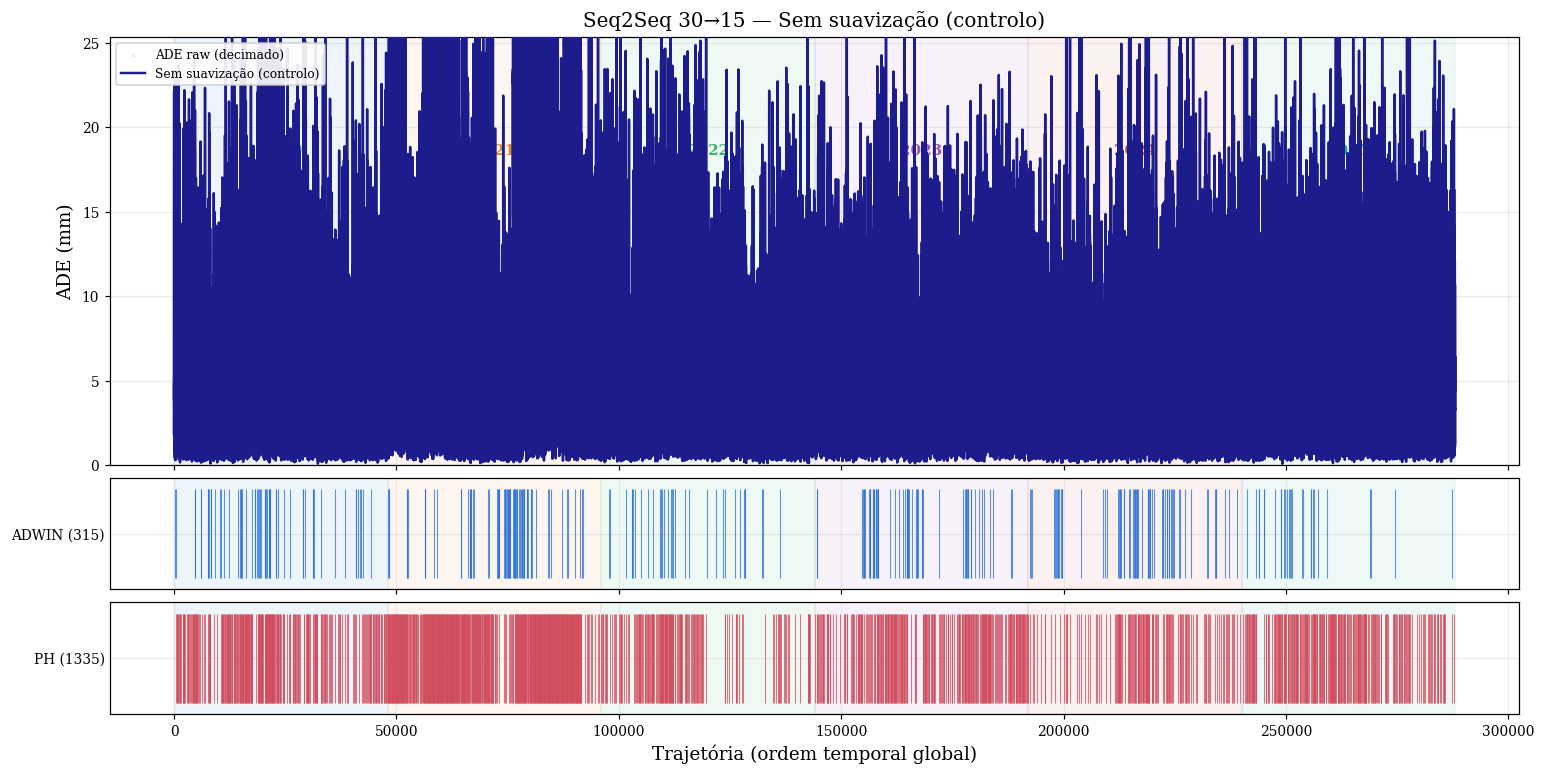
\includegraphics[width=\linewidth]{../mes9_phase1/images/ctrl/ctrl_seq2seq}
\caption{\texttt{ctrl} --- Seq2Seq.}
\end{subfigure}\hfill
\begin{subfigure}[b]{0.48\textwidth}
\centering
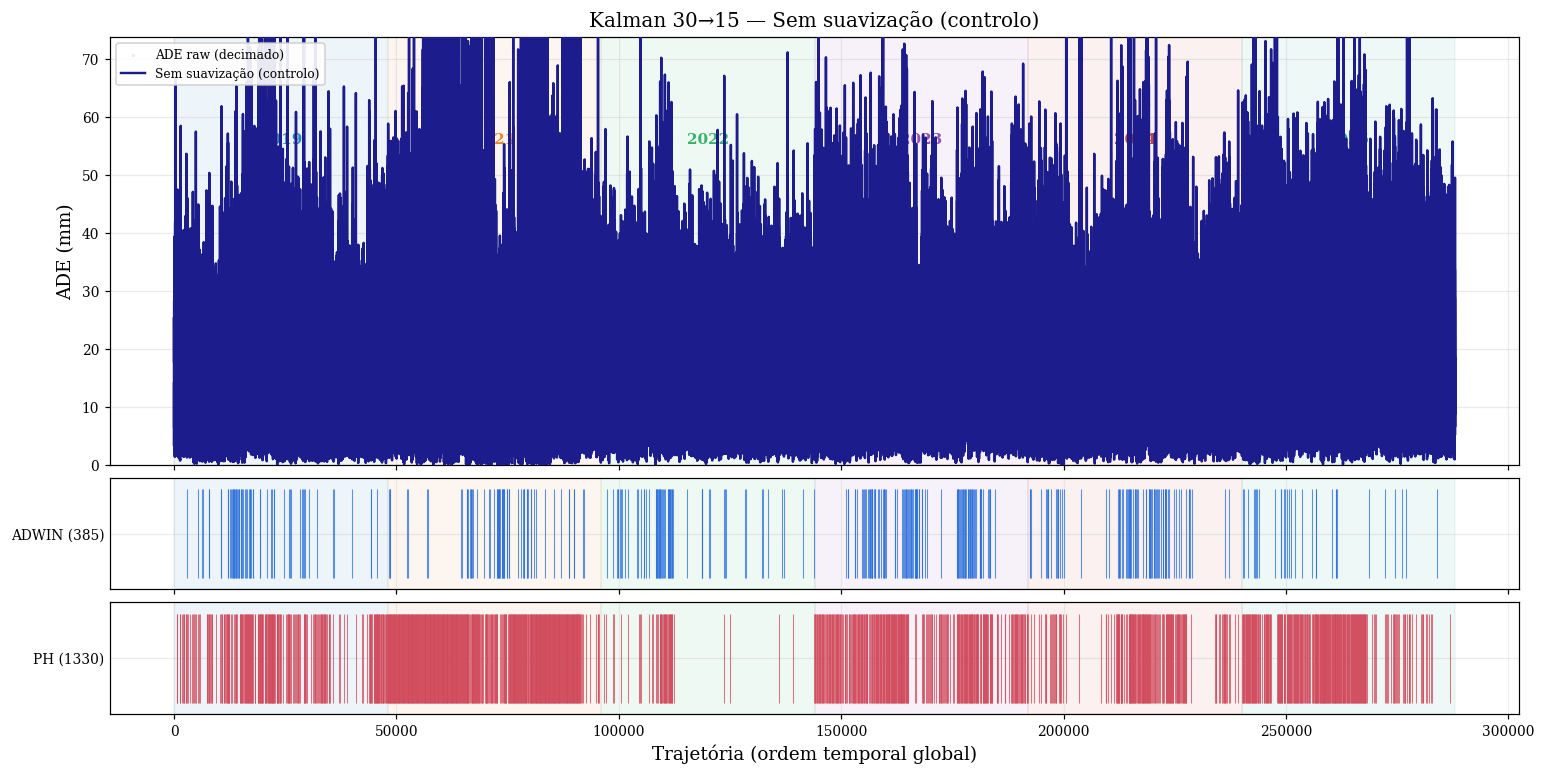
\includegraphics[width=\linewidth]{../mes9_phase1/images/ctrl/ctrl_kalman}
\caption{\texttt{ctrl} --- Kalman.}
\end{subfigure}
\caption{\textbf{Controlo (sem suaviza\c{c}\~ao).}
         FAR\textsubscript{2019} Seq2Seq: ADWIN=1{,}229/1k, PH=4{,}396/1k;
         Kalman: ADWIN=1{,}271/1k, PH=4{,}396/1k. Linha de base do
         experimento de Fase 1.}
\label{fig:m9_p1_g1}
\end{figure}

\begin{figure}[H]
\centering
\begin{subfigure}[b]{0.48\textwidth}\centering
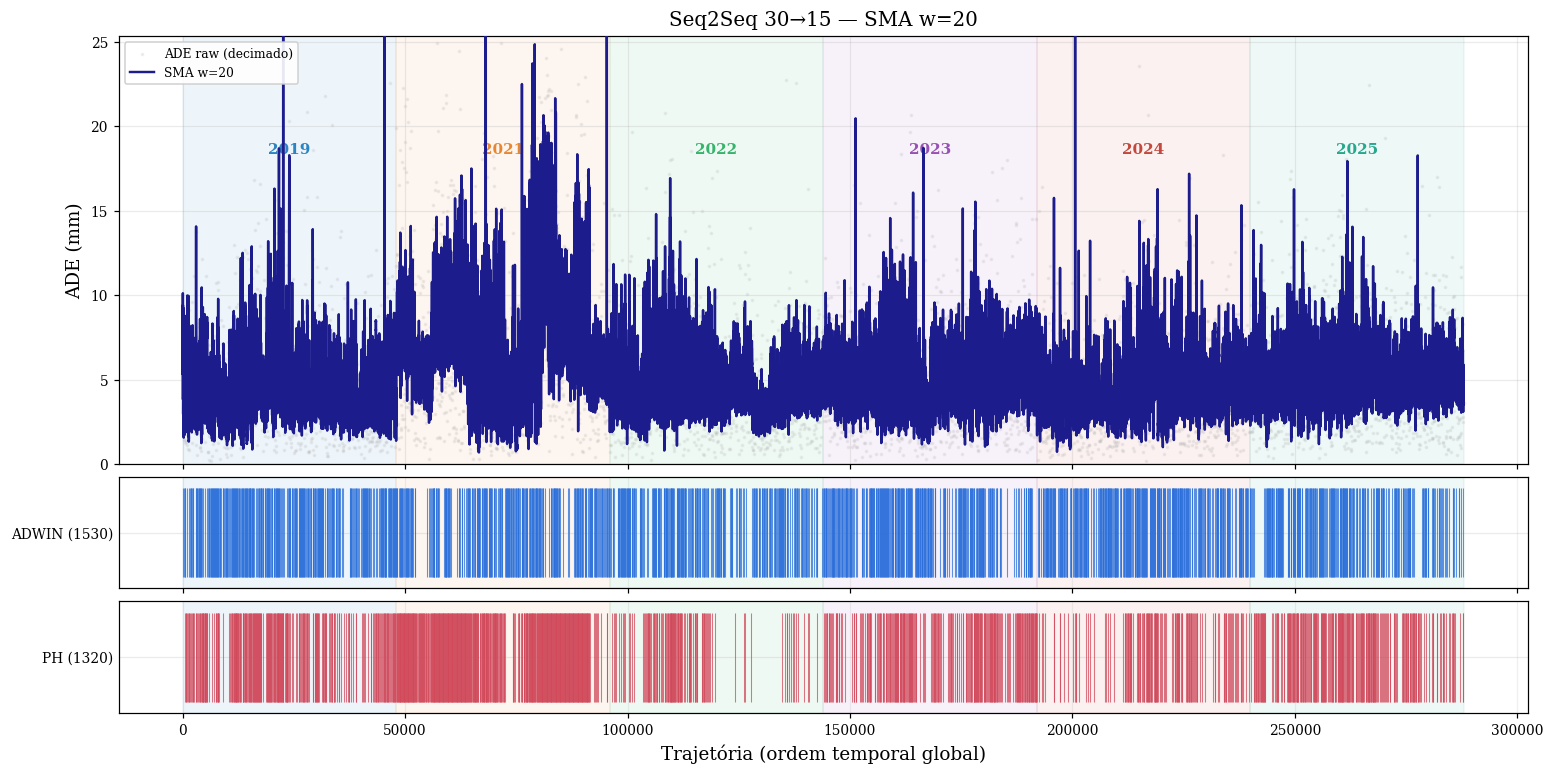
\includegraphics[width=\linewidth]{../mes9_phase1/images/sma_w020/sma_w020_seq2seq}\caption{\texttt{sma\_w020} --- S2S.}\end{subfigure}\hfill
\begin{subfigure}[b]{0.48\textwidth}\centering
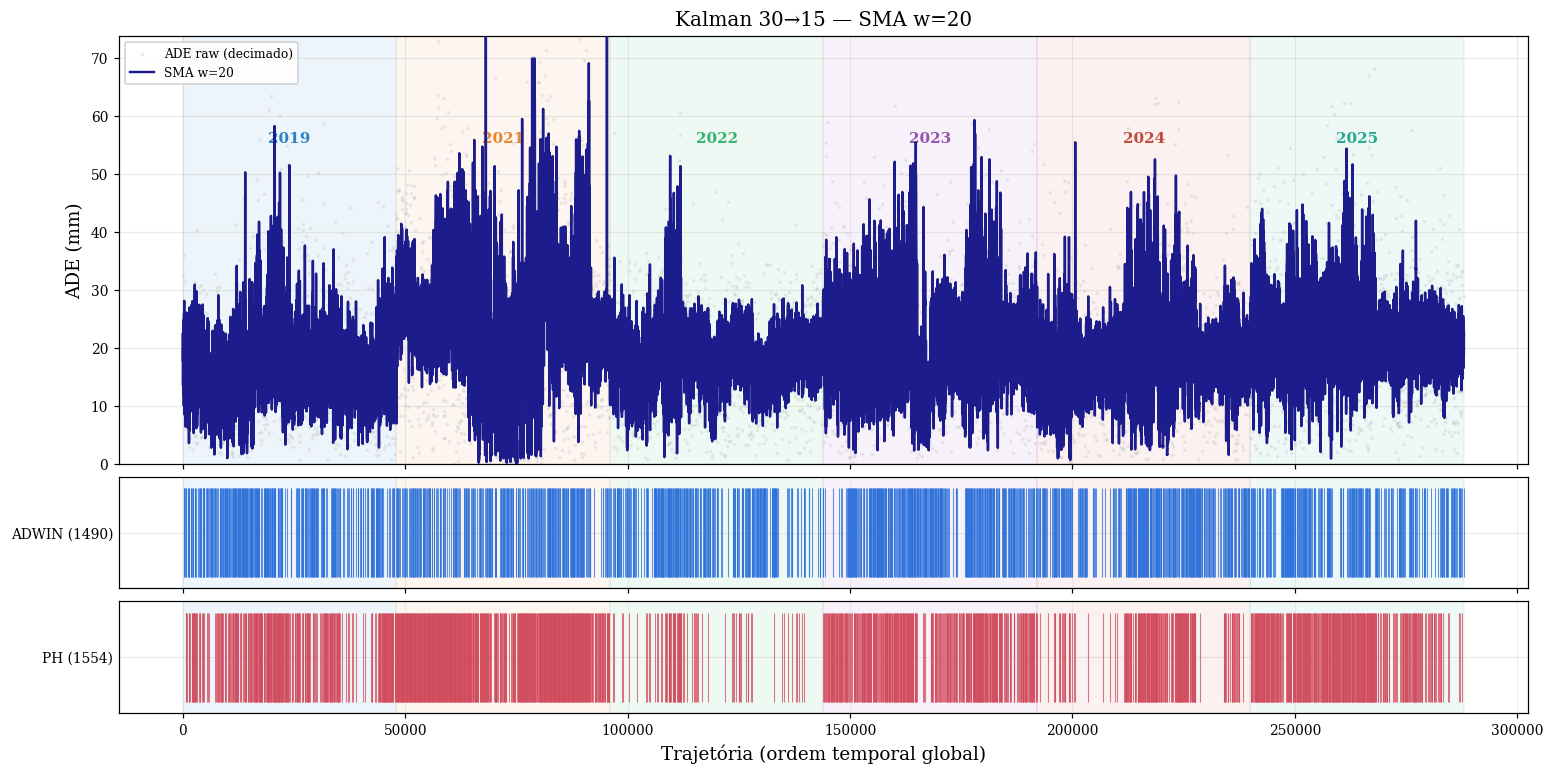
\includegraphics[width=\linewidth]{../mes9_phase1/images/sma_w020/sma_w020_kalman}\caption{\texttt{sma\_w020} --- Kalman.}\end{subfigure}

\vspace{0.3em}
\begin{subfigure}[b]{0.48\textwidth}\centering
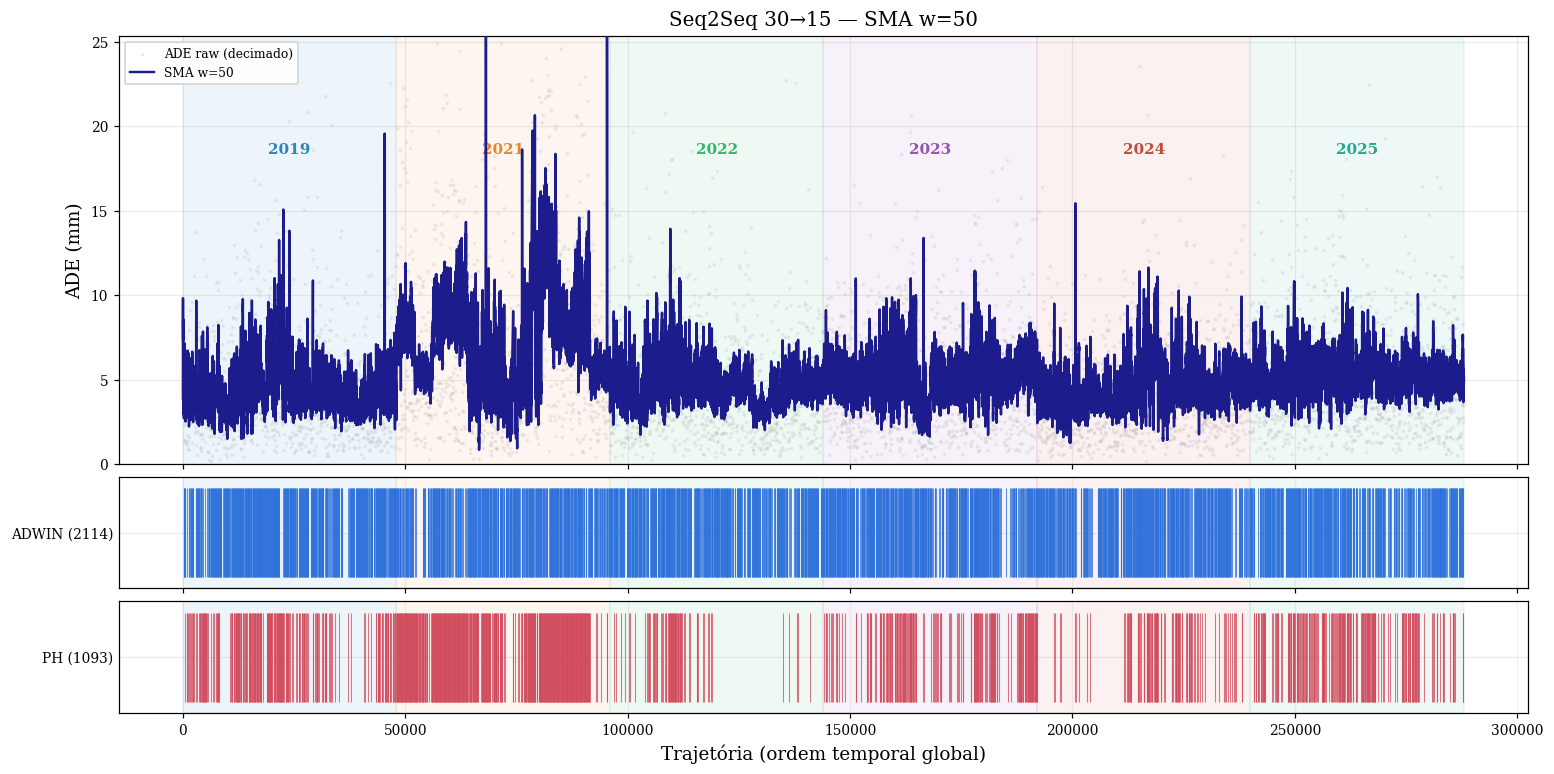
\includegraphics[width=\linewidth]{../mes9_phase1/images/sma_w050/sma_w050_seq2seq}\caption{\texttt{sma\_w050} --- S2S.}\end{subfigure}\hfill
\begin{subfigure}[b]{0.48\textwidth}\centering
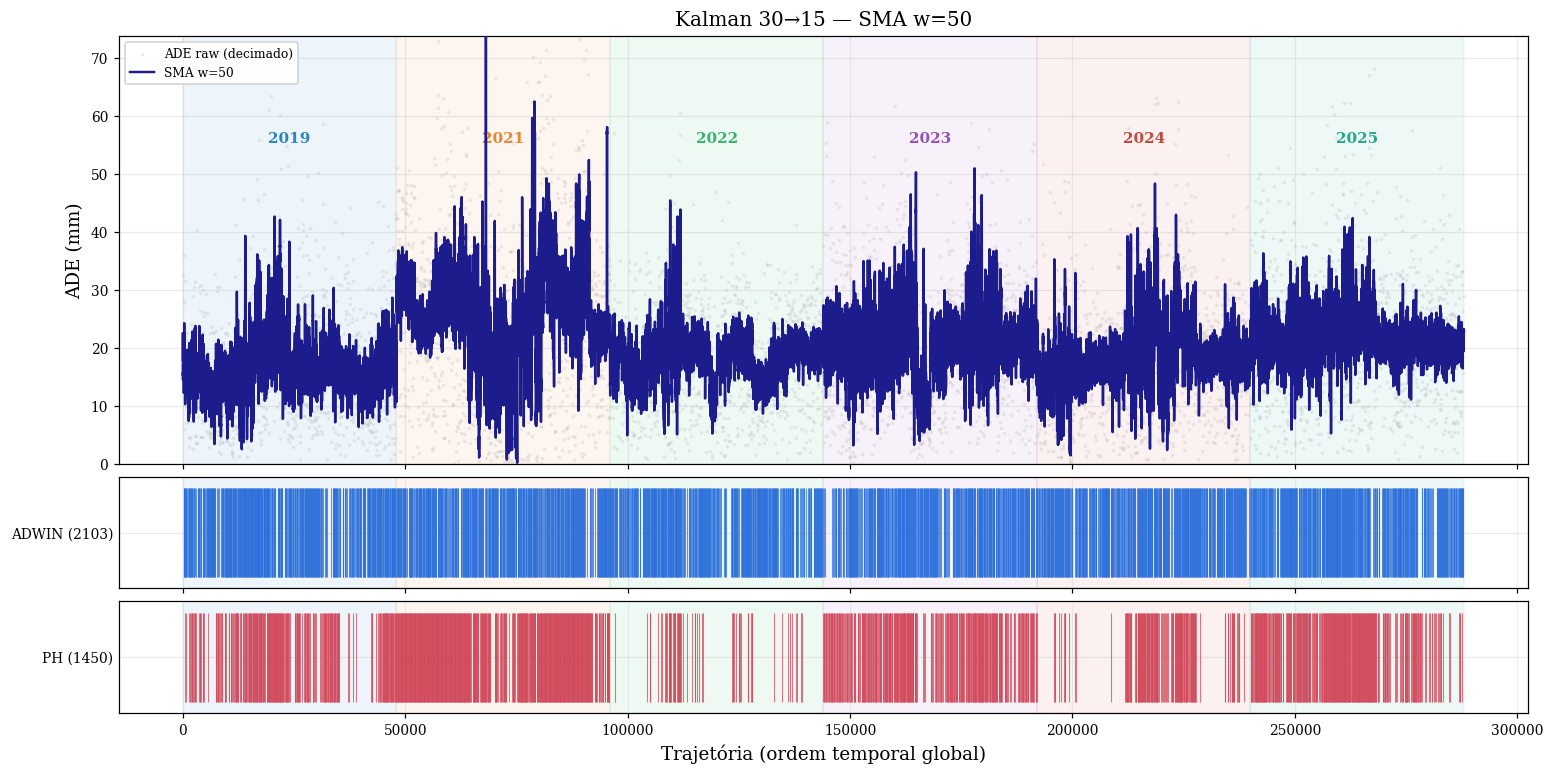
\includegraphics[width=\linewidth]{../mes9_phase1/images/sma_w050/sma_w050_kalman}\caption{\texttt{sma\_w050} --- Kalman.}\end{subfigure}
\caption{\textbf{SMA $w$=20 e $w$=50.} Suavizadores cl\'assicos n\~ao
         reduzem FAR: sob SMA $w$=20 a FAR\textsubscript{2019} sobe de
         1{,}229/1k para 5{,}917/1k no Seq2Seq (ADWIN), porque a
         redu\c{c}\~ao de vari\^ancia local satura o detector com falsos
         positivos.}
\label{fig:m9_p1_g2}
\end{figure}

\begin{figure}[H]
\centering
\begin{subfigure}[b]{0.48\textwidth}\centering
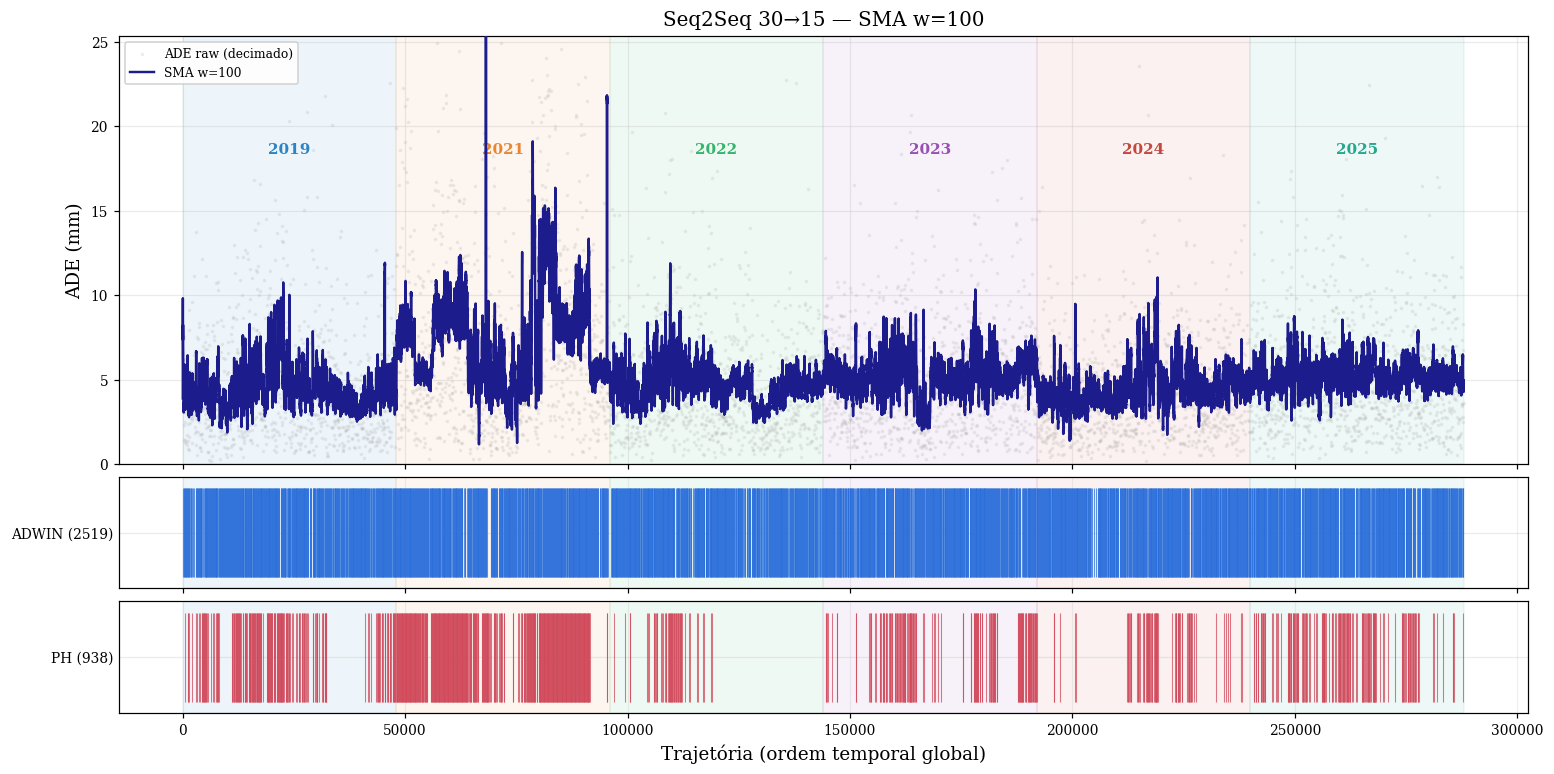
\includegraphics[width=\linewidth]{../mes9_phase1/images/sma_w100/sma_w100_seq2seq}\caption{\texttt{sma\_w100} --- S2S.}\end{subfigure}\hfill
\begin{subfigure}[b]{0.48\textwidth}\centering
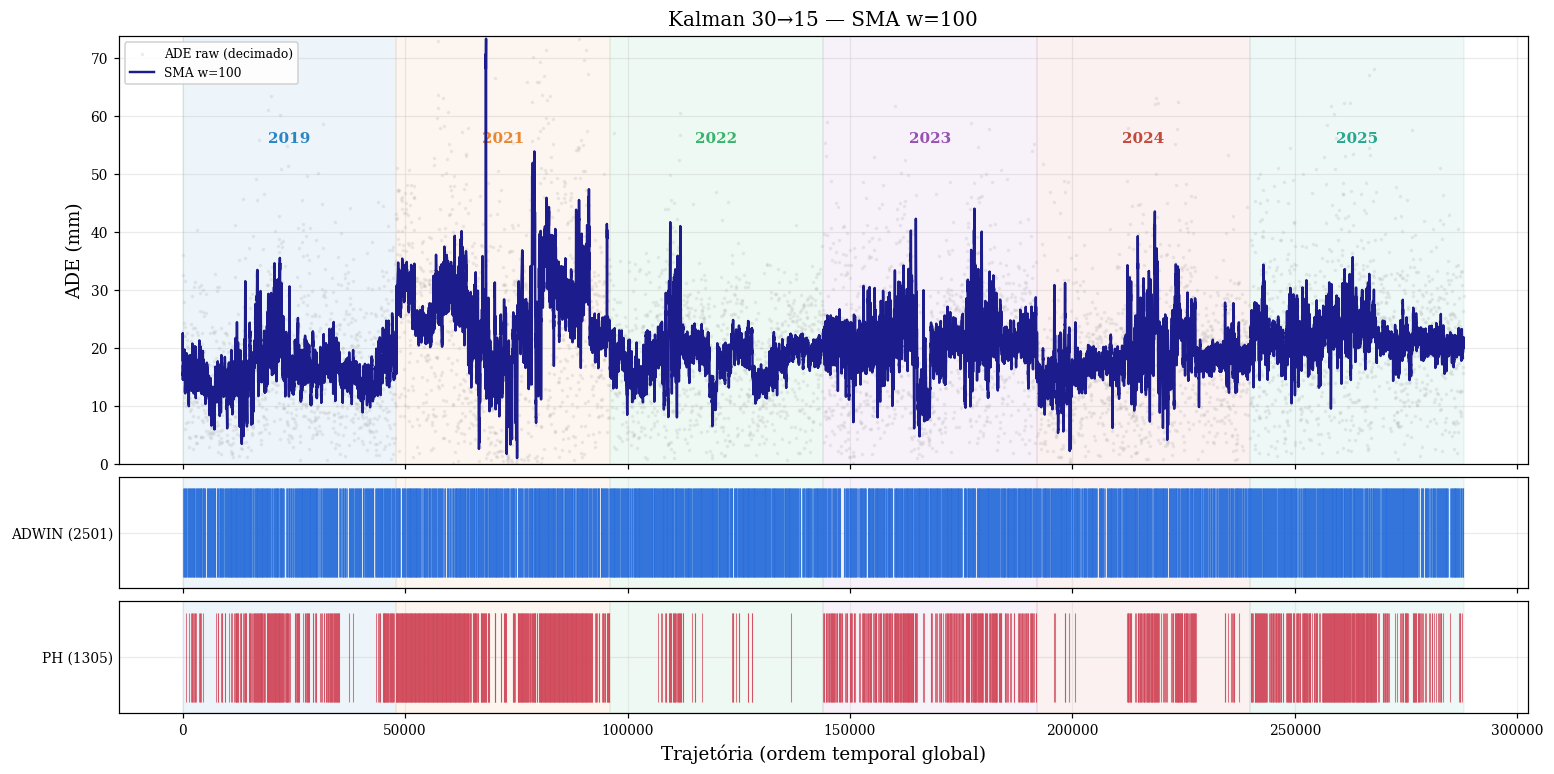
\includegraphics[width=\linewidth]{../mes9_phase1/images/sma_w100/sma_w100_kalman}\caption{\texttt{sma\_w100} --- Kalman.}\end{subfigure}

\vspace{0.3em}
\begin{subfigure}[b]{0.48\textwidth}\centering
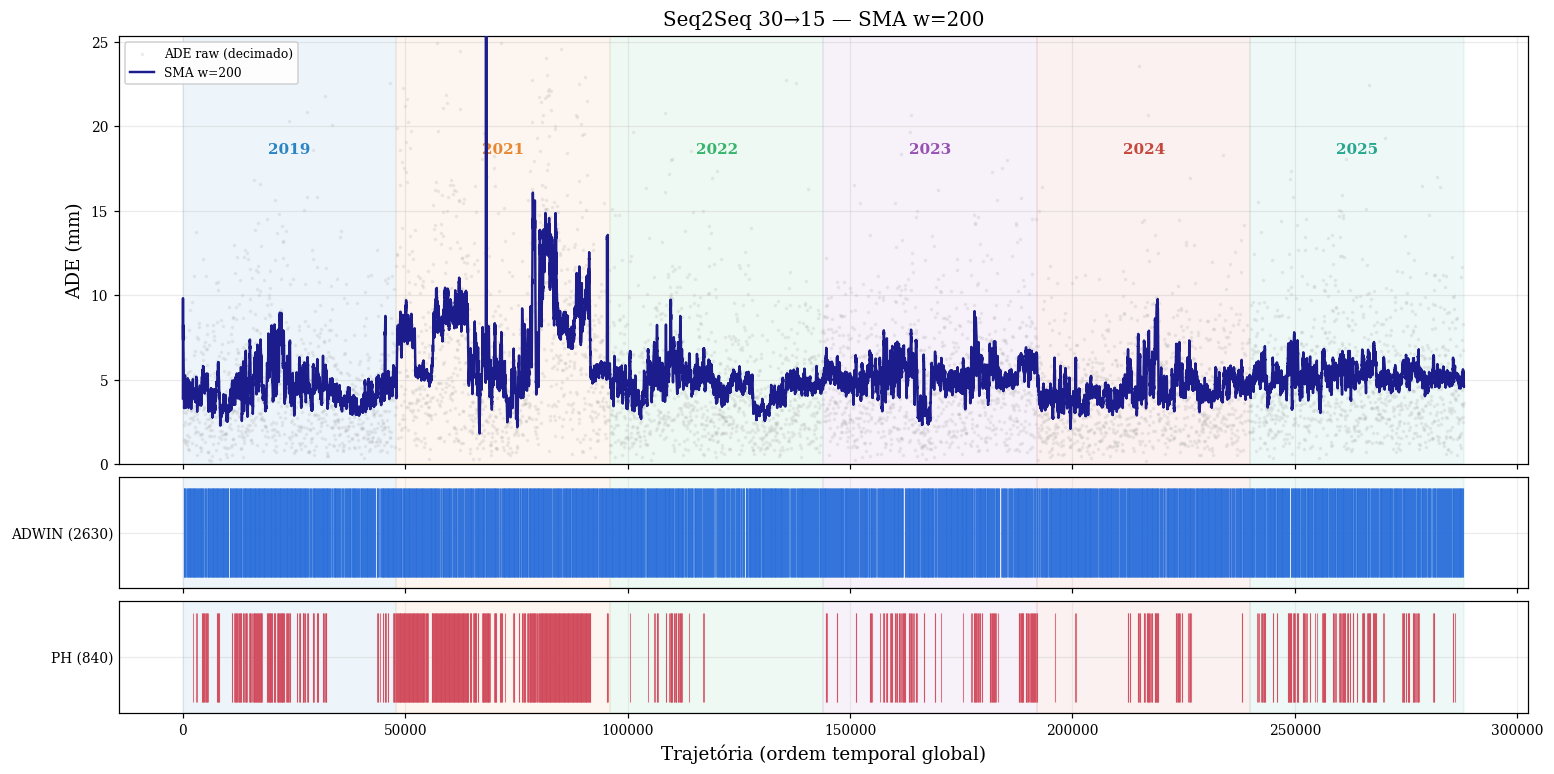
\includegraphics[width=\linewidth]{../mes9_phase1/images/sma_w200/sma_w200_seq2seq}\caption{\texttt{sma\_w200} --- S2S.}\end{subfigure}\hfill
\begin{subfigure}[b]{0.48\textwidth}\centering
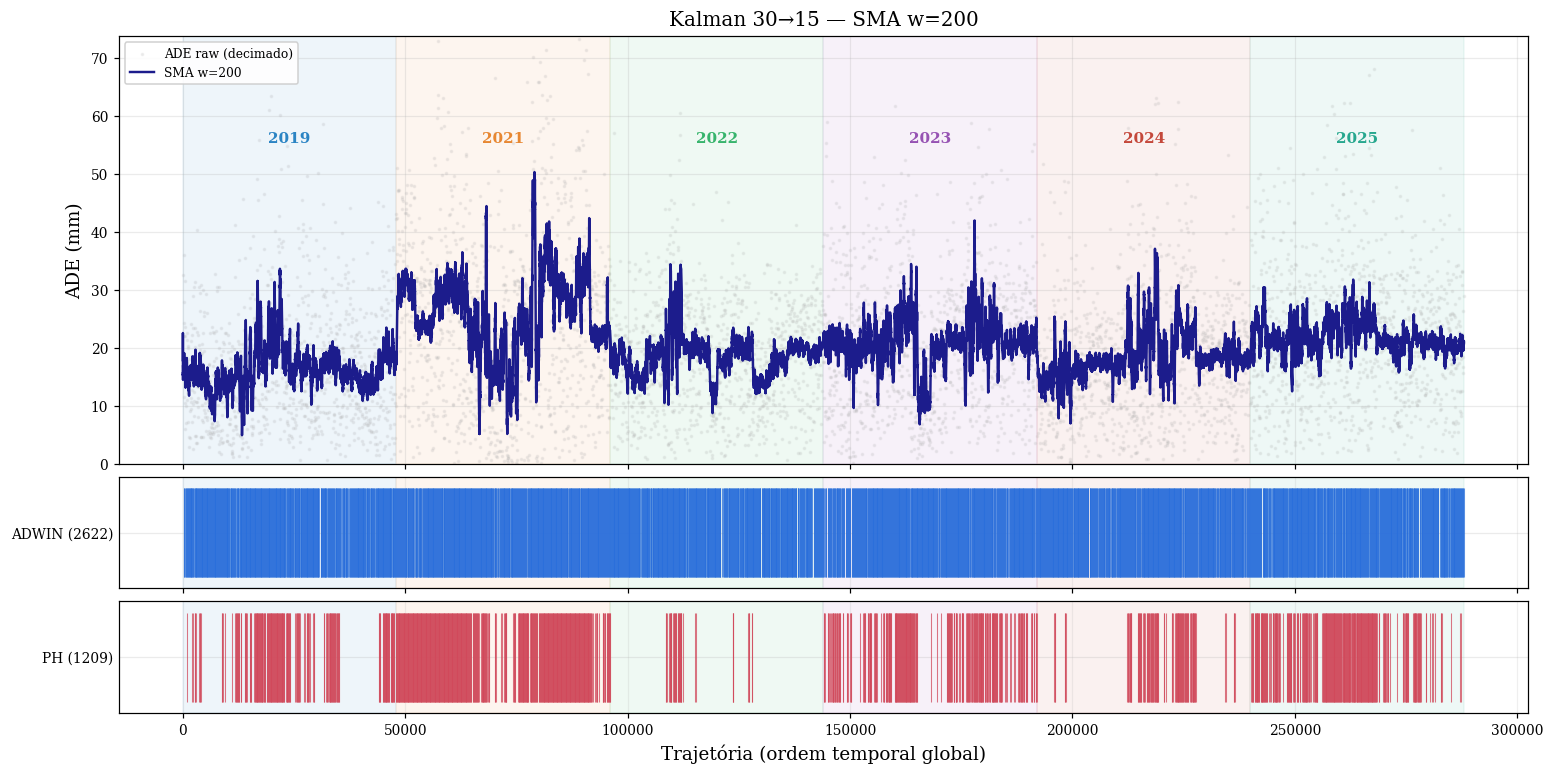
\includegraphics[width=\linewidth]{../mes9_phase1/images/sma_w200/sma_w200_kalman}\caption{\texttt{sma\_w200} --- Kalman.}\end{subfigure}
\caption{\textbf{SMA $w$=100 e $w$=200.} Janelas maiores tornam o sinal
         mais ``r\'igido'' e geram mais alarmes ainda --- o ADWIN
         reage \`a discrep\^ancia entre o sinal achatado e a variabilidade
         intr\'inseca da janela operacional.}
\label{fig:m9_p1_g3}
\end{figure}

\begin{figure}[H]
\centering
\begin{subfigure}[b]{0.48\textwidth}\centering
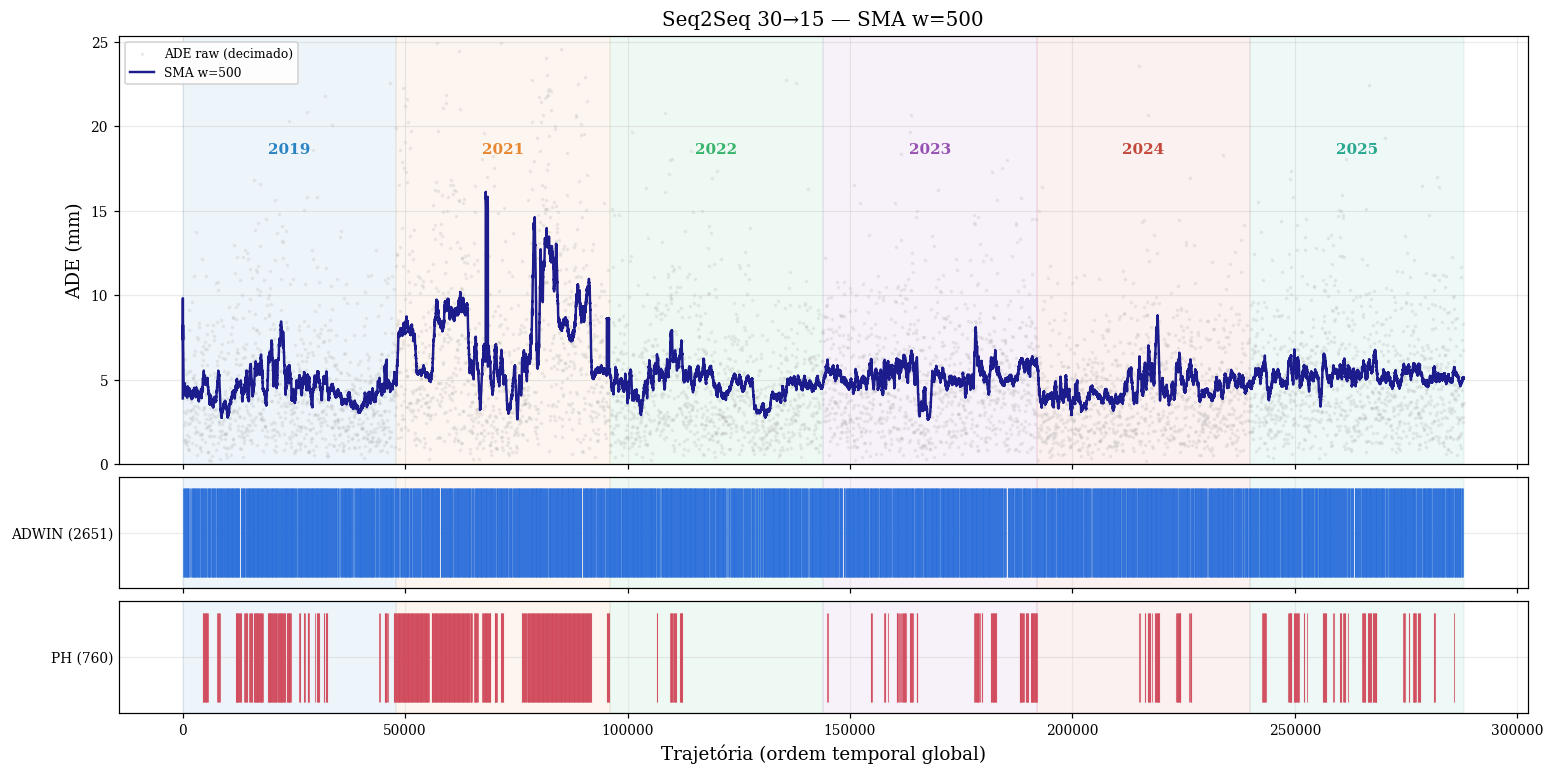
\includegraphics[width=\linewidth]{../mes9_phase1/images/sma_w500/sma_w500_seq2seq}\caption{\texttt{sma\_w500} --- S2S.}\end{subfigure}\hfill
\begin{subfigure}[b]{0.48\textwidth}\centering
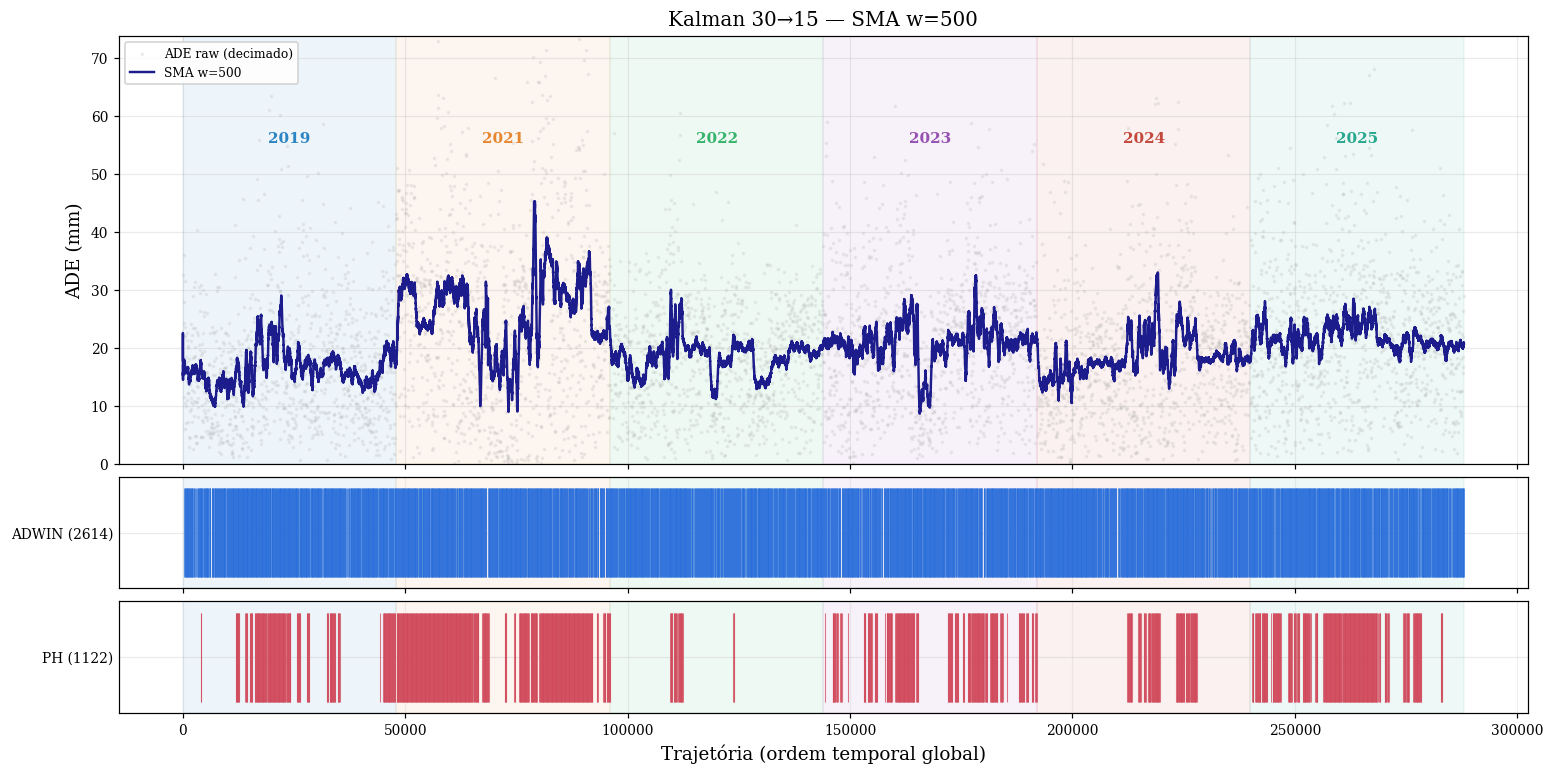
\includegraphics[width=\linewidth]{../mes9_phase1/images/sma_w500/sma_w500_kalman}\caption{\texttt{sma\_w500} --- Kalman.}\end{subfigure}

\vspace{0.3em}
\begin{subfigure}[b]{0.48\textwidth}\centering
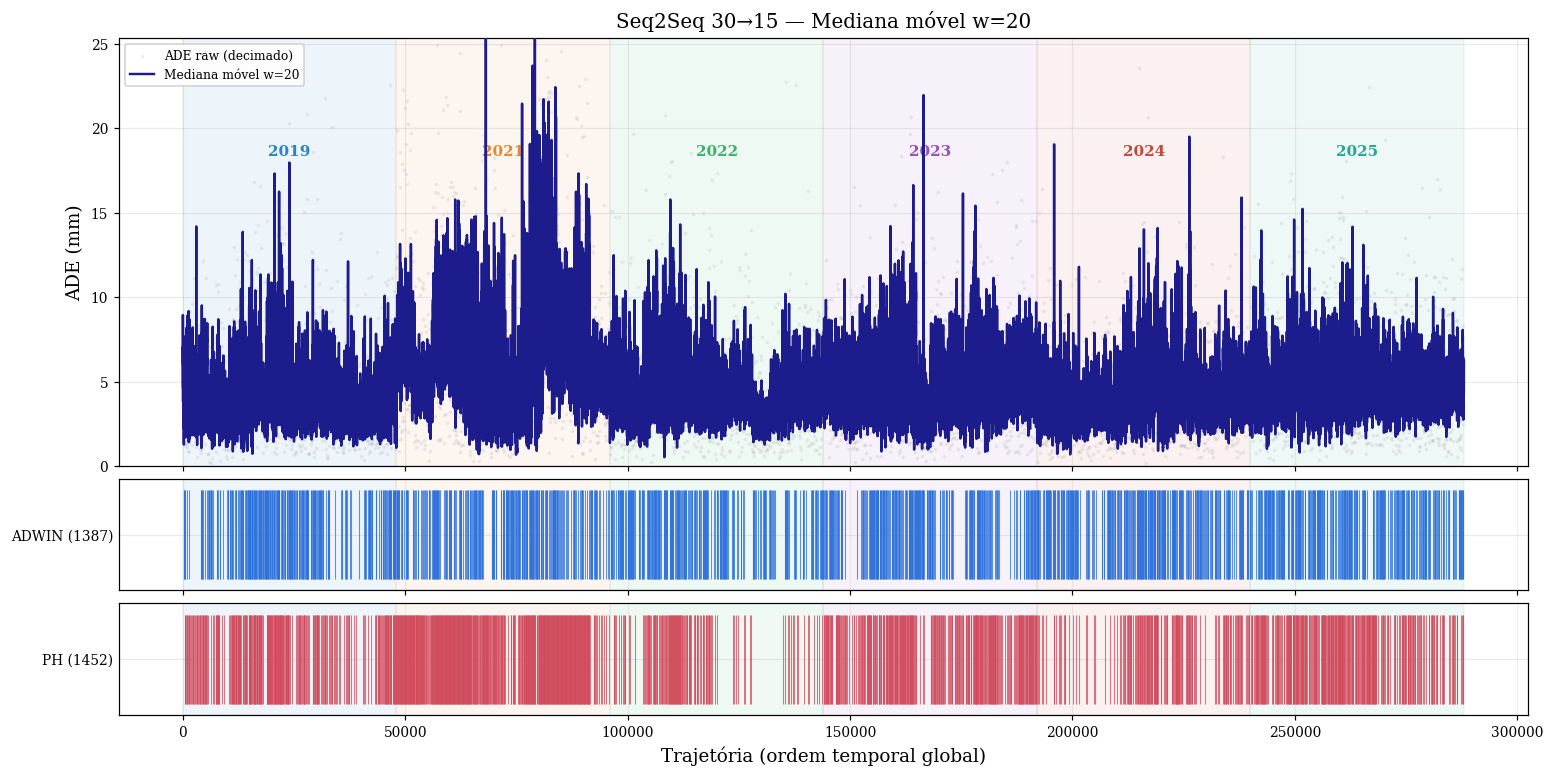
\includegraphics[width=\linewidth]{../mes9_phase1/images/med_w020/med_w020_seq2seq}\caption{\texttt{med\_w020} --- S2S.}\end{subfigure}\hfill
\begin{subfigure}[b]{0.48\textwidth}\centering
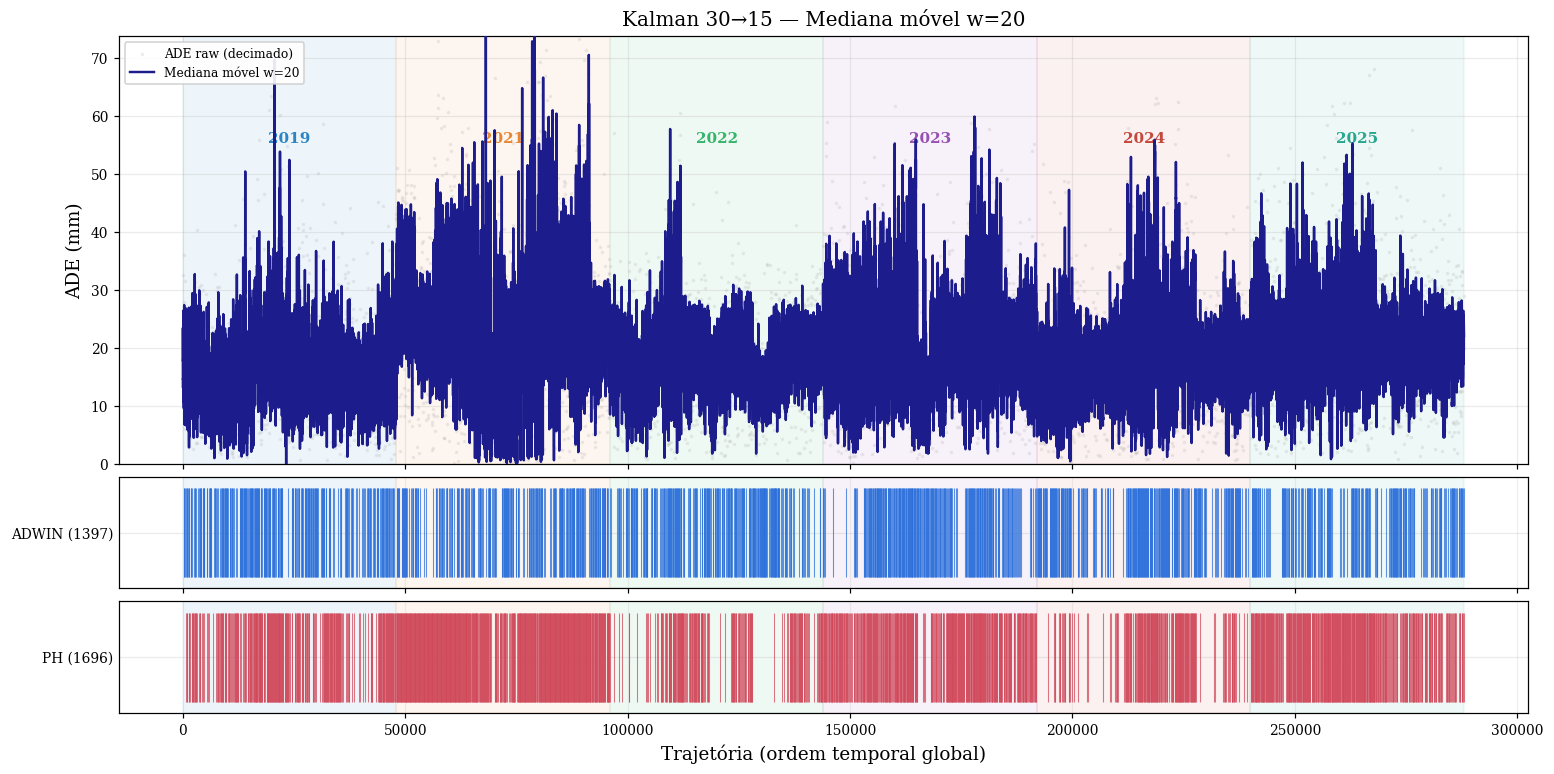
\includegraphics[width=\linewidth]{../mes9_phase1/images/med_w020/med_w020_kalman}\caption{\texttt{med\_w020} --- Kalman.}\end{subfigure}
\caption{\textbf{SMA $w$=500 e Mediana $w$=20.} A mediana m\'ovel tem
         comportamento qualitativamente similar \`a SMA --- ambas
         saturam o ADWIN com pseudo-alarmes na transi\c{c}\~ao
         2019$\to$2021.}
\label{fig:m9_p1_g4}
\end{figure}

\begin{figure}[H]
\centering
\begin{subfigure}[b]{0.48\textwidth}\centering
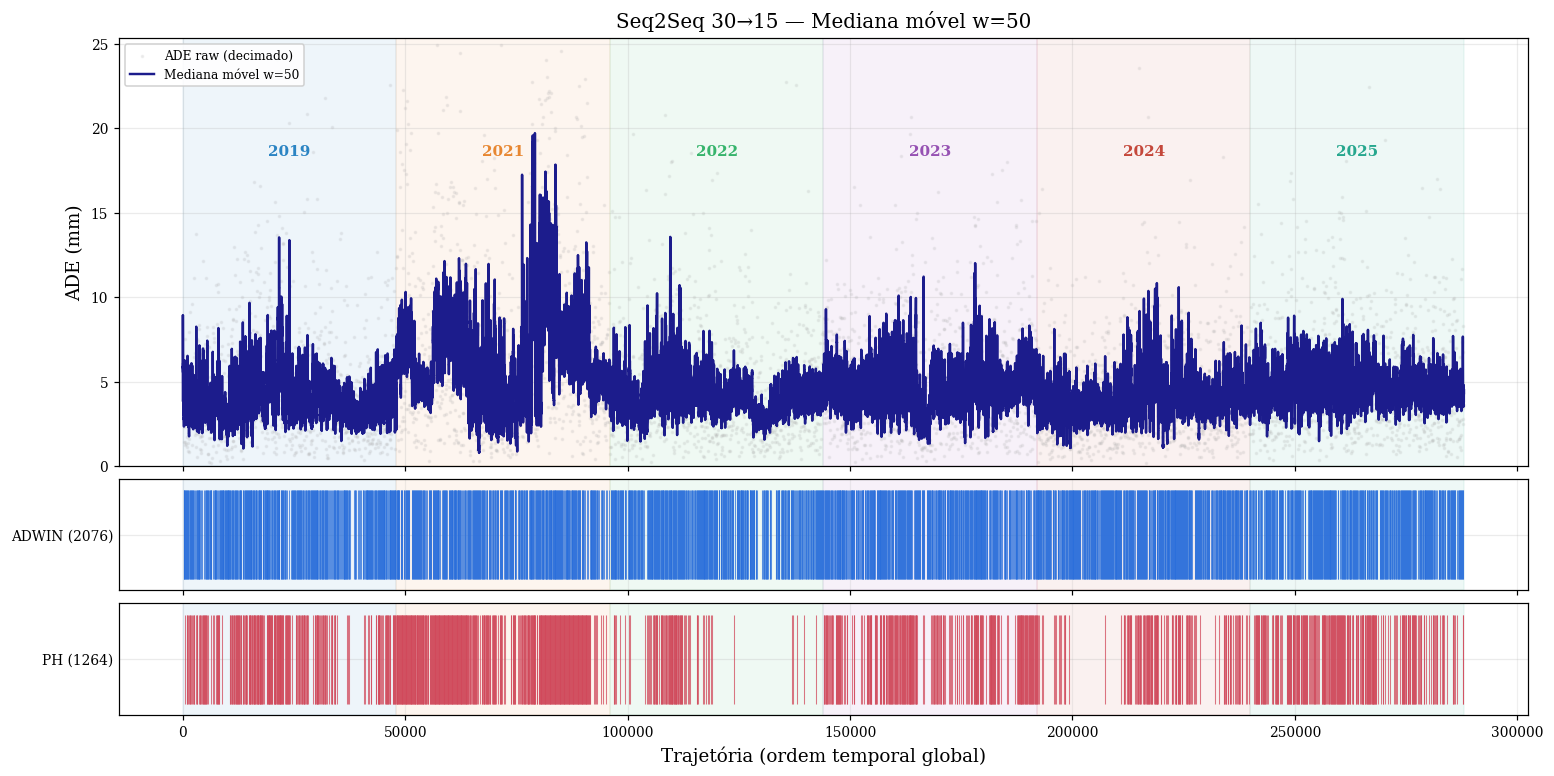
\includegraphics[width=\linewidth]{../mes9_phase1/images/med_w050/med_w050_seq2seq}\caption{\texttt{med\_w050} --- S2S.}\end{subfigure}\hfill
\begin{subfigure}[b]{0.48\textwidth}\centering
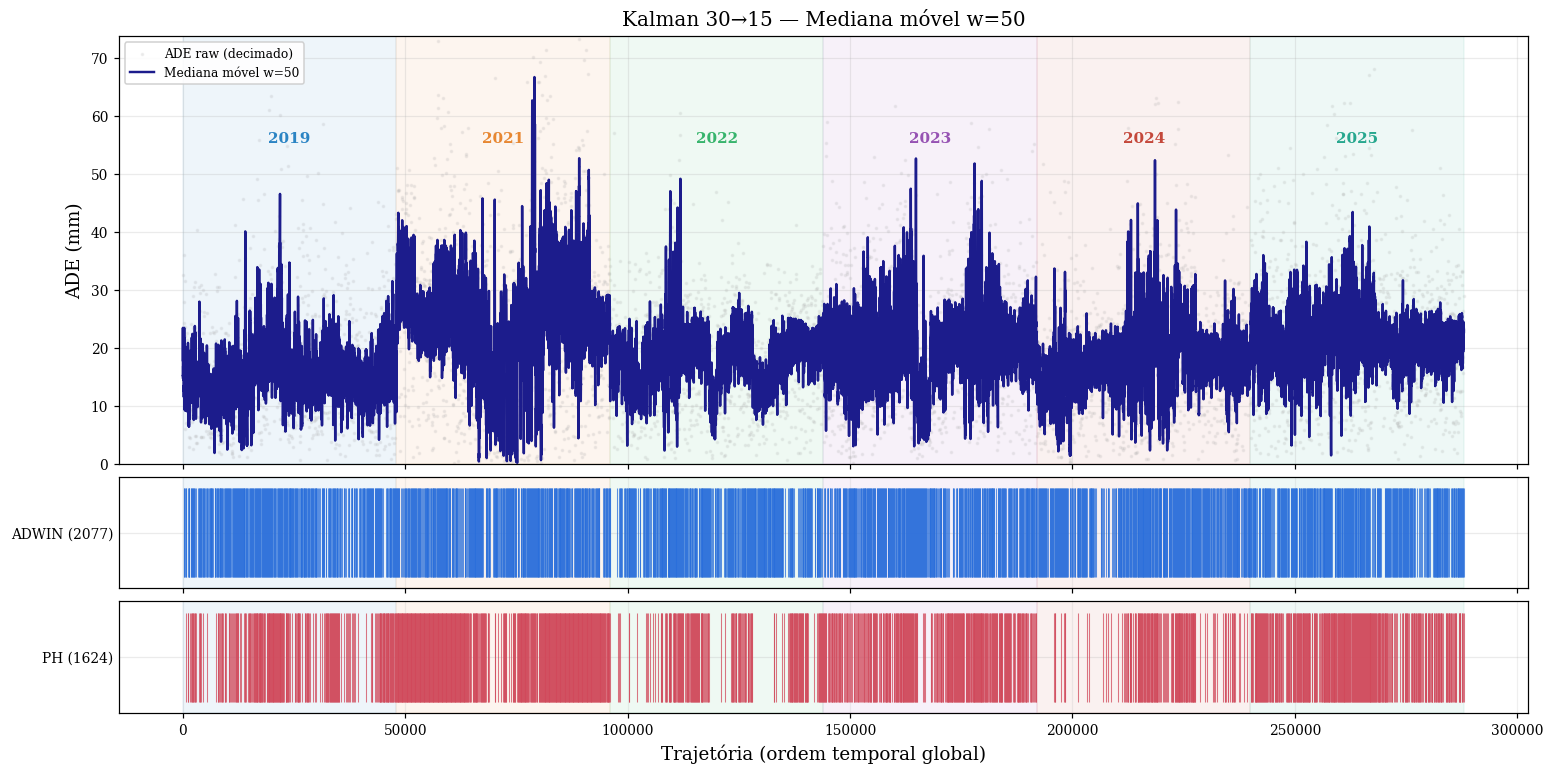
\includegraphics[width=\linewidth]{../mes9_phase1/images/med_w050/med_w050_kalman}\caption{\texttt{med\_w050} --- Kalman.}\end{subfigure}

\vspace{0.3em}
\begin{subfigure}[b]{0.48\textwidth}\centering
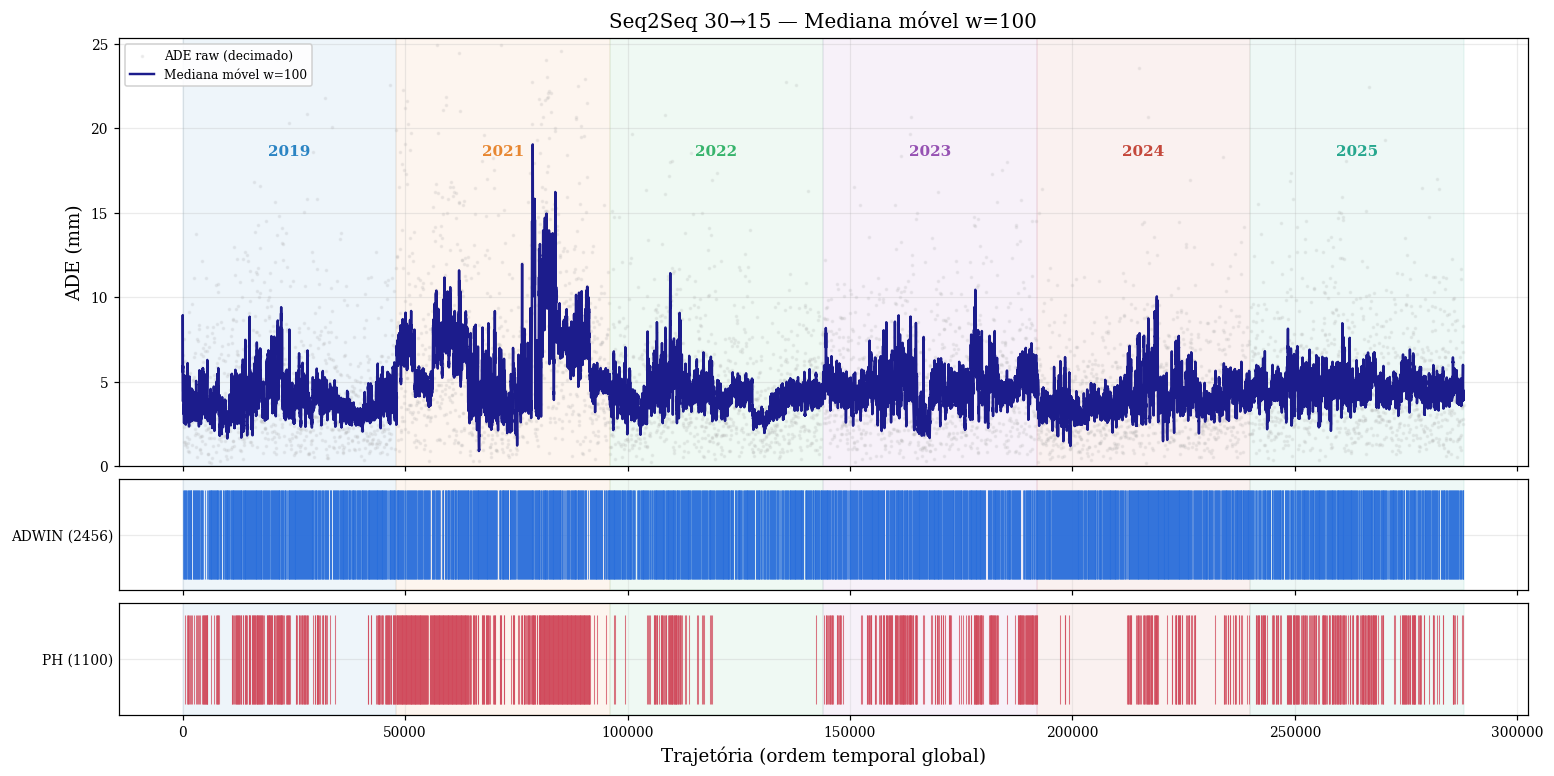
\includegraphics[width=\linewidth]{../mes9_phase1/images/med_w100/med_w100_seq2seq}\caption{\texttt{med\_w100} --- S2S.}\end{subfigure}\hfill
\begin{subfigure}[b]{0.48\textwidth}\centering
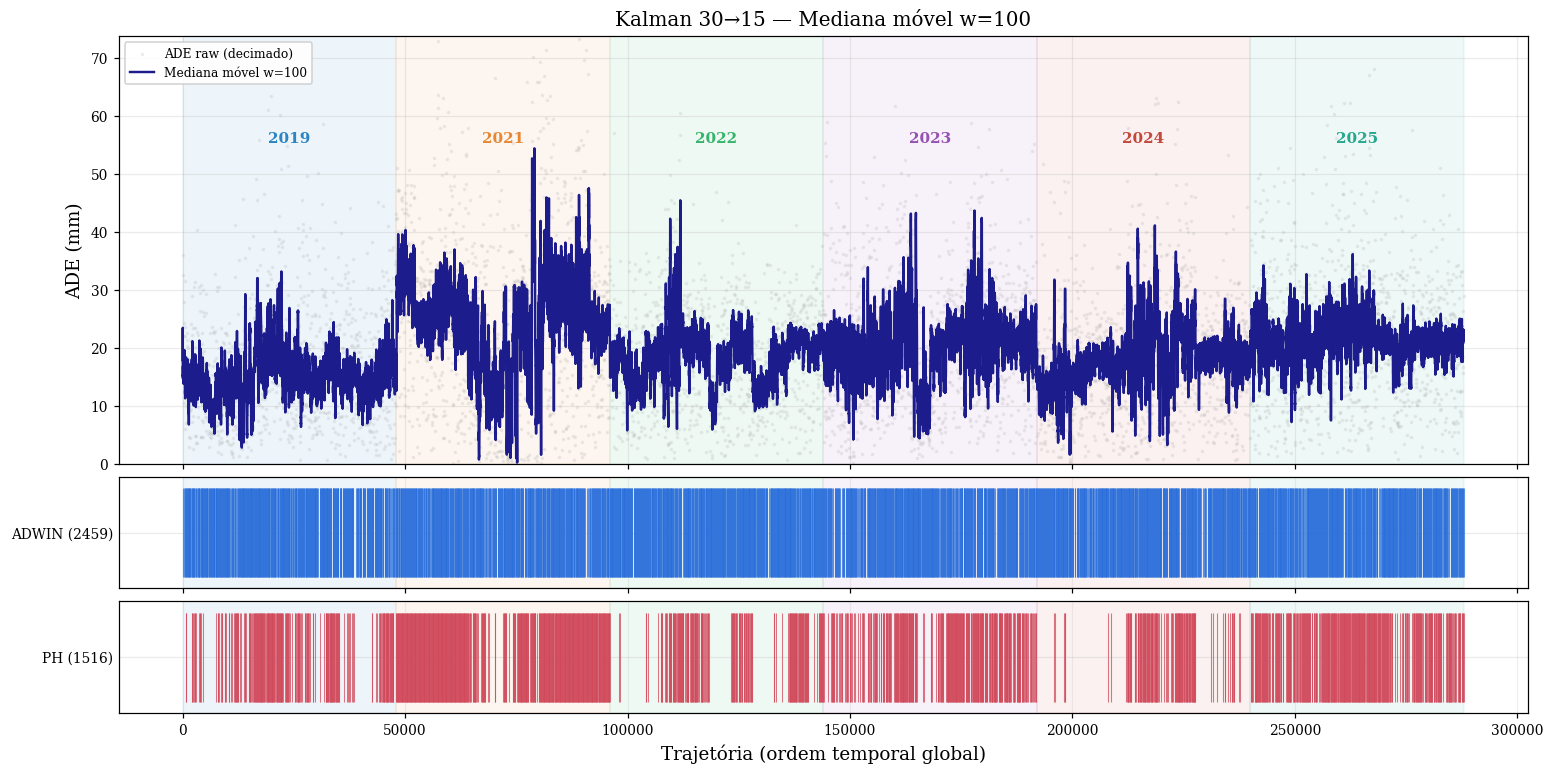
\includegraphics[width=\linewidth]{../mes9_phase1/images/med_w100/med_w100_kalman}\caption{\texttt{med\_w100} --- Kalman.}\end{subfigure}
\caption{\textbf{Mediana $w$=50 e $w$=100.}}
\label{fig:m9_p1_g5}
\end{figure}

\begin{figure}[H]
\centering
\begin{subfigure}[b]{0.48\textwidth}\centering
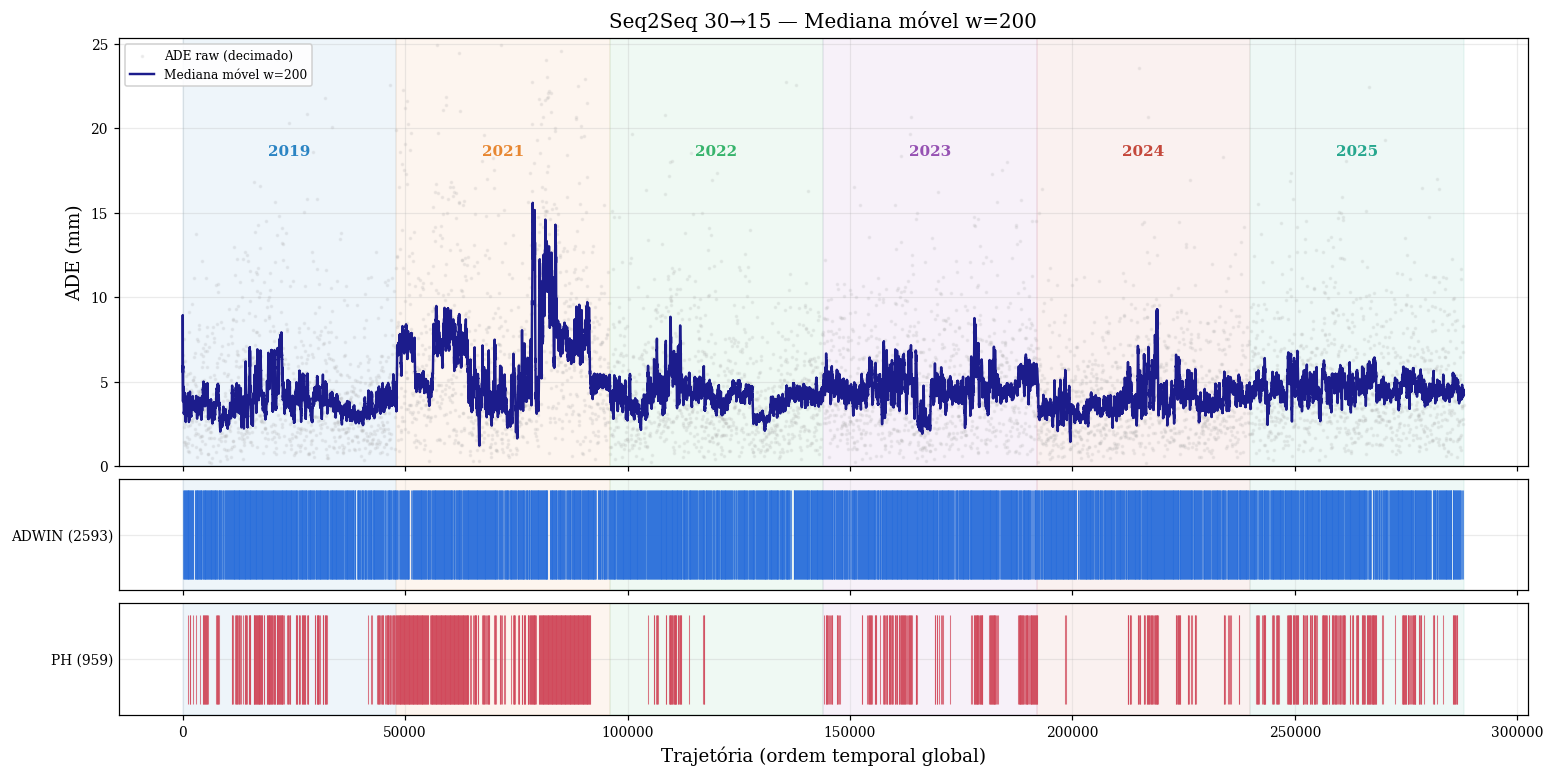
\includegraphics[width=\linewidth]{../mes9_phase1/images/med_w200/med_w200_seq2seq}\caption{\texttt{med\_w200} --- S2S.}\end{subfigure}\hfill
\begin{subfigure}[b]{0.48\textwidth}\centering
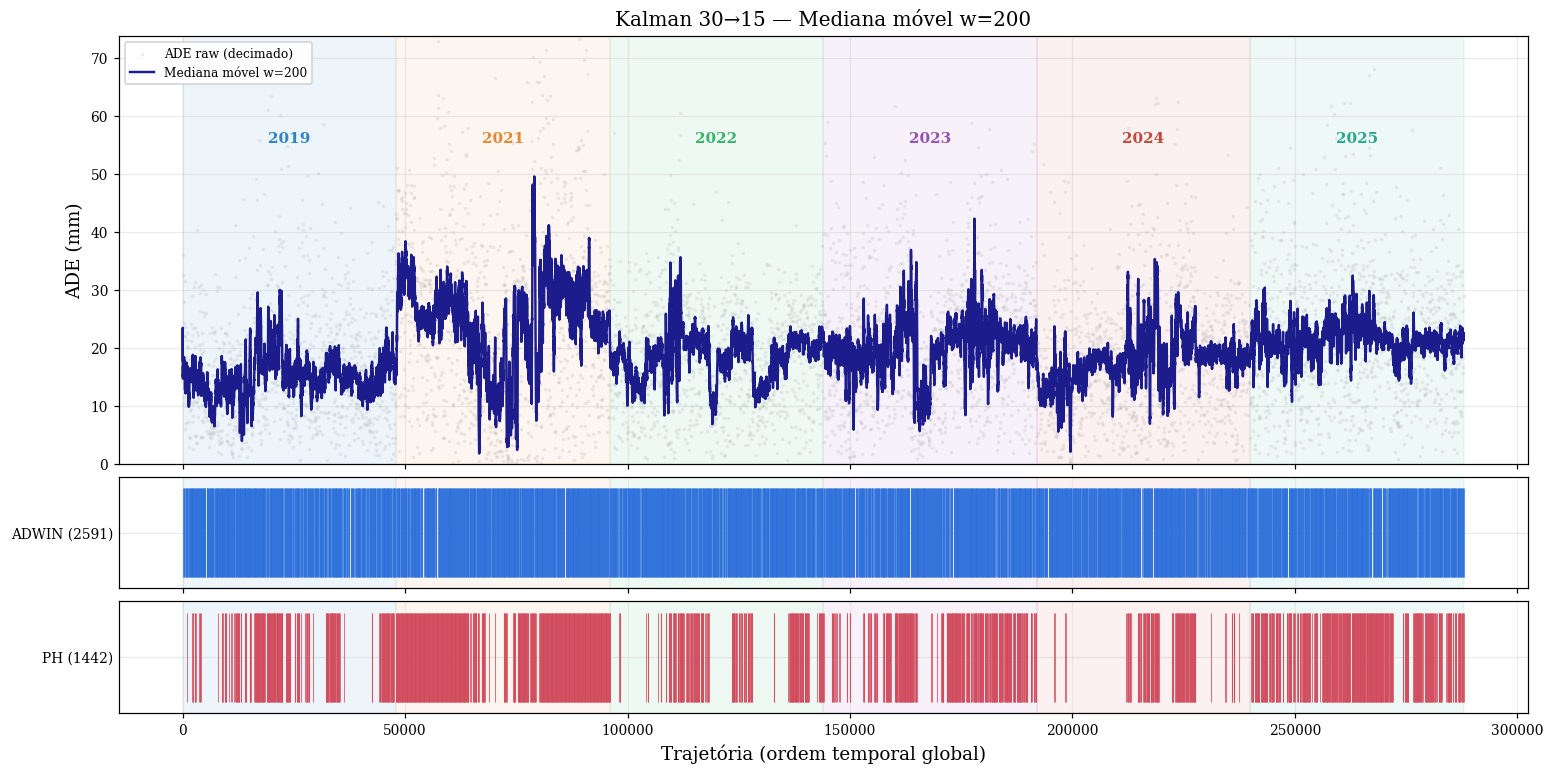
\includegraphics[width=\linewidth]{../mes9_phase1/images/med_w200/med_w200_kalman}\caption{\texttt{med\_w200} --- Kalman.}\end{subfigure}

\vspace{0.3em}
\begin{subfigure}[b]{0.48\textwidth}\centering
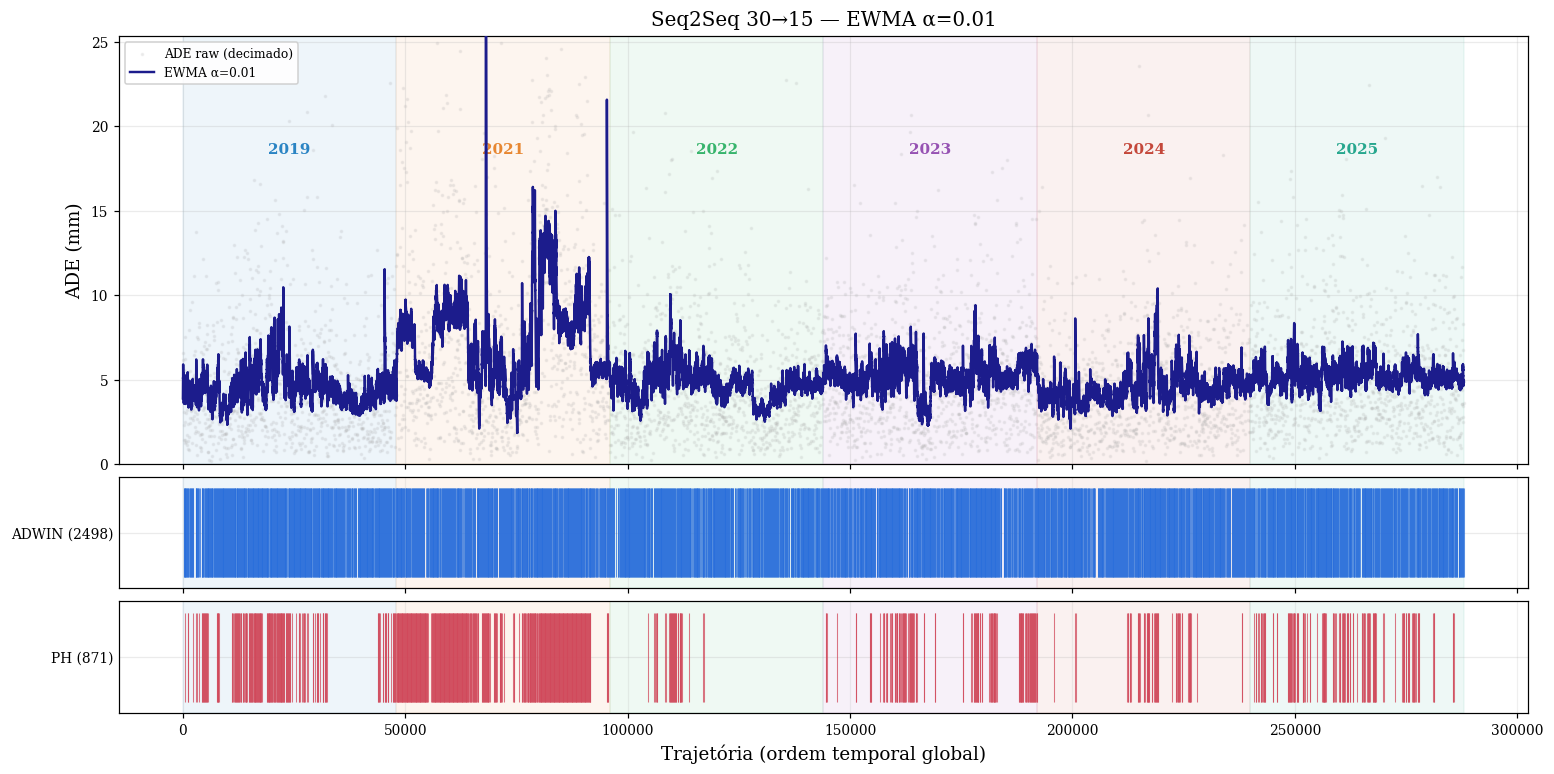
\includegraphics[width=\linewidth]{../mes9_phase1/images/ewma_a001/ewma_a001_seq2seq}\caption{\texttt{ewma\_a001} --- S2S.}\end{subfigure}\hfill
\begin{subfigure}[b]{0.48\textwidth}\centering
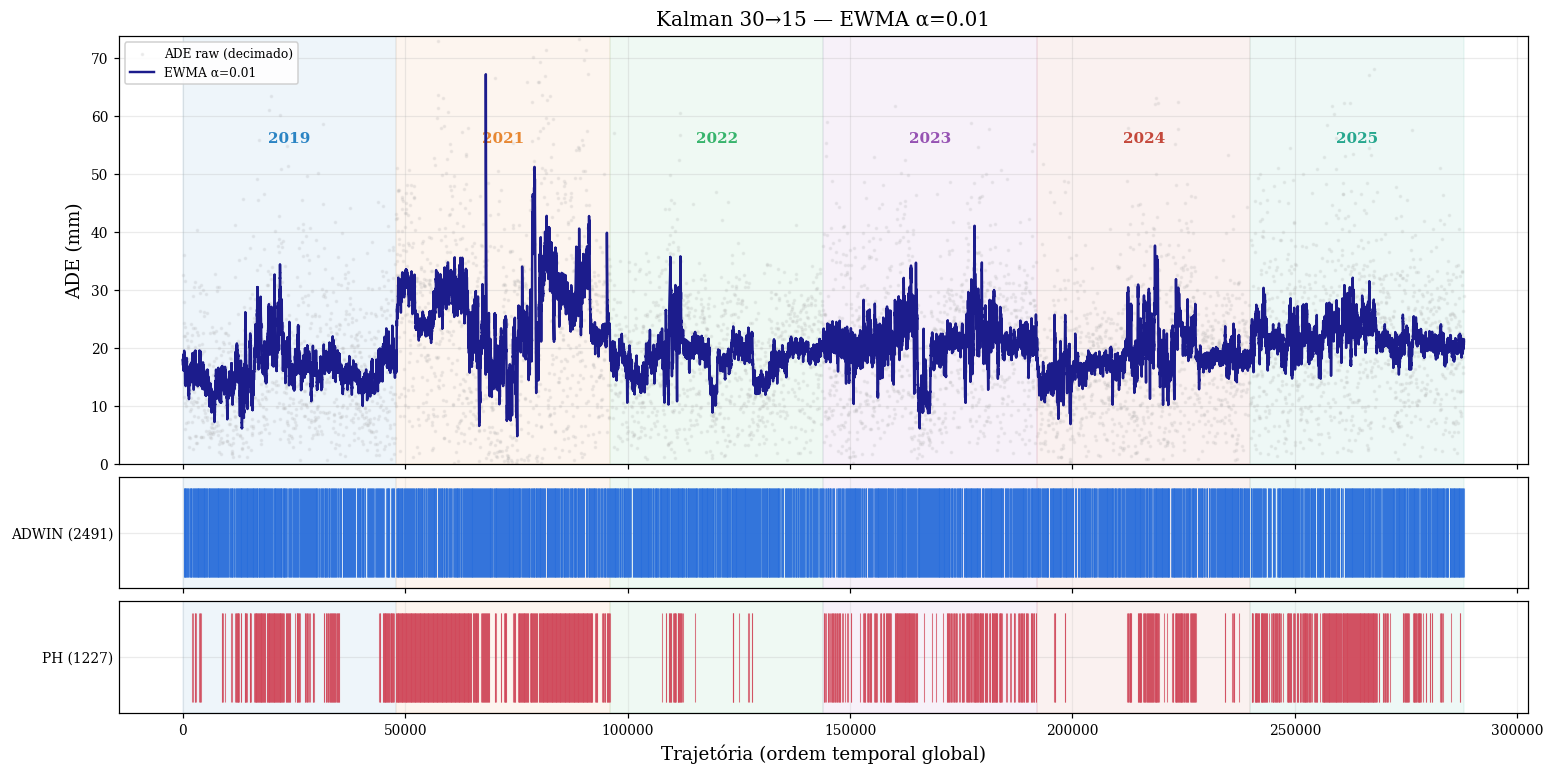
\includegraphics[width=\linewidth]{../mes9_phase1/images/ewma_a001/ewma_a001_kalman}\caption{\texttt{ewma\_a001} --- Kalman.}\end{subfigure}
\caption{\textbf{Mediana $w$=200 e EWMA $\alpha$=0{,}01.}}
\label{fig:m9_p1_g6}
\end{figure}

\begin{figure}[H]
\centering
\begin{subfigure}[b]{0.48\textwidth}\centering
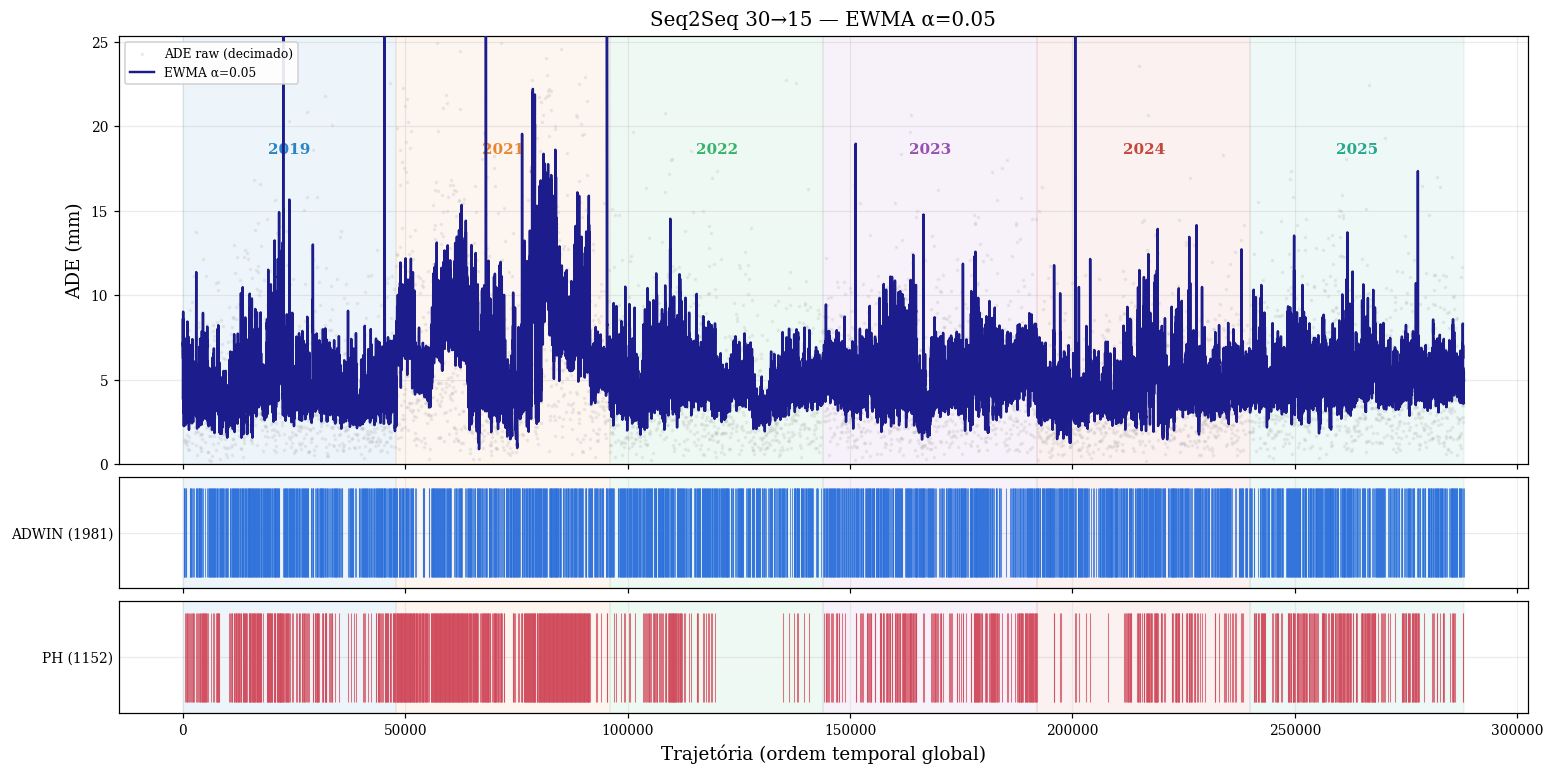
\includegraphics[width=\linewidth]{../mes9_phase1/images/ewma_a005/ewma_a005_seq2seq}\caption{\texttt{ewma\_a005} --- S2S.}\end{subfigure}\hfill
\begin{subfigure}[b]{0.48\textwidth}\centering
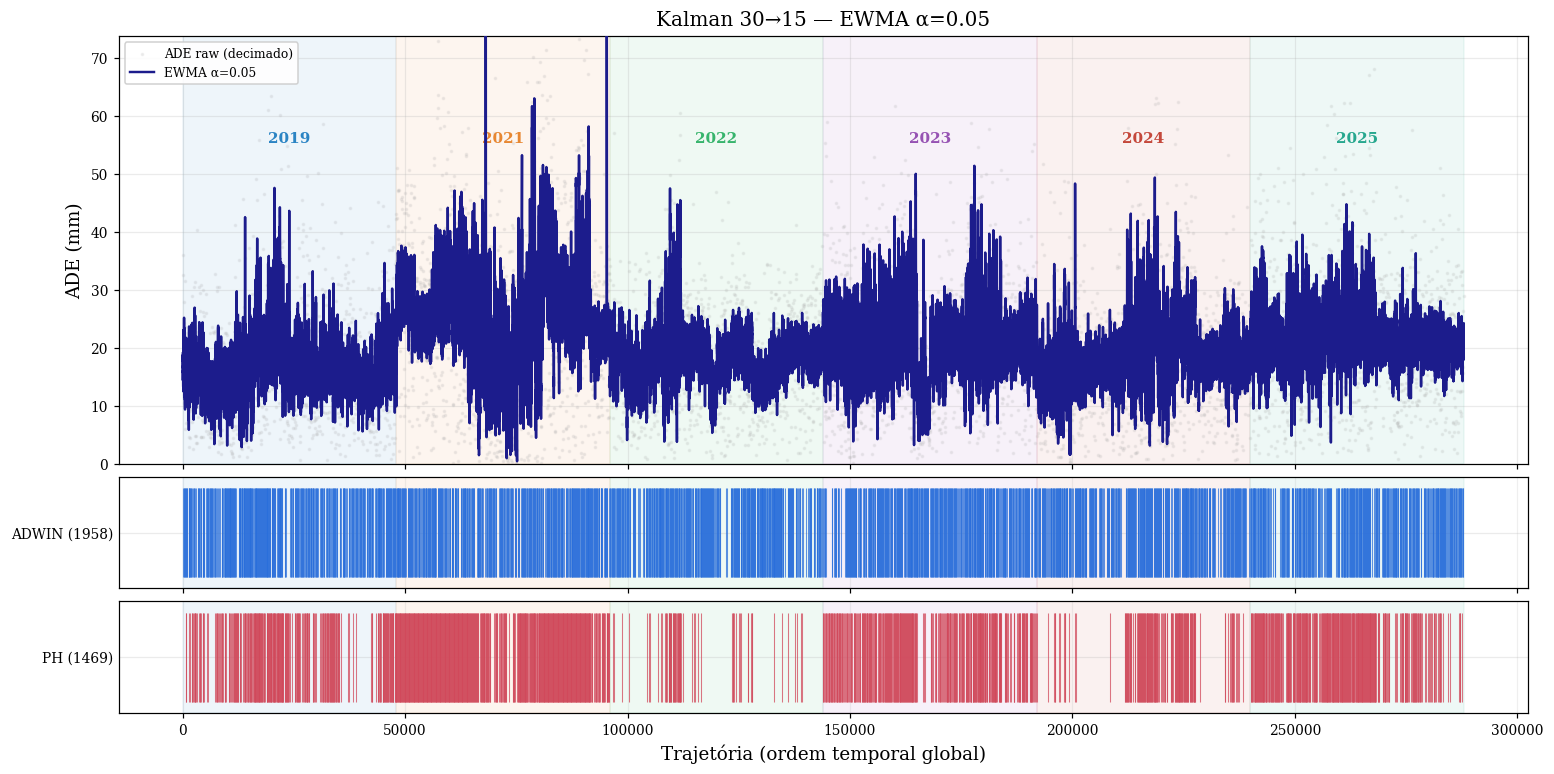
\includegraphics[width=\linewidth]{../mes9_phase1/images/ewma_a005/ewma_a005_kalman}\caption{\texttt{ewma\_a005} --- Kalman.}\end{subfigure}

\vspace{0.3em}
\begin{subfigure}[b]{0.48\textwidth}\centering
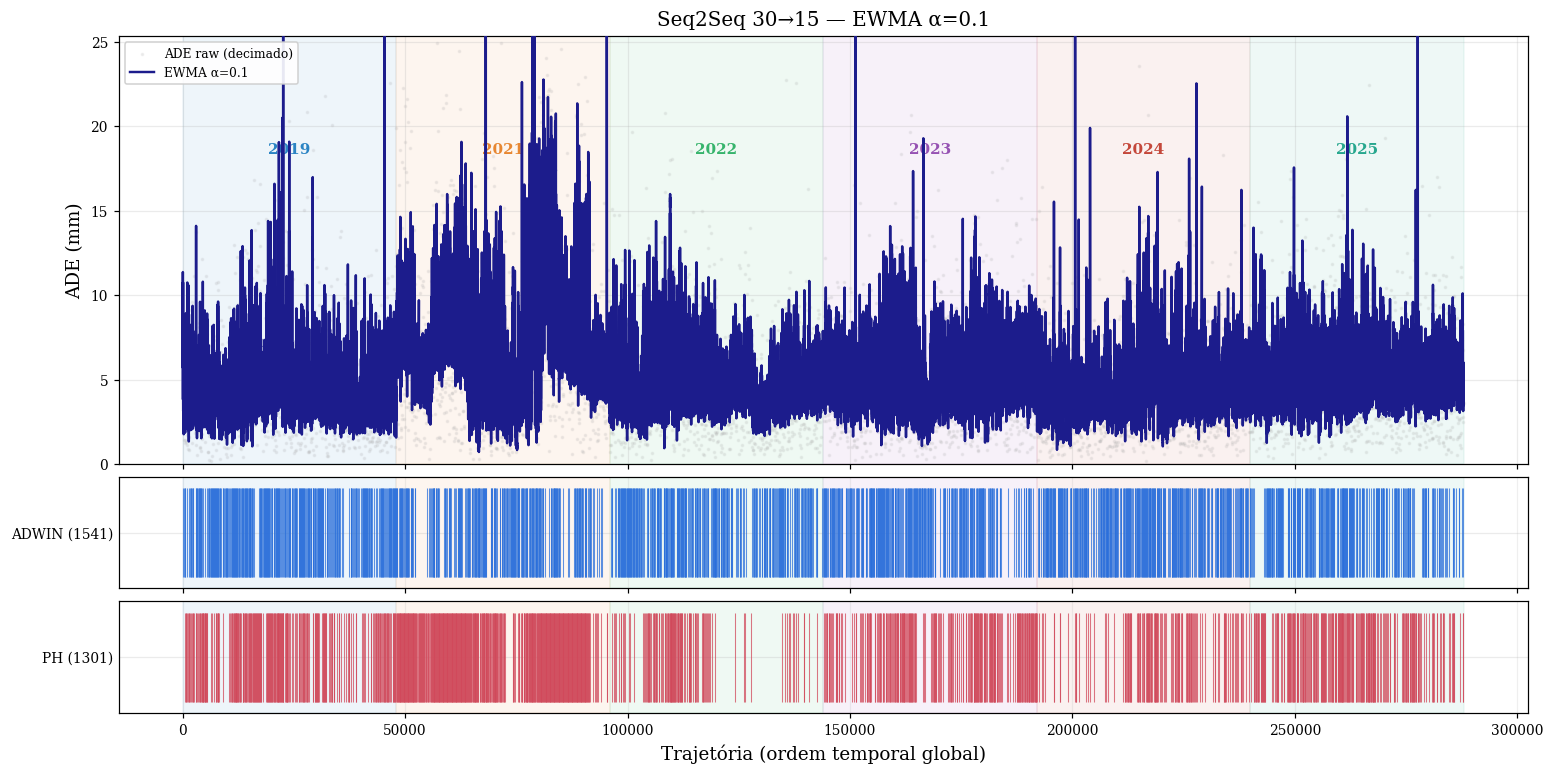
\includegraphics[width=\linewidth]{../mes9_phase1/images/ewma_a010/ewma_a010_seq2seq}\caption{\texttt{ewma\_a010} --- S2S.}\end{subfigure}\hfill
\begin{subfigure}[b]{0.48\textwidth}\centering
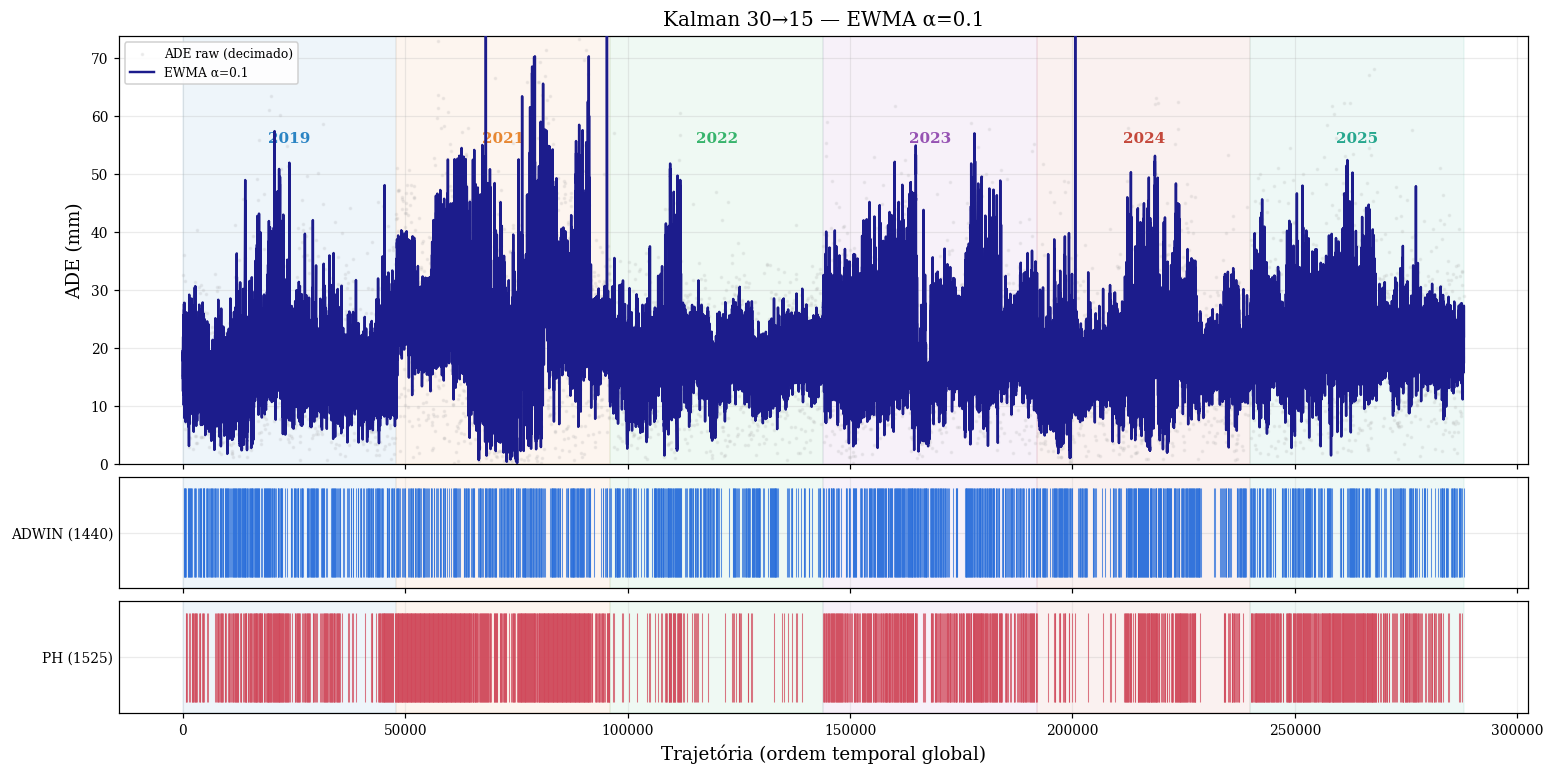
\includegraphics[width=\linewidth]{../mes9_phase1/images/ewma_a010/ewma_a010_kalman}\caption{\texttt{ewma\_a010} --- Kalman.}\end{subfigure}
\caption{\textbf{EWMA $\alpha$=0{,}05 e $\alpha$=0{,}10.}}
\label{fig:m9_p1_g7}
\end{figure}

\begin{figure}[H]
\centering
\begin{subfigure}[b]{0.48\textwidth}\centering
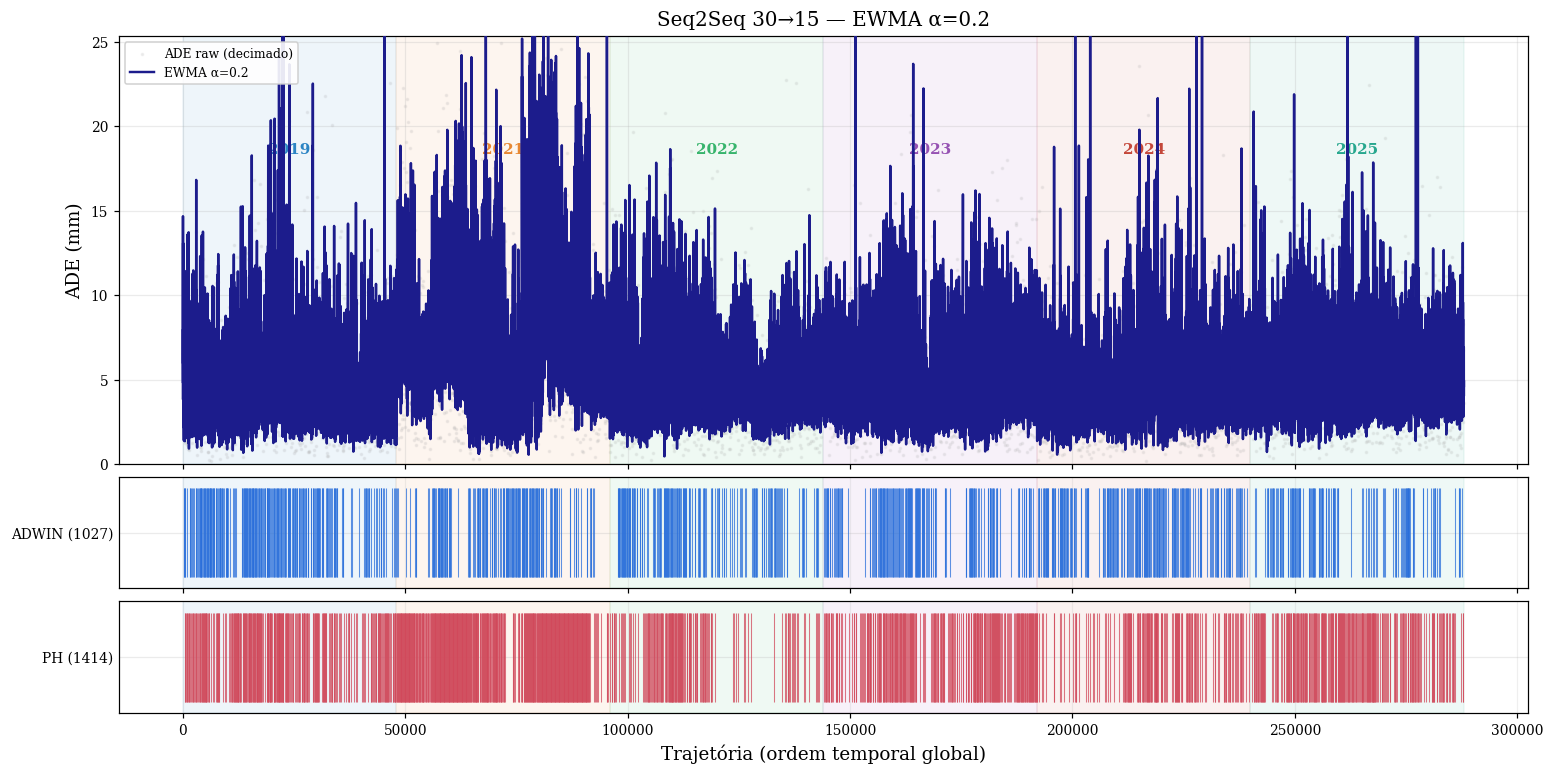
\includegraphics[width=\linewidth]{../mes9_phase1/images/ewma_a020/ewma_a020_seq2seq}\caption{\texttt{ewma\_a020} --- S2S.}\end{subfigure}\hfill
\begin{subfigure}[b]{0.48\textwidth}\centering
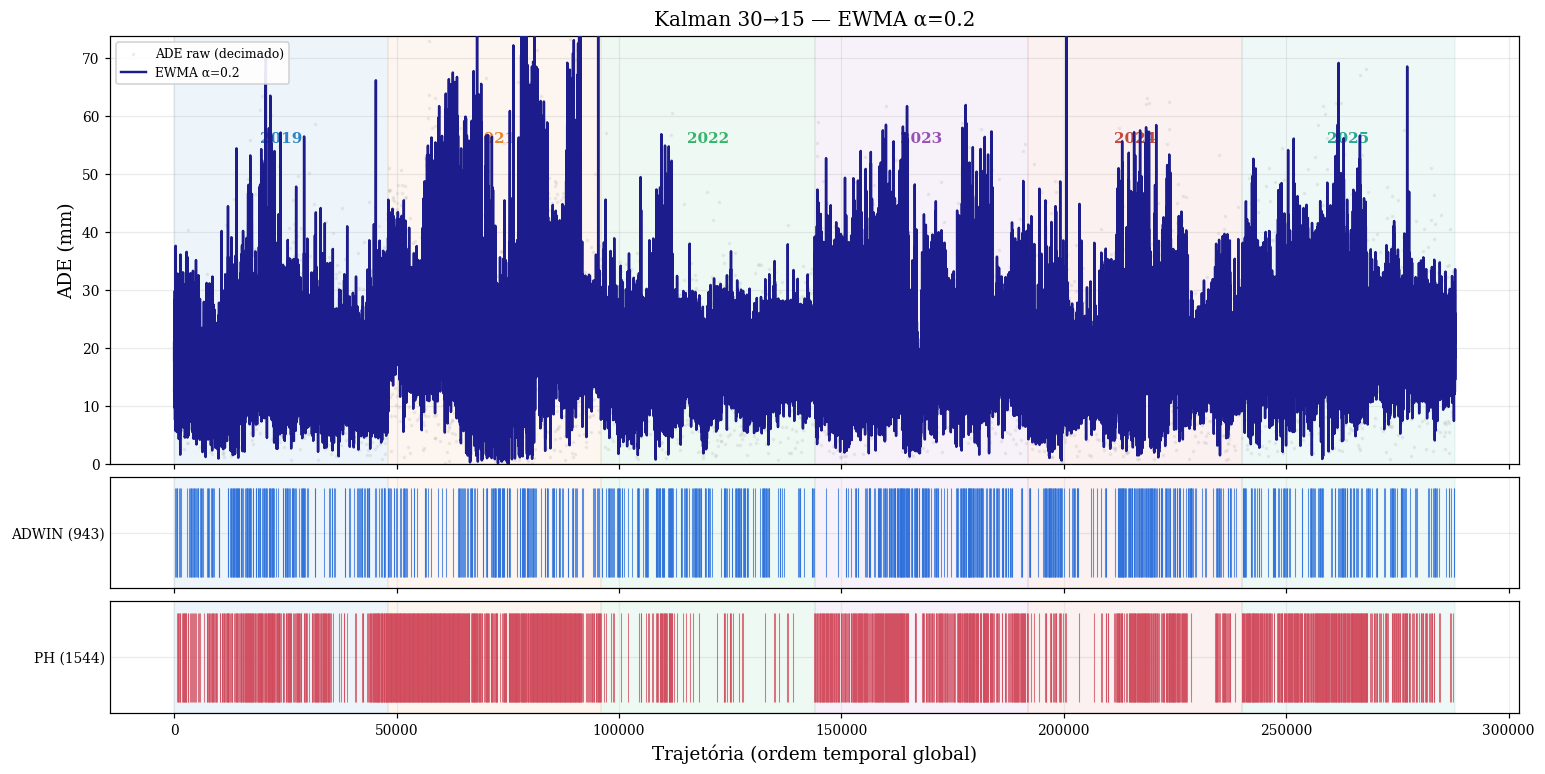
\includegraphics[width=\linewidth]{../mes9_phase1/images/ewma_a020/ewma_a020_kalman}\caption{\texttt{ewma\_a020} --- Kalman.}\end{subfigure}

\vspace{0.3em}
\begin{subfigure}[b]{0.48\textwidth}\centering
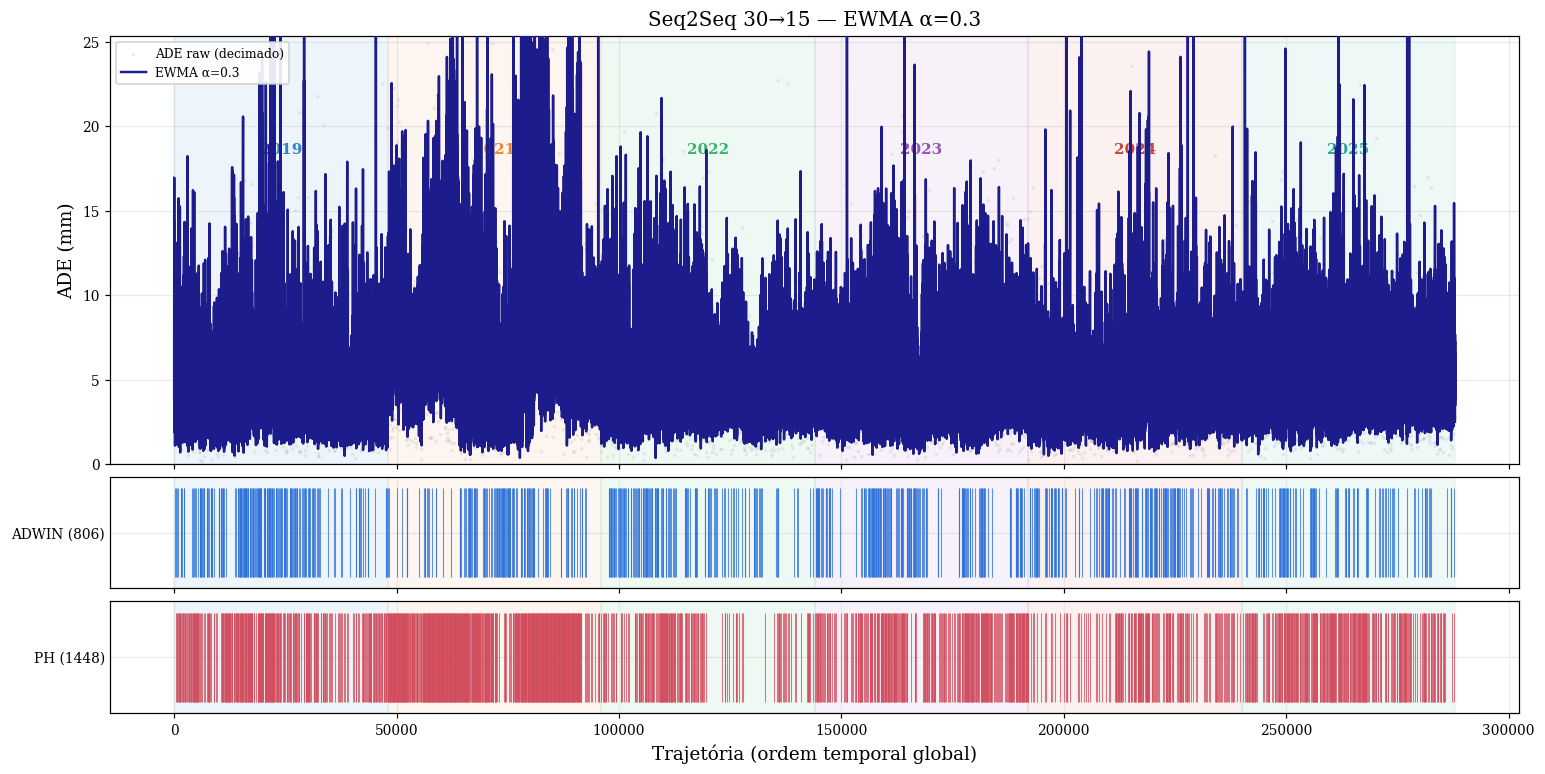
\includegraphics[width=\linewidth]{../mes9_phase1/images/ewma_a030/ewma_a030_seq2seq}\caption{\texttt{ewma\_a030} --- S2S.}\end{subfigure}\hfill
\begin{subfigure}[b]{0.48\textwidth}\centering
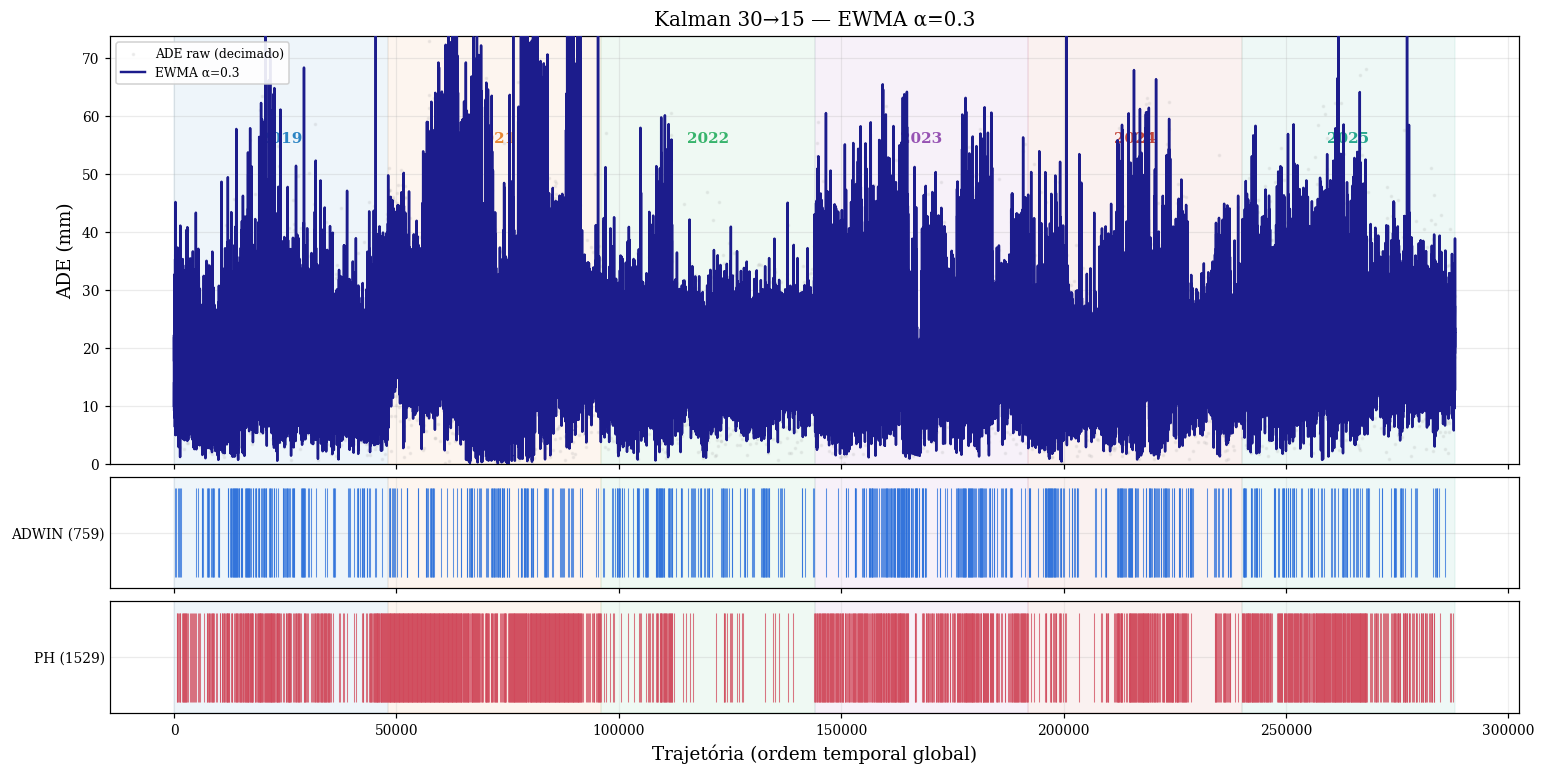
\includegraphics[width=\linewidth]{../mes9_phase1/images/ewma_a030/ewma_a030_kalman}\caption{\texttt{ewma\_a030} --- Kalman.}\end{subfigure}
\caption{\textbf{EWMA $\alpha$=0{,}20 e $\alpha$=0{,}30.}
         Mesmo com $\alpha$ alto (resposta r\'apida), o EWMA aumenta a
         FAR\textsubscript{2019} para 3--5/1k no Seq2Seq.}
\label{fig:m9_p1_g8}
\end{figure}

\begin{figure}[H]
\centering
\begin{subfigure}[b]{0.48\textwidth}\centering
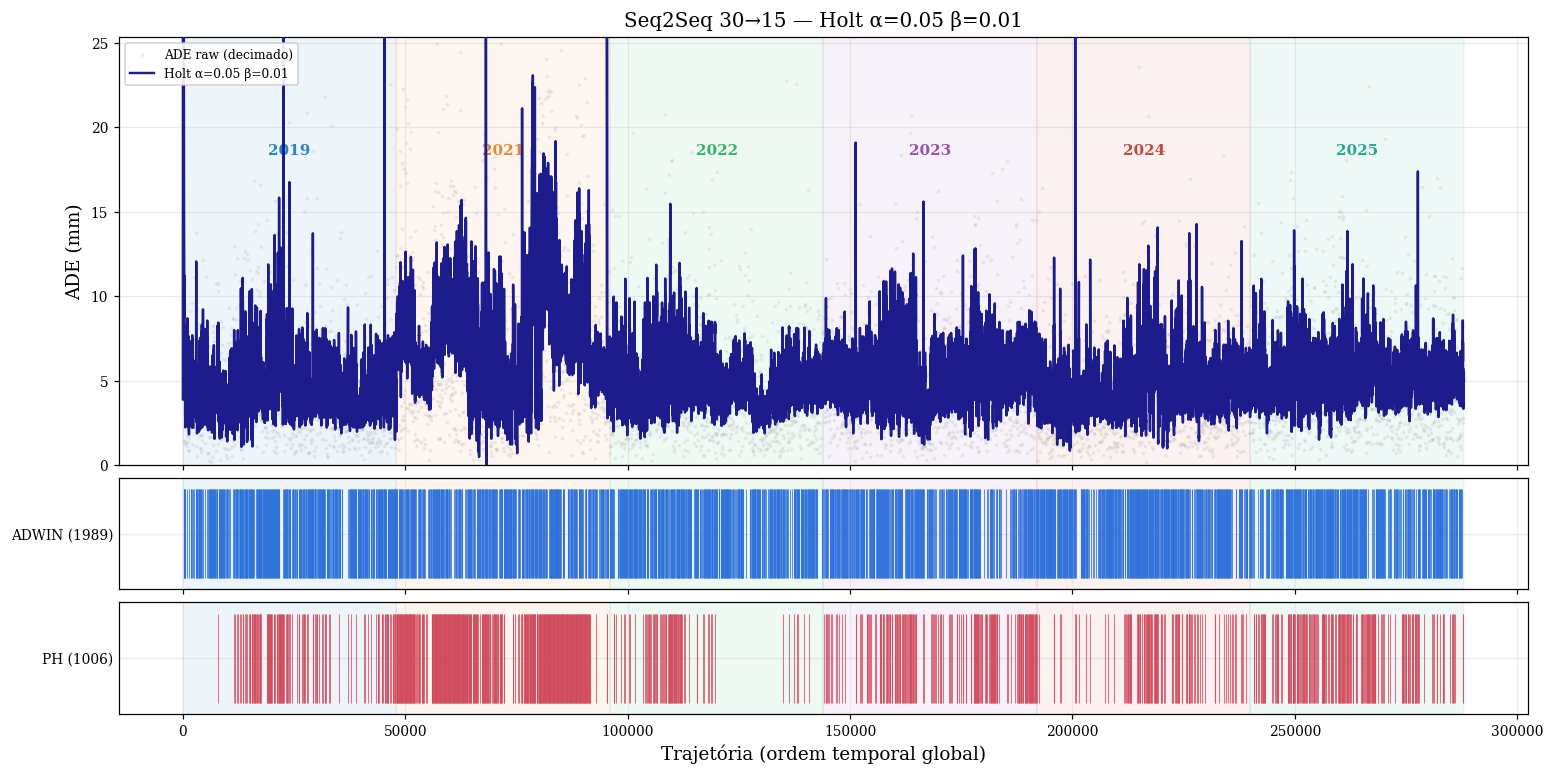
\includegraphics[width=\linewidth]{../mes9_phase1/images/holt_a005_b001/holt_a005_b001_seq2seq}\caption{\texttt{holt\_a005\_b001} --- S2S.}\end{subfigure}\hfill
\begin{subfigure}[b]{0.48\textwidth}\centering
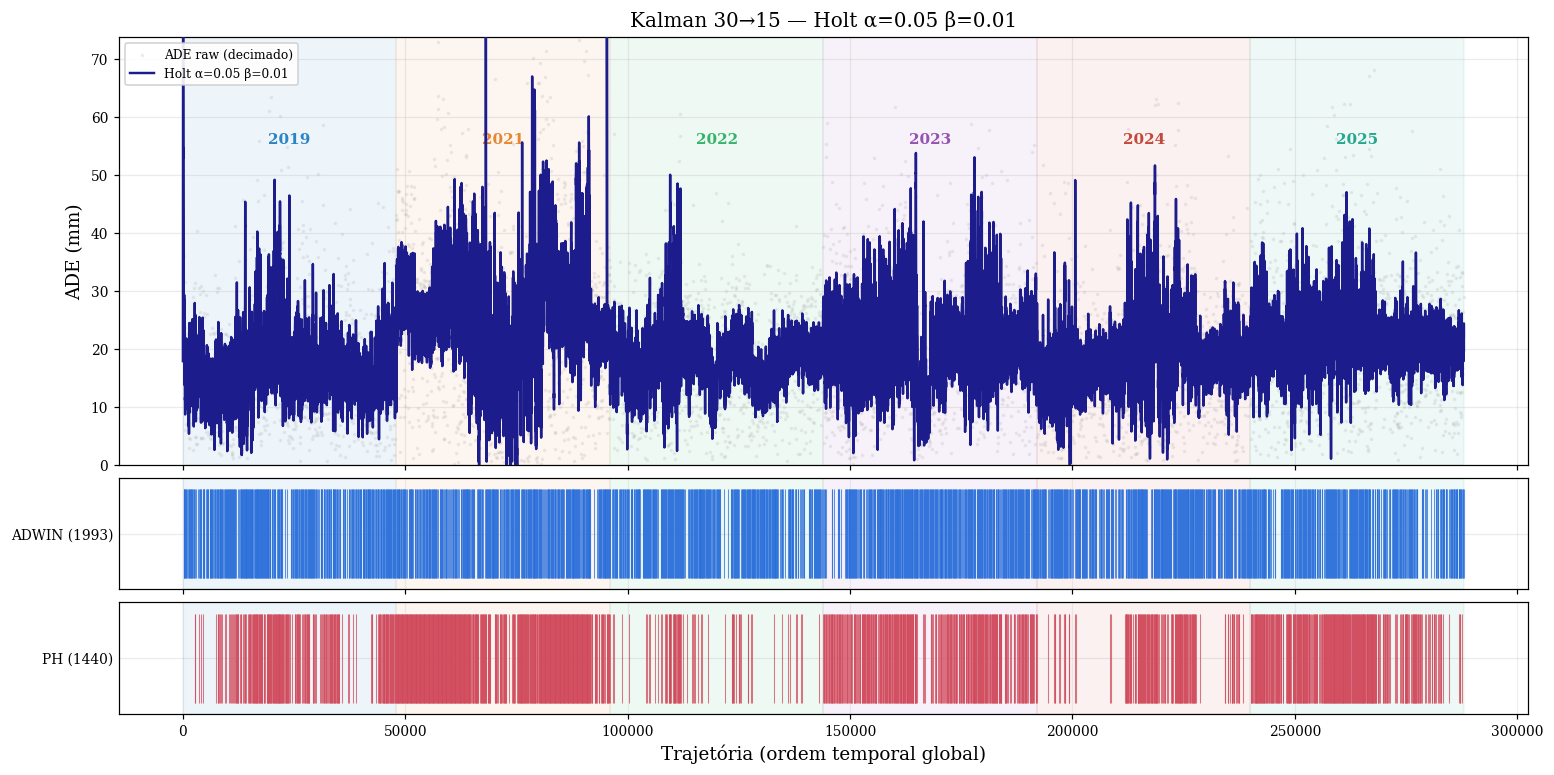
\includegraphics[width=\linewidth]{../mes9_phase1/images/holt_a005_b001/holt_a005_b001_kalman}\caption{\texttt{holt\_a005\_b001} --- Kalman.}\end{subfigure}

\vspace{0.3em}
\begin{subfigure}[b]{0.48\textwidth}\centering
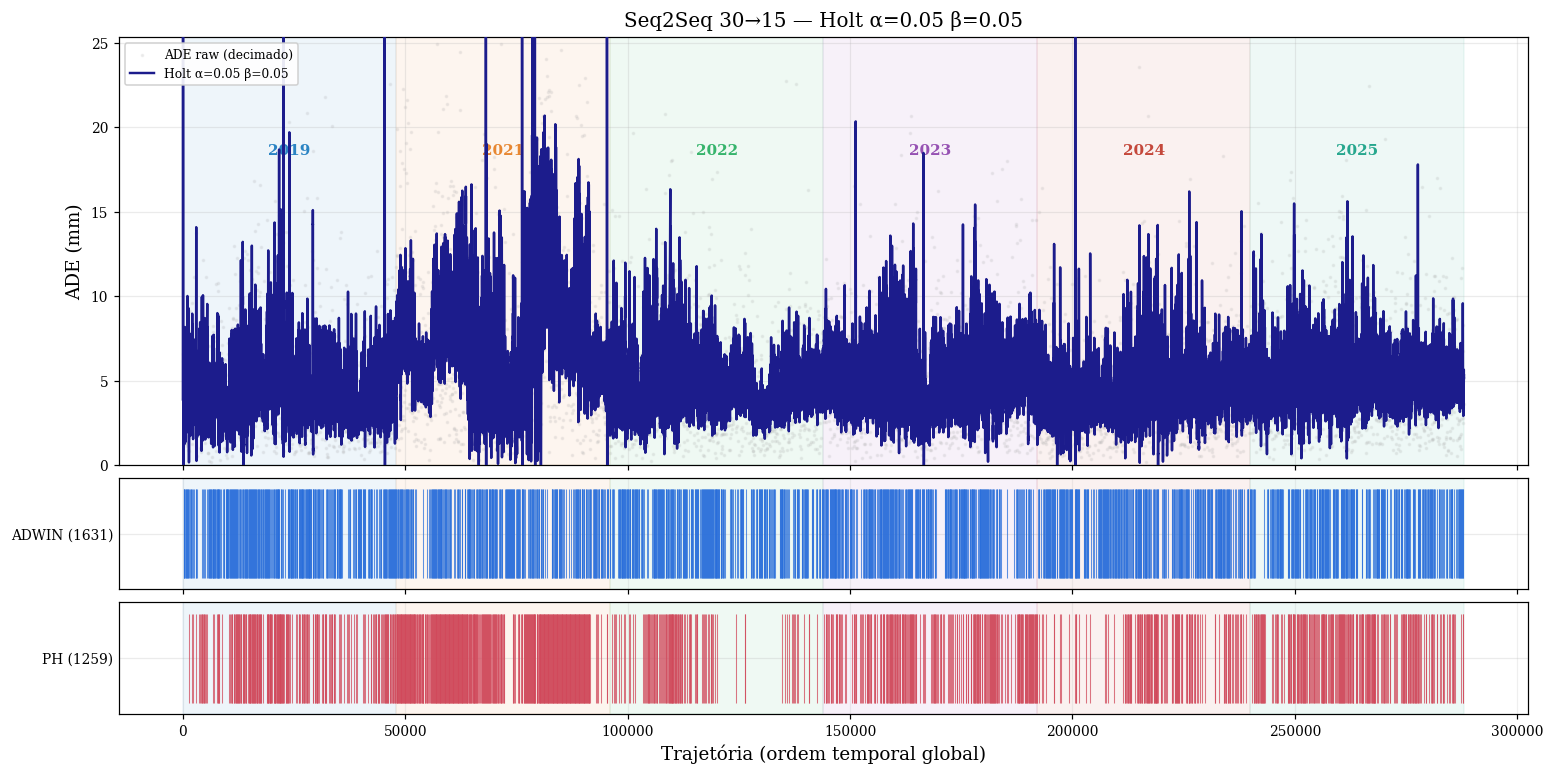
\includegraphics[width=\linewidth]{../mes9_phase1/images/holt_a005_b005/holt_a005_b005_seq2seq}\caption{\texttt{holt\_a005\_b005} --- S2S.}\end{subfigure}\hfill
\begin{subfigure}[b]{0.48\textwidth}\centering
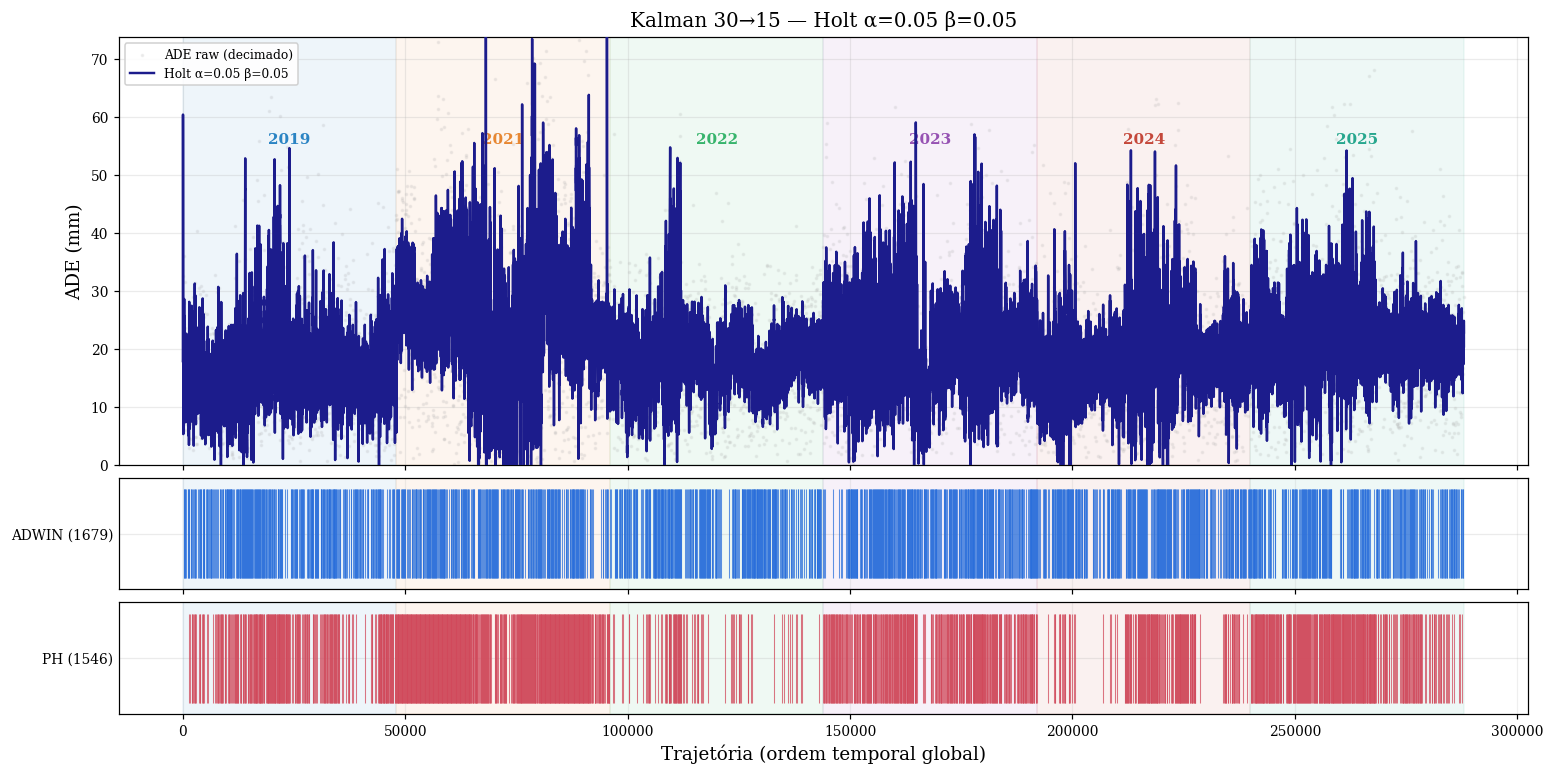
\includegraphics[width=\linewidth]{../mes9_phase1/images/holt_a005_b005/holt_a005_b005_kalman}\caption{\texttt{holt\_a005\_b005} --- Kalman.}\end{subfigure}
\caption{\textbf{Holt $\alpha$=0{,}05, $\beta\!\in\!\{0{,}01;0{,}05\}$.}}
\label{fig:m9_p1_g9}
\end{figure}

\begin{figure}[H]
\centering
\begin{subfigure}[b]{0.48\textwidth}\centering
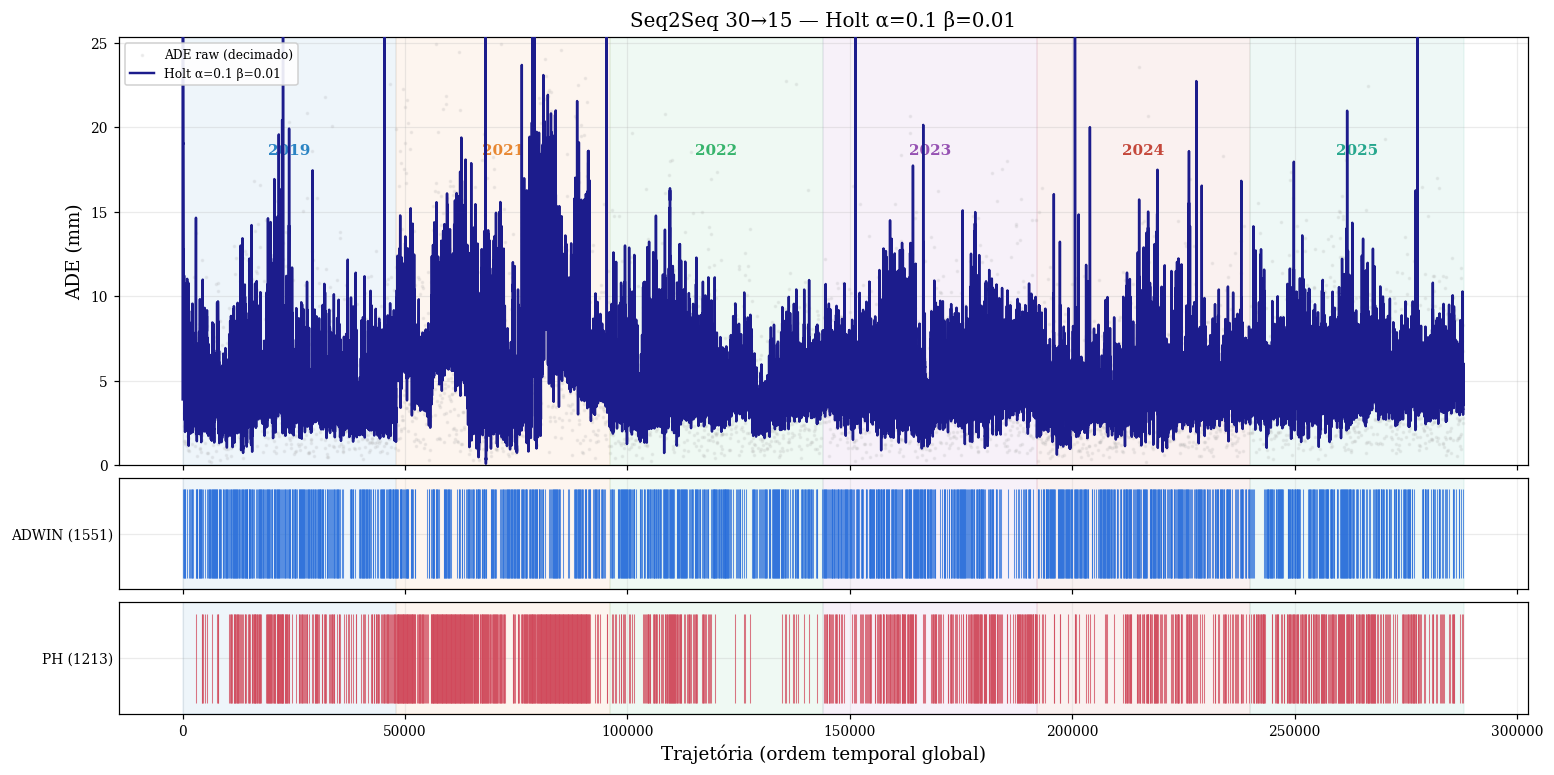
\includegraphics[width=\linewidth]{../mes9_phase1/images/holt_a010_b001/holt_a010_b001_seq2seq}\caption{\texttt{holt\_a010\_b001} --- S2S.}\end{subfigure}\hfill
\begin{subfigure}[b]{0.48\textwidth}\centering
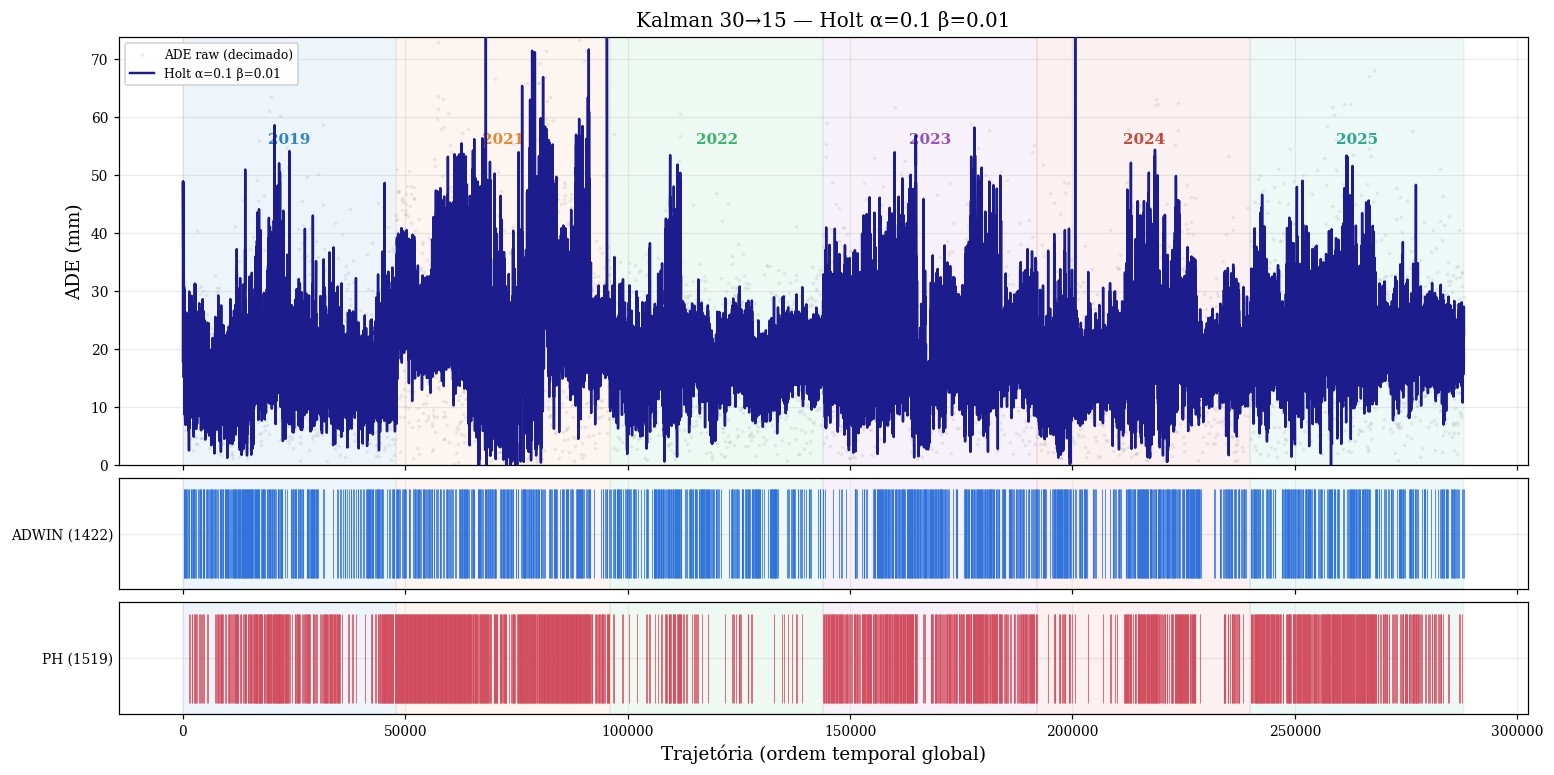
\includegraphics[width=\linewidth]{../mes9_phase1/images/holt_a010_b001/holt_a010_b001_kalman}\caption{\texttt{holt\_a010\_b001} --- Kalman.}\end{subfigure}

\vspace{0.3em}
\begin{subfigure}[b]{0.48\textwidth}\centering
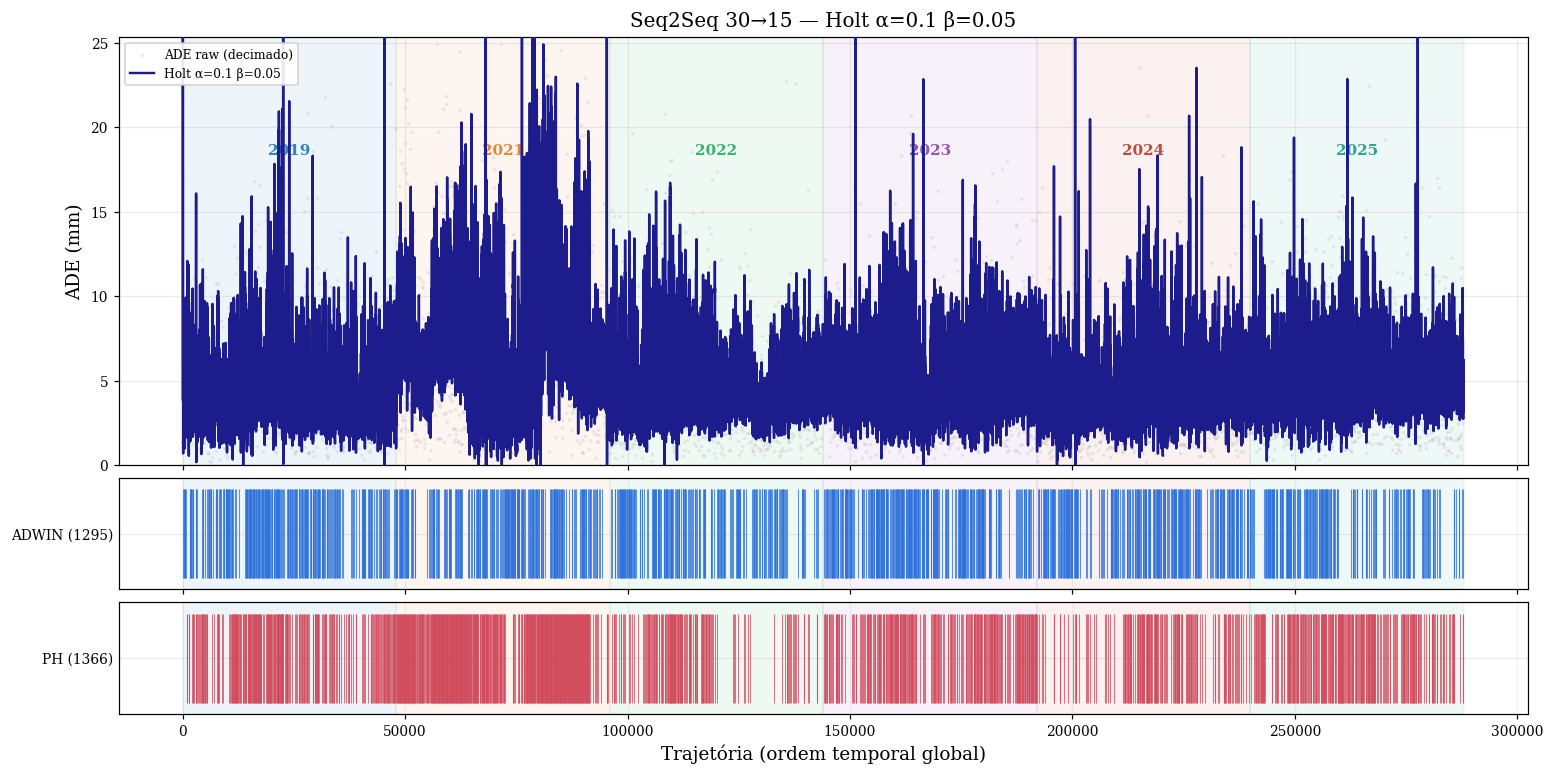
\includegraphics[width=\linewidth]{../mes9_phase1/images/holt_a010_b005/holt_a010_b005_seq2seq}\caption{\texttt{holt\_a010\_b005} --- S2S.}\end{subfigure}\hfill
\begin{subfigure}[b]{0.48\textwidth}\centering
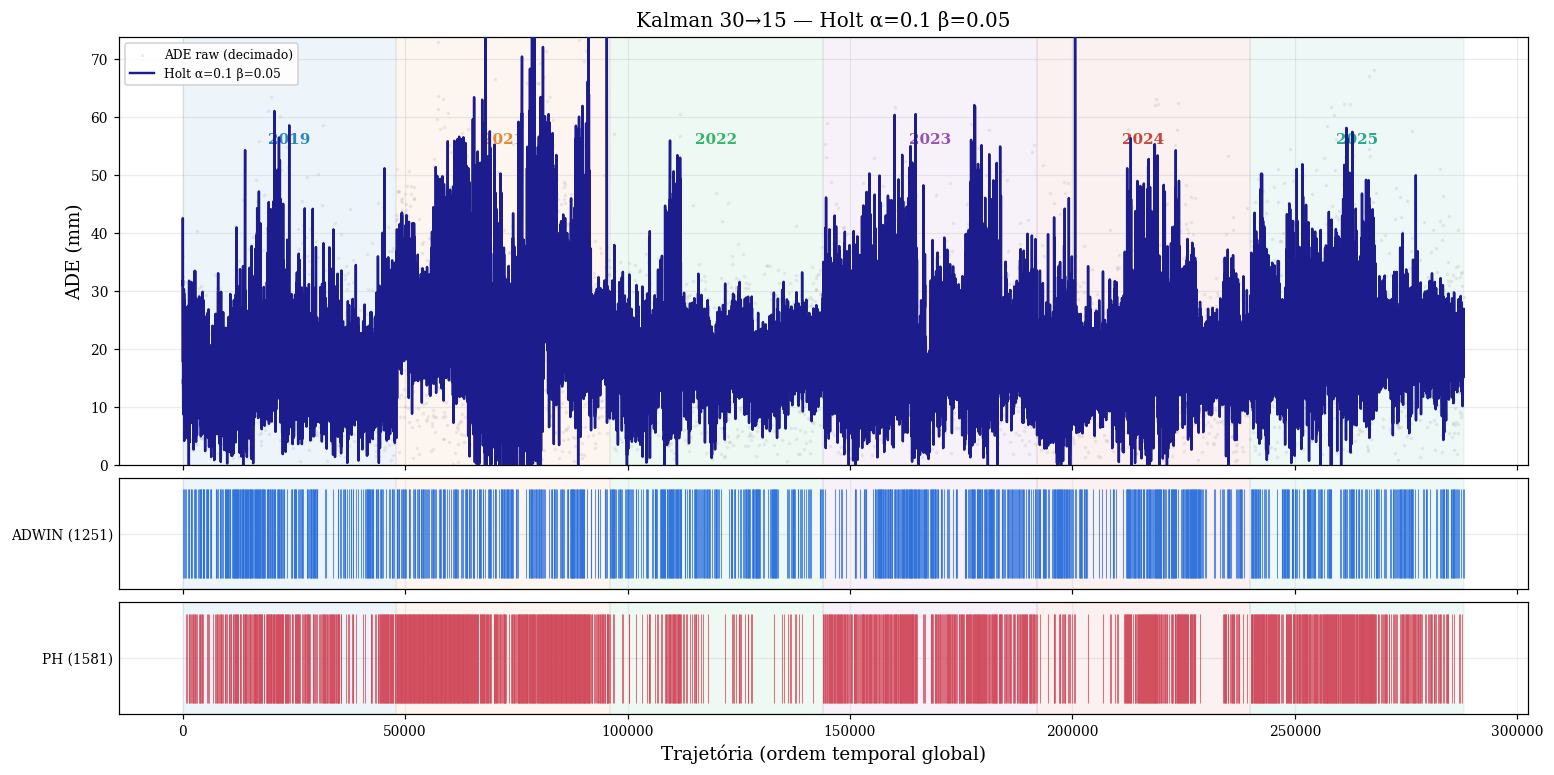
\includegraphics[width=\linewidth]{../mes9_phase1/images/holt_a010_b005/holt_a010_b005_kalman}\caption{\texttt{holt\_a010\_b005} --- Kalman.}\end{subfigure}
\caption{\textbf{Holt $\alpha$=0{,}10, $\beta\!\in\!\{0{,}01;0{,}05\}$.}}
\label{fig:m9_p1_g10}
\end{figure}

\begin{figure}[H]
\centering
\begin{subfigure}[b]{0.48\textwidth}\centering
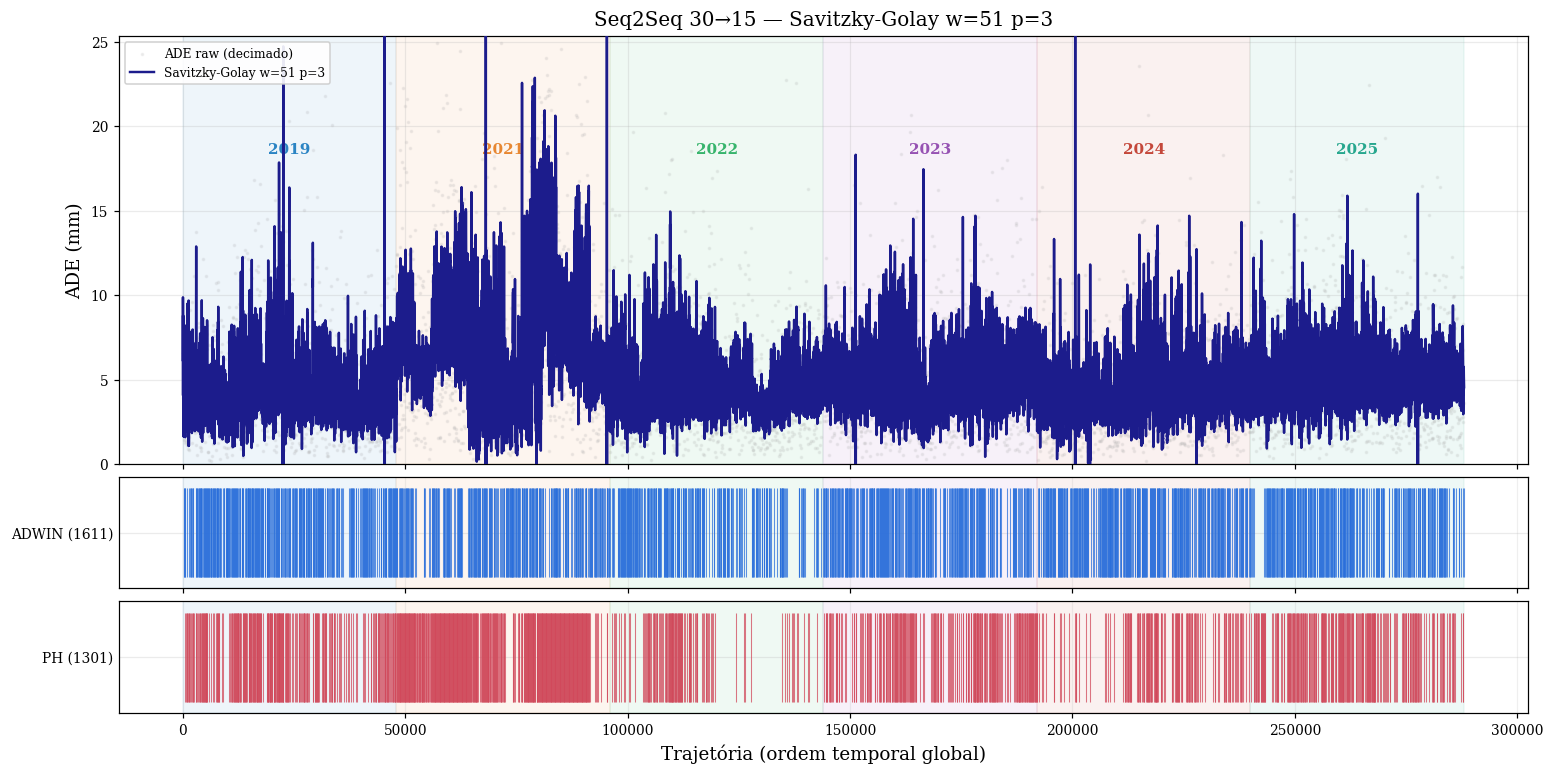
\includegraphics[width=\linewidth]{../mes9_phase1/images/savgol_w51_p3/savgol_w51_p3_seq2seq}\caption{\texttt{savgol\_w51\_p3} --- S2S.}\end{subfigure}\hfill
\begin{subfigure}[b]{0.48\textwidth}\centering
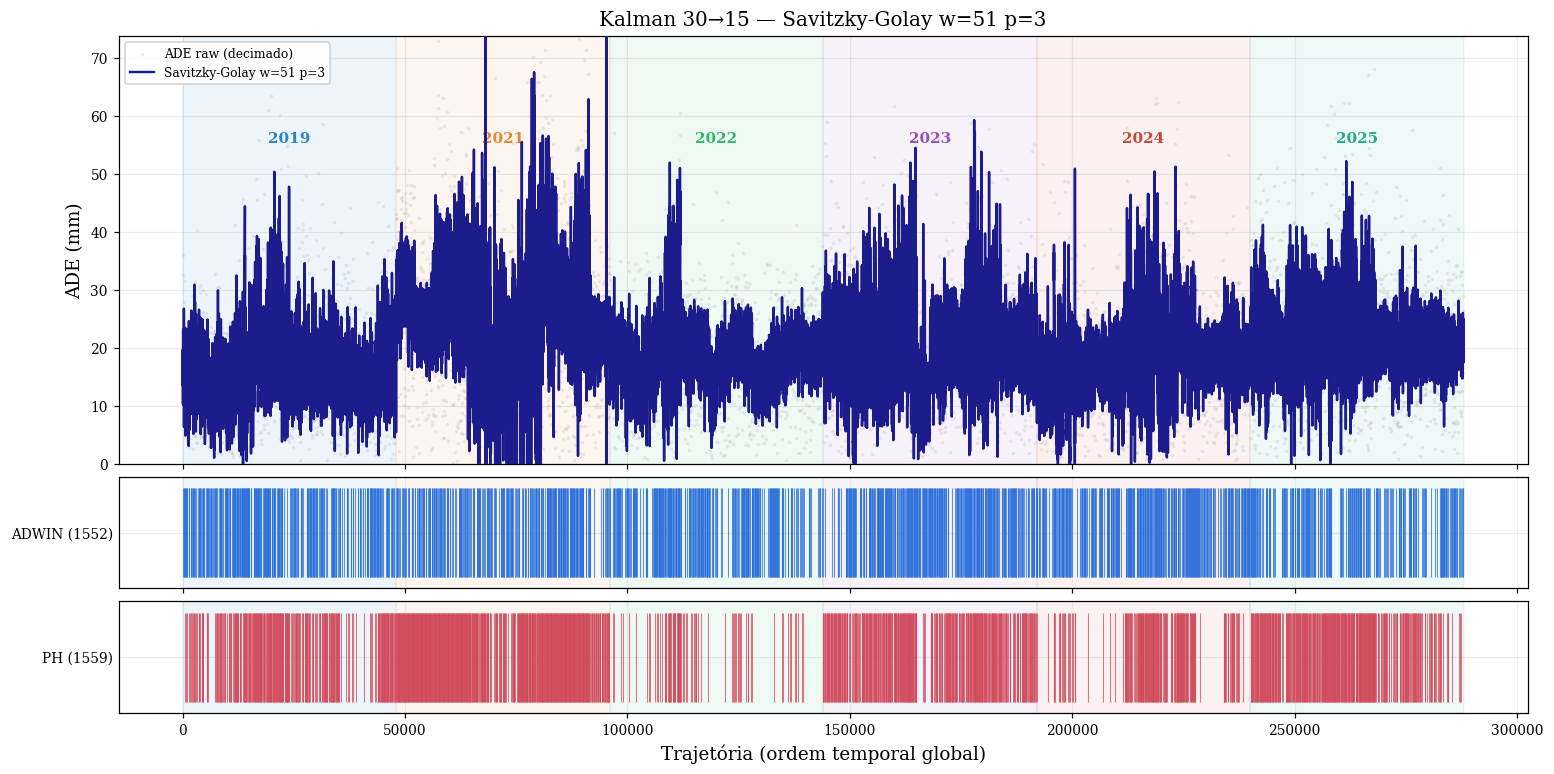
\includegraphics[width=\linewidth]{../mes9_phase1/images/savgol_w51_p3/savgol_w51_p3_kalman}\caption{\texttt{savgol\_w51\_p3} --- Kalman.}\end{subfigure}

\vspace{0.3em}
\begin{subfigure}[b]{0.48\textwidth}\centering
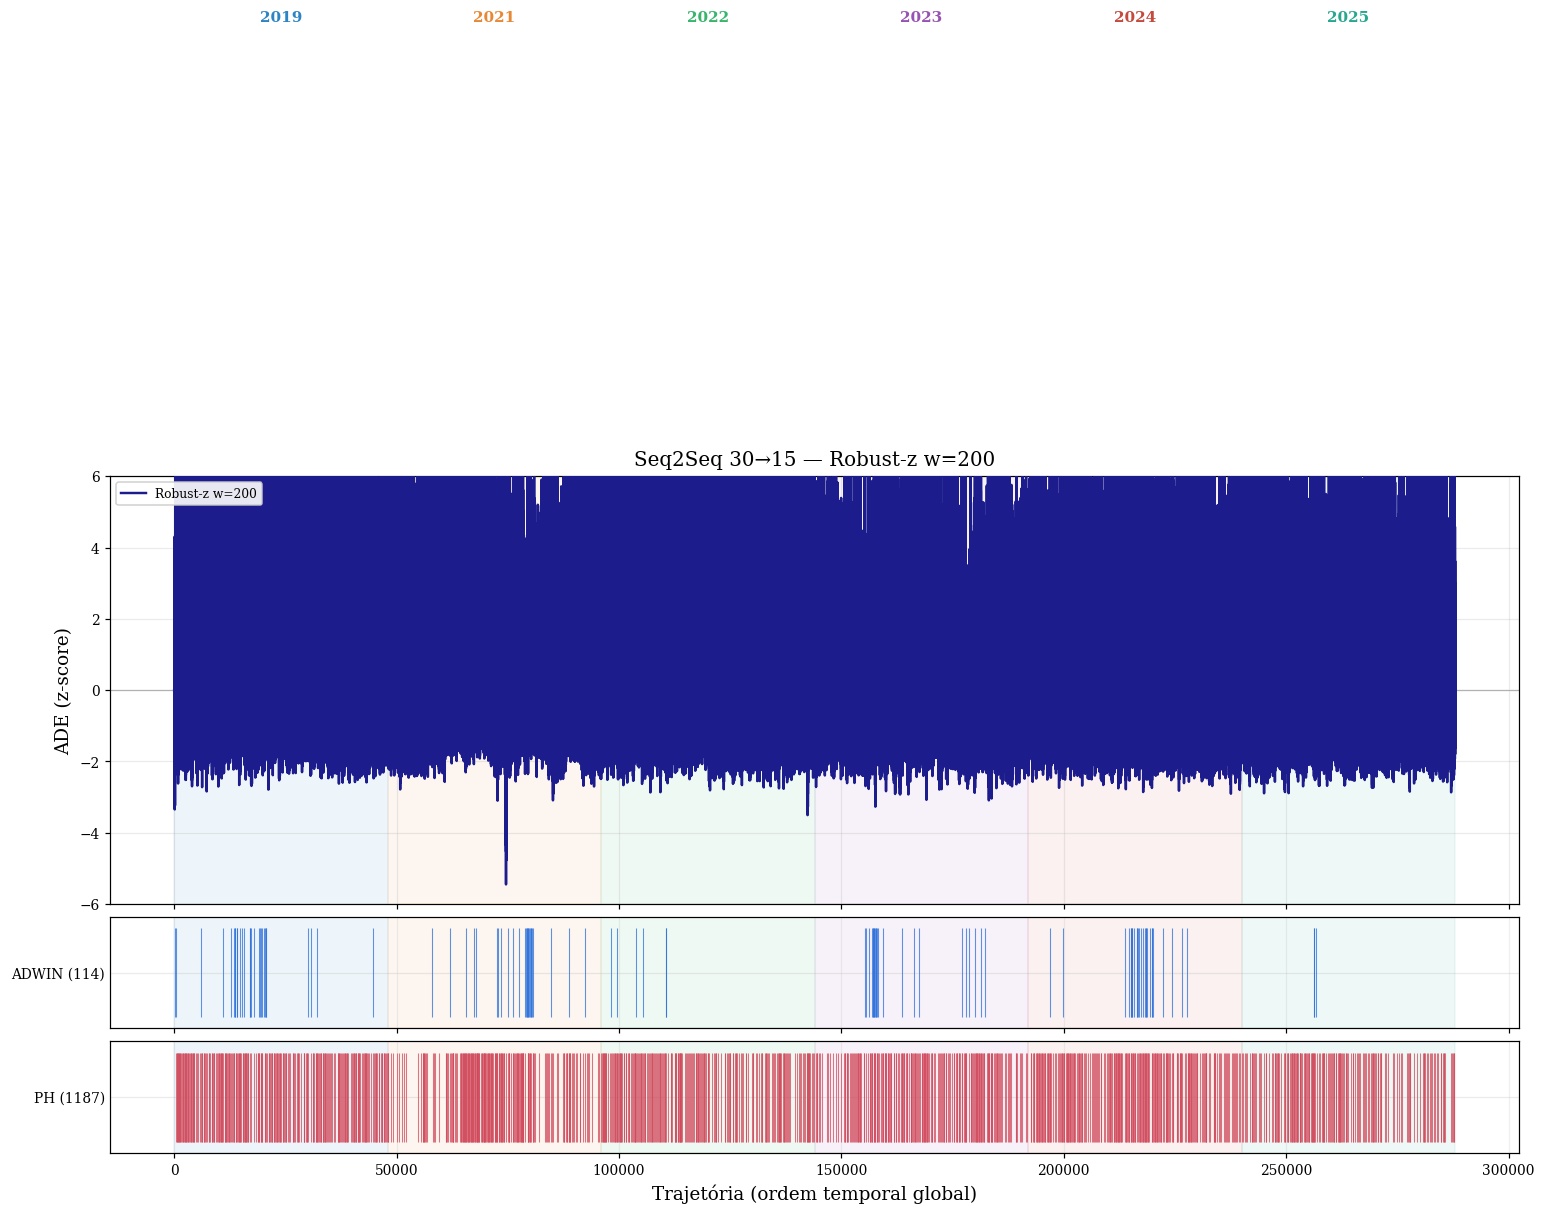
\includegraphics[width=\linewidth]{../mes9_phase1/images/robz_w200/robz_w200_seq2seq}\caption{\textbf{\texttt{robz\_w200}} --- S2S \textbf{(vencedor)}.}\end{subfigure}\hfill
\begin{subfigure}[b]{0.48\textwidth}\centering
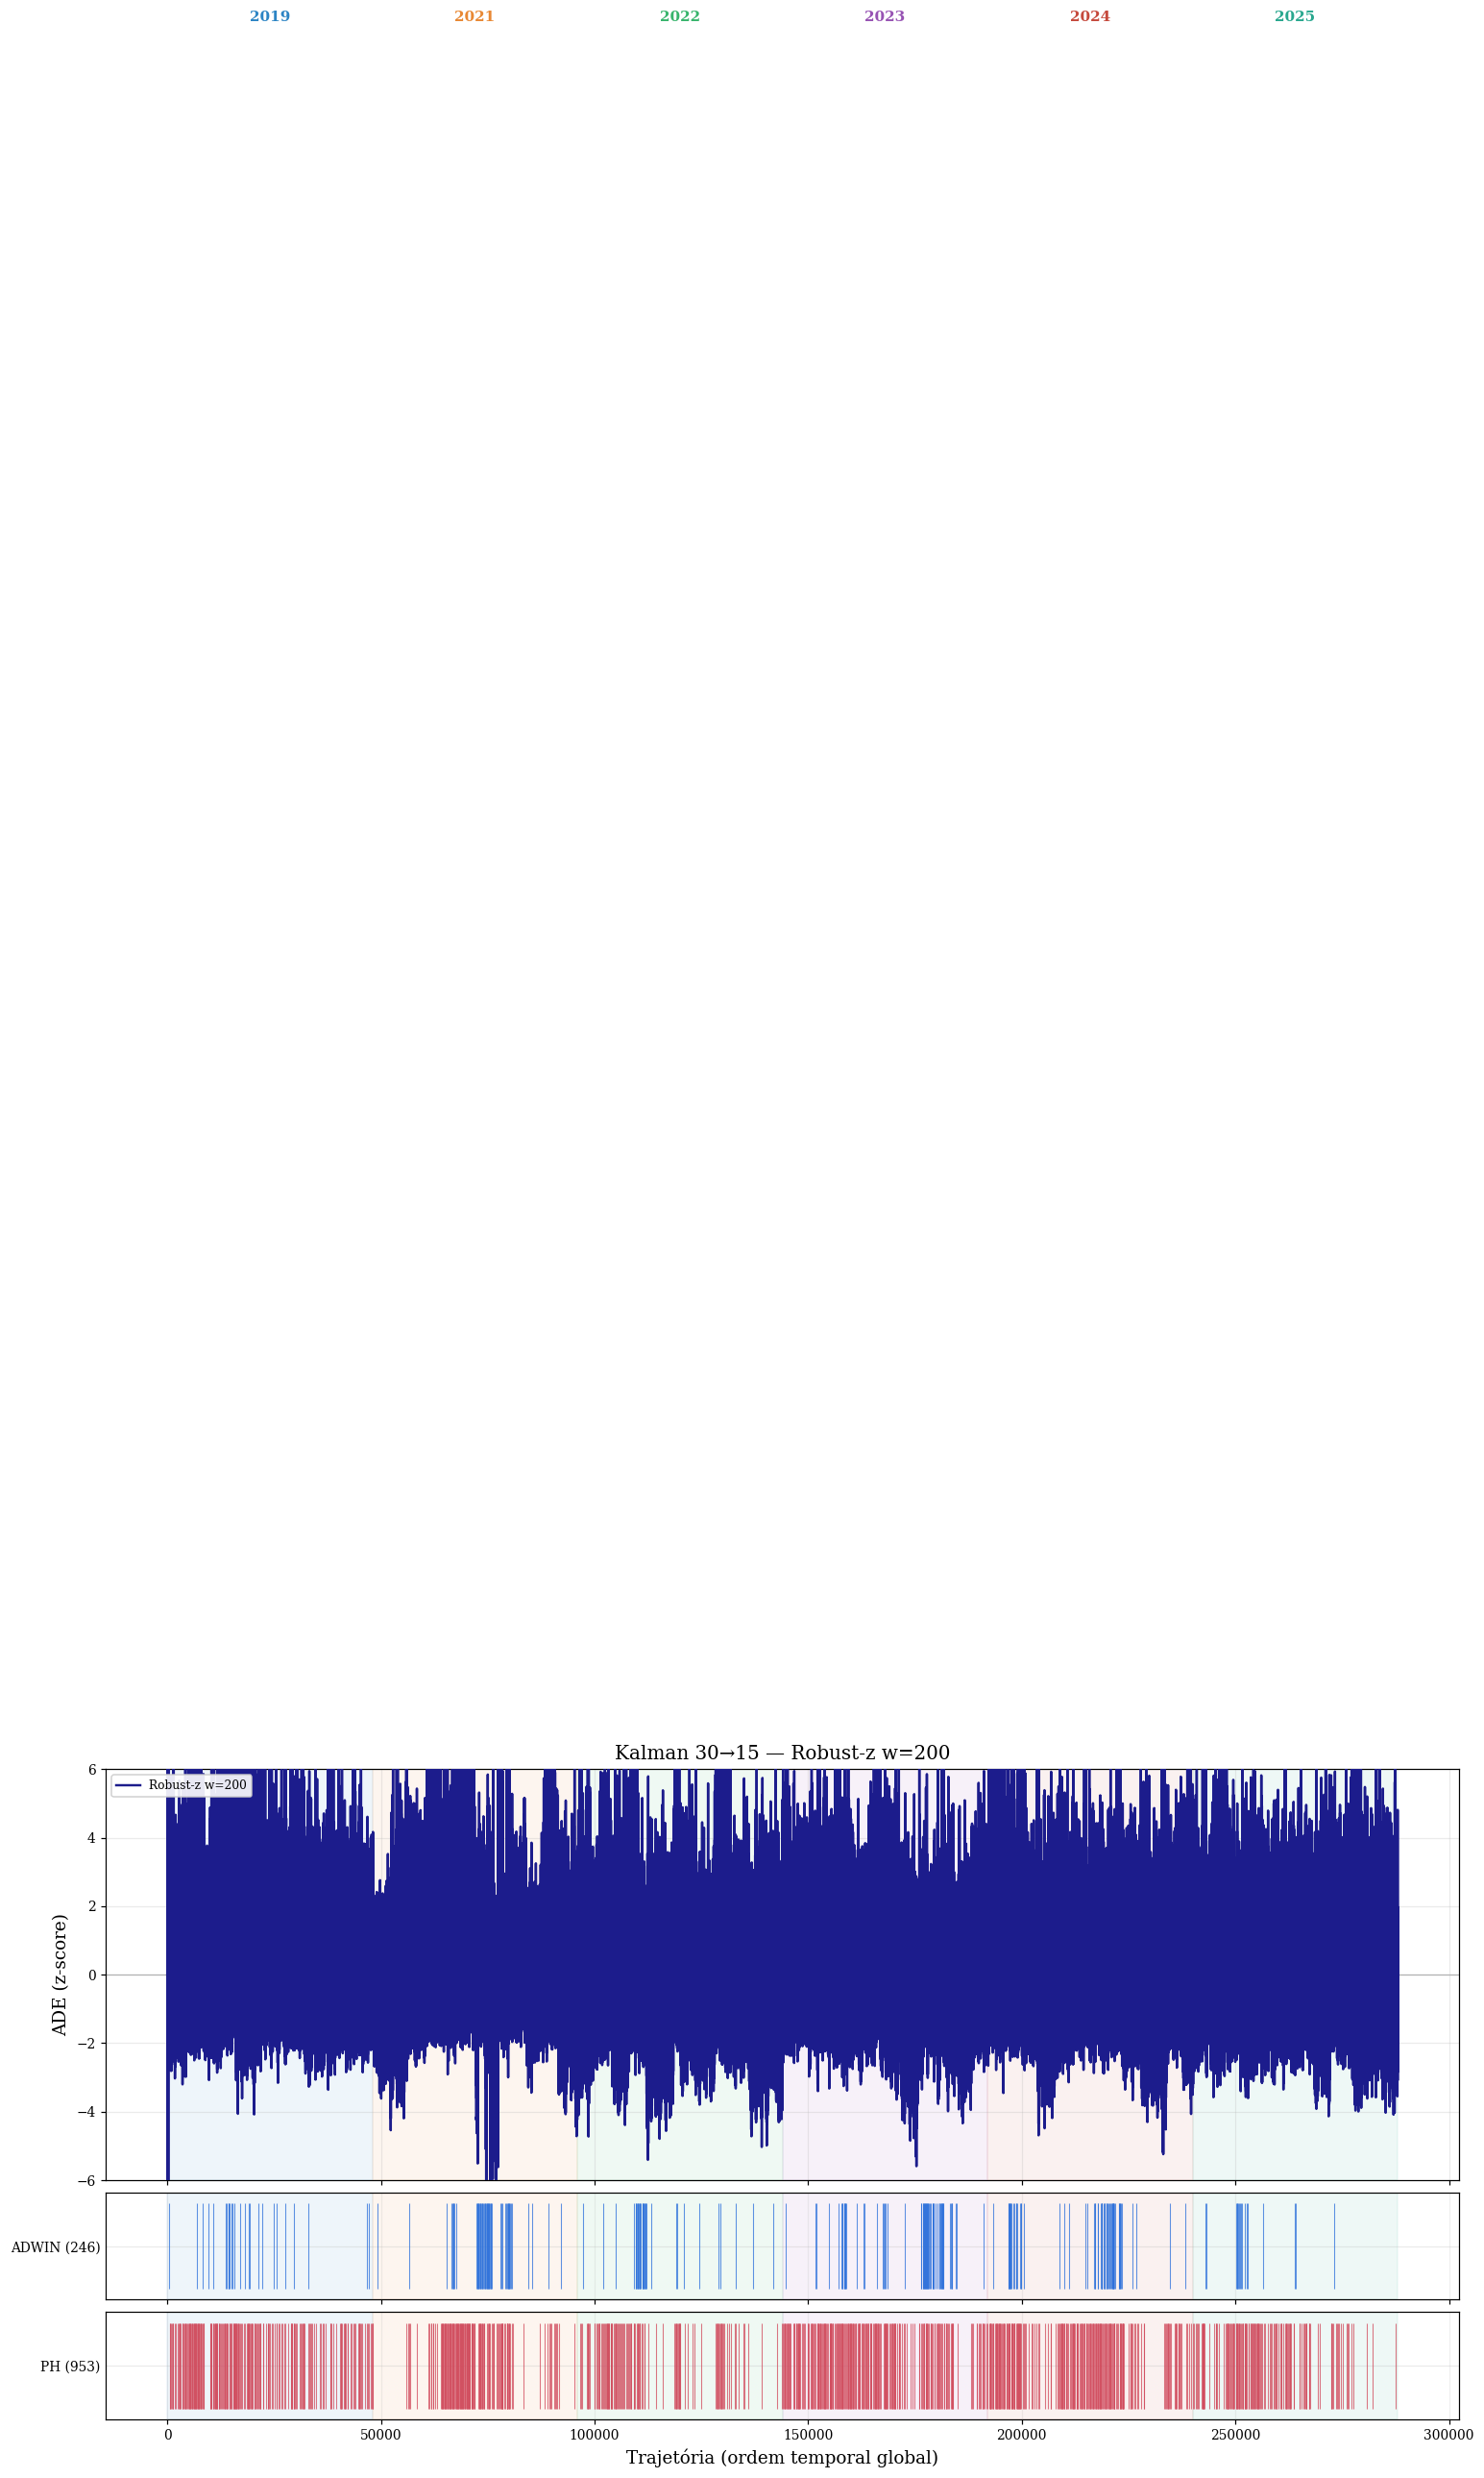
\includegraphics[width=\linewidth]{../mes9_phase1/images/robz_w200/robz_w200_kalman}\caption{\textbf{\texttt{robz\_w200}} --- Kalman \textbf{(vencedor)}.}\end{subfigure}
\caption{\textbf{Savitzky-Golay vs.\ Robust-z $w$=200 (o vencedor).}
         O \texttt{robz\_w200} \'e o \'unico pr\'e-processamento que
         \emph{reduz} a FAR\textsubscript{2019}: de 1{,}229/1k para
         0{,}604/1k no Seq2Seq (ADWIN), com var\_reduction\,$=$\,75{,}8\,\%
         e 85 alarmes p\'os-2019 (vs. 256 sem suaviza\c{c}\~ao). Esta
         \'e a base do grid search da Fase 2.}
\label{fig:m9_p1_g11}
\end{figure}

\begin{figure}[H]
\centering
\begin{subfigure}[b]{0.48\textwidth}\centering
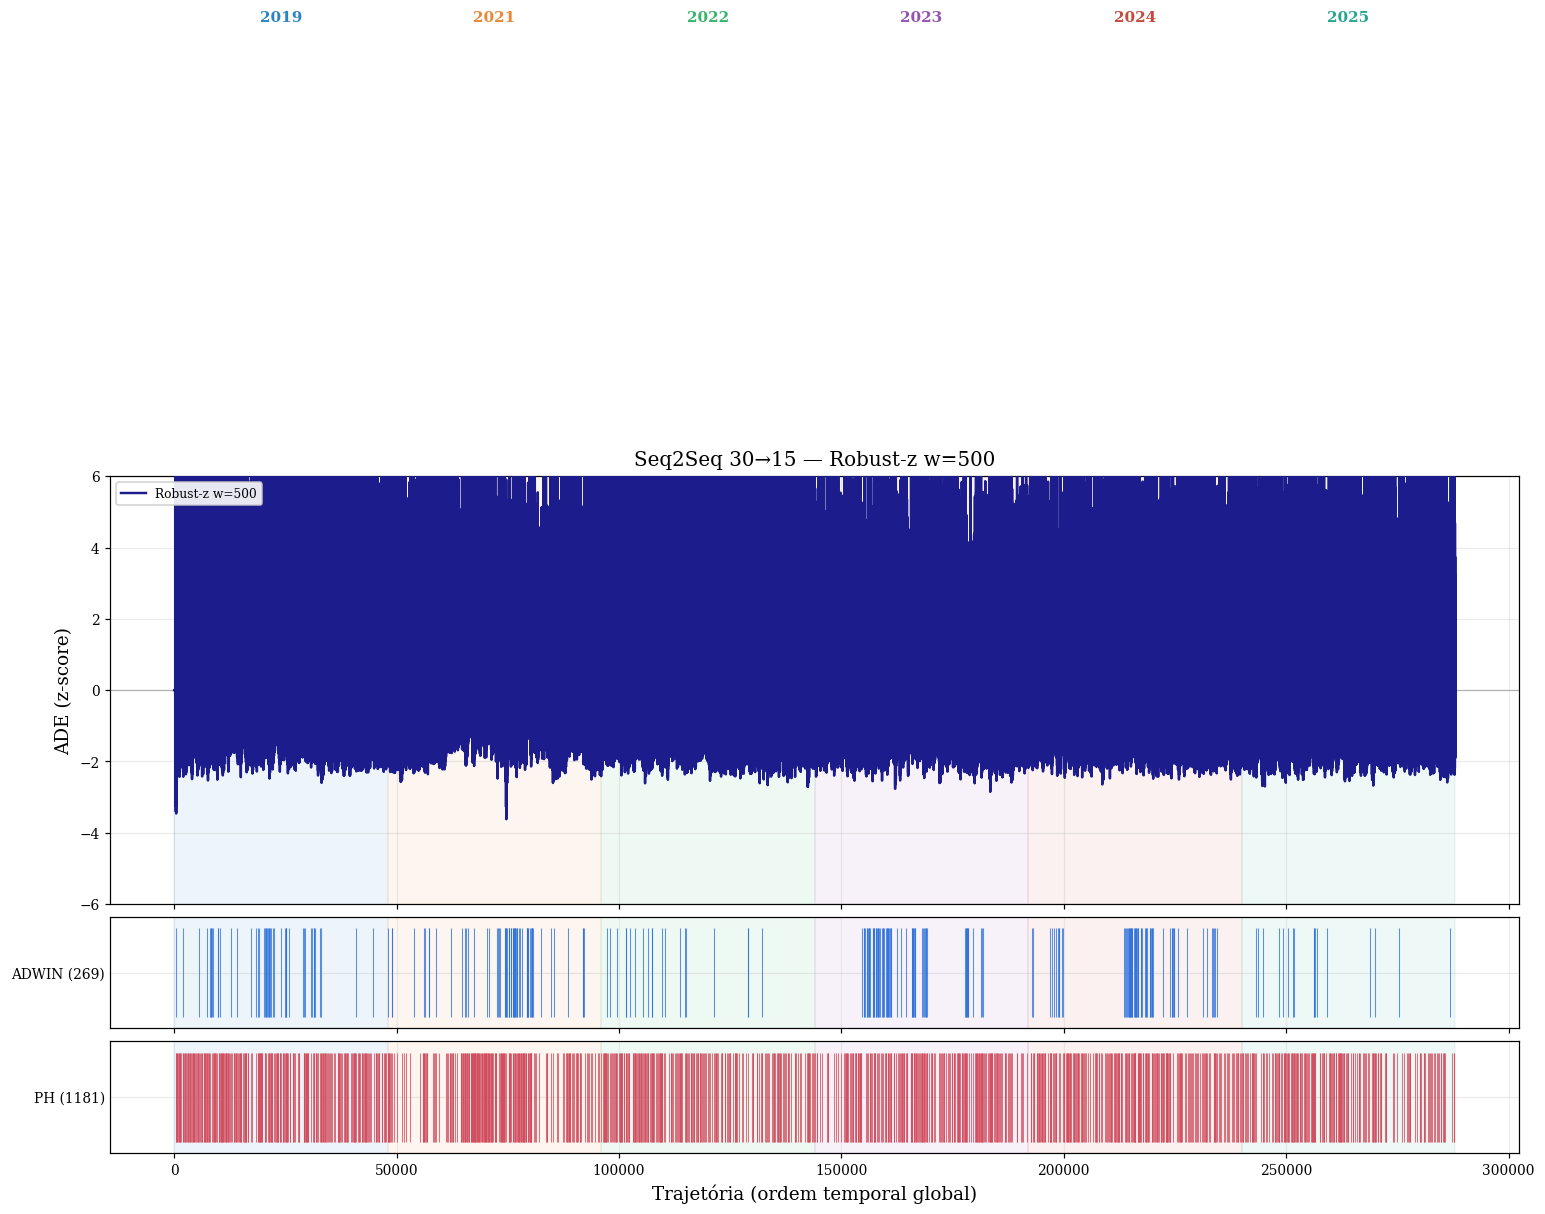
\includegraphics[width=\linewidth]{../mes9_phase1/images/robz_w500/robz_w500_seq2seq}\caption{\texttt{robz\_w500} --- S2S.}\end{subfigure}\hfill
\begin{subfigure}[b]{0.48\textwidth}\centering
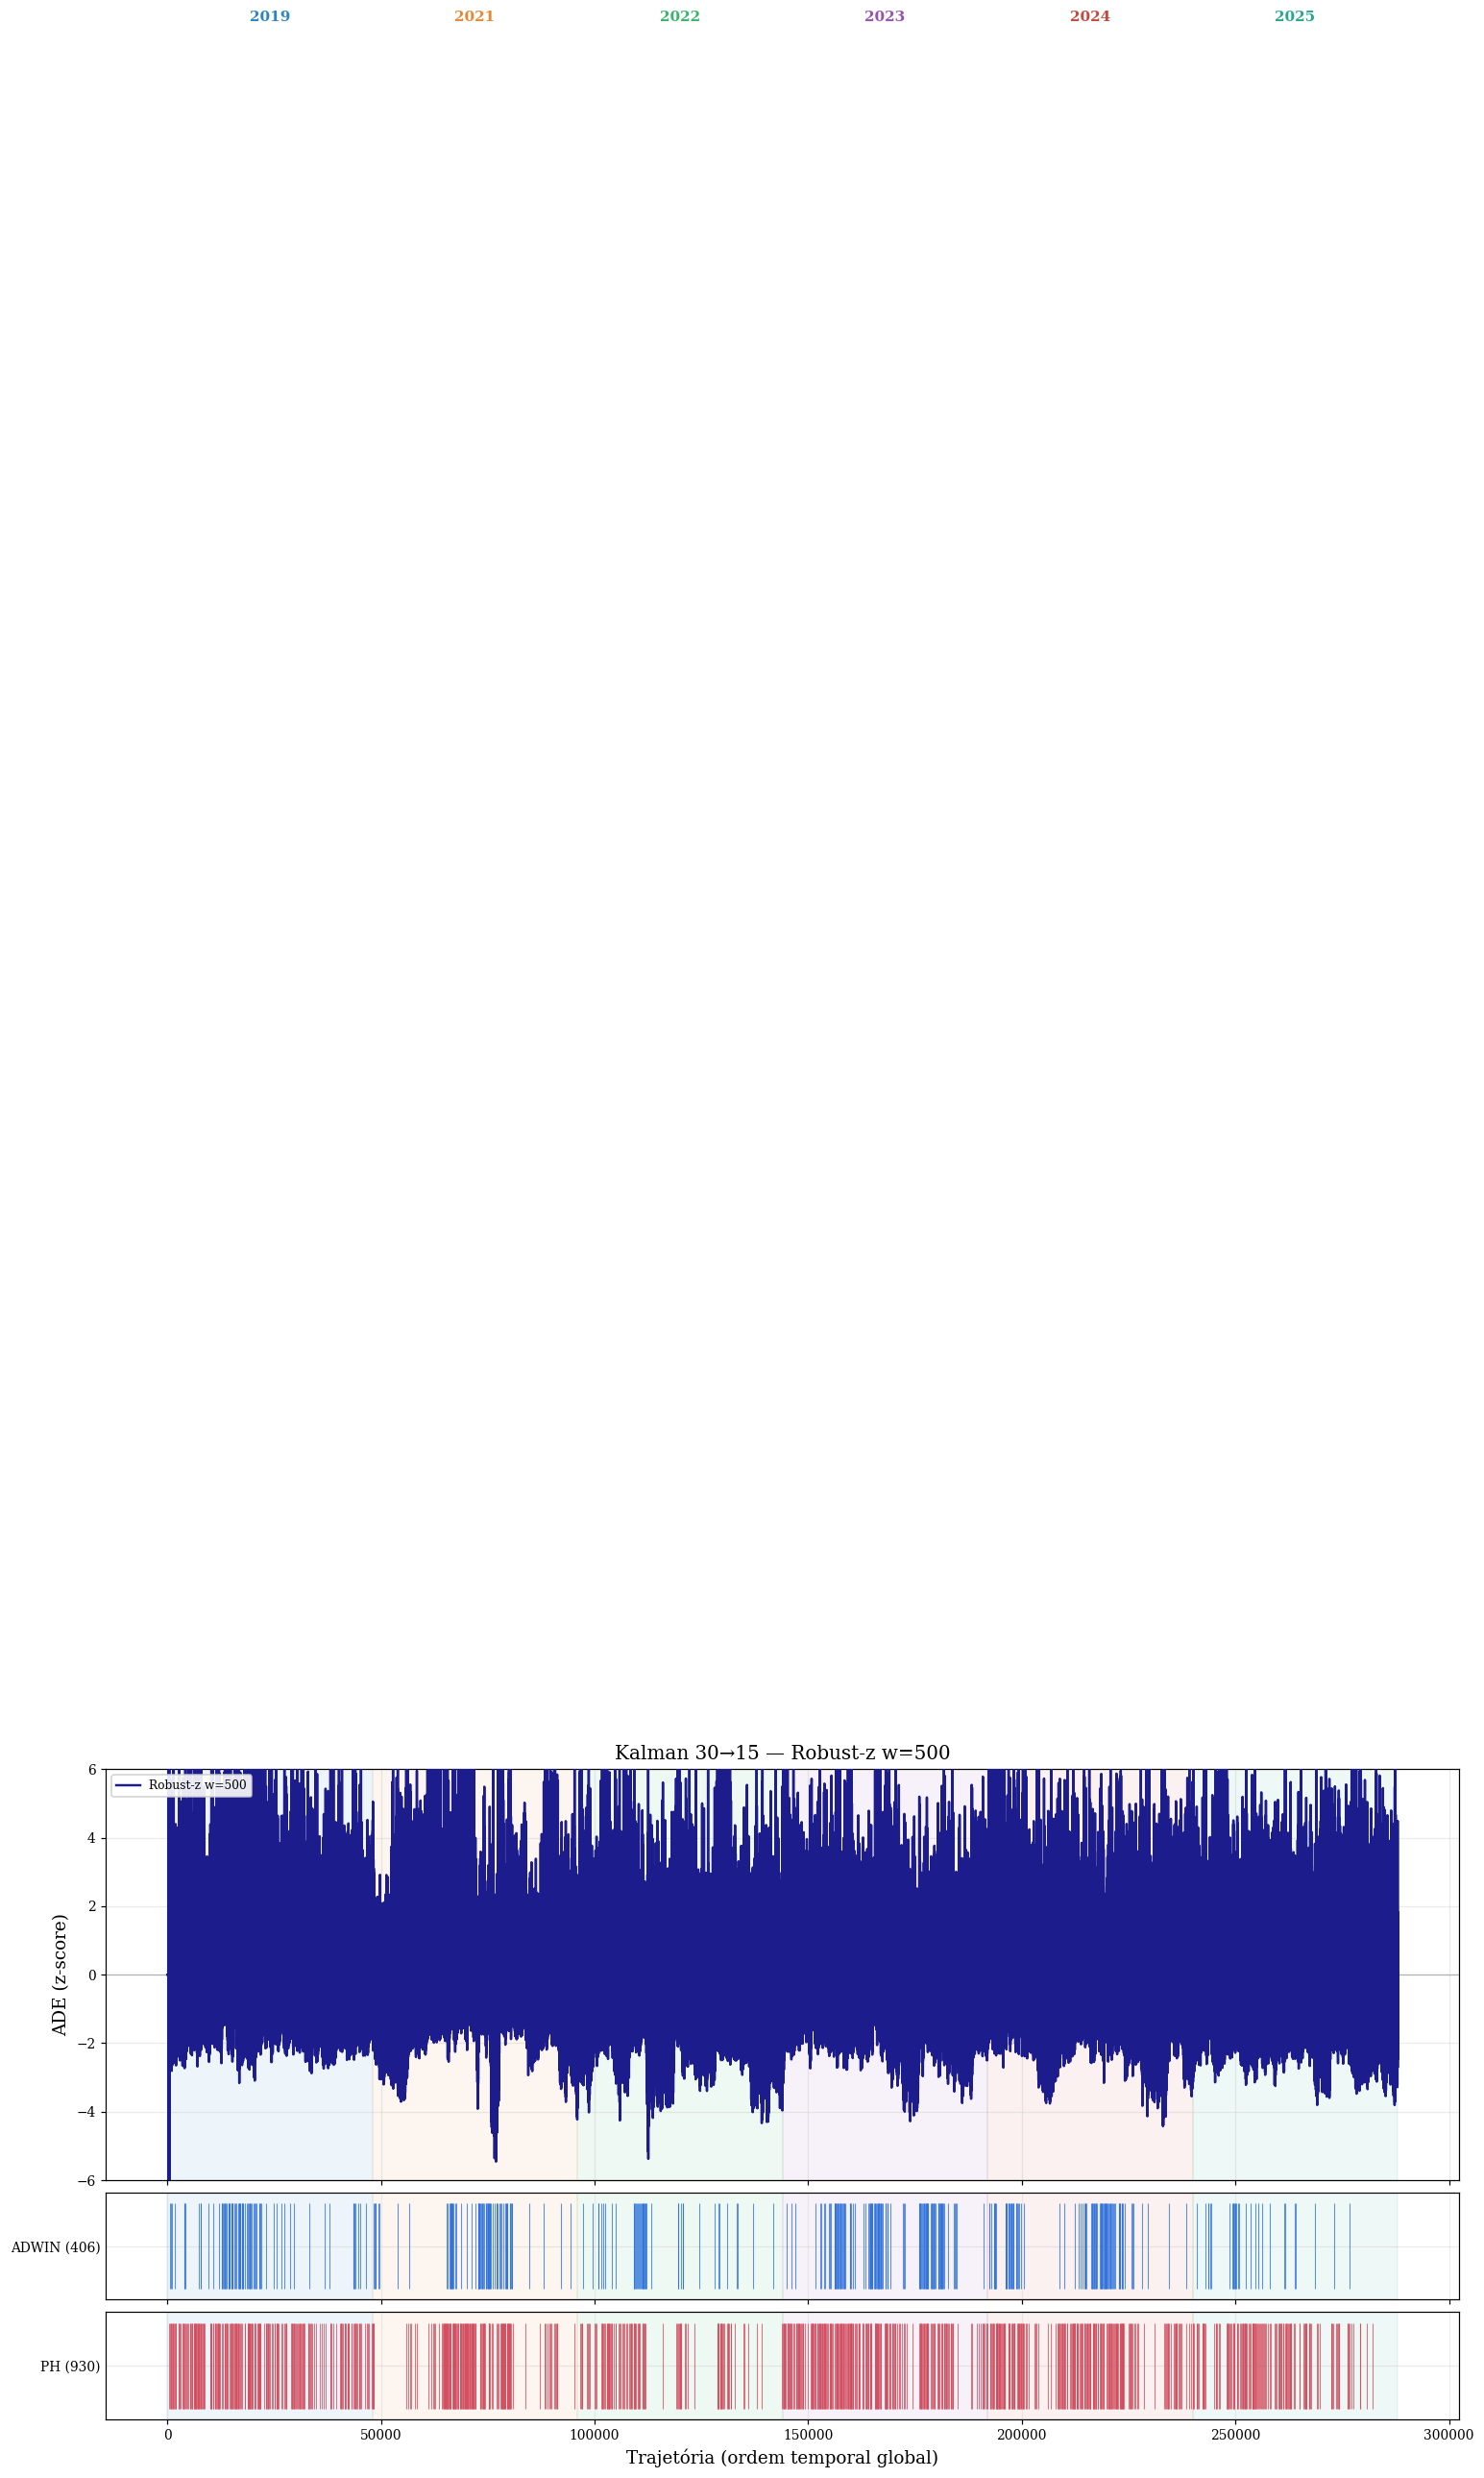
\includegraphics[width=\linewidth]{../mes9_phase1/images/robz_w500/robz_w500_kalman}\caption{\texttt{robz\_w500} --- Kalman.}\end{subfigure}
\caption{\textbf{Robust-z $w$=500.} Janela maior tem performance ligeiramente
         pior que $w$=200 no Seq2Seq (FAR=1{,}000/1k vs. 0{,}604/1k):
         a normaliza\c{c}\~ao adapta-se mais lentamente \`as mudan\c{c}as
         locais.}
\label{fig:m9_p1_g12}
\end{figure}

\subsubsection{Resumo num\'erico Fase 1}

\begin{table}[H]
\centering\small
\begin{tabular}{l r r r r}
\toprule
\textbf{Suavizador} & \textbf{FAR\textsubscript{2019}/1k (S2S)} & \textbf{n\textsubscript{post} (S2S)} & \textbf{FAR\textsubscript{2019}/1k (Kalman)} & \textbf{n\textsubscript{post} (Kalman)} \\
\midrule
\texttt{ctrl}        & 1{,}229 & 256 & 1{,}271 & 324 \\
\textbf{robz\_w200}  & \textbf{0{,}604} & \textbf{85} & \textbf{0{,}542} & \textbf{220} \\
\texttt{robz\_w500}  & 1{,}000 & 221 & 1{,}542 & 332 \\
\texttt{ewma\_a030}  & 3{,}438 & 641 & 2{,}812 & 624 \\
\texttt{ewma\_a020}  & 4{,}708 & 801 & 3{,}500 & 775 \\
\texttt{sma\_w020}   & 5{,}917 & 1\,246 & 5{,}417 & 1\,230 \\
\texttt{med\_w200}   & 8{,}938 (Kalman) & --- & 8{,}938 & 2\,162 \\
\texttt{sma\_w500}   & 9{,}104 (Kalman) & --- & 9{,}104 & 2\,177 \\
\bottomrule
\end{tabular}
\caption{Resumo Fase 1 (ADWIN sobre stream suavizado, ordenado por
         FAR\textsubscript{2019} crescente). Apenas
         \texttt{robz\_w200} reduz a FAR vs.\ controlo; todos os outros
         suavizadores aumentam. Fonte: \texttt{phase1\_results.csv}.}
\label{tab:m9_p1_summary}
\end{table}

% ----------------------------------------------------------------------------
\subsection{Fase 2 --- Grid search 174 configs em tr\^es frentes}
% ----------------------------------------------------------------------------

\subsubsection{Setup}

Tr\^es frentes paralelas de busca em grade, todas com pr\'e-processamento
\texttt{robz\_w200}:

\begin{itemize}[leftmargin=1.4em,itemsep=2pt]
    \item \textbf{Frente A --- ADWIN sobre ADE robz}. Sweep de
          $\delta\!\in\!\{10^{-7},10^{-6},10^{-5},10^{-4}\}$,
          \texttt{min\_window}\,$\in\!\{200, 400, 600, 1000\}$,
          \texttt{cooldown}\,$\in\!\{200, 500, 1000\}$,
          \texttt{max\_window}\,$\in\!\{2000, 5000\}$.
    \item \textbf{Frente B --- Page-Hinkley agregado por janelas}.
          PH aplicado \`a m\'edia trimmed-mean em janelas de
          $N\!\in\!\{50, 100, 200, 500\}$;
          $K_\text{thr}\!\in\!\{20, 30, 50\}$, $\delta\!\in\!\{0{,}5;1{,}0;2{,}0\}$.
    \item \textbf{Frente C --- KSWIN}. $\alpha\!\in\!\{10^{-5},10^{-4},10^{-3}\}$,
          \texttt{window\_size}\,$\in\!\{200, 500, 1000\}$,
          \texttt{stat\_size}\,$\in\!\{50, 100\}$.
\end{itemize}

Total: 174 configs $\times$ 2 modelos.

\subsubsection{Heatmaps das tr\^es frentes (sele\c{c}\~ao posterior)}

\begin{figure}[H]
\centering
\begin{subfigure}[b]{0.48\textwidth}\centering
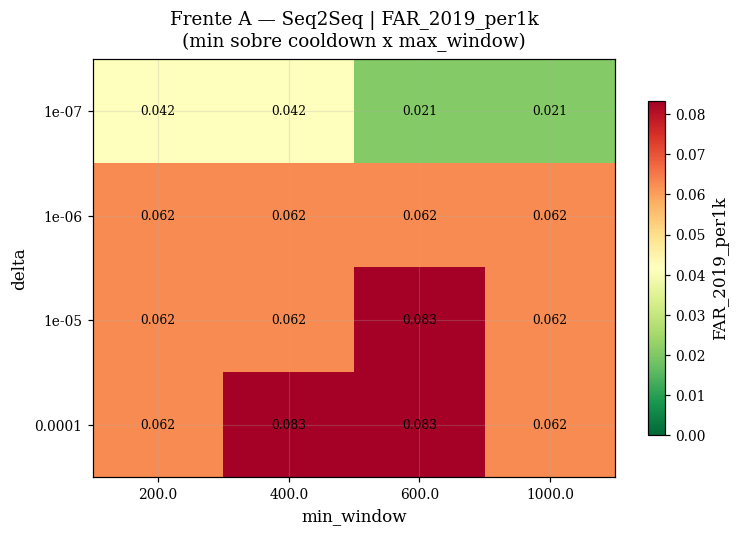
\includegraphics[width=\linewidth]{../mes9_phase2/images/frente_A/heatmap_FAR_2019_per1k_seq2seq}
\caption{Frente A --- FAR\textsubscript{2019} S2S.}\end{subfigure}\hfill
\begin{subfigure}[b]{0.48\textwidth}\centering
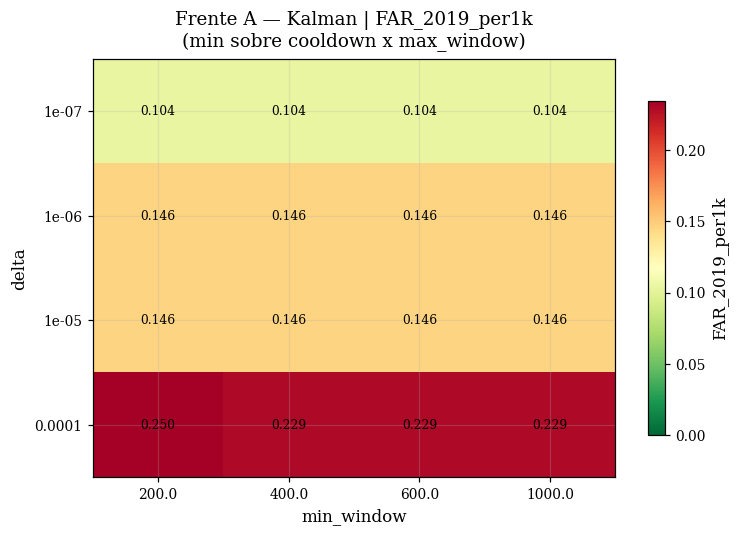
\includegraphics[width=\linewidth]{../mes9_phase2/images/frente_A/heatmap_FAR_2019_per1k_kalman}
\caption{Frente A --- FAR\textsubscript{2019} Kalman.}\end{subfigure}

\vspace{0.4em}
\begin{subfigure}[b]{0.48\textwidth}\centering
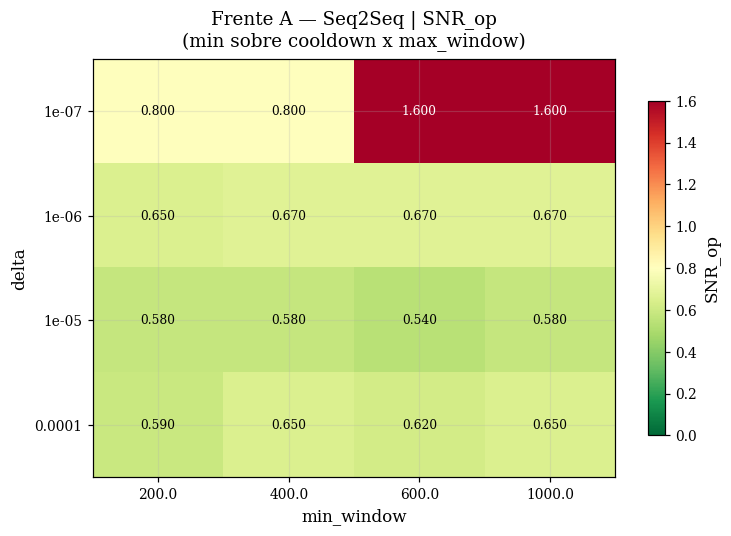
\includegraphics[width=\linewidth]{../mes9_phase2/images/frente_A/heatmap_SNR_op_seq2seq}
\caption{Frente A --- SNR\textsubscript{op} S2S.}\end{subfigure}\hfill
\begin{subfigure}[b]{0.48\textwidth}\centering
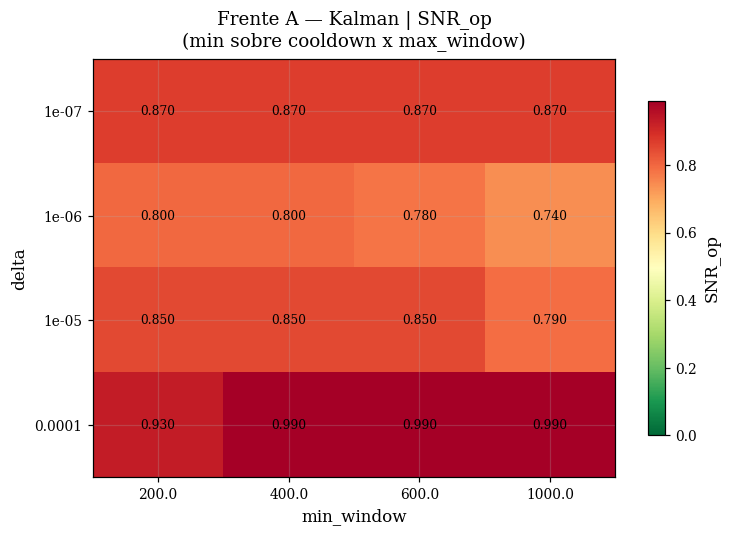
\includegraphics[width=\linewidth]{../mes9_phase2/images/frente_A/heatmap_SNR_op_kalman}
\caption{Frente A --- SNR\textsubscript{op} Kalman.}\end{subfigure}

\vspace{0.4em}
\begin{subfigure}[b]{0.48\textwidth}\centering
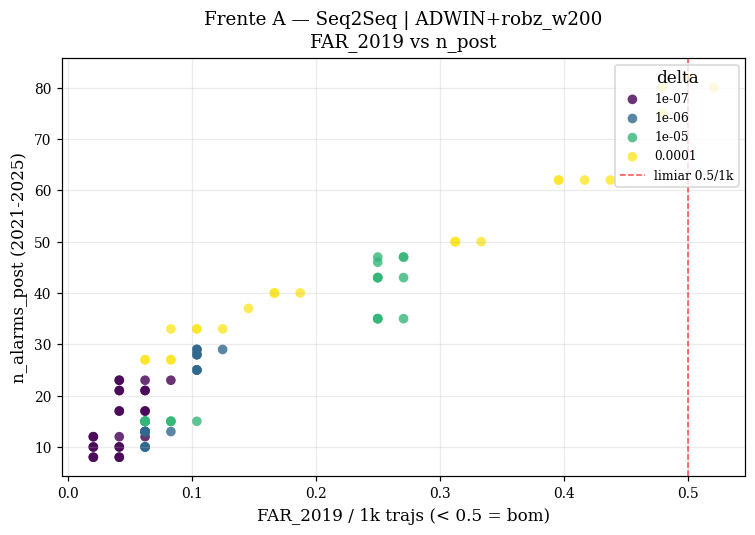
\includegraphics[width=\linewidth]{../mes9_phase2/images/frente_A/scatter_seq2seq}
\caption{Frente A --- scatter S2S.}\end{subfigure}\hfill
\begin{subfigure}[b]{0.48\textwidth}\centering
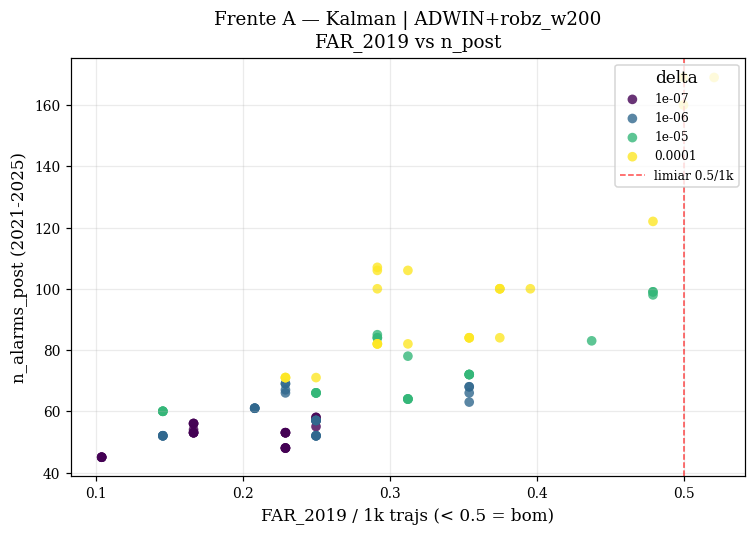
\includegraphics[width=\linewidth]{../mes9_phase2/images/frente_A/scatter_kalman}
\caption{Frente A --- scatter Kalman.}\end{subfigure}
\caption{\textbf{Frente A (ADWIN+robz)}: heatmaps FAR e SNR e
         scatter FAR vs.\ $n_\text{post}$. \emph{Menor FAR S2S:}
         $\delta=10^{-7}$, mw=1000, xw=5000 --- FAR=0{,}021/1k, mas
         cobertura 3/5 (n\~ao dispara em 2024--2025).
         \emph{Config adotada (S2S):} $\delta=10^{-7}$, mw=600, cd=200,
         xw=2000 --- FAR=0{,}042/1k, $n_\text{post}=23$, year\_cov=5/5.
         \emph{Melhor Kalman:} $\delta=10^{-7}$, mw=200, cd=1000,
         xw=5000 --- FAR=0{,}104/1k.}
\label{fig:m9_p2_A}
\end{figure}

\begin{figure}[H]
\centering
\begin{subfigure}[b]{0.48\textwidth}\centering

\includegraphics[width=\linewidth]{../mes9_phase2/images/frente_B/heatmap_FAR_2019_per1k_seq2seq}
\caption{Frente B --- FAR\textsubscript{2019} S2S.}\end{subfigure}\hfill
\begin{subfigure}[b]{0.48\textwidth}\centering

\includegraphics[width=\linewidth]{../mes9_phase2/images/frente_B/heatmap_FAR_2019_per1k_kalman}
\caption{Frente B --- FAR\textsubscript{2019} Kalman.}\end{subfigure}

\vspace{0.4em}
\begin{subfigure}[b]{0.48\textwidth}\centering

\includegraphics[width=\linewidth]{../mes9_phase2/images/frente_B/heatmap_SNR_op_seq2seq}
\caption{Frente B --- SNR\textsubscript{op} S2S.}\end{subfigure}\hfill
\begin{subfigure}[b]{0.48\textwidth}\centering

\includegraphics[width=\linewidth]{../mes9_phase2/images/frente_B/heatmap_SNR_op_kalman}
\caption{Frente B --- SNR\textsubscript{op} Kalman.}\end{subfigure}

\vspace{0.4em}
\begin{subfigure}[b]{0.48\textwidth}\centering

\includegraphics[width=\linewidth]{../mes9_phase2/images/frente_B/scatter_seq2seq}
\caption{Frente B --- scatter S2S.}\end{subfigure}\hfill
\begin{subfigure}[b]{0.48\textwidth}\centering

\includegraphics[width=\linewidth]{../mes9_phase2/images/frente_B/scatter_kalman}
\caption{Frente B --- scatter Kalman.}\end{subfigure}
\caption{\textbf{Frente B (PH agregado)}: a melhor config S2S
         (N=50, K=50, $\delta$=2{,}0) atinge FAR=0/1k mas
         year\_coverage=1/5 (apenas 2021). Limita\c{c}\~ao estrutural
         do PH agregado para drift gradual --- ver
         Fase 4 (Se\c{c}\~ao~\ref{sec:m9_p4}).}
\label{fig:m9_p2_B}
\end{figure}

\begin{figure}[H]
\centering
\begin{subfigure}[b]{0.48\textwidth}\centering

\includegraphics[width=\linewidth]{../mes9_phase2/images/frente_C/heatmap_FAR_2019_per1k_seq2seq}
\caption{Frente C --- FAR\textsubscript{2019} S2S.}\end{subfigure}\hfill
\begin{subfigure}[b]{0.48\textwidth}\centering

\includegraphics[width=\linewidth]{../mes9_phase2/images/frente_C/heatmap_FAR_2019_per1k_kalman}
\caption{Frente C --- FAR\textsubscript{2019} Kalman.}\end{subfigure}

\vspace{0.4em}
\begin{subfigure}[b]{0.48\textwidth}\centering

\includegraphics[width=\linewidth]{../mes9_phase2/images/frente_C/heatmap_SNR_op_seq2seq}
\caption{Frente C --- SNR\textsubscript{op} S2S.}\end{subfigure}\hfill
\begin{subfigure}[b]{0.48\textwidth}\centering

\includegraphics[width=\linewidth]{../mes9_phase2/images/frente_C/heatmap_SNR_op_kalman}
\caption{Frente C --- SNR\textsubscript{op} Kalman.}\end{subfigure}

\vspace{0.4em}
\begin{subfigure}[b]{0.48\textwidth}\centering

\includegraphics[width=\linewidth]{../mes9_phase2/images/frente_C/scatter_seq2seq}
\caption{Frente C --- scatter S2S.}\end{subfigure}\hfill
\begin{subfigure}[b]{0.48\textwidth}\centering

\includegraphics[width=\linewidth]{../mes9_phase2/images/frente_C/scatter_kalman}
\caption{Frente C --- scatter Kalman.}\end{subfigure}
\caption{\textbf{Frente C (KSWIN)}: \emph{melhor} config atinge
         FAR=0{,}438/1k (S2S), acima do limiar de admissibilidade
         0{,}20/1k. SNR\textsubscript{op}=0{,}77 (sub-unit\'ario, indica
         que h\'a mais alarmes em 2019 proporcionalmente do que no
         per\'iodo p\'os-2019). KSWIN \'e \textbf{exclu\'ido} do
         ensemble final.}
\label{fig:m9_p2_C}
\end{figure}

\subsubsection{Top-5 streams das tr\^es frentes}

\begin{figure}[H]
\centering
\begin{subfigure}[b]{0.48\textwidth}\centering
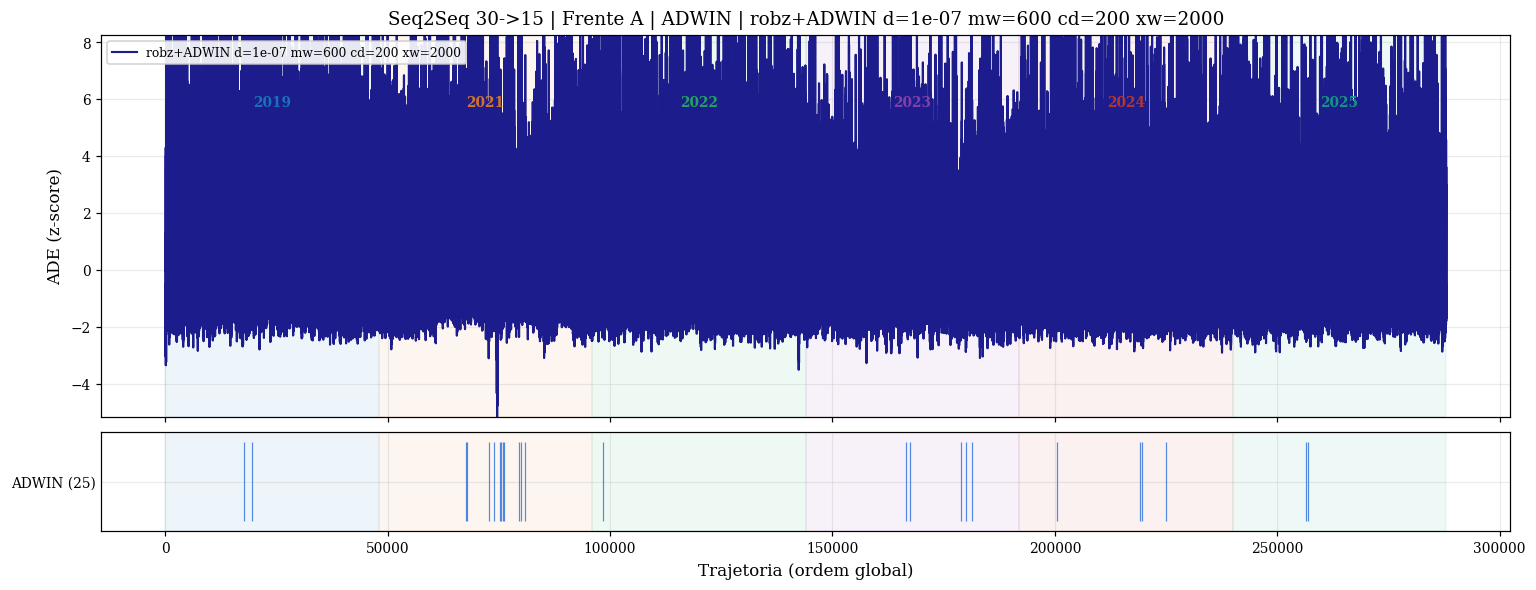
\includegraphics[width=\linewidth]{../mes9_phase2/images/frente_A/A_d1e-07_mw600_cd200_xw2000_seq2seq_stream}
\caption{A: $\delta$=$10^{-7}$, mw=600, cd=200, xw=2000 (ADWINLite, refer\^encia).}\end{subfigure}\hfill
\begin{subfigure}[b]{0.48\textwidth}\centering
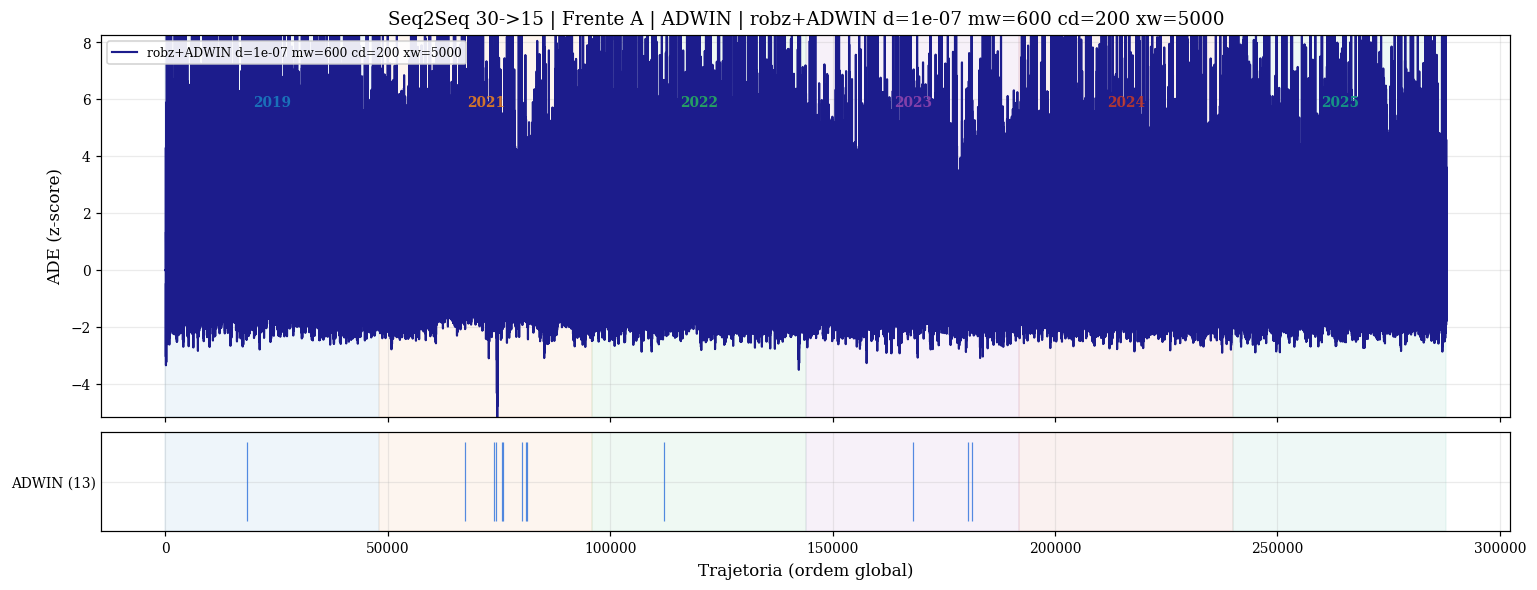
\includegraphics[width=\linewidth]{../mes9_phase2/images/frente_A/A_d1e-07_mw600_cd200_xw5000_seq2seq_stream}
\caption{A: $\delta$=$10^{-7}$, mw=600, cd=200, xw=5000.}\end{subfigure}

\vspace{0.3em}
\begin{subfigure}[b]{0.48\textwidth}\centering
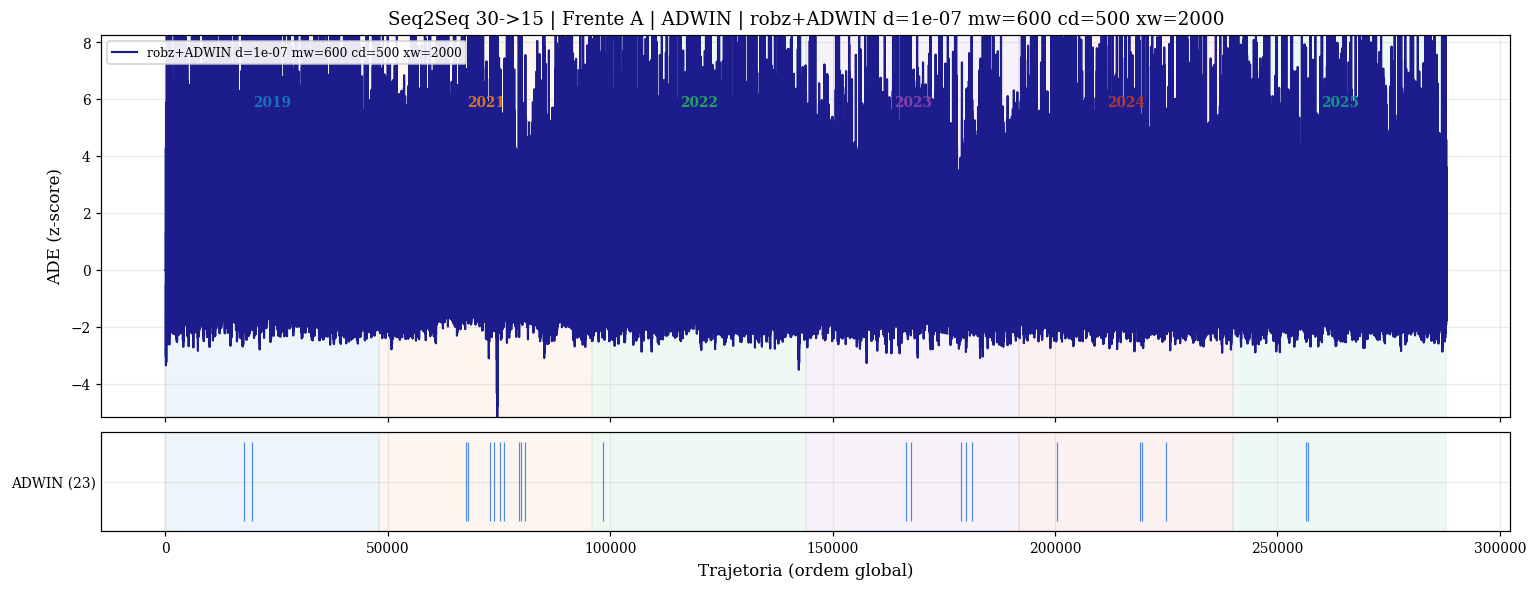
\includegraphics[width=\linewidth]{../mes9_phase2/images/frente_A/A_d1e-07_mw600_cd500_xw2000_seq2seq_stream}
\caption{A: $\delta$=$10^{-7}$, mw=600, cd=500, xw=2000.}\end{subfigure}\hfill
\begin{subfigure}[b]{0.48\textwidth}\centering
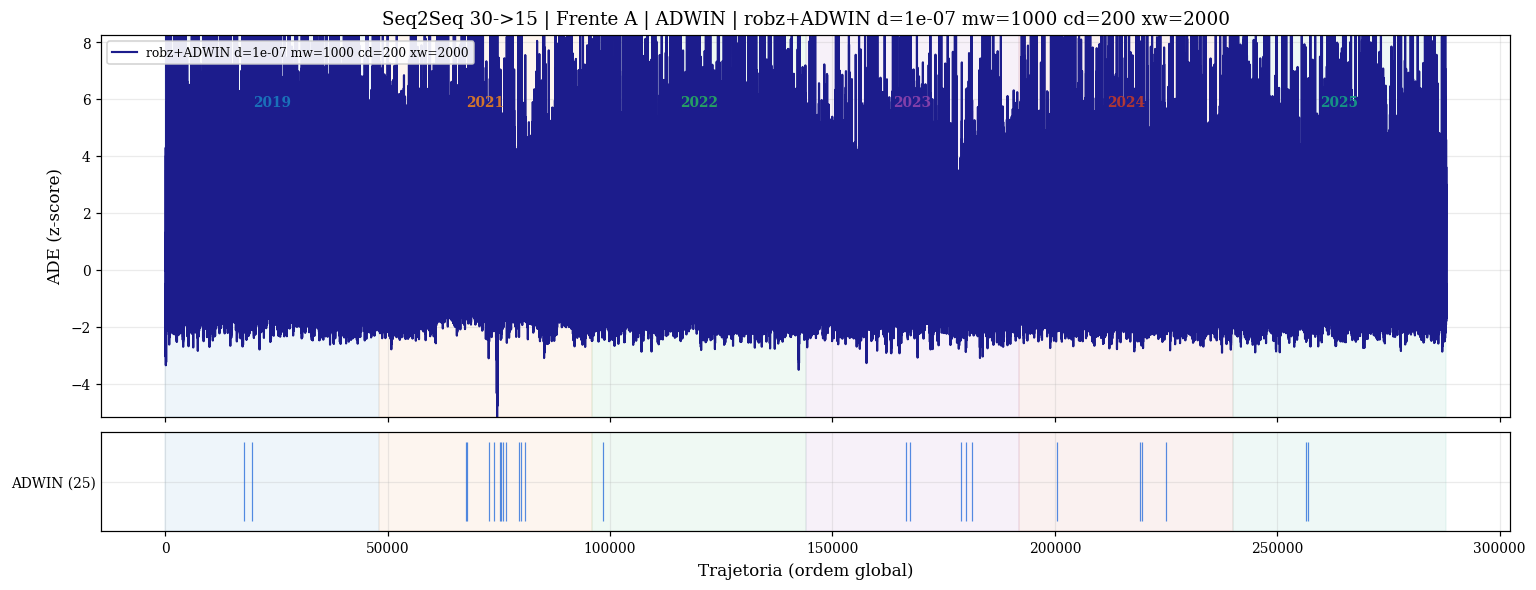
\includegraphics[width=\linewidth]{../mes9_phase2/images/frente_A/A_d1e-07_mw1000_cd200_xw2000_seq2seq_stream}
\caption{A: $\delta$=$10^{-7}$, mw=1000, cd=200, xw=2000.}\end{subfigure}

\vspace{0.3em}
\begin{subfigure}[b]{0.7\textwidth}\centering
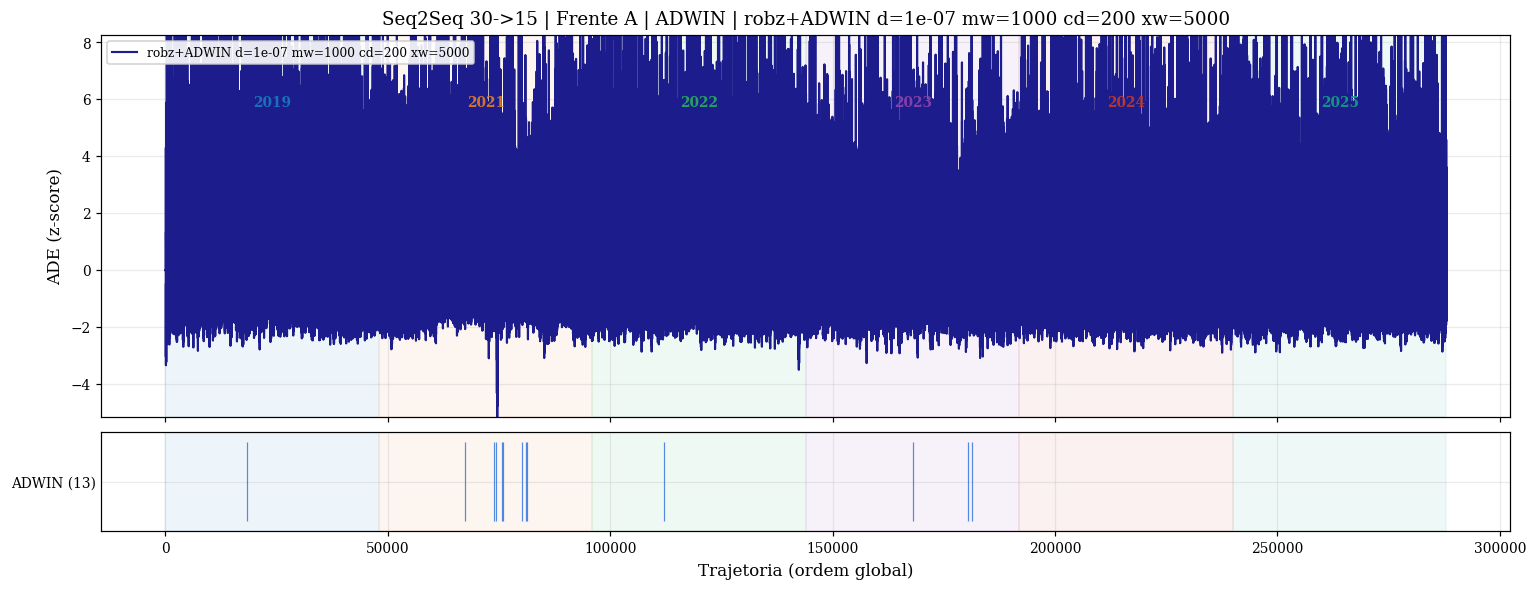
\includegraphics[width=\linewidth]{../mes9_phase2/images/frente_A/A_d1e-07_mw1000_cd200_xw5000_seq2seq_stream}
\caption{A: $\delta$=$10^{-7}$, mw=1000, cd=200, xw=5000.}\end{subfigure}
\caption{\textbf{Frente A --- top-5 streams Seq2Seq.} A escolha
         final (config \#1) maximiza
         (FAR\textsubscript{2019}\,$\to$\,$\min$, year\_cov\,$\to\,5$,
         $n_\text{post}\,$razo\'avel). Linhas verticais = alarmes ADWIN.}
\label{fig:m9_grid_streams_a}
\end{figure}

\begin{figure}[H]
\centering
\begin{subfigure}[b]{0.48\textwidth}\centering
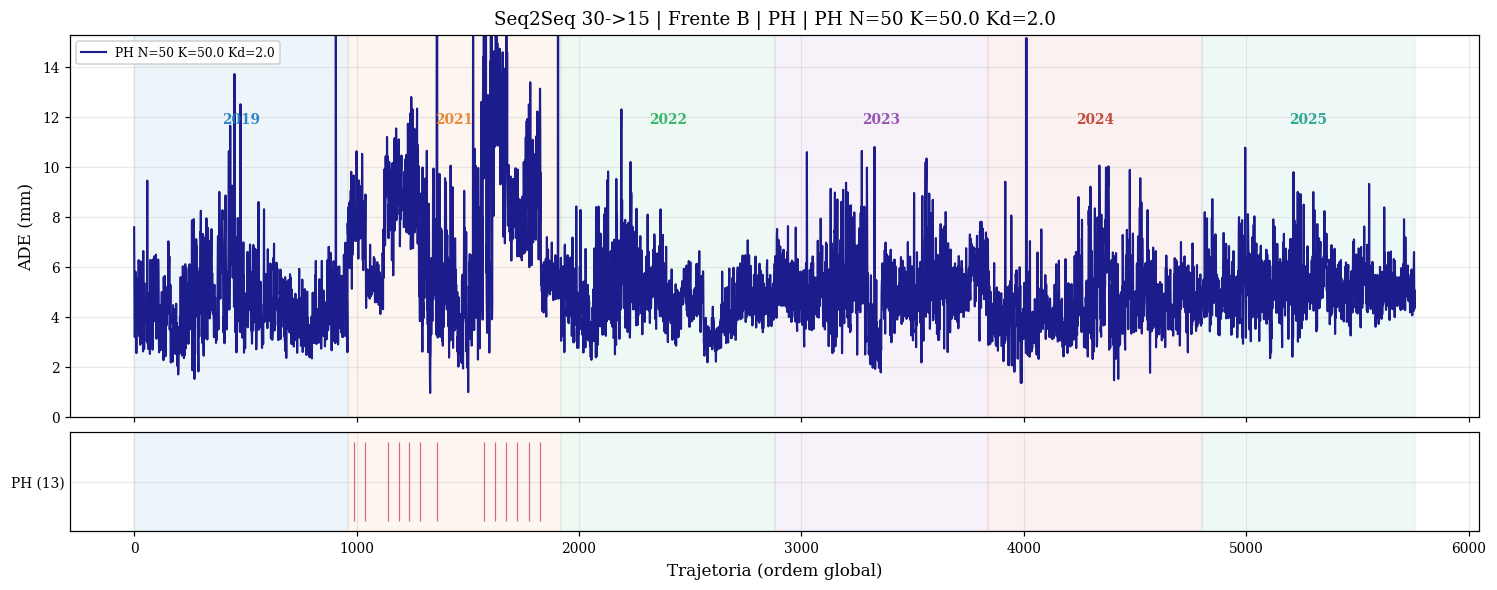
\includegraphics[width=\linewidth]{../mes9_phase2/images/frente_B/B_N50_K50_d2.0_seq2seq_stream}
\caption{B: N=50, K=50, $\delta$=2{,}0 \textbf{(\#1)}.}\end{subfigure}\hfill
\begin{subfigure}[b]{0.48\textwidth}\centering
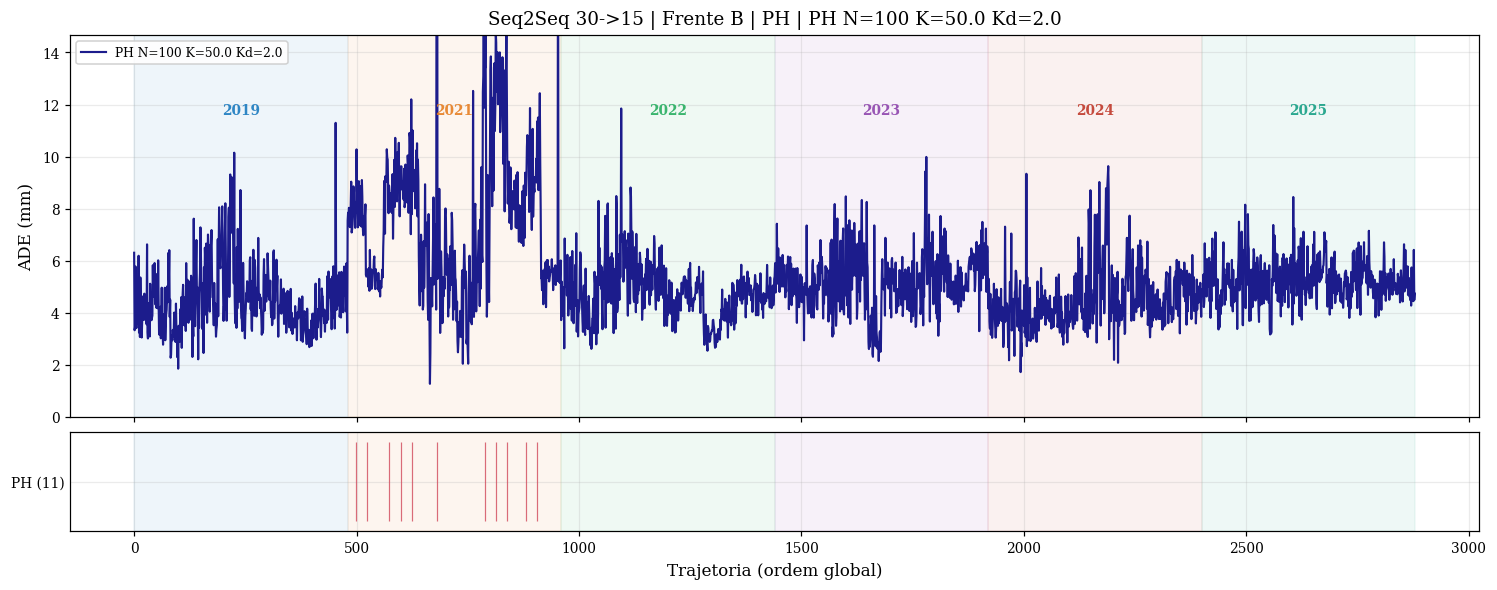
\includegraphics[width=\linewidth]{../mes9_phase2/images/frente_B/B_N100_K50_d2.0_seq2seq_stream}
\caption{B: N=100, K=50, $\delta$=2{,}0.}\end{subfigure}

\vspace{0.3em}
\begin{subfigure}[b]{0.48\textwidth}\centering
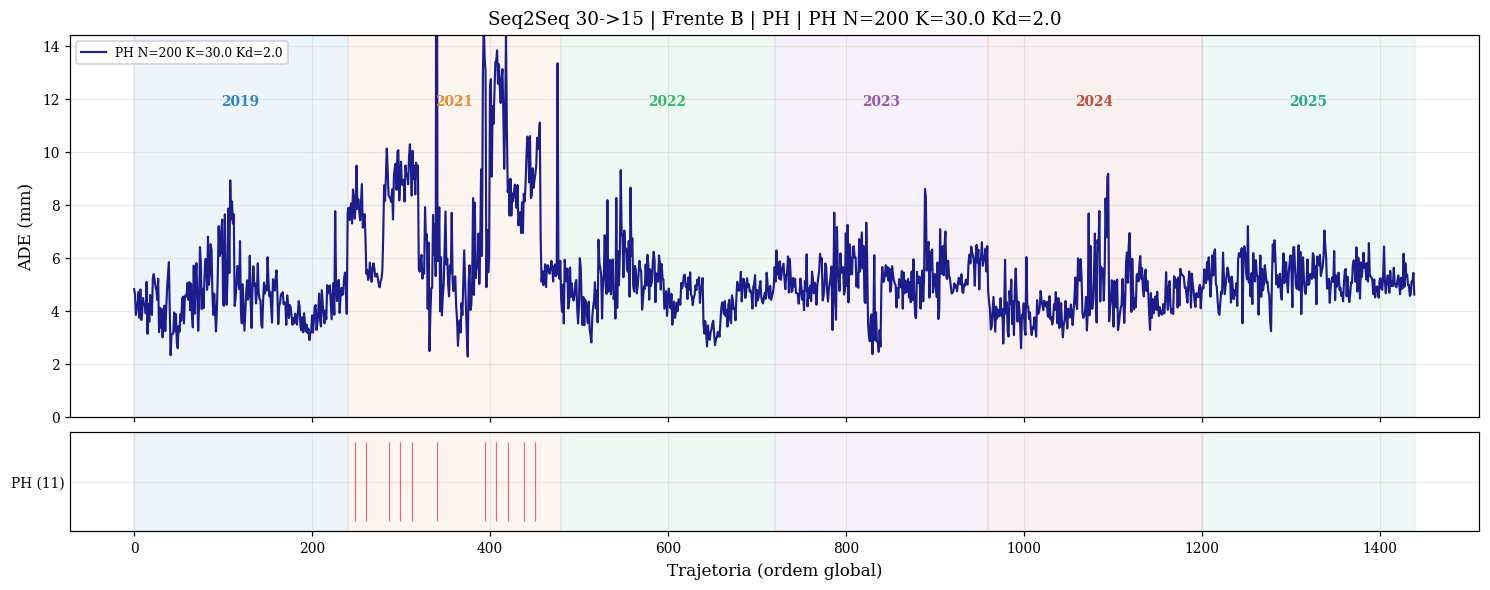
\includegraphics[width=\linewidth]{../mes9_phase2/images/frente_B/B_N200_K30_d2.0_seq2seq_stream}
\caption{B: N=200, K=30, $\delta$=2{,}0.}\end{subfigure}\hfill
\begin{subfigure}[b]{0.48\textwidth}\centering
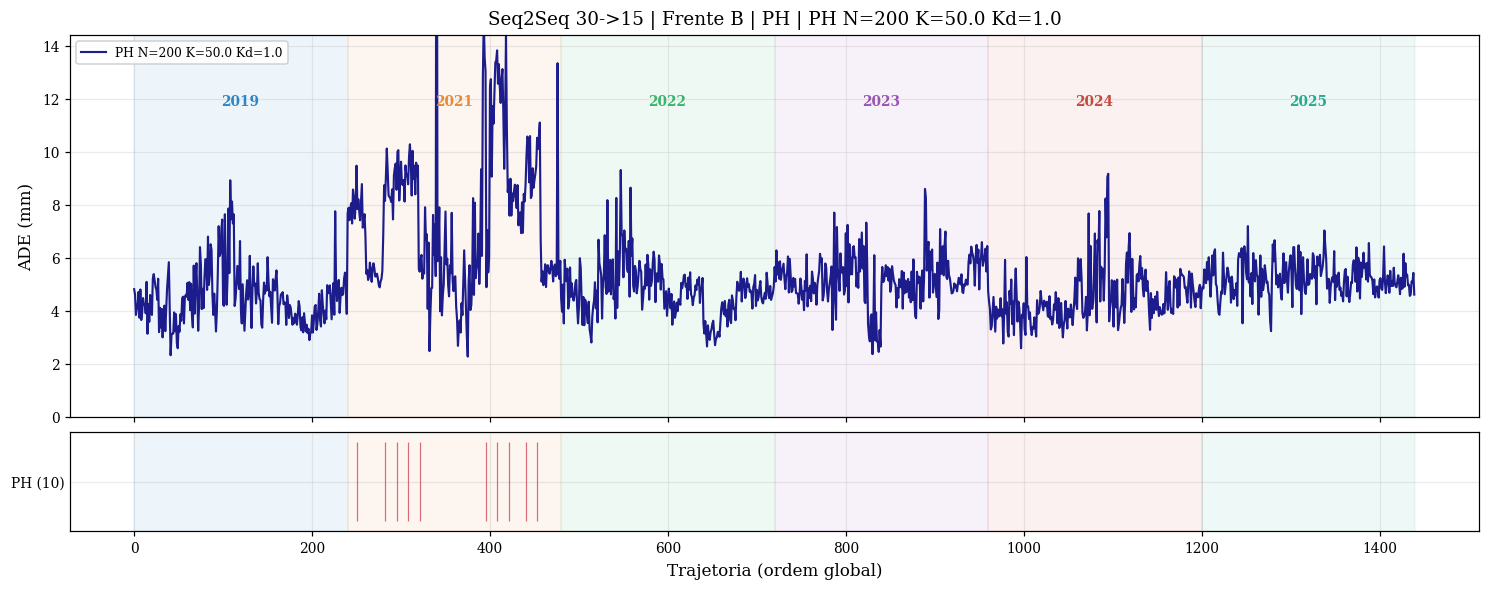
\includegraphics[width=\linewidth]{../mes9_phase2/images/frente_B/B_N200_K50_d1.0_seq2seq_stream}
\caption{B: N=200, K=50, $\delta$=1{,}0.}\end{subfigure}

\vspace{0.3em}
\begin{subfigure}[b]{0.7\textwidth}\centering
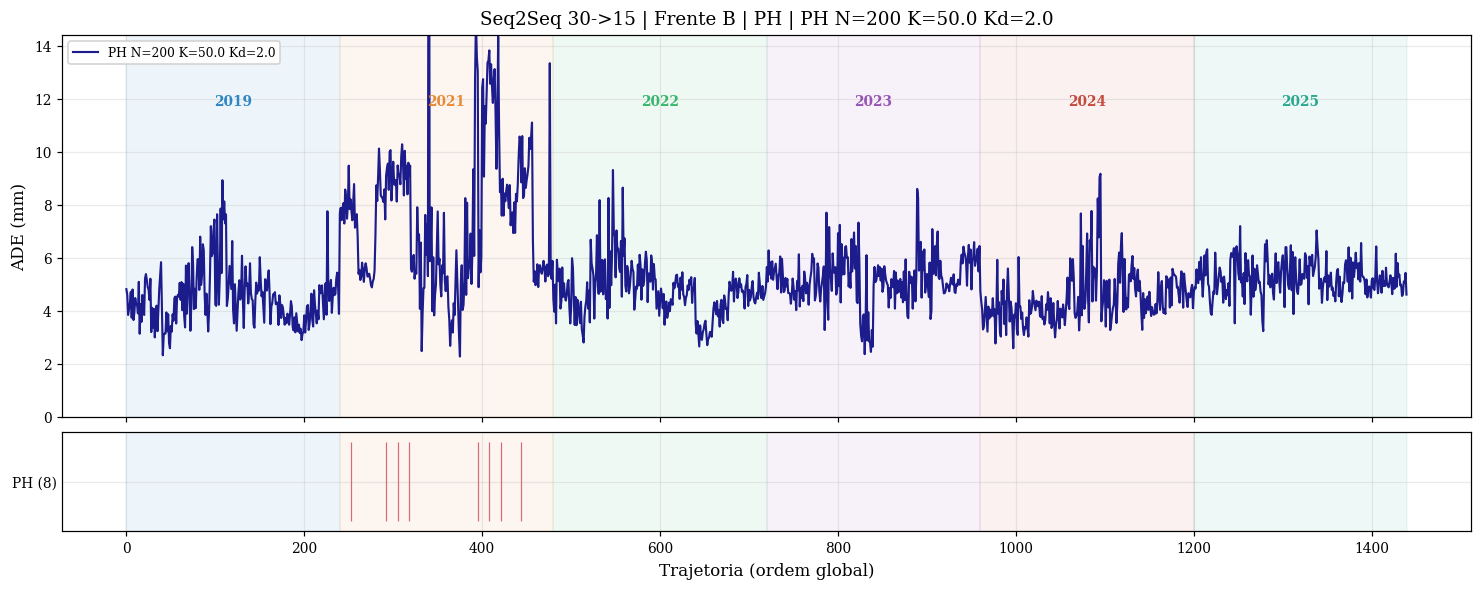
\includegraphics[width=\linewidth]{../mes9_phase2/images/frente_B/B_N200_K50_d2.0_seq2seq_stream}
\caption{B: N=200, K=50, $\delta$=2{,}0.}\end{subfigure}
\caption{\textbf{Frente B --- top-5 streams Seq2Seq.} A config \#1
         (N=50) \'e a \'unica que dispara em 2021 com FAR=0/1k em 2019.
         As demais variantes ou n\~ao disparam ou disparam tamb\'em em
         2019. Padr\~ao: PH agregado deteta exclusivamente a
         transi\c{c}\~ao 2019$\to$2021 e n\~ao deteta drifts em
         2022--2025.}
\label{fig:m9_grid_streams_b}
\end{figure}

\subsubsection{Padr\~ao por ano nas tr\^es frentes}

\begin{table}[H]
\centering\small
\begin{tabular}{l r r r r r r r}
\toprule
\textbf{Frente / config} & \textbf{FAR/1k} & \textbf{SNR\textsubscript{op}} & \textbf{n\textsubscript{2021}} & \textbf{n\textsubscript{2022}} & \textbf{n\textsubscript{2023}} & \textbf{n\textsubscript{2024}} & \textbf{n\textsubscript{2025}} \\
\midrule
A adotada (S2S)    & 0{,}042 & 2{,}30 & 11 & 1 & 5 & 4 & 2 \\
A adotada (Kalman) & 0{,}104 & 1{,}80 & 14 & 11 & 10 & 9 & 1 \\
B best (S2S)       & 0{,}000 & 9999 & 12 & 0 & 0 & 0 & 0 \\
B best (Kalman)    & 0{,}000 & 9999 & 9 & 0 & 0 & 0 & 0 \\
C best (S2S)       & 0{,}438 & 0{,}77 & 22 & 13 & 17 & 15 & 14 \\
C best (Kalman)    & 0{,}583 & 0{,}75 & 28 & 19 & 22 & 22 & 14 \\
\bottomrule
\end{tabular}
\caption{Padr\~ao de detec\c{c}\~ao por ano nas tr\^es frentes (melhor
         config de cada). \emph{Frente A:} cobertura 5/5 anos.
         \emph{Frente B:} cobertura 1/5 (s\'o 2021) --- limita\c{c}\~ao
         estrutural. \emph{Frente C (KSWIN):} cobertura 5/5 mas
         FAR\,>\,0{,}20/1k --- inadmiss\'ivel. Fonte:
         \texttt{phase2\_results.csv}.}
\label{tab:m9_p2_byyear}
\end{table}

% ----------------------------------------------------------------------------
\subsection{Fase 3 --- Ensemble temporal AND/OR dois andares}
% ----------------------------------------------------------------------------

\subsubsection{Config do ensemble}

\begin{table}[H]
\centering\small
\begin{tabular}{l l l}
\toprule
\textbf{Canal} & \textbf{Detector} & \textbf{Config} \\
\midrule
ADWIN\_S2S (espinha) & ADWIN+robz $w$=200 & $\delta\!=\!10^{-7}$, mw=600, cd=200, xw=2000 \\
PH\_agg (validador)  & PH N=50 trimmed-mean & K=50, $\delta\!=\!2{,}0$ \\
Kalman (OR-only)     & ADWIN+robz $w$=200 & $\delta\!=\!10^{-7}$, mw=200, cd=1000, xw=5000 \\
\bottomrule
\end{tabular}
\caption{Componentes do ensemble. \emph{Tier 1 CONFIRMED:}
         AND(ADWIN\_S2S, PH\_agg) com janela de coincid\^encia
         $W$\,=\,200 trajs e \texttt{retrain\_debounce}\,=\,5000.
         \emph{Tier 2 SUSPECTED:} OR(ADWIN\_S2S, Kalman).
         O Kalman nunca entra no AND.}
\label{tab:m9_p3_config}
\end{table}

\subsubsection{Resultados}

\begin{table}[H]
\centering\small
\begin{tabular}{l r r r r}
\toprule
\textbf{Canal} & \textbf{n\textsubscript{alarms}} & \textbf{FAR\textsubscript{2019}/1k} & \textbf{n\textsubscript{post}} & \textbf{Anos cobertos} \\
\midrule
CONFIRMED (W=200)  & 0 & 0{,}000 & 0 & 0/5 \\
SUSPECTED (OR)     & 75 & 0{,}146 & 68 & \textbf{5/5} \\
ADWIN standalone   & 25 & 0{,}042 & 23 & 5/5 \\
PH standalone      & 12 & 0{,}000 & 12 & 1/5 (s\'o 2021) \\
Kalman standalone  & 50 & 0{,}104 & 45 & 5/5 \\
\bottomrule
\end{tabular}
\caption{Resultados Fase 3 (288\,k trajs). Com W=200, o canal
         CONFIRMED produz \textbf{0 alarmes}: ADWIN e PH operam em
         escalas temporais distintas. SUSPECTED OR cobre 5/5 anos mas
         com FAR\,>\,0{,}10/1k. Fonte: \texttt{phase3\_results.csv}.}
\label{tab:m9_p3_results}
\end{table}

\subsubsection{Sweep $W_\text{coincidence}$ e descoberta estrutural}

\begin{table}[H]
\centering\small
\begin{tabular}{r r r r}
\toprule
\textbf{$W_\text{coincidence}$ (trajs)} & \textbf{n\textsubscript{confirmed}} & \textbf{FAR\textsubscript{2019}/1k} & \textbf{SNR\textsubscript{op}} \\
\midrule
50    & 0 & 0{,}000 & 0 \\
100   & 0 & 0{,}000 & 0 \\
200   & 0 & 0{,}000 & 0 \\
500   & 1 & 0{,}000 & 9999 \\
1000  & 1 & 0{,}000 & 9999 \\
\bottomrule
\end{tabular}
\caption{Sweep de janela de coincid\^encia (Fase 3). W=500 \'e o m\'inimo
         para coincid\^encia ($\Delta_{\min}$=214 impede coincid\^encia com
         W$\leq$200): produz 1 alarme CONFIRMED (em 2021) com
         FAR=0/1k. A Fase 4 estende este sweep e mostra que mesmo W=10000
         ($\sim$2{,}5 meses operacionais) s\'o produz 4 alarmes em 2 anos ---
         \textbf{inviabilidade estrutural}. Fonte:
         \texttt{W\_infeasibility\_sweep.csv}.}
\label{tab:m9_p3_sweep}
\end{table}

\begin{figure}[H]
\centering
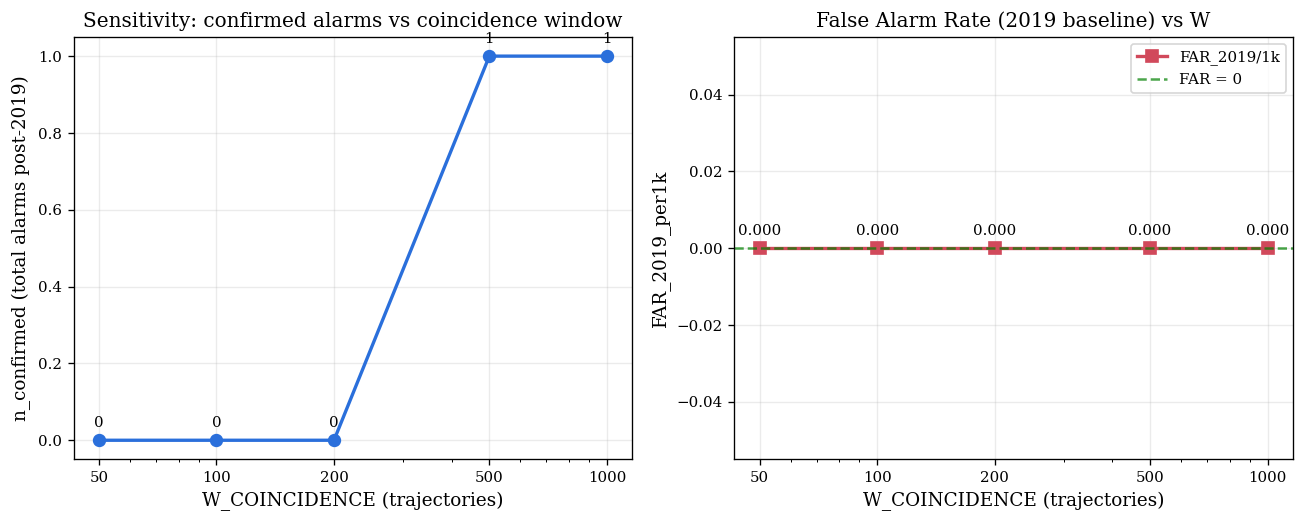
\includegraphics[width=0.85\linewidth]{coincidence_sweep}
\caption{\textbf{Coincidence sweep (Fase 3)} --- $n_\text{confirmed}$
         e FAR vs.\ $W$. O patamar em $n_\text{confirmed}\!\geq\!1$ apenas
         para $W\!\geq\!500$ \'e a assinatura da limita\c{c}\~ao estrutural:
         ADWIN e PH\_agg estao demasiadamente distantes no tempo (Fase 4
         quantifica $\Delta_{\min}\!=\!214$).}
\label{fig:m9_coincidence_sweep}
\end{figure}

\begin{figure}[H]
\centering
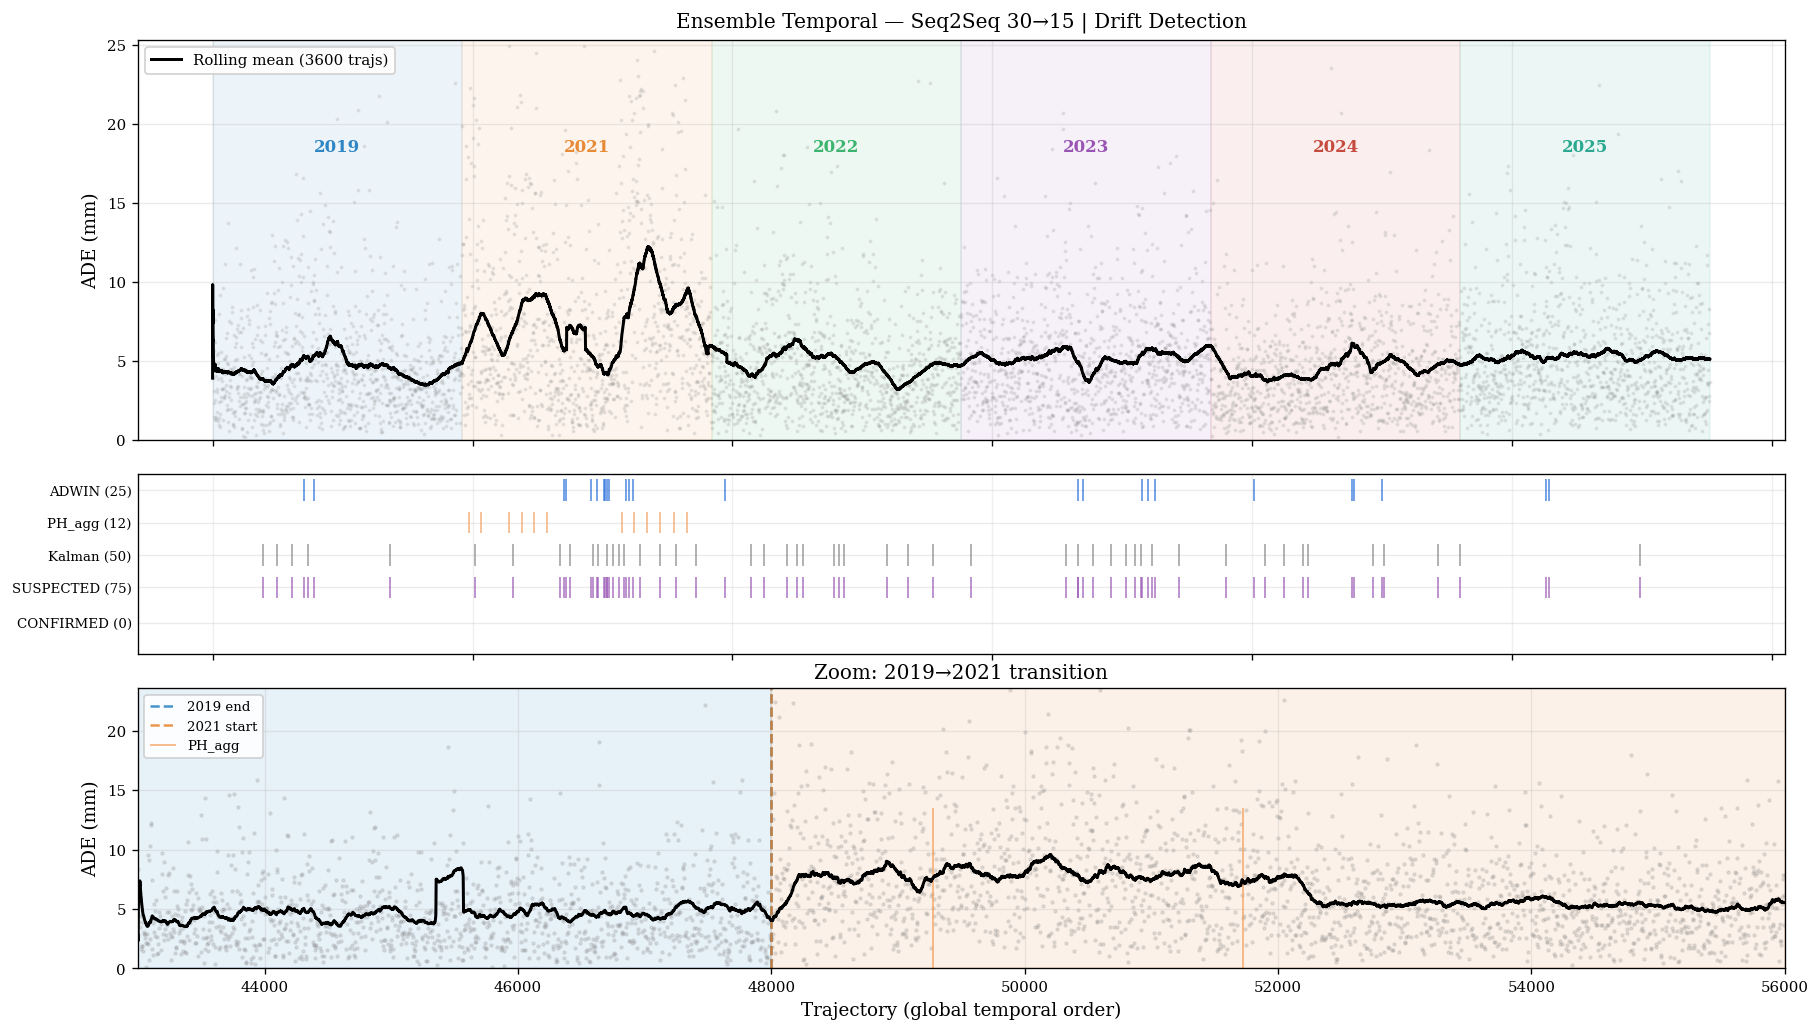
\includegraphics[width=0.95\linewidth]{ensemble_stream_seq2seq}
\caption{\textbf{Stream completo Seq2Seq com 3 canais (Fase 3).}
         Painel superior: alarmes ADWIN\_S2S (azul). Painel meio:
         alarmes PH\_agg (vermelho). Painel inferior:
         OR(ADWIN, Kalman) (verde). O ensemble AND com $W$=200
         seria a interse\c{c}\~ao temporal --- \textbf{vazia}.}
\label{fig:m9_ensemble_stream}
\end{figure}

\textbf{Descoberta central da Fase 3:} ADWIN\_S2S e PH\_agg operam em
escalas temporais distintas. Na transi\c{c}\~ao 2019$\to$2021:
\begin{itemize}[leftmargin=1.4em,itemsep=2pt]
    \item PH\_agg dispara em $\sim$49\,275 (logo ap\'os 2021 come\c{c}ar,
          via janelas de 50)
    \item ADWIN dispara em $\sim$67\,585 (ap\'os acumular buffer com
          mistura 2019+2021)
    \item Par mais pr\'oximo: ADWIN@80\,911, PH@81\,125 --- dist\^ancia
          \textbf{214 trajs} (\,>\,W=200).
\end{itemize}

% ----------------------------------------------------------------------------
\subsection{Fase 4 --- Consolida\c{c}\~ao cient\'ifica}
\label{sec:m9_p4}
% ----------------------------------------------------------------------------

\subsubsection{Filtro de elegibilidade e m\'etricas corrigidas}

\paragraph{Filtro de admissibilidade.}
Antes de qualquer ranking, aplica-se o crit\'erio:
$\mathrm{FAR\_2019\_per1k} \leq 0{,}20/1k$. Acima desse limiar, o
candidato \'e \emph{Inadmiss\'ivel} (espe\-ci\-fi\-ci\-da\-de
insuficiente para retreino automa\-ti\-zado).

\paragraph{M\'etrica SNR\textsubscript{smooth} (substitui SNR\textsubscript{op}).}
O SNR\textsubscript{op} atribui sentinela 9999 quando
$n\_2019\_\text{alarms}\!=\!0$. A m\'etrica corrigida com
pseudo-contagem de Laplace $a\!=\!1$ \'e:
\[
\mathrm{SNR\_smooth} =
   \frac{(n_\text{post}+a)\,n_{2019,\text{total}}}
        {(n_{2019,\text{alarms}}+a)\,n_\text{post,total}}
\]
Ranking est\'avel para $a\in\{0{,}5; 1; 2\}$.

\paragraph{Regra de decis\~ao sobre eleg\'iveis.}
\begin{enumerate}[leftmargin=1.4em,itemsep=2pt]
    \item \texttt{year\_coverage} DESC (sensibilidade multi-ano = crit\'erio
          prim\'ario);
    \item \texttt{FAR\_2019\_per1k} ASC (desempate por ru\'ido baixo);
    \item \texttt{SNR\_smooth} DESC (desempate final por qualidade do sinal).
\end{enumerate}

\subsubsection{Tabela-mestre final}

\begin{table}[H]
\centering\scriptsize
\begin{tabular}{l r r r r r r l}
\toprule
\textbf{detector} & \textbf{FAR/1k} & \textbf{year\_cov} & \textbf{SNR\textsubscript{smooth}} & \textbf{det.eff.} & \textbf{n\textsubscript{post}} & \textbf{n\textsubscript{2019}} & \textbf{papel\_final} \\
\midrule
\textbf{ADWIN\_S2S}            & \textbf{0{,}042} & \textbf{5} & 1{,}60 & 0{,}92 & 23 & 2 & \textbf{Detetor prim\'ario recomendado} \\
ADWIN\_Kalman                  & 0{,}104 & 5 & 1{,}53 & 0{,}90 & 45 & 5 & Corroborador OR \\
OR(ADWIN\_S2S, Kalman)         & 0{,}146 & 5 & 1{,}73 & 0{,}91 & 68 & 7 & Vigil\^ancia multi-ano \\
KSWIN                          & 0{,}438 & 5 & 0{,}75 & 0{,}79 & 81 & 21 & \emph{Inadmiss\'ivel} (FAR\,>\,0{,}20/1k) \\
AND(ADWIN\_S2S, PH\_agg)       & 0{,}000 & 0 & 0{,}20 & 0{,}00 & 0  & 0 & Resultado negativo --- AND invi\'avel \\
PH\_agg standalone             & 0{,}000 & 1 & 2{,}60 & 1{,}00 & 12 & 0 & Resultado negativo (cobertura 1/5) \\
\bottomrule
\end{tabular}
\caption{\textbf{Tabela-mestre final.} Crit\'erio de elegibilidade
         (FAR\,$\leq\,0{,}20$/1k) aplicado antes do ranking. Eleg\'iveis
         primeiro (ordenados por year\_cov DESC, FAR ASC,
         SNR\textsubscript{smooth} DESC); inadmiss\'iveis e resultados
         negativos depois. Fonte: \texttt{phase4\_master\_table.csv}.}
\label{tab:m9_master}
\end{table}

\paragraph{Valida\c{c}\~ao com ADWIN exato (\texttt{river}).}
Todo o pipeline das Fases 2--4 foi re-executado com o ADWIN exato de
Bifet \& Gavald\`a \cite{adwin} (histograma exponencial com teste em
todos os cortes admiss\'iveis, implementa\c{c}\~ao \texttt{river}) no
lugar da aproxima\c{c}\~ao \texttt{ADWINLite} (corte central com z-test
de Hoeffding) usada na tabela-mestre. O re-grid independente seleciona
outra configura\c{c}\~ao ($\delta\!=\!10^{-7}$, mw=200, cd=1000,
xw=2000) e chega ao mesmo quadro qualitativo: detetor prim\'ario
ADWIN\_S2S com $\text{FAR}_{2019}\!=\!0{,}125$/1k e cobertura 5/5,
Kalman como corroborador OR (FAR\,=\,0{,}188/1k), KSWIN inadmiss\'ivel
e AND(ADWIN, PH\_agg) estruturalmente invi\'avel
($\Delta_{\min}\!=\!534$ nessa variante). As conclus\~oes do M\^es~9
n\~ao dependem, portanto, da implementa\c{c}\~ao espec\'ifica do ADWIN
(sa\'idas em \texttt{mes9\_phase\{2,3,4\}\_adwin\_exact/}).

\subsubsection{Inviabilidade estrutural do AND temporal}

A Figura~\ref{fig:m9_and_infeasibility} sintetiza a evid\^encia:

\begin{figure}[H]
\centering
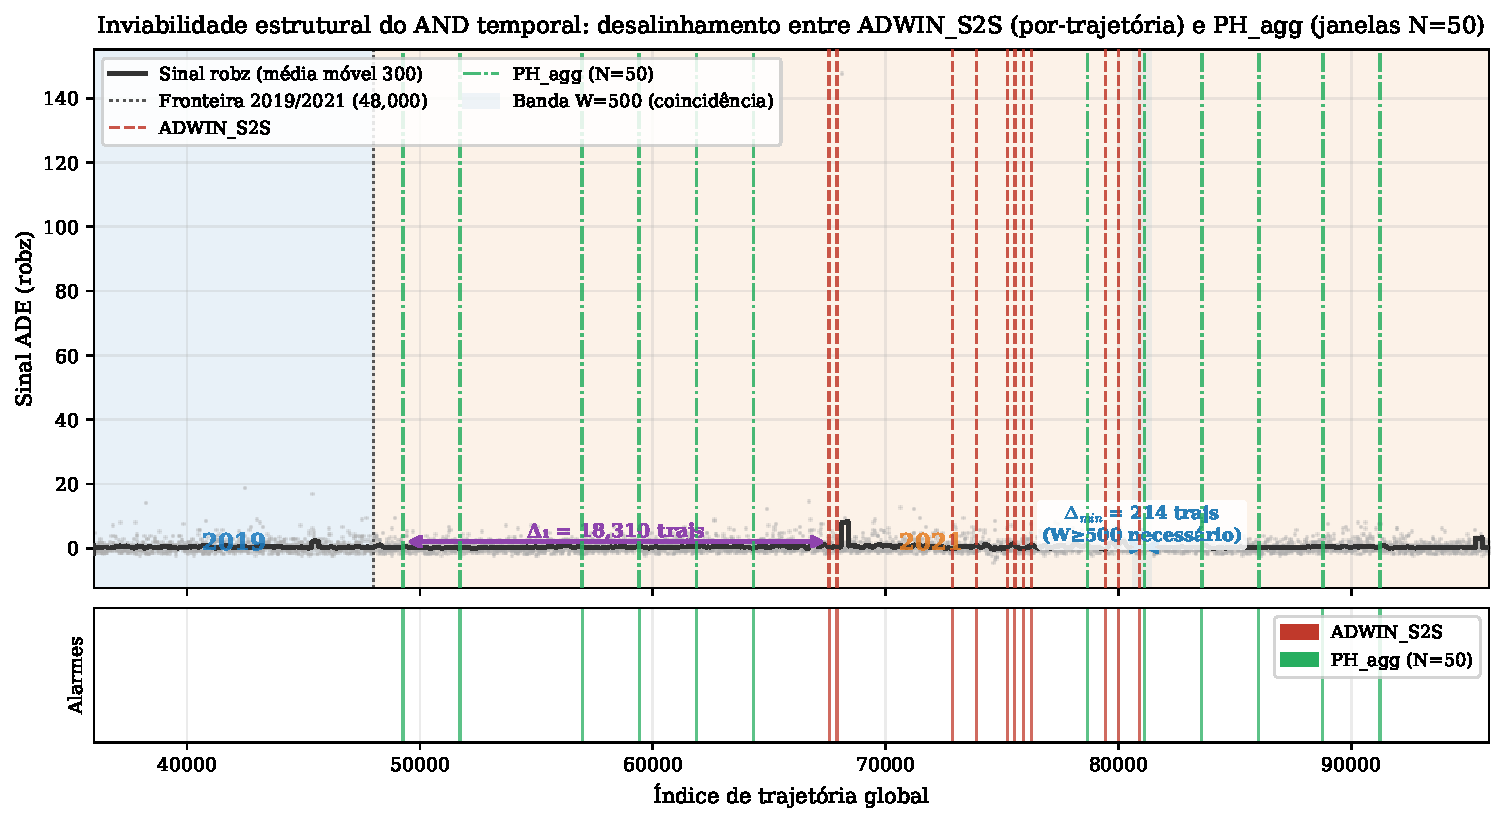
\includegraphics[width=0.95\linewidth]{and_infeasibility}
\caption{\textbf{Inviabilidade estrutural do AND temporal} (Fase 4).
         Painel superior: stream de sinal robz com alarmes ADWIN\_S2S
         (azul) e PH\_agg (vermelho); $\Delta_1\!=\!18\,310$ trajs entre
         os primeiros alarmes em 2021 (ADWIN@67585 vs.\ PH@49275).
         Painel inferior: par mais pr\'oximo em todo o stream ---
         $\Delta_{\min}\!=\!214$ entre ADWIN@80911 e PH@81125, ainda
         \emph{acima} de $W$=200. Independente de calibra\c{c}\~ao, o
         AND \'e estruturalmente vazio nessa janela.
         Fonte: \texttt{phase4\_consolidate.py}.}
\label{fig:m9_and_infeasibility}
\end{figure}

\begin{table}[H]
\centering\small
\begin{tabular}{r r r r r l}
\toprule
\textbf{W} & \textbf{$\sim$meses} & \textbf{n\textsubscript{confirmed}} & \textbf{FAR/1k} & \textbf{year\_cov} & \textbf{nota} \\
\midrule
50     & 0{,}0 & 0 & 0{,}000 & 0 & $\Delta_{\min}\!=\!214\!>\!W$ \\
100    & 0{,}0 & 0 & 0{,}000 & 0 & $\Delta_{\min}\!=\!214\!>\!W$ \\
200    & 0{,}1 & 0 & 0{,}000 & 0 & $\Delta_{\min}\!=\!214\!>\!W$ \\
500    & 0{,}1 & 1 & 0{,}000 & 1 & s\'o 2021 \\
1000   & 0{,}2 & 1 & 0{,}000 & 1 & s\'o 2021 \\
2000   & 0{,}5 & 1 & 0{,}000 & 1 & s\'o 2021 \\
5000   & 1{,}2 & 2 & 0{,}000 & 1 & s\'o 2021 \\
10000  & 2{,}5 & 4 & 0{,}000 & 2 & \textbf{W operacionalmente absurdo} \\
20000  & 5{,}0 & 4 & 0{,}000 & 2 & \textbf{W operacionalmente absurdo} \\
\bottomrule
\end{tabular}
\caption{\textbf{Sweep estendido $W$} (Fase 4). Para year\_coverage=2 (i.e.,
         deteta tamb\'em alguma transi\c{c}\~ao p\'os-2021), \'e
         necess\'ario $W\!\geq\!10\,000$ trajs ($\sim$2{,}5 meses
         operacionais). Esse valor \'e operacionalmente absurdo para
         ``coincid\^encia temporal''. \textbf{Conclus\~ao formal: o
         ensemble AND temporal foi testado, caracterizado e rejeitado.}
         Fonte: \texttt{W\_infeasibility\_sweep.csv}.}
\label{tab:m9_p4_wsweep}
\end{table}

\subsubsection{Intervalos de confian\c{c}a de Wilson para FAR=0}

\begin{table}[H]
\centering\small
\begin{tabular}{l r r r l}
\toprule
\textbf{Detetor} & \textbf{$k$ (2019)} & \textbf{$n$ (2019 trajs)} & \textbf{FAR obs./1k} & \textbf{IC Wilson 95\,\%/1k} \\
\midrule
ADWIN\_S2S          & 2 & 48\,000 & 0{,}042 & $[0{,}011;\,0{,}152]$ \\
PH\_agg standalone  & 0 & 48\,000 & 0{,}000 & $[0{,}000;\,0{,}080]$ \\
AND CONFIRMED (W=200) & 0 & 48\,000 & 0{,}000 & $[0{,}000;\,0{,}080]$ \\
\bottomrule
\end{tabular}
\caption{IC Wilson 95\,\% para FAR\textsubscript{2019}. Para
         $k$\,=\,0 alarmes (PH, AND), o limite superior \'e
         0{,}080/1k --- ainda compat\'ivel com o limiar de
         admissibilidade 0{,}20/1k. ADWIN\_S2S \'e a \'unica config
         com $k\!>\!0$ entre os eleg\'iveis multi-ano.}
\label{tab:m9_p4_wilson}
\end{table}

\subsubsection{Recomenda\c{c}\~ao operacional final}

\begin{table}[H]
\centering\small
\begin{tabular}{l l l}
\toprule
\textbf{Par\^ametro} & \textbf{Detetor prim\'ario (ADWIN\_S2S)} & \textbf{Canal OR (Kalman)} \\
\midrule
Modelo           & Seq2Seq & Kalman \\
Detector         & ADWIN+robz $w$=200 & ADWIN+robz $w$=200 \\
$\delta$         & $10^{-7}$ & $10^{-7}$ \\
\texttt{min\_window}   & 600  & 200 \\
\texttt{cooldown}      & 200  & 1000 \\
\texttt{max\_window}   & 2000 & 5000 \\
FAR\textsubscript{2019}/1k    & \textbf{0{,}042} & 0{,}104 \\
year\_coverage   & 5/5 & 5/5 \\
$n_\text{post}$  & 23 & 45 \\
\bottomrule
\end{tabular}
\caption{\textbf{Recomenda\c{c}\~ao operacional do M\^es 9.}
         O ensemble AND(ADWIN\_S2S, PH\_agg) foi testado, caracterizado
         e rejeitado --- n\~ao aparece como recomenda\c{c}\~ao em
         nenhum output da Fase 4.}
\label{tab:m9_recommendation}
\end{table}

\subsubsection{Artefactos do M\^es 9}

\begin{table}[H]
\centering\small
\begin{tabular}{l l}
\toprule
\textbf{Ficheiro} & \textbf{Conte\'udo} \\
\midrule
\texttt{phase1\_results.csv}        & 22 experimentos $\times$ 2 modelos (ADWIN+PH) \\
\texttt{phase2\_results.csv}        & 174 configs $\times$ 2 modelos (3 frentes) \\
\texttt{phase3\_results.csv}        & ensemble AND/OR + sweep $W$ \\
\texttt{phase4\_master\_table.csv}  & 6 candidatos finais ranqueados \\
\texttt{W\_infeasibility\_sweep.csv} & $W\!\in\!\{50,\ldots,20000\}$ com year\_cov\_confirmed \\
\texttt{images/and\_infeasibility.png} & figura 300 dpi: desalinhamento $\Delta_{\min}\!=\!214$ \\
\texttt{PHASE4\_FINAL.md}           & texto completo para o paper (Q1--Q4, IC Wilson, amea\c{c}as) \\
\texttt{PHASE4\_REPORT.md}          & resumo estruturado da Fase 4 \\
\bottomrule
\end{tabular}
\caption{Artefactos do M\^es 9 (em \texttt{Relas/results/drift/mes9\_phase\{1,2,3,4\}/}).}
\label{tab:m9_artefacts}
\end{table}

% ============================================================================
\section{M\^es 10 --- Fechamento das pend\^encias da revis\~ao}
\label{sec:mes10}
% ============================================================================

A revis\~ao para o artigo final identificou quatro pend\^encias
experimentais: (i)~a \textbf{lat\^encia} de detec\c{c}\~ao do detetor
prim\'ario no stream real (completando a tr\'iade
FAR\,+\,cobertura\,+\,lat\^encia \cite{gama2014,lu2019});
(ii)~a valida\c{c}\~ao da \textbf{hip\'otese de independ\^encia} do
stream de 288\,k trajet\'orias, da qual dependem a FAR e o IC de Wilson;
(iii)~o \textbf{ensemble AND de mesma escala temporal}, teste natural da
explica\c{c}\~ao estrutural da Fase 3; e (iv)~o \textbf{EWC no regime
$\lambda\!\geq\!10^5$}, que a an\'alise de escala do M\^es 7 apontava
como potencialmente \'util. As quatro foram fechadas
(scripts \texttt{drift\_analise/mes10\_\{latency, independence,
same\_scale\_ensemble\}.py} e \texttt{model\_analise/ewc\_finetune.py};
sa\'idas em \texttt{Relas/results/drift/mes10\_pendencias/} e
\texttt{Relas/results/mes7/ewc\_results\_highlambda.csv}).

\subsection{Lat\^encia de detec\c{c}\~ao no stream real}

Para cada ano p\'os-2019, mede-se o atraso entre a fronteira do ano no
stream global e o primeiro alarme do detector dentro do ano.
\emph{Conven\c{c}\~ao}: como o drift \'e gradual (sem changepoint formal
ao n\'ivel per-game), a fronteira do ano \'e usada como proxy do onset~---
a lat\^encia reportada \'e portanto um \textbf{limite superior} da
lat\^encia real. Escala: ${\sim}8\,000$ trajet\'orias/jogo, 48\,000/ano.

\begin{table}[H]
\centering\small
\begin{tabular}{l r r r r r r}
\toprule
\textbf{Detector} & & \textbf{2021} & \textbf{2022} & \textbf{2023} & \textbf{2024} & \textbf{2025} \\
\midrule
\multirow{2}{*}{ADWIN\_S2S (prim\'ario)}
  & trajs  & 19\,585 & 2\,481 & 22\,506 & 8\,401 & 16\,432 \\
  & jogos  & 2{,}45  & 0{,}31 & 2{,}81  & 1{,}05 & 2{,}05  \\
\midrule
\multirow{2}{*}{ADWIN\_Kalman (corroborador)}
  & trajs  & 2\,574 & 7\,502 & 1\,791 & 2\,986 & 34\,515 \\
  & jogos  & 0{,}32 & 0{,}94 & 0{,}22 & 0{,}37 & 4{,}31  \\
\midrule
\multirow{2}{*}{Canal OR (m\'inimo dos dois)}
  & trajs  & 2\,574 & 2\,481 & 1\,791 & 2\,986 & 16\,432 \\
  & jogos  & 0{,}32 & 0{,}31 & 0{,}22 & 0{,}37 & 2{,}05  \\
\bottomrule
\end{tabular}
\caption{Lat\^encia do primeiro alarme por ano (robz\_w200 + ADWIN,
         configs finais da Fase 4). O detetor prim\'ario detecta com
         atraso de 0{,}3--2{,}8 jogos; o canal OR/SUSPECTED reduz a
         lat\^encia de pior caso para $\leq$\,0{,}4 jogo em 4/5 anos.
         Fonte: \texttt{latency\_results.csv}.}
\label{tab:m10_latency}
\end{table}

\begin{figure}[H]
\centering
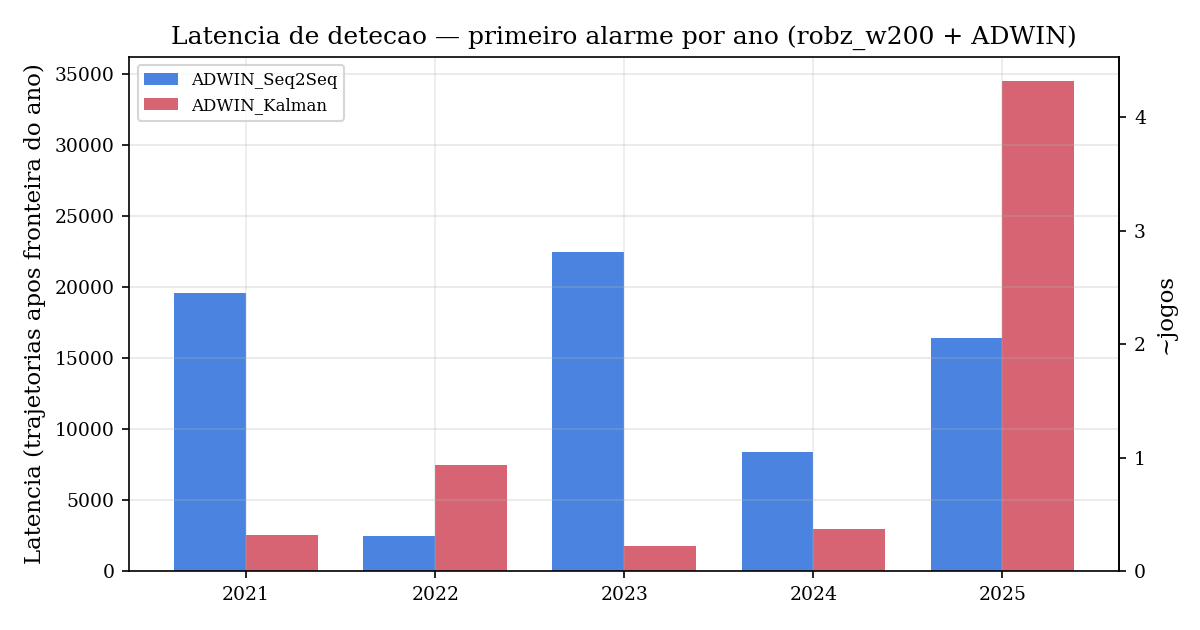
\includegraphics[width=0.8\linewidth]{latency_bars}
\caption{Lat\^encia de detec\c{c}\~ao por ano (barras: trajet\'orias
         ap\'os a fronteira do ano; eixo direito: $\sim$jogos). O Kalman
         corroborador \'e mais r\'apido que o prim\'ario em 4/5 anos~---
         justificativa operacional adicional para o canal OR.}
\label{fig:m10_latency}
\end{figure}

\subsection{Independ\^encia do stream e robustez da FAR}

A FAR por trajet\'oria assume trajet\'orias ${\sim}$i.i.d.\ dentro de
2019~--- hip\'otese que as Limita\c{c}\~oes reconheciam como n\~ao
testada. Tr\^es verifica\c{c}\~oes sobre o bloco 2019
($n\!=\!48\,000$, 6 jogos):

\paragraph{(i) ACF e tamanho amostral efetivo.}
A autocorrela\c{c}\~ao \'e real e substancial: $\rho_1\!=\!0{,}556$ no
ADE bruto e $\rho_1\!=\!0{,}535$ no sinal robz que o detector consome.
O tamanho amostral efetivo
($n_\text{eff} = n/(1+2\sum_k \rho_k)$, soma truncada na banda de
Bartlett) \'e $n_\text{eff}\!\approx\!1\,208$ (2{,}5\,\% de $n$) para o
ADE bruto e $n_\text{eff}\!\approx\!7\,762$ (16{,}2\,\%) para o sinal
robz~--- o pr\'e-processamento robust-z remove a maior parte da
depend\^encia de longo alcance (corte de Bartlett em lag 41 vs.\ lag
500+).

\paragraph{(ii) IC de Wilson conservador.}
Na leitura mais conservadora (manter $k\!=\!2$ alarmes e reduzir a base
para $n_\text{eff}\!=\!7\,762$), o IC de Wilson vai a
$[0{,}071;\,0{,}939]$/1k~--- o limite superior ultrapassa o teto de
admissibilidade de 0{,}20/1k. A taxa pontual observada permanece
0{,}042/1k; o que a corre\c{c}\~ao mostra \'e que, com 6 jogos, a
incerteza honesta sobre a FAR \'e maior do que o IC ing\^enuo sugere.

\paragraph{(iii) Teste por permuta\c{c}\~ao ($B\!=\!200$).}
O pipeline completo (robz + ADWIN final) foi re-executado sobre o bloco
2019 permutado em tr\^es esquemas:

\begin{table}[H]
\centering\small
\begin{tabular}{l l r r r}
\toprule
\textbf{Esquema} & \textbf{estrutura destru\'ida} & \textbf{$k$ m\'edio} & \textbf{[p5; p95]} & \textbf{$P(k \geq 2)$} \\
\midrule
\texttt{blocks} & ordem dos 6 jogos            & 1{,}84 & [1; 2] & 0{,}84 \\
\texttt{within} & autocorr.\ intra-jogo        & 0{,}00 & [0; 0] & 0{,}00 \\
\texttt{full}   & toda a estrutura temporal    & 0{,}00 & [0; 0] & 0{,}00 \\
\bottomrule
\end{tabular}
\caption{Alarmes 2019 do pipeline final sob permuta\c{c}\~ao
         (observado: $k\!=\!2$). Permutar a \emph{ordem dos jogos}
         n\~ao altera a FAR ($k$ m\'edio 1{,}84); destruir a
         autocorrela\c{c}\~ao \emph{intra-jogo} zera os falsos alarmes.
         Fonte: \texttt{permutation\_far.csv}.}
\label{tab:m10_perm}
\end{table}

\textbf{Leitura.} Os dois falsos alarmes de 2019 v\^em precisamente da
estrutura local autocorrelacionada (rajadas dentro de jogo): um stream
2019 i.i.d.-izado produz \emph{zero} alarmes. A viola\c{c}\~ao da
hip\'otese de independ\^encia \'e portanto \textbf{conservadora na
dire\c{c}\~ao certa}~--- ela infla a FAR estimada em rela\c{c}\~ao ao
null i.i.d., de modo que a admissibilidade do detetor n\~ao \'e artefato
da depend\^encia serial. O custo honesto \'e o IC mais largo do item
(ii), consequ\^encia do tamanho amostral (6 jogos), n\~ao do detector.

\begin{figure}[H]
\centering
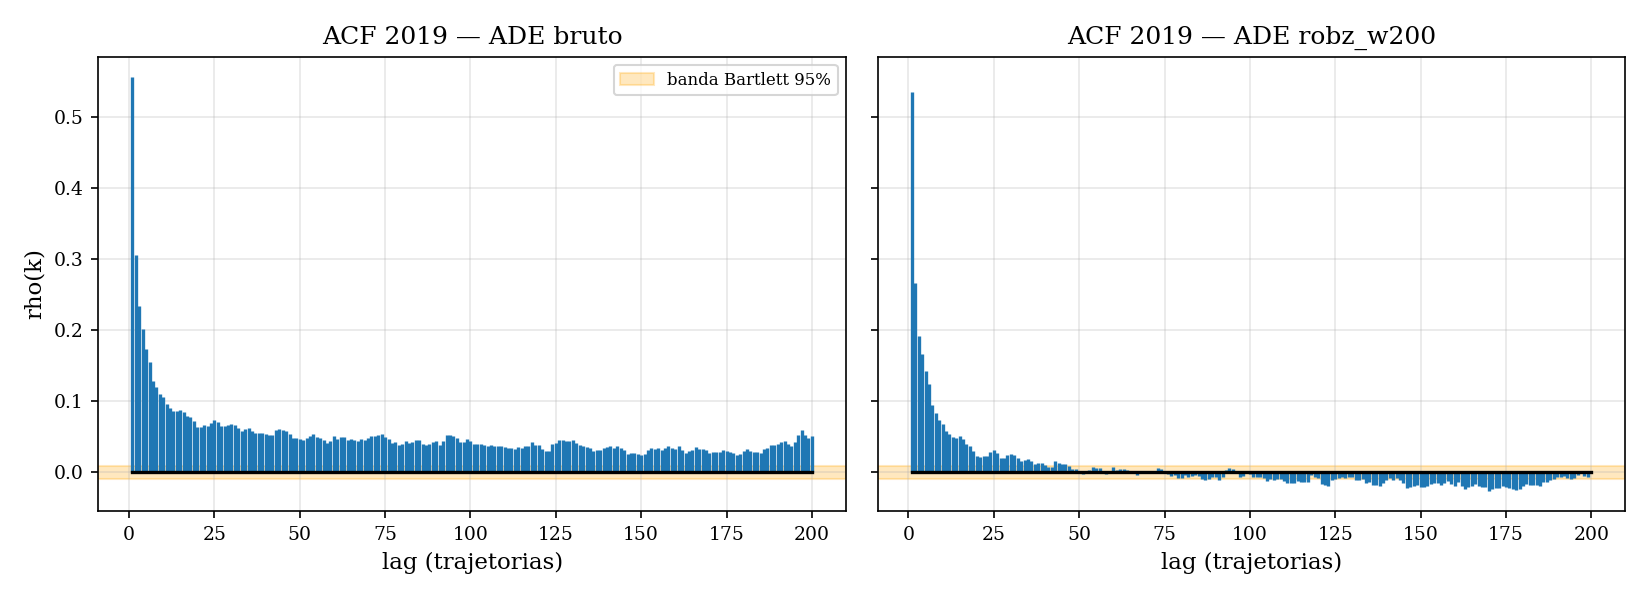
\includegraphics[width=0.95\linewidth]{acf_2019}
\caption{ACF do bloco 2019 (esq.: ADE bruto; dir.: sinal robz\_w200)
         com banda de Bartlett 95\,\%. O robust-z encurta drasticamente
         a mem\'oria do sinal (corte em lag 41 vs.\ 500+).}
\label{fig:m10_acf}
\end{figure}

\subsection{Ensemble AND de mesma escala temporal}

A Fase 3 atribuiu a inviabilidade do AND ao desalinhamento de escalas
(ADWIN por trajet\'oria vs.\ PH por janela de 50). O teste natural dessa
explica\c{c}\~ao \'e alinhar as escalas: dois ADWIN por trajet\'oria,
um sobre o ADE e outro sobre \texttt{accel\_p95} da janela de entrada
da pr\'opria trajet\'oria (extra\'ida sem infer\^encia do modelo, a
partir de $v_x, v_y$ desnormalizados; 3{,}7\,M janelas processadas),
ambos com robz\_w200.

\begin{table}[H]
\centering\small
\begin{tabular}{l r r r r l}
\toprule
\textbf{Config} & \textbf{W} & \textbf{n\textsubscript{conf}} & \textbf{FAR/1k} & \textbf{year\_cov} & \textbf{anos} \\
\midrule
AND(ADE, ACC) & 50   & 4  & 0{,}021 & 3/5 & 2021, 2023, 2024 \\
AND(ADE, ACC) & 200  & 7  & 0{,}021 & 3/5 & 2021, 2023, 2024 \\
AND(ADE, ACC) & 2000 & 10 & 0{,}021 & 4/5 & +2022 \\
\midrule
ADWIN\_ADE standalone & --- & 25  & 0{,}042 & 5/5 & todos \\
ADWIN\_ACC standalone & --- & 114 & 0{,}271 & 5/5 & todos (\emph{inadmiss\'ivel}) \\
\bottomrule
\end{tabular}
\caption{Ensemble de mesma escala (M\^es 10).
         $\Delta_{\min}(\text{ADE},\text{ACC})\!=\!3$ trajet\'orias
         (vs.\ 214 na Fase 3): com escalas alinhadas h\'a coincid\^encia
         j\'a em $W\!=\!50$. Fonte: \texttt{same\_scale\_ensemble.csv}.}
\label{tab:m10_samescale}
\end{table}

\textbf{Leitura.} O resultado confirma o diagn\'ostico da Fase 3 e o
refina em tr\^es pontos:
(i)~\emph{o desalinhamento era mesmo a causa}: $\Delta_{\min}$ cai de
214 para 3 trajet\'orias quando as escalas s\~ao alinhadas, e o AND
deixa de ser estruturalmente vazio;
(ii)~\emph{o AND repara um detector individualmente inadmiss\'ivel}: o
ADWIN sobre acelera\c{c}\~ao tem FAR\,=\,0{,}271/1k (consistente com o
achado do KSWIN: features cinem\'aticas variam naturalmente dentro de
2019), mas o gate AND reduz a FAR do conjunto para 0{,}021/1k~---
metade da FAR do prim\'ario;
(iii)~\emph{o custo \'e cobertura}: os anos de drift fraco (2022, 2025)
n\~ao geram coincid\^encias com $W\!\leq\!1000$, de modo que, pela regra
de decis\~ao (cobertura primeiro), \textbf{o ADWIN\_S2S standalone
segue sendo a recomenda\c{c}\~ao}~--- agora com a alternativa AND de
mesma escala caracterizada como op\c{c}\~ao de alta especificidade
para cen\'arios em que falsos alarmes s\~ao mais custosos que
lat\^encia de cobertura.

\begin{figure}[H]
\centering
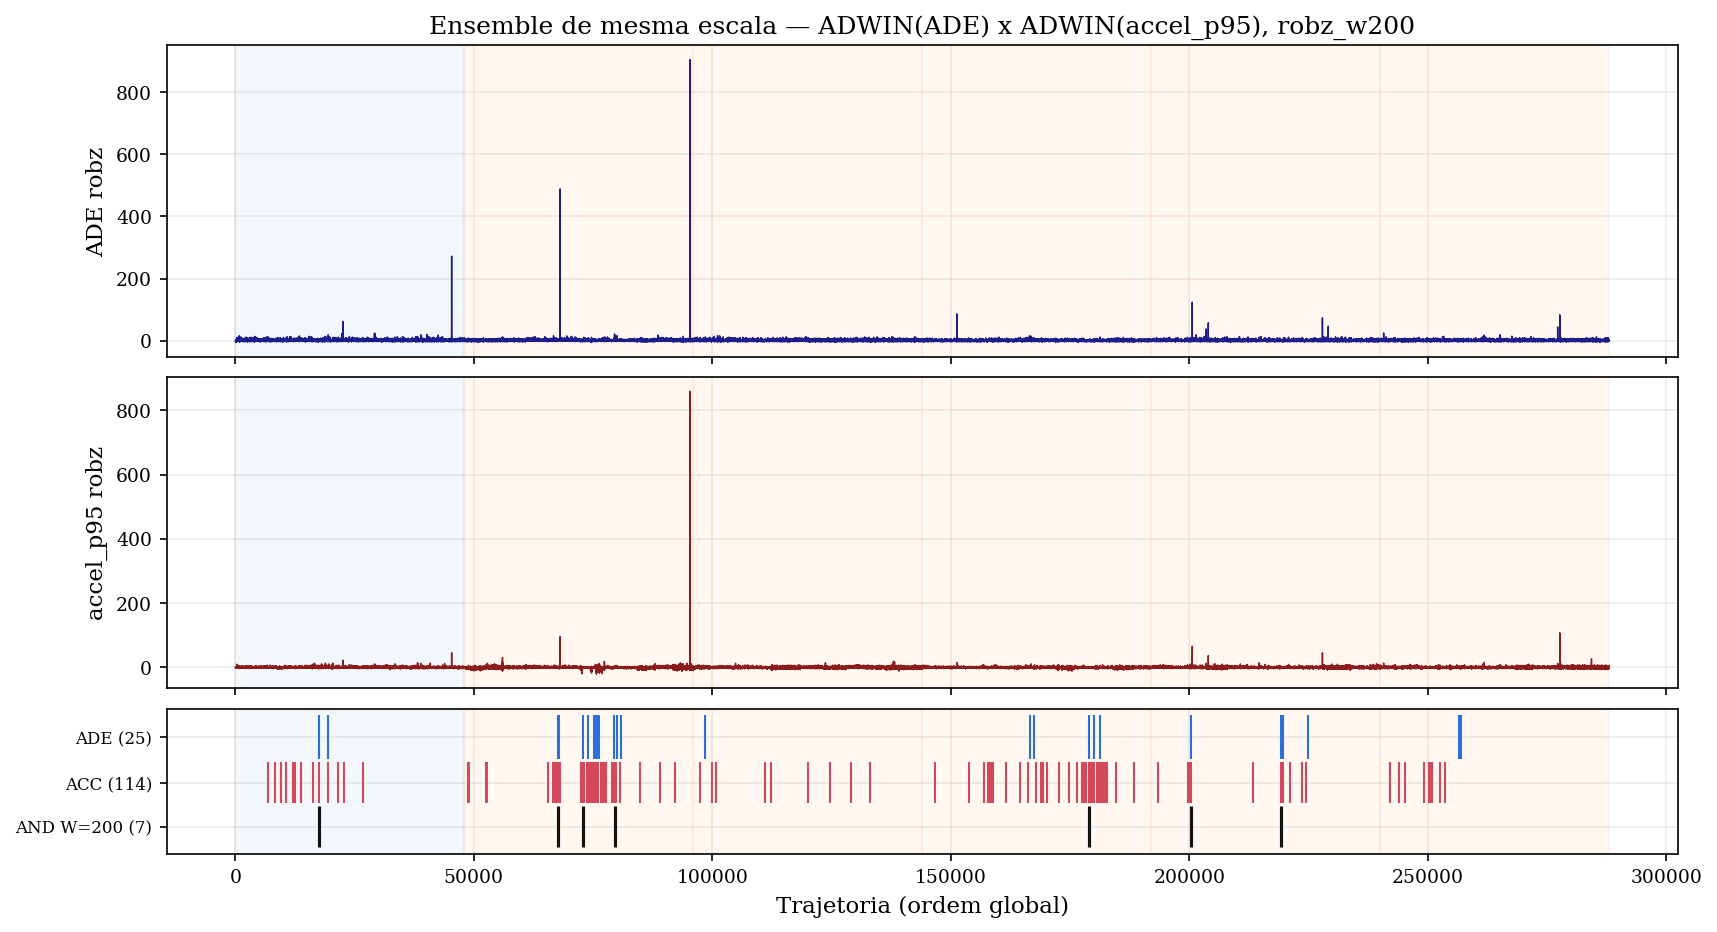
\includegraphics[width=0.95\linewidth]{ensemble_stream}
\caption{Ensemble de mesma escala: sinais robz de ADE (topo) e
         \texttt{accel\_p95} (meio) com rasters de alarmes e canal
         AND $W$=200 (baixo).}
\label{fig:m10_samescale}
\end{figure}

\subsection{EWC no regime $\lambda\!\geq\!10^5$}

O sweep complementar $\lambda\!\in\!\{10^5, 10^6, 10^7\}$ (mesmo
protocolo do M\^es 7: 5 \'epocas, \texttt{lr}=$10^{-5}$,
\texttt{n\_unfreeze}=2) fecha a \'ultima lacuna do resultado do EWC:
\texttt{cat\_ratio}\,$\in [0{,}449;\,0{,}452]$ e
\texttt{recovery}\,$\in [-12{,}8;\,-11{,}8]\,\%$, indistingu\'iveis de
$\lambda\!=\!0$ (0{,}444). A Tabela~\ref{tab:ewc} consolida as sete
configura\c{c}\~oes. O resultado negativo da regulariza\c{c}\~ao de
Fisher \'e definitivo ao longo de 8 ordens de grandeza de $\lambda$;
ver discuss\~ao na Se\c{c}\~ao~\ref{sec:ewc}.

% ============================================================================
\section{An\'alise cr\'itica e tese central (revisada ap\'os M\^es 9)}
% ============================================================================

\subsection{\'Arvore de decis\~ao para o cen\'ario do trabalho}

No in\'icio do quarto m\^es de pesquisa, foram definidos tr\^es \textbf{cen\'arios poss\'iveis}~--- perfis de resultado que o estudo poderia encontrar~--- para guiar a dire\c{c}\~ao das an\'alises seguintes. A id\'eia de uma ``\'arvore de decis\~ao'' \'e simples: come\c{c}a-se pela pergunta mais b\'asica (``o drift \'e real ou \'e confundimento?''), e dependendo da resposta, avalia-se a pr\'oxima (``o modelo degrada muito ou pouco?''). Cada ramo leva a um cen\'ario com hip\'oteses e conclus\~oes diferentes.

\begin{itemize}[leftmargin=1.4em,itemsep=6pt]
    \item \textbf{Cen\'ario 1}: o drift aparente seria um \emph{confundimento}
          entre divis\~oes~--- isto \'e, a piora do modelo seria causada n\~ao
          por mudan\c{c}a real no estilo de jogo, mas pelo fato de o dataset
          de 2019 misturar jogos de Divis\~ao A e B enquanto os datasets de
          2022--2025 s\~ao todos Divis\~ao A. \textbf{N\~ao se aplica}: os
          dados dispon\'iveis n\~ao incluem Divis\~ao B, de modo que n\~ao \'e
          poss\'ivel testar essa hip\'otese; al\'em disso, $\Delta_A \approx
          0{,}40$\,mm \'e positivo e persistente, indicando drift real.
    \item \textbf{Cen\'ario 2}: o drift seria severo o suficiente para que
          adapta\c{c}\~ao simples (fine-tuning com poucos exemplos) n\~ao fosse
          suficiente, exigindo retreino completo ou arquitetura nova.
          \textbf{N\~ao se aplica}: o excesso de ADE \'e pequeno (0{,}4\,mm
          em uma escala de dezenas de mm) e a recupera\c{c}\~ao mediana por
          importance weighting \'e $\approx 63\,\%$~--- o modelo degrada, mas
          moderadamente, e a adapta\c{c}\~ao parcial \'e vi\'avel.
    \item \textbf{Cen\'ario 3} (descritivo + detec\c{c}\~ao operacional):
          o drift \'e real e mensur\'avel, a adapta\c{c}\~ao \'e
          \emph{parcialmente} eficaz, e o trabalho concentra-se em
          \textbf{caracterizar} o drift (quais features mudam, em que per\'iodo,
          com que magnitude) e em desenvolver um \textbf{detetor online
          operacional} que avise o engenheiro quando retreinar.
          \textbf{Escolhido}.
\end{itemize}

\subsection{Tese central --- Cen\'ario~3 reformulado}

A \textbf{tese central} \'e a afirma\c{c}\~ao principal que este trabalho defende, suportada por evid\^encias num\'ericas convergentes. Em resumo:

O drift no Seq2Seq para trajet\'orias SSL \'e \textbf{real},
\textbf{intra-divis\~ao} (ocorre dentro da Divis\~ao A, ou seja, n\~ao \'e
um artefato de misturar divis\~oes) e \textbf{direcionalmente covariate}
(o tipo de drift em que as caracter\'isticas de entrada do modelo mudam,
n\~ao a rela\c{c}\~ao entre entrada e sa\'ida): o classifier two-sample
test rejeita a hip\'otese de igualdade distribucional em todos os anos
($p\!<\!10^{-3}$), e a fra\c{c}\~ao do excesso de ADE atribu\'ivel a esse
covariate shift est\'a entre 9 e 72\,\% (LSIF 59--72\,\%, RuLSIF 9--23\,\%,
classifier cov.\ 22--51\,\%~--- Tabela~\ref{tab:iw_decomp}), com
\texttt{accel\_p99} como a feature dominante segundo o LSIF marginal
(o percentil 99 da acelera\c{c}\~ao~--- representa os movimentos mais
bruscos). Contudo, a adapta\c{c}\~ao por fine-tuning leve
\'e severamente prejudicada por \emph{catastrophic interference}
(o modelo ``esquece'' o que aprendeu antes ao ser retreinado com dados novos).
\textbf{O M\^es 9 acrescenta uma camada operacional}: sobre o stream
de 288\,k trajet\'orias com pr\'e-processamento robust-z, identifica-se
um detetor online vi\'avel (ADWIN\_S2S, FAR\textsubscript{2019}=0{,}042/1k,
year\_coverage=5/5).

\paragraph{Reposicionamento ap\'os M\^es~6 e revis\~ao final ap\'os M\^es~9.}
Uma nota sobre \textbf{granularidade} \'e essencial para entender a
evolu\c{c}\~ao das conclus\~oes. \textbf{Granularidade per-game} significa
que cada ponto de dados \'e a m\'edia de ADE de um jogo inteiro: com 6 jogos
por ano e 5 anos de dados (2020--2025), temos apenas 36 pontos no total.
\textbf{Granularidade per-trajet\'oria} significa que cada ponto \'e uma
trajet\'oria individual: com $\approx$57\,600 trajet\'orias por ano, temos
288\,000 pontos. Detectores estat\'isticos precisam de muitos pontos para
funcionar~--- 36 \'e pouco demais.

A leitura inicial dos M\^es 1--5 apoiava a tese central \emph{tamb\'em} em
detec\c{c}\~ao formal de changepoint (ADWIN/PH online + Pelt offline).
O M\^es 6 mostrou que essas detec\c{c}\~oes n\~ao sobrevivem ao escrut\'inio
formal \emph{na granularidade per-game}. O M\^es 9 mostrou que \emph{na
granularidade per-trajet\'oria com pr\'e-processamento adequado} elas
funcionam bem. \textbf{A reposi\c{c}\~ao final \'e:}
\begin{enumerate}[leftmargin=1.4em,itemsep=2pt]
    \item Per-game (36 pontos/ano): detec\c{c}\~ao formal n\~ao funciona;
          a tese descritiva ap\'oia-se em decomposi\c{c}\~ao IW
          (importance weighting~--- estima\c{c}\~ao de quanto cada tipo de
          trajet\'oria est\'a sobre- ou sub-representada em cada ano).
    \item Per-trajet\'oria (288\,k stream): detec\c{c}\~ao funciona bem
          com ADWIN+robz $w$=200 (M\^es 9).
    \item Ensemble AND temporal entre ADWIN e PH \'e estruturalmente
          invi\'avel ($\Delta_{\min}\!=\!214$\,$>$\,$W$=200; cobertura
          $\geq$2/5 s\'o com $W\!\geq\!10\,000$) --- testado,
          caracterizado e rejeitado (os dois detectores disparam com
          atrasos de milhares de trajet\'orias entre si, o que torna o
          AND de coincid\^encia inoperante para janelas razo\'aveis).
\end{enumerate}

\subsubsection{Suporte num\'erico amalgamado}

\begin{enumerate}[leftmargin=1.6em,itemsep=2pt]
    \item $\Delta_A \approx 0{,}40$\,mm positivo e persistente em
          2022--2025 (Tabela~\ref{tab:division}).
    \item Recovery LSIF mediana $\approx 65\,\%$ (range 59--72\,\%);
          RuLSIF mediana $\approx 12\,\%$ (range 9--23\,\%);
          classifier cov.\ mediana $\approx 31\,\%$ (range 22--51\,\%) ---
          os tr\^es estimadores concordam em sinal mas variam em
          magnitude (Tabela~\ref{tab:iw_decomp}). Todos os anos
          significativos a $p\!<\!10^{-3}$ pelo classifier two-sample test.
    \item \texttt{accel\_p99} lidera ranking de features
          (Tabela~\ref{tab:iw_feat}).
    \item Fine-tuning ing\^enuo: \texttt{cat\_ratio}=0{,}82 (M\^es 3,
          Tabela~\ref{tab:retrain}); reduzido a 0{,}44 com EWC
          (M\^es 7, Tabela~\ref{tab:ewc}).
    \item Pelt mBIC monot\^onico: $K^*\!=\!0$ ao n\'ivel de 36 jogos
          (Figura~\ref{fig:m2_bic}).
    \item \textbf{Detec\c{c}\~ao operacional viavel} sobre stream
          per-trajetoria com robz $w$=200: FAR=0{,}042/1k,
          year\_coverage=5/5 (Tabela~\ref{tab:m9_master}, M\^es 9).
    \item \textbf{Ensemble AND invi\'avel}: $\Delta_{\min}\!=\!214$;
          year\_coverage=2 exige $W\!\geq\!10\,000$ ($\sim$2{,}5 meses)
          --- absurdo (Tabela~\ref{tab:m9_p4_wsweep}, M\^es 9).
\end{enumerate}

\subsection{Leitura cruzada das figuras}

\begin{itemize}[leftmargin=1.4em,itemsep=2pt]
    \item \textbf{O drift afeta a cauda mais do que a m\'edia}:
          Figura~\ref{fig:m1_p99}, Figura~\ref{fig:m1_hist} e
          Tabela~\ref{tab:tail} concordam.
    \item \textbf{Acelera\c{c}\~ao \'e a feature dominante}:
          Figura~\ref{fig:m1_ade_vs} (regress\~ao), Figura~\ref{fig:m1_corr}
          (Spearman), Figura~\ref{fig:m1_window_accel} (KS por janela), e
          Tabela~\ref{tab:iw_feat} (LSIF marginal). \emph{Quatro
          evid\^encias independentes alinhadas}.
    \item \textbf{Concept drift residual existe}: recovery LSIF $\leq\,72\,\%$
          (Figura~\ref{fig:m3_iw_b}; teto RuLSIF mais baixo, 23\,\%,
          Tabela~\ref{tab:iw_decomp}) + fine-tuning falha em recuperar o
          restante (Tabela~\ref{tab:retrain}).
    \item \textbf{Detec\c{c}\~ao online funciona no stream completo}:
          Figura~\ref{fig:m9_grid_streams_a} (top-5 streams ADWIN+robz),
          Figura~\ref{fig:m9_ensemble_stream} (3 canais),
          Tabela~\ref{tab:m9_master} (master table). \emph{Tr\^es
          ang\^ulos confirmam o detetor prim\'ario}.
    \item \textbf{AND temporal \'e invi\'avel}:
          Figura~\ref{fig:m9_and_infeasibility} (desalinhamento) +
          Figura~\ref{fig:m9_coincidence_sweep} (sweep) +
          Tabela~\ref{tab:m9_p4_wsweep} (W=10\,000 $\sim$2{,}5 meses).
\end{itemize}

% ============================================================================
\section{Limita\c{c}\~oes honestas}
% ============================================================================

\begin{itemize}[leftmargin=1.4em,itemsep=4pt]
    \item \textbf{Divis\~ao\,B ausente.} O RoboCup SSL tem duas divis\~oes de competi\c{c}\~ao: Divis\~ao A (times mais avan\c{c}ados) e Divis\~ao B (times em desenvolvimento). Nenhum dos conjuntos de dados dispon\'iveis corresponde \`a Divis\~ao B; todos os dados de 2022--2025 s\~ao Divis\~ao A. Isso impede testar se o drift observado seria diferente entre divis\~oes~--- uma quest\~ao que permanece em aberto.

    \item \textbf{Detectores online sem poder estat\'istico ao n\'ivel per-game.} A calibra\c{c}\~ao por ARL (M\^es 6) confirmou que ADWIN e PH n\~ao conseguem rejeitar H\textsubscript{0} (a hip\'otese nula de ``sem drift'') no stream por jogo ($n{=}36$ pontos, um por jogo). O problema \'e que 36 pontos s\~ao poucos para qualquer teste estat\'istico detectar drift gradual. O M\^es 9 contorna isso operando \emph{por trajet\'oria} (288\,k pontos), o que depende da hip\'otese de independ\^encia entre trajet\'orias consecutivas. \textbf{O M\^es 10 testou essa hip\'otese} (Se\c{c}\~ao~\ref{sec:mes10}): a autocorrela\c{c}\~ao \'e real ($\rho_1\!\approx\!0{,}54$; $n_\text{eff}\!\approx\!7\,762$ no sinal robz, 16\,\% de $n$), e o IC de Wilson conservador da FAR alarga para $[0{,}071;\,0{,}939]$/1k. Por\'em o teste por permuta\c{c}\~ao mostra que a depend\^encia serial \emph{infla} a FAR (streams 2019 i.i.d.-izados produzem zero alarmes): a viola\c{c}\~ao \'e conservadora na dire\c{c}\~ao certa e a admissibilidade do detetor n\~ao \'e artefato dela. O que permanece como limita\c{c}\~ao \'e a largura honesta do IC, consequ\^encia dos 6 jogos de 2019.

    \item \textbf{ADE single-mode, n\~ao min-ADE\textsubscript{$K$}.} O Seq2Seq neste trabalho produz \emph{uma \'unica} previs\~ao determin\'istica por trajet\'oria (single-mode). Modelos estoc\'asticos modernos como Trajectron++ \cite{salzmann2020} e AgentFormer \cite{yuan2021} geram $K$ trajet\'orias hipot\'eticas diferentes e s\~ao avaliados pelo \textbf{min-ADE\textsubscript{$K$}}~--- a dist\^ancia m\'inima entre as $K$ previs\~oes e a trajet\'oria real. Essa m\'etrica \'e mais justa para modelos multimodo. Resultados com min-ADE\textsubscript{$K$} n\~ao s\~ao diretamente compar\'aveis aos com ADE single-mode.

    \item \textbf{EWC reduz \texttt{cat\_ratio} via \texttt{lr}, n\~ao via Fisher.} O ganho real em rela\c{c}\~ao ao M\^es~3 adv\'em da taxa de aprendizado muito baixa ($lr\!=\!10^{-5}$) e do congelamento do encoder~--- n\~ao da regulariza\c{c}\~ao EWC propriamente dita. A diagonal de Fisher \'e n\~ao nula (\texttt{mean diag}$\approx 6{,}7\!\times\!10^{-7}$), mas o sweep completo $\lambda\!\in\!\{0, 50, 500, 5000, 10^5, 10^6, 10^7\}$ (M\^eses 7 e 10) mostra \texttt{cat\_ratio} est\'avel em $0{,}44$--$0{,}45$ em todo o intervalo: a regulariza\c{c}\~ao de Fisher n\~ao adiciona sinal em nenhum regime testado. O resultado negativo \'e definitivo para esta arquitetura/convers\~ao; a alternativa por explorar \'e replay ou retreino do encoder.

    \item \textbf{Tamanho amostral pequeno.} Apenas 6 jogos por ano~--- com este volume, os ICs s\~ao amplos, especialmente para anos com baixo excesso (2022, excesso\,=\,0{,}23\,mm). O IID bootstrap original reamostrava trajet\'orias individualmente, ignorando a correla\c{c}\~ao intra-jogo; o \textbf{block bootstrap} (bloco\,=\,jogo, implementado em itera\c{c}\~ao p\'os-M\^es\,9) revelapag ICs honestamente mais largos e compat\'iveis com o tamanho real da amostra. Para 2022, cujo excesso \'e pr\'oximo de zero, o block bootstrap \'e inst\'avel (denominador da recovery tende a zero); o IC IID \'e reportado para esse ano. Mais jogos por ano reduziriam a incerteza significativamente.

    \item \textbf{Concept drift residual n\~ao \'e isolado por feature.} A fra\c{c}\~ao do excesso de ADE n\~ao explicada por covariate shift nas features cinem\'aticas medidas (velocidade, acelera\c{c}\~ao, curva) depende do estimador: $\approx 28$--41\,\% sob LSIF, $\approx 77$--91\,\% sob RuLSIF; o intervalo plaus\'ivel para a componente residual \'e [28; 91]\,\%. N\~ao sabemos se esse residu\'o \'e: (a) covariate shift em features n\~ao medidas; (b) concept drift real (mudan\c{c}a nas estrat\'egias de jogo); ou (c) simplesmente ru\'ido amostral. A discord\^ancia LSIF/RuLSIF refor\c{c}a a hip\'otese de que parte do que LSIF atribu\'ia a covariate shift est\'a, na verdade, na cauda extrema de \texttt{accel\_p99} onde os pesos LSIF s\~ao numericamente inst\'aveis.

    \item \textbf{Monocultura de evid\^encia no covariate shift.} O n\'umero ``59--72\,\%'' tinha uma \'unica fonte metodol\'ogica (LSIF). Em itera\c{c}\~ao p\'os-M\^es\,9, foram implementados dois validadores independentes: (i)~\textbf{RuLSIF} \cite{yamada2013}, estimador robusto com pesos limitados por $1/\alpha$, que reduz a vari\^ancia sob cauda pesada e \'e comparado ao LSIF; (ii)~teste de duas amostras via \textbf{classificador} \cite{lopezpaz2017}, que detecta covariate shift sem assumir forma para a raz\~ao de densidades. Os resultados s\~ao discutidos na Tabela~\ref{tab:iw_decomp}.

    \item \textbf{Ensemble AND invi\'avel entre escalas distintas (M\^es 9); vi\'avel mas subordinado na mesma escala (M\^es 10).} A inviabilidade da Fase 3 \'e estrutural \`a configura\c{c}\~ao ADWIN-por-trajetoria + PH-por-janela. O teste de mesma escala do M\^es 10 (dois ADWIN por trajet\'oria: ADE + \texttt{accel\_p95}) confirma o diagn\'ostico: $\Delta_{\min}$ cai de 214 para 3 trajet\'orias e o AND passa a produzir alarmes confirmados j\'a com $W\!=\!50$. Por\'em o AND de mesma escala reduz a cobertura (3/5 anos com $W\!\leq\!1000$) porque o detector de acelera\c{c}\~ao \'e individualmente inadmiss\'ivel (FAR\,=\,0{,}271/1k) e os anos de drift fraco (2022, 2025) n\~ao geram coincid\^encias~--- o ADWIN\_S2S standalone segue sendo a recomenda\c{c}\~ao pela regra de decis\~ao (cobertura primeiro).

    \item \textbf{Pr\'e-processamento robust-z assume estacionariedade local.} O robust-z com janela $w$=200 funciona porque o drift \'e \emph{gradual}: a distribui\c{c}\~ao muda lentamente ao longo de meses. Isso significa que dentro de uma janela de 200 trajet\'orias ($\approx$ algumas horas de jogo), a distribui\c{c}\~ao \'e aproximadamente est\'avel~--- o que justifica normalizar por ela. Sob drift \emph{abrupto} (mudan\c{c}a instant\^anea), a janela de 200 trajet\'orias faria a normaliza\c{c}\~ao absorver o pr\'oprio sinal de drift, tornando-o indetect\'avel~--- o robusto-z ``engolaria'' exatamente o que tenta detectar.
\end{itemize}

% ============================================================================
\section{Pr\'oximos passos}
% ============================================================================

\begin{enumerate}[leftmargin=1.6em,itemsep=2pt]
    \item \textit{(Conclu\'ido M\^es 6)} Calibra\c{c}\~ao de ADWIN/PH por
          ARL sint\'etico; curva de lat\^encia corrigida; valida\c{c}\~ao
          do Pelt por BOCPD + gamma.
    \item \textit{(Conclu\'ido M\^es 7)} EWC \cite{kirkpatrick2017} com
          sweep $\lambda$\,$\in\!\{0, 50, 500\}$: \texttt{cat\_ratio}
          0{,}82\,$\to$\,0{,}44.
    \item \textit{(Conclu\'ido M\^es 8)} Reescrita das se\c{c}\~oes
          introdut\'orias e \emph{related work} integrando $\sim$35
          refer\^encias.
    \item \textit{(Conclu\'ido M\^es 9)} Otimiza\c{c}\~ao em 4 fases:
          (i) pr\'e-processamento \texttt{robz\_w200},
          (ii) grid 174 configs $\times$ 2 modelos $\times$ 3 frentes,
          (iii) ensemble AND/OR + sweep $W$,
          (iv) m\'etrica SNR\textsubscript{smooth}, master table,
          inviabilidade do AND.
          Detetor prim\'ario: ADWIN+robz com
          FAR\textsubscript{2019}=0{,}042/1k, year\_coverage=5/5.
    \item \textit{(Conclu\'ido p\'os-M\^es 9)} \textbf{RuLSIF}~\cite{yamada2013}
          implementado e comparado ao LSIF cl\'assico; block bootstrap (bloco\,=\,jogo)
          substitu\'i o IID bootstrap para ICs honestos; teste de duas amostras
          via classificador \cite{lopezpaz2017} implementado como valida\c{c}\~ao
          independente. Resultados na Tabela~\ref{tab:iw_decomp}.
    \item \textit{(Conclu\'ido M\^es 10)} Fechamento das quatro
          pend\^encias da revis\~ao do artigo (Se\c{c}\~ao~\ref{sec:mes10}):
          latência de detec\c{c}\~ao por ano no stream real;
          valida\c{c}\~ao da hip\'otese de independ\^encia do stream
          (ACF, $n_\text{eff}$, permuta\c{c}\~oes em bloco);
          ensemble AND de mesma escala temporal
          ($\Delta_{\min}$: 214\,$\to$\,3); EWC com
          $\lambda\!\in\!\{10^5,10^6,10^7\}$ (negativo definitivo).
    \item \textit{(Pendente)} Implementa\c{c}\~ao do detetor prim\'ario
          como servi\c{c}o online: integrar ADWIN+robz em um pipeline
          que dispare retreino com cooldown=200.
    \item \textit{(Pendente)} Baseline de adapta\c{c}\~ao por
          \emph{replay} (minibatches 2019+2021) como alternativa ao EWC.
    \item \textit{(Mestrado)} Cobrir Divis\~ao\,B (alvo: 2024+, equipes
          competidoras) e \textbf{minADE\textsubscript{$K$}} ao lado
          do ADE single-mode atual, alinhando com \citet{salzmann2020,yuan2021}.
\end{enumerate}

% ============================================================================
\begin{thebibliography}{99}
% ============================================================================

\bibitem[Efron(1979)]{efron1979}
B. Efron.
\textit{Bootstrap methods: another look at the jackknife}.
The Annals of Statistics 7(1), 1979, p.~1--26.
DOI: 10.1214/aos/1176344552.

\bibitem{adwin}
A. Bifet, R. Gavald\`{a}.
\textit{Learning from time-changing data with adaptive windowing}.
SDM, 2007. DOI: 10.1137/1.9781611972771.42.

\bibitem[Page(1954)]{page_hinkley}
E. S. Page.
\textit{Continuous Inspection Schemes}.
Biometrika 41(1--2), 1954, p.~100--115.
DOI: 10.1093/biomet/41.1-2.100.

\bibitem{kswin}
C. Raab, M. Heusinger, F.-M. Schleif.
\textit{Reactive Soft Prototype Computing for Concept Drift Streams}.
Neurocomputing 416, 2020. DOI: 10.1016/j.neucom.2020.01.119.

\bibitem[Mouss et~al.(2004)]{mouss2004}
H. Mouss, D. Mouss, N. Mouss, L. Sefouhi.
\textit{Test of Page-Hinkley, an approach for fault detection in an
agro-alimentary production system}.
Asian Control Conference, 2004.

\bibitem[Gama et~al.(2014)]{gama2014}
J. Gama, I. \v{Z}liobait\.{e}, A. Bifet, M. Pechenizkiy, A. Bouchachia.
\textit{A survey on concept drift adaptation}.
ACM Computing Surveys 46(4), 2014. DOI: 10.1145/2523813.

\bibitem[Lu et~al.(2019)]{lu2019}
J. Lu, A. Liu, F. Dong, F. Gu, J. Gama, G. Zhang.
\textit{Learning under concept drift: a review}.
IEEE TKDE 31(12), 2019. DOI: 10.1109/TKDE.2018.2876857.

\bibitem{ruptures}
C. Truong, L. Oudre, N. Vayatis.
\textit{Selective review of offline change point detection methods}.
Signal Processing 167, 2020. DOI: 10.1016/j.sigpro.2019.107299.

\bibitem{killick2012}
R. Killick, P. Fearnhead, I. A. Eckley.
\textit{Optimal detection of changepoints with a linear computational cost}.
JASA 107(500), 2012. DOI: 10.1080/01621459.2012.737745.

\bibitem{adams2007}
R. P. Adams, D. J. C. MacKay.
\textit{Bayesian Online Changepoint Detection}.
arXiv:0710.3742, 2007.

\bibitem[Aminikhanghahi and Cook(2017)]{aminikhanghahi2017}
S. Aminikhanghahi, D. J. Cook.
\textit{A survey of methods for time series change point detection}.
KAIS 51, 2017, p.~339--367. DOI: 10.1007/s10115-016-0987-z.

\bibitem{kliep}
M. Sugiyama, T. Suzuki, S. Nakajima, H. Kashima, P. von B\"{u}nau, M. Kawanabe.
\textit{Direct importance estimation for covariate shift adaptation}.
Annals of the Institute of Statistical Mathematics 60(4), 2008.
DOI: 10.1007/s10463-008-0197-x.

\bibitem{sugiyama_book}
M. Sugiyama, M. Kawanabe.
\textit{Machine Learning in Non-Stationary Environments}.
MIT Press, 2012.

\bibitem{kanamori2009}
T. Kanamori, S. Hido, M. Sugiyama.
\textit{A least-squares approach to direct importance estimation}.
JMLR 10, 2009, p.~1391--1445.

\bibitem[Yamada et~al.(2013)]{yamada2013}
M. Yamada, T. Suzuki, T. Kanamori, H. Hachiya, M. Sugiyama.
\textit{Relative density-ratio estimation for robust distribution comparison}.
Neural Computation 25(5), 2013. DOI: 10.1162/NECO\_a\_00442.

\bibitem{lopezpaz2017}
D. Lopez-Paz, M. Oquab.
\textit{Revisiting Classifier Two-Sample Tests}.
ICLR, 2017. arXiv:1610.06545.

\bibitem[Kirkpatrick et~al.(2017)]{kirkpatrick2017}
J. Kirkpatrick, R. Pascanu, N. Rabinowitz \emph{et al.}
\textit{Overcoming catastrophic forgetting in neural networks}.
PNAS 114(13), 2017. DOI: 10.1073/pnas.1611835114.

\bibitem{lesort2020}
T. Lesort, V. Lomonaco, A. Stoian, D. Maltoni, D. Filliat, N. D\'iaz-Rodr\'iguez.
\textit{Continual learning for robotics}.
Information Fusion 58, 2020. DOI: 10.1016/j.inffus.2019.12.004.

\bibitem{alahi2016}
A. Alahi, K. Goel, V. Ramanathan, A. Robicquet, L. Fei-Fei, S. Savarese.
\textit{Social LSTM: Human trajectory prediction in crowded spaces}.
CVPR, 2016. DOI: 10.1109/CVPR.2016.110.

\bibitem[Salzmann et~al.(2020)]{salzmann2020}
T. Salzmann, B. Ivanovic, P. Chakravarty, M. Pavone.
\textit{Trajectron++: Dynamically-feasible trajectory forecasting with
heterogeneous data}.
ECCV, 2020. arXiv:2001.03093.

\bibitem[Yuan et~al.(2021)]{yuan2021}
Y. Yuan, X. Weng, Y. Ou, K. Kitani.
\textit{AgentFormer: Agent-aware transformers for socio-temporal
multi-agent forecasting}.
ICCV, 2021. arXiv:2103.14023.

\bibitem[Steuernagel and Maximo(2022)]{steuernagel2022}
L. Steuernagel, M. R. O. A. Maximo.
\textit{Trajectory Prediction for SSL Robots Using Seq2seq Neural Networks}.
In RoboCup 2022: Robot World Cup XXV, LNCS vol.~13561, pp.~27--39.
Springer, 2023. DOI: 10.1007/978-3-031-28469-4\_3.

\bibitem[Gu et~al.(2022)]{gu2022}
T. Gu, G. Chen, J. Li, C. Lin, Y. Rao, J. Zhou, J. Lu.
\textit{Stochastic Trajectory Prediction via Motion Indeterminacy Diffusion}.
CVPR, 2022. arXiv:2203.13777.

\end{thebibliography}

\end{document}
